% Created 2024-06-10 Δευ 19:12
% Intended LaTeX compiler: pdflatex
\documentclass[11pt]{report}
\usepackage[utf8]{inputenc}
\usepackage[T1]{fontenc}
\usepackage{graphicx}
\usepackage{longtable}
\usepackage{wrapfig}
\usepackage{rotating}
\usepackage[normalem]{ulem}
\usepackage{amsmath}
\usepackage{amssymb}
\usepackage{capt-of}
\usepackage{hyperref}
\usepackage{booktabs}
\usepackage{import}
\usepackage[LGR, T1]{fontenc}
\usepackage[greek, english, american]{babel}
\usepackage{alphabeta}
\usepackage{esint}
\usepackage{mathtools}
\usepackage{esdiff}
\usepackage{makeidx}
\usepackage[acronym]{glossaries}
\usepackage{newfloat}
\usepackage{minted}
\usepackage[a4paper, margin=3cm]{geometry}
\usepackage{chemfig}
\usepackage{svg}
\usepackage[automake]{glossaries-extra}
\usepackage{fancyhdr}
\geometry{a4paper,width=150mm,top=25mm,bottom=25mm}
\makeglossaries
\definecolor{Julia_Blue}{RGB}{0, 154, 250}
\definecolor{Julia_Orange}{RGB}{227, 111, 71}
\definecolor{Julia_Green}{RGB}{62, 164, 76}
\hypersetup{linktoc = all, colorlinks = true, citecolor = Julia_Blue, linkcolor = Julia_Orange, urlcolor = Julia_Green}
\newcommand{\HRule}{\rule{\linewidth}{0.5mm}}
\date{}
\title{ΒΙΟΑΠΟΔΟΜΗΣΗ ΥΠΟΛΕΙΜΜΑΤΩΝ ΤΡΟΦΙΜΩΝ ΚΑΙ ΠΑΡΑΓΩΓΗ ΒΙΟΑΕΡΙΟΥ ΜΕΣΩ ΑΝΑΕΡΟΒΙΑΣ ΧΩΝΕΥΣΗΣ ΣΕ ΕΡΓΑΣΤΗΡΙΑΚΗ ΚΑΙ ΠΙΛΟΤΙΚΗ ΚΛΙΜΑΚΑ Προβλήματα στην αναερόβια χώνευση Μεθόδοι Επεξεργασίας Οξεογένεση Οξικογένεση και Μεθανογένεση Πειραματική Διαδικασία Συζήτηση Αποτελεσμάτων Διπλωματικής Συμπεράσματα Μεταβολικά Μονοπάτια σε Julia}
\hypersetup{
 pdfauthor={Βιδιάνος Γιαννίτσης},
 pdftitle={ΒΙΟΑΠΟΔΟΜΗΣΗ ΥΠΟΛΕΙΜΜΑΤΩΝ ΤΡΟΦΙΜΩΝ ΚΑΙ ΠΑΡΑΓΩΓΗ ΒΙΟΑΕΡΙΟΥ ΜΕΣΩ ΑΝΑΕΡΟΒΙΑΣ ΧΩΝΕΥΣΗΣ ΣΕ ΕΡΓΑΣΤΗΡΙΑΚΗ ΚΑΙ ΠΙΛΟΤΙΚΗ ΚΛΙΜΑΚΑ Προβλήματα στην αναερόβια χώνευση Μεθόδοι Επεξεργασίας Οξεογένεση Οξικογένεση και Μεθανογένεση Πειραματική Διαδικασία Συζήτηση Αποτελεσμάτων Διπλωματικής Συμπεράσματα Μεταβολικά Μονοπάτια σε Julia},
 pdfkeywords={},
 pdfsubject={},
 pdfcreator={Emacs 29.3 (Org mode 9.6.15)}, 
 pdflang={English}}
\makeatletter
\newcommand{\citeprocitem}[2]{\hyper@linkstart{cite}{citeproc_bib_item_#1}#2\hyper@linkend}
\makeatother

\usepackage[notquote]{hanging}
\begin{document}

\renewcommand{\abstractname}{Περίληψη}
\renewcommand{\tablename}{Πίνακας}
\renewcommand{\figurename}{Σχήμα }
\renewcommand{\chaptername}{Κεφάλαιο}
\renewcommand{\chapterautorefname}{Κεφάλαιο}
\renewcommand{\sectionautorefname}{Ενότητα}
\renewcommand{\partname}{Μέρος}
\renewcommand{\appendixname}{Παράρτημα}
\renewcommand{\listfigurename}{Περιεχόμενα Σχημάτων: }
\renewcommand{\listtablename}{Περιεχόμενα Πινάκων: }
\renewcommand\listingscaption{Κώδικας}
\pagestyle{fancy}
\fancyhead{}
\fancyhead[L]{ΕΜΠ, Σχολή ΧΜ, Εργαστήριο ΟΧΤ}
\fancyhead[R]{Βιδιάνος Γιαννίτσης}
\fancyfoot{}
\fancyfoot[L]{\chaptername~\thechapter}
\fancyfoot[C]{\thepage}
\newacronym{fw}{ΥΤ}{υπολείμματα τροφών}
\newacronym{fao}{FAO}{Οργανισμός Τροφίμων και Αγρονομίας των Ηνωμένων Πολιτειών}
\newacronym{co2eq}{$CO_2$-eq}{ισοδύναμο διοξειδίου του άνθρακα}
\newacronym{xyta}{ΧΥΤΑ}{Χώρους Υγειονομικής Ταφής Απορριμάτων}
\newacronym{syngas}{syngas}{αέριο σύνθεσης}
\newacronym{pla}{PLA}{πολυγαλακτικό οξύ}
\newacronym{trl}{TRL}{technology readiness level}
\newacronym{vfa}{VFAs}{πτητικά λιπαρά οξέα}
\newacronym{hrt}{HRT}{υδραυλικός χρόνος παραμονής}
\newacronym{olr}{OLR}{ρυθμός οργανικής φόρτισης}
\newacronym{uasb}{UASB}{αντιδραστήρας ανοδικής ροής διαμέσου στρώσης ιλύος}
\newacronym{mix}{μιξ}{σκεύασμα ενζύμων και μικροοργανισμών}
\newacronym{ad}{ΑΧ}{αναερόβια χώνευση}
\newacronym{ts}{TS}{ολικά στερεά}
\newacronym{vs}{VS}{πτητικά στερεά}
\newacronym{cod}{COD}{χημικά απαιτούμενο οξυγόνο}
\newacronym{scod}{sCOD}{διαλυτό COD}
\newacronym{tcod}{tCOD}{ολικό COD}
\newacronym{pi}{PI}{Process Intensification}
\newacronym{ssf}{SSF}{Solid State Fermentation}
\newacronym{orp}{ORP}{οξειδοαναγωγικό δυναμικό}
\newacronym{emp}{EMP}{μονοπάτι Embden-Meyerhof}
\newacronym{lcfa}{LCFA}{long chain fatty acids}
\newacronym{acet-coa}{Acetyl-CoA}{ακέτυλο συνένζυμο Α}
\newacronym{nad}{NAD$^+$}{nicotinamide adenine dinucleotide}
\newacronym{nadh}{NADH}{nicotinamide adenine dinucleotide hydrogen}
\newacronym{fd}{Fd}{ferredoxins}
\newacronym{dg}{ΔG}{μεταβολή ελεύθερης ενέργειας Gibbs}
\newacronym{abe}{ABE}{ζύμωση ακετόνης-βουτανόλης-αιθανόλης}
\newacronym{ed}{ED}{μονοπάτι Entner-Doudoroff}
\newacronym{pp}{PP}{μονοπάτι Pentose Phosphate}
\newacronym{pk}{PK}{μονοπάτι Phosphoketolase}
\newacronym{am}{AM}{ακετοκλαστικοί μεθανογόνοι}
\newacronym{hm}{YM}{υδρογονοτρόφοι μεθανογόνοι}
\newacronym{zvi}{ZVI}{σίδηρος μηδενικού σθένους}
\newacronym{redox}{redox}{οξειδωαναγογικό δυναμικό}
\newacronym{iht}{IHT}{interspecies hydrogen transfer}
\newacronym{diet}{DIET}{direct interspecies electron transfer}
\newacronym{tvfa}{tVFAs}{συνολικά πτητικά λιπαρά οξέα}
\newacronym{bmp}{BMP}{βιοχημικό δυναμικό μεθανίου}
\newacronym{sma}{SMA}{ειδική μεθανογόνος δραστικότητα της λάσπης}
\newacronym{kel}{ΚΕΛ}{κέντρο επεξεργασίας λυμάτων}
\newacronym{ss}{SS}{αιωρούμενα στερεά}
\newacronym{tss}{TSS}{ολικά αιωρούμενα στερεά}
\newacronym{vss}{VSS}{πτητικά αιωρούμενα στερεά}
\newacronym{hplc}{HPLC}{υγρή χρωματογραφία υψηλής απόδοσης}
\newacronym{si}{S/I}{υποστρώματος προς εμβόλιο}
\newacronym{anova}{ANOVA}{ανάλυση διακύμανσης}
\newacronym{mcfa}{MCFA}{λιπαρά οξέα μέτριας ανθρακικής αλυσίδας}
\newacronym{pha}{PHAs}{πολυ-υδρόξυαλκανοϊκοί εστέρες}

\renewcommand{\contentsname}{Κεφάλαια: }
\begin{titlepage}

\begin{center}
  \begin{minipage}{0.2\textwidth}
    \begin{flushleft}
      \includegraphics[width=1\textwidth]{~/Pictures/ntua_logo.png}\\[0.4cm]    
    \end{flushleft}
  \end{minipage}
  \begin{minipage}{0.75\textwidth}
    \textsc{\bfseries \Large ΕΘΝΙΚΟ ΜΕΤΣΟΒΙΟ ΠΟΛΥΤΕΧΝΕΙΟ}\\[0.2cm]
    \textsc{\bfseries \Large ΣΧΟΛΗ ΧΗΜΙΚΩΝ ΜΗΧΑΝΙΚΩΝ}\\[0.2cm]
    \textsc{\large \bfseries ΤΟΜΕΑΣ IV: ΣΥΝΘΕΣΗ ΚΑΙ ΑΝΑΠΤΥΞΗ ΒΙΟΜΗΧΑΝΙΚΩΝ ΔΙΑΔΙΚΑΣΙΩΝ}\\[0.2cm]
    \textsc{\bfseries \large ΕΡΓΑΣΤΗΡΙΟ ΟΡΓΑΝΙΚΗΣ ΧΗΜΙΚΗΣ \\ ΤΕΧΝΟΛΟΓΙΑΣ}\\[0.2cm]
  \end{minipage}
  \\[2.5cm]

  \HRule \\[0.3cm]
  \Huge Βιοαποδόμηση Υπολειμμάτων Τροφίμων και Παραγωγή Βιοαερίου μέσω Αναερόβιας Χώνευσης σε Εργαστηριακή και Πιλοτική Κλίμακα\\[2.5cm]

  \huge Διπλωματική Εργασία \\[0.3cm]
   \begin{minipage}{0.4\textwidth}
    \begin{flushleft}
      \emph{\LARGE Συγγραφέας:}\\
	\emph{\LARGE Αριθμός Μητρώου:} \\
	\emph{\LARGE e-mail:} \\

	\emph{\LARGE Υπεύθυνος Καθηγητής:}
      \end{flushleft}
    \end{minipage}
    \begin{minipage}{0.4\textwidth}
      \begin{flushright} \large
	\LARGE Βιδιάνος Γιαννίτσης\\
	\LARGE ch19113\\
	\LARGE vidianosgiannitsis@gmail.com \\

	\LARGE Ανέστης Βλυσίδης
      \end{flushright}
    \end{minipage}
    \HRule \\[0.3cm]
  \vfill
{\LARGE Αθήνα, 2024}

\end{center}

\end{titlepage}

\begin{abstract}

\large Τα υπολείμματα τροφών (ΥΤ) αποτελούν μία από τις σημαντικότερες κατηγορίες οργανικών αποβλήτων. Η μη ορθή διαχείριση των ΥΤ επιβαρύνει σημαντικά κάθε έναν από τους τρείς πυλώνες της βιωσιμότητας. Το βασικότερο πρόβλημα στην ορθή διαχείριση τους είναι η περιεκτικότητα τους σε βιοπολυμερή. Οπότε, για να αξιοποιηθούν κατάλληλα, απαιτείται ένα στάδιο υδρόλυσης/βιοαποδόμησης. Ιδανικά, αυτό θα γίνει ενζυμικά για να έχει την καλύτερη απόδοση. Όμως, το υψηλό κόστος ενός ενζυμικού σκευάσματος εμποδίζει την εμπορική εφαρμογή μίας τέτοιας διεργασίας. Μία υποσχόμενη και οικονομικά εφαρμόσιμη λύση είναι η χρήση εμπορικών σκευασμάτων ενζύμων και μικροοργανισμών. Ένα τέτοιο σκεύασμα έχει υψηλή ενζυμική ενεργότητα, οπότε μπορεί να υδρολύσει αποτελεσματικά τα υπολείμματα, αλλά έχει πολύ χαμηλή τιμή σε σχέση με καθαρά ένζυμα. Ακόμη, λόγω της παρουσίας μικροοργανισμών, γίνεται μία ταυτόχρονη ζύμωση των ΥΤ. Σκοπός της παρούσας μελέτης είναι η αναλυτική διερεύνηση της δράσης ενος τέτοιου σκευάσματος για παραγωγή μίας υγρής εκροής πλούσιας σε πτητικά λιπαρά οξέα σε εργαστηριακή και πιλοτική κλίμακα. Η εκροή αυτή μπορεί να χρησιμοποιηθεί για διεργασίες όπως η αναερόβια χώνευση. Στα πειράματα εργαστηριακής κλίμακας, τα οποία διεξάχθηκαν σε αντιδραστήρες διαλείποντος έργου, συνολικού όγκου 1 L, έγινε βελτιστοποίηση της διεργασίας ως προς την θερμοκρασία και την ποσότητα του σκευάσματος που προστίθεται. Μέσω αυτών, βρέθηκε πως η υδρόλυση παράγει την μέγιστη ποσότητα οξεογενών προϊόντων σε θερμοκρασία 40 $^o$C και σε ποσότητα 10 mL σκευάσματος/kg ΥΤ. Στα πειράματα πιλοτικής κλίμακας, τα οποία διεξάχθηκαν σε αντιδραστήρα 300 L ημισυνεχούς λειτουργίας, έγιναν δοκιμές για να εξεταστεί η κλιμάκωση της διεργασίας και εξετάστηκε η ποιότητα της υδρόλυσης ανάλογα με την ποσότητα σκευάσματος και την παροχή νερού. Βρέθηκε πως η παροχή μεγαλύτερης ποσότητας νερού δεν επηρεάζει την υδρόλυση, πέραν της αραίωσης, ενώ η ποσότητα σκευάσματος επηρεάζει αρνητικά την παραγωγή διαλυτού οργανικού φορτίου αν αυξηθεί από 5 $\frac{mL}{kg~ ΥΤ}$ σε 10 $\frac{mL}{kg~ ΥΤ}$ καθώς ο λόγος $\frac{sCOD}{tCOD}$ μεταβάλλεται από $46.1 \pm 12.2 \%$ σε $32.7 \pm 10.3 \%$ κατά την αλλαγή αυτή. Έχοντας βελτιστοποιήσει την διεργασία αυτή, έγιναν και δοκιμές αναερόβιας χώνευσης σε αντιδραστήρες διαλείποντος έργου 500 mL, για να μετρηθεί η παραγωγή βιομεθανίου από τα υδρολύματα αυτά, χρησιμοποιώντας αναερόβια λάσπη από 3 διαφορετικές πηγές, για να διαπιστωθεί η επαναληψιμότητα των πειραμάτων. Παρατηρήθηκε πως τα υδρολύματα με 5 και 10 mL σκευάσματος/kg ΥΤ είχαν την καλύτερη απόδοση. Συγκεκριμένα, το 10 $\frac{mL}{kg ~ΥΤ}$ είχε το χαμηλότερο χρόνο καθυστέρησης και τον υψηλότερο ρυθμό παραγωγής μεθανίου, λόγω της καλύτερης οξεογένεσης. Όμως, είχε χαμηλότερη παραγωγή μεθανίου από το υδρόλυμα με 5 mL σκευάσματος/kg ΥΤ, καθώς είχε χειρότερη υδρόλυση. Σε σύγκριση με ανεπεξέργαστα ΥΤ, τα υδρολύματα αυτά είχαν 4-5 φορές περισσότερη παραγωγή μεθανίου. Τα συμπεράσματα αυτά επαληθεύτηκαν για λάσπες διαφορετικών προελεύσεων και χρησιμοποιώντας υδρόλυμα από εργαστηριακή αλλά και πιλοτική κλίμακα. Συμπερασματικά, η υδρόλυση/βιοαποδόμηση ΥΤ μπορεί να γίνει αποτελεσματικά με ένα εμπορικό σκεύασμα ενζύμων και μικροοργανισμών και το παραγώμενο υδρόλυμα είναι ιδιαίτερα κατάλληλο ως υπόστρωμα για αναερόβια χώνευση. \\


Λέξεις Κλειδιά: Υπολείμματα τροφίμων, Υδρόλυση, Βιοαποδόμηση, Αναερόβια χώνευση, Παραγωγή μεθανίου
\end{abstract}

\renewcommand{\abstractname}{Abstract}
\begin{abstract}

\large Food Waste (FW) is one of the most important categories of organic waste. The improper treatment of FW has a very negative impact in all three of the sustainability pillars. The largest problem in properly trating FW is their biopolymer content. For their proper valorization, a hydrolysis/biodegradation step is necessary. Ideally, this is done using enzymes, as this gives the best yield. However, the high cost of enzymic mixtures makes the commercial application of this process very hard. A promising and economic solution for this is the use of commercial mixtures of enzymes and microorganism. Such a mix has high enzymatic activity, thus can effectively hydrolyze the FW, but has a very low price compared to pure enzymes. Furthermore, due to the microorganisms, the FW is fermented as well as hydrolyzed. The goal of this study is an in-depth analysis of the function of such a mix for the production of a liquid effluent, rich in volatile fatty acids, in lab and pilot scale. This effluent can be used in processes such as anaerobic digestion. In the lab scale experiments, which were conducted in batch reactors of total volume 1 L, the process was optimized for temperature and mix amount. From these experiments, it was found that the maximum amount of acidogenic products were produced at a temperature of 40 $^o$ C and with a mix amount of 10 mL/kg FW. In the pilot scale experiments, which were conducted in a semi-continuous reactor with volume 300 L, scale-up tests were done, as well as tests for the hydrolysis quality when varying the mix amount and water flow. It was found that increasing the water flow did not affect the hydrolysis, while the addition of mix beyond 5 mL/kg FW negatively affected the process, since $\frac{sCOD}{tCOD}$ changed from $46.1 \pm 12.2 \%$ to $32.7 \pm 10.3 \%$ when the mix amount was increased to 10 mL/kg FW. Having optimized this process, anaerobic tests were conducted in batch reactors with volume 500 mL, to assess the biomethane production of these hydrolysates, using sludge from 3 different sources, for reproducibility. It was found that the hydrolysates with 5 and 10 mL mix/kg FW had the best production. Specifically, the hydrolysate with 10 mL mix/kg FW had the lowest lag time and fastest production rate, indicating the best acidogenesis, but had less methane production compared to the hydrolysate with 5 mL mix/kg FW. Compared to untreated FW, the hydrolysates had 4-5 times more methane production. These conclusions were validated for different sludge samples and using both and lab and pilot scale hydrolysates. To conclude, the hydrolysis/biodegradation of FW can be effectively done using a commercial mixture of enzymes and microorganisms and the produced hydrolysate is a very good substrate for anaerobic digestion. \\ 


Keywords: Food waste, Hydrolysis, Biodegradation, Anaerobic digestion, Methane production
\end{abstract}

\chapter*{Ευχαριστίες}
\label{sec:org01eff5a}
Η διπλωματική εργασία αυτή δεν θα ήταν δυνατή χωρίς την βοήθεια και καθοδήγηση που δέχτηκα από τον υπεύθυνο καθηγητή μου κ. Ανέστη Βλυσίδη, με τον οποίο είχα εξαιρετική συννενόηση και συνεργασία. Χάρις αυτόν η εργασία παρουσιάστηκε πρόσφατα στο 14ο Πανελλήνιο Συνέδριο Χημικής Μηχανικής, όπου βραβεύτηκε ως η καλύτερη αναρτημένη εργασία της ημέρας και είμαι ιδιαίτερα ευγνώμων που μου δώθηκε αυτή η ευκαιρία. Ιδιαίτερα πολύτιμη ήταν και η βοήθεια που είχα στην διεξαγωγή των πειραμάτων, αλλά και στη συγγραφή της εργασίας από τους μεταδιδακτορικούς ερευνητές του εργαστηρίου Οργανικής Χημικής Τεχνολογίας Δημοσθένη Τσιβά και Δήμητρα Θεοδόση Παλιμέρη. Και οι δύο ήταν εκεί για ότι χρειάστηκα και η στήριξη τους ήταν πολύ σημαντική για την ολοκλήρωση της εργασίας αυτής.

Ακόμη, νιώθω υπόχρεος στην ομάδα του Statista, οι οποίοι μας πρόσφεραν δωρεάν πρόσβαση σε όλη την ιστοσελίδα τους για μερικούς μήνες. Χάρις αυτό, κατάφερα να βρω πολύ αναλυτικά και ανανεωμένα στατιστικά στοιχεία για το αντικείμενο της μελέτης μου, τα οποία έκαναν την εισαγωγή της εργασίας πολύ πιο ευπαρουσίαστη και ενδιαφέρουσα.

Επίσης όμως θα ήθελα να ευχαριστήσω όλο το εργαστήριο Οργανικής Χημικής Τεχνολογίας, από τα μέλη ΕΔΙΠ κ. Δημήτρη Κουλλά και κ. Λάζαρο Καραογλάνογλου, τον μεταδιδακτορικό ερευνητή Κωνσταντίνο Τζάθα, τους υποψήφιους διδάκτορες Παντελή Μάνακα και Ιωάννα Γουδέλη αλλά και τις φοιτήτριες Ιωάννα Κοροπούλη, Αθανασία Δημητρέλου, Στυλιανή Σταύρου και Νεφέλη Καραγιαννοπούλου που έκαναν τις διπλωματικές τους στο εργαστήριο για την ιδιαίτερα ευχάριστη ατμόσφαιρα που είχε το εργαστήριο, κάτι που έκανε την διεξαγωγή των πειραμάτων της εργασίας μου πολύ πιο ευχάριστη. Τέλος, δεν θα μπορούσα να ολοκληρώσω τις ευχαριστίες χωρίς να πω ευχαριστώ στην οικογένεια και στους φίλους μου, οι οποίοι παρότι δεν έπαιξαν άμεσο ρόλο στην εκπόνηση της εργασίας αυτής, με στηρίζουν καθημερινά με άλλους τρόπους.

\part*{Περιεχόμενα}
\label{sec:org310bd0b}
\tableofcontents
\pagebreak

\listoffigures
\pagebreak

\listoftables
\pagebreak

\printglossary
\printglossary[type = \acronymtype, title = Συντομογραφίες]

\part{Θεωρητικό Μέρος}
\label{sec:org259e9cf}
\chapter{Εισαγωγή}
\label{sec:org222c4b3}

Τα \acrfull{fw} αποτελούν ένα σημαντικό πρόβλημα στις σύγχρονες κοινωνίες. Ο \acrfull{fao} υπολογίζει πως περίπου το 1/3 της παγκόσμιας παραγωγής τροφών ετησίως (1.3 δις τόνοι) χάνεται κατά την παραγωγική διαδικασία ή απορρίπτεται \textsuperscript{\citeprocitem{1}{1}}.

Η μη ορθή διαχείριση των αποβλήτων αυτών επιβαρύνει κάθε έναν από τους τρεις πυλώνες της βιωσιμότητας. Συγκεκριμένα, έχει προσδιοριστεί πως το \acrfull{co2eq} που παράγεται λόγω της μη ορθής αυτής διαχείρισης των υπολειμμάτων ανέρχεται στους 3.3 δις τόνους \textsuperscript{\citeprocitem{2}{2}} . Ακόμη, έχει βρεθεί πως τα υπολείμματα τροφών που οφείλονται μόνο στην απόρριψη τροφών από καταναλωτές σε ανεπτυγμένες χώρες είναι σχεδόν όσα παράγουν οι υπό σαχάριες και αφρικανικές χώρες συνολικά (περίπου 230 εκατομμύρια) \textsuperscript{\citeprocitem{1}{1}}. Οπότε η αποφυγή της δημιουργίας τόσων υπολειμμάτων - ή η καλύτερη αξιοποίηση τους - θα μπορούσε να λύσει πολλά προβλήματα υποσιτισμού. Ακόμη και στον οικονομικό τομέα, δημιουργούνται σοβαρά προβλήματα από την ανεξέλεγκτη αυτή απόρριψη καθώς η καθαρή αξία των τροφών που χάνονται ή απορρίπτονται σε κάποιο σημείο της εφοδιαστικής αλυσίδας είναι 936 δις δολάρια ανά έτος με ελάχιστο κέρδος, καθώς πολύ μικρές ποσότητες των υπολειμμάτων αυτών αξιοποιούνται \textsuperscript{\citeprocitem{1}{1}} .

Μία από τις βασικότερες υποκατηγορίες \acrshort{fw} είναι τα οικιακά \acrshort{fw}, τα οποία αποτελούν το μεγαλύτερο κομμάτι της παγκόσμιας παραγωγής \acrshort{fw} (περίπου \(61 \%\)) \textsuperscript{\citeprocitem{3}{3}} . Στο \figurename \ref{fig:org5edc4a1} φαίνεται η παγκόσμια παραγωγή \acrshort{fw} ανά τομέα.
\begin{figure}[htbp]
\centering
\includesvg[width=.9\linewidth]{../plots/statistics/fw_by_sector_julia}
\caption[Παγκόσμια παραγωγή υπολειμμάτων τροφών ανά τομέα]{\label{fig:org5edc4a1}Παγκόσμια παραγωγή υπολειμμάτων τροφών ανά τομέα \textsuperscript{\citeprocitem{3}{3}}}
\end{figure}

Η Ελλάδα είναι η χώρα με την δεύτερη μεγαλύτερη παραγωγή οικιακών \acrshort{fw} κατά κεφαλήν παγκοσμίως (142 κιλά/άτομο ετησίως) \textsuperscript{\citeprocitem{3}{3}} . Η παραγωγή \acrshort{fw}, ειδικά στον τομέα της κατανάλωσης, όπου βρίσκονται τα οικιακά υπολείμματα, καθώς και αυτά της εστίασης, είναι πολύ συχνά αναπόφευκτη. Οπότε, παρόλο που με πιο σωστές πρακτικές θα μπορούσαν να παράγονται λιγότερα υπολείμματα, η ανάπτυξη τεχνολογιών αξιοποίησης των \acrshort{fw} είναι πάρα πολύ σημαντικές. Οι τεχνολογίες αυτές θα πρέπει να είναι εύκολα εφαρμόσιμες και οικονομικές, ενώ η κλιμάκωση τους να είναι εφικτή.

Η αγορά της διαχείρισης αποβλήτων είναι αρκετά μεγάλη (υπολογίζεται περίπου στα 1293 δις δολάρια ετησίως από μία μελέτη του 2022), ενώ προβλέψεις λένε πως θα φτάσει τα 2000 δις μέχρι το 2030. Κομμάτι της ανάπτυξης αυτής, θα πρέπει να είναι και η ανάπτυξη βιώσιμων τεχνολογιών αξιοποίησης απορριμμάτων, καθώς αυτή την στιγμή, με εξαίρεση τα απορρίμματα τα οποία είναι ανακυκλώσιμα, οι βασικές τεχνολογίες που εφαρμόζονται είναι η ανάκτηση ενέργειας μέσω καύσης και η διάθεση των απορριμμάτων σε \acrfull{xyta} όπως φαίνεται και στο \figurename  \ref{fig:org9b00803} \textsuperscript{\citeprocitem{3}{3}}.

\begin{figure}[htbp]
\centering
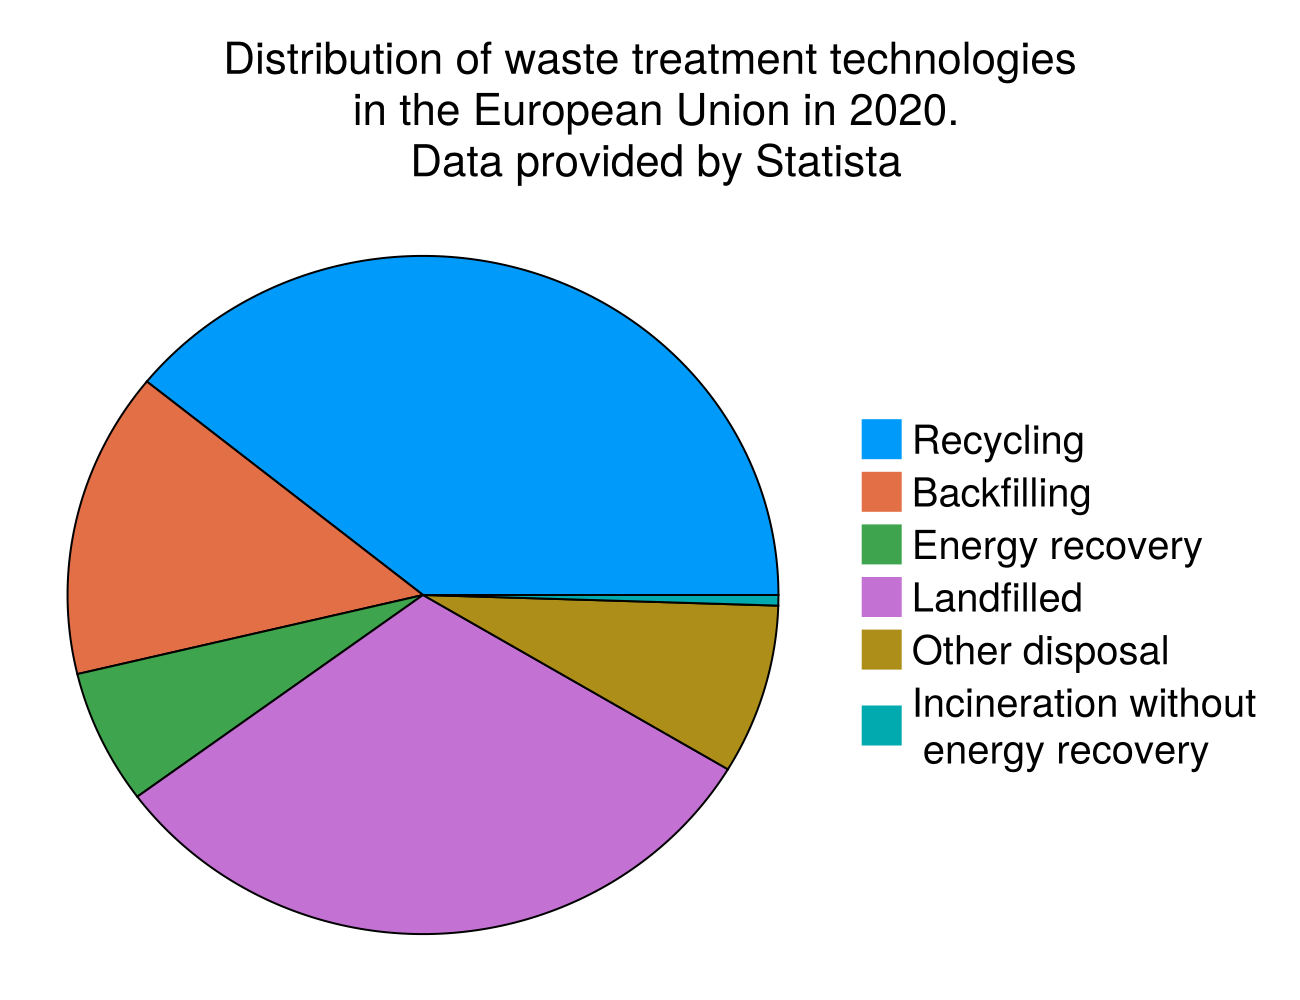
\includegraphics[width=.9\linewidth]{../plots/statistics/waste_treatment_technology_dist.png}
\caption[Τεχνολογίες επεξεργασίας απορριμμάτων στην Ευρωπαική Ένωση]{\label{fig:org9b00803}Τεχνολογίες επεξεργασίας απορριμμάτων στην Ευρωπαική Ένωση \textsuperscript{\citeprocitem{3}{3}}}
\end{figure}

Οι τεχνολογίες αυτές χρησιμοποιούνται επειδή είναι πολύ απλές και έχουν χαμηλό κόστος. Στα πλαίσια όμως της βιώσιμης ανάπτυξης και της κυκλικής οικονομίας, πρέπει τα απορρίμματα να εξετάζονται ως μία νέα πρώτη ύλη, από την οποία μπορούν να διυλιστούν προϊόντα αυξημένης αξίας.

Αυτές οι τεχνολογίες μπορεί να είναι θερμικές, όπως η πυρόλυση \textsuperscript{\citeprocitem{4}{4},\citeprocitem{5}{5}} η οποία παράγει ένα προϊόν γνωστό ως biochar, το οποίο έχει πολύ χρήσιμες ιδιότητες \textsuperscript{\citeprocitem{6}{6},\citeprocitem{7}{7}}, ή η αεριοποίηση \textsuperscript{\citeprocitem{5}{5},\citeprocitem{8}{8}}, η οποία παράγει ένα μίγμα υδρογόνου και μονοξειδίου του άνθρακα γνωστό ως \acrfull{syngas}, το οποίο μπορεί να χρησιμοποιηθεί ως πρώτη ύλη για πολλά προϊόντα. Στο \figurename \ref{fig:org2974f77} φαίνονται κάποια κλασσικά παραδείγματα αυτού \textsuperscript{\citeprocitem{9}{9}}

\begin{figure}[htbp]
\centering
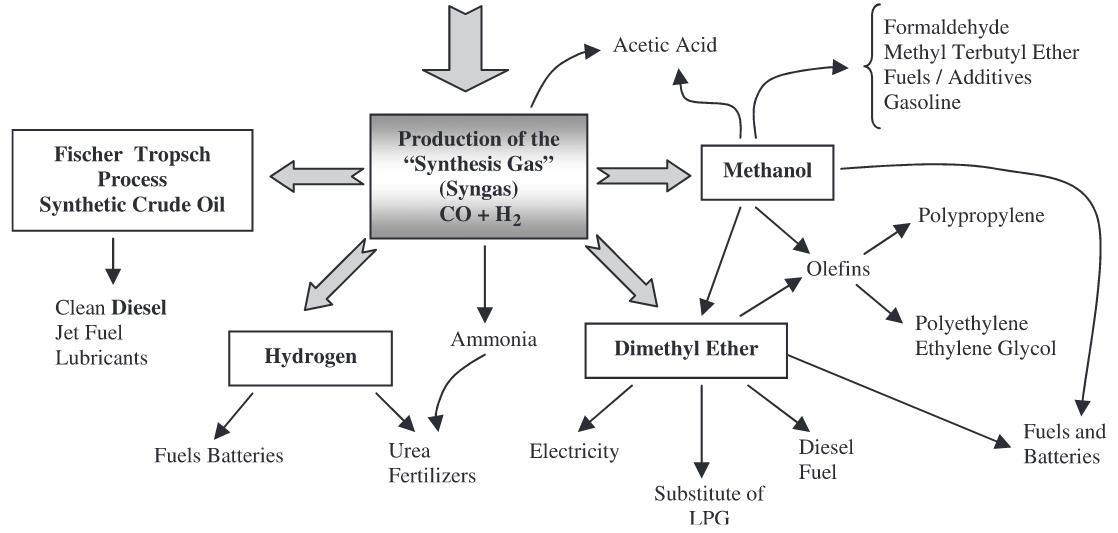
\includegraphics[width=.9\linewidth]{./gasification_products.jpg}
\caption[Προιόντα του αερίου σύνθεσης]{\label{fig:org2974f77}Προιόντα του αερίου σύνθεσης \textsuperscript{\citeprocitem{9}{9}}}
\end{figure}

Εκτός από θερμικές τεχνολογίες, υπάρχει μεγάλο ενδιαφέρον στις βιολογικές τεχνολογίες. Αυτές μπορεί να είναι αερόβιες, όπως η κομποστοποίηση, η οποία παράγει ένα εδαφοβελτιωτικό προϊόν \textsuperscript{\citeprocitem{10}{10}}, ή αναερόβιες όπως η αναερόβια χώνευση, η οποία έχει ως κύριο προϊόν το βιοαέριο, ένα μείγμα μεθανίου και διοξειδίου του άνθρακα που μπορεί να χρησιμοποιηθεί ως βιοκαύσιμο \textsuperscript{\citeprocitem{11}{11},\citeprocitem{12}{12}}, ή διάφορες διεργασίες ζύμωσης. Σε αυτές υπάγονται η αλκοολική ζύμωση, μία από τις πιο ευρέως χρησιμοποιούμενες τεχνολογίες αξιοποίησης απορριμμάτων \textsuperscript{\citeprocitem{13}{13},\citeprocitem{14}{14}}, η σκοτεινή ζύμωση για την παραγωγή υδρογόνου \textsuperscript{\citeprocitem{15}{15},\citeprocitem{16}{16}}, ή οι ζυμώσεις με σκοπό την παραγωγή μονομερών για βιοπολυμερή όπως το \acrfull{pla} \textsuperscript{\citeprocitem{17}{17},\citeprocitem{18}{18}} .

Η παρούσα μελέτη θα εστιάσει στην \acrfull{ad}, καθώς είναι μία τεχνολογία με μεγάλο δείκτη ετοιμότητας \acrfull{trl} \textsuperscript{\citeprocitem{19}{19}}, η οποία έχει εφαρμοστεί επιτυχώς σε μεγάλη κλίμακα, είναι οικονομική και φιλική προς το περιβάλλον \textsuperscript{\citeprocitem{20}{20}} .

Η \acrshort{ad} είναι μία αναερόβια βιολογική διεργασία η οποία διακρίνεται σε 4 στάδια. Στο πρώτο στάδιο, το αρχικό υπόστρωμα της διεργασίας, το οποίο συχνά αποτελείται από περίπλοκα πολυμερή όπως οι υδατάνθρακες, οι πρωτεΐνες και τα λιπίδια, υδρολύονται σε απλούστερες ενώσεις. Αυτές μπορούν να χρησιμοποιηθούν από τα οξεογόνα βακτήρια τα οποία τα μετατρέπουν σε \acrfull{vfa} όπως το οξικό οξύ, το προπιονικό οξύ, το βουτυρικό οξύ ή το γαλακτικό οξύ και σε αλκοόλες όπως η αιθανόλη. Στο 3ο στάδιο, οι ενώσεις αυτές μετατρέπονται σε οξικό οξύ, υδρογόνο και διοξείδιο του άνθρακα κατά την διεργασία της οξικογένεσης, ενώ τελικά, το οξικό οξύ μετατρέπεται σε μεθάνιο από μία κατηγορία μεθανογόνων μικροοργανισμών ενώ το υδρογόνο και το διοξείδιο του άνθρακα μετατρέπονται σε μεθάνιο από μία άλλη κατηγορία μεθανογόνων. Τα στάδια αυτά φαίνονται και στο \figurename \ref{fig:org5f295ea} \textsuperscript{\citeprocitem{21}{21}} .

\begin{figure}[htbp]
\centering
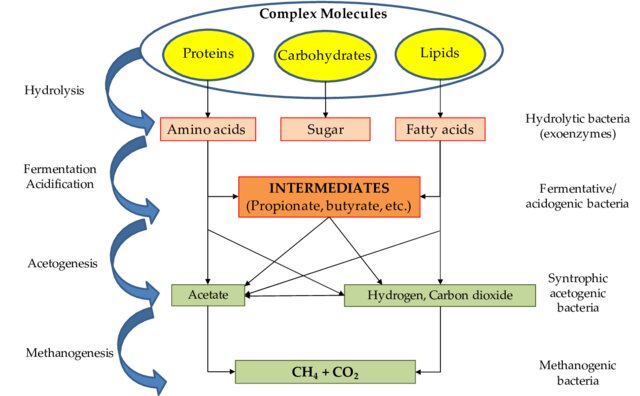
\includegraphics[width=280px]{./anaerobic_digestion_phases.jpg}
\caption[Φάσεις της αναερόβιας χώνευσης]{\label{fig:org5f295ea}Φάσεις της αναερόβιας χώνευσης \textsuperscript{\citeprocitem{21}{21}}}
\end{figure}

Ακόμη, είναι μία πολύ καλή τεχνολογία για την αξιοποίηση των \acrshort{fw} καθώς είναι πλούσια σε οργανική ύλη, η οποία είναι εύκολα αποδομήσιμη αλλά και σε θρεπτικά στοιχεία όπως το άζωτο, με υψηλότερο C/N από πολλά υποστρώματα. Λόγω αυτών, μπορούν να μετατραπούν πολύ αποτελεσματικά σε βιοαέριο \textsuperscript{\citeprocitem{11}{11}}.

Επιπροσθέτως, η \acrshort{ad} λύνει και άλλο ένα από τα σημαντικά προβλήματα του 21ου αιώνα, το οποίο είναι η ενέργεια. Αυτή τη στιγμή, πάνω από το \(80 \%\) της ενέργειας που καταναλώνεται παγκοσμίως βασίζεται σε μη ανανεώσιμες πηγές όπως το πετρέλαιο και το φυσικό αέριο. Οι ενεργειακές απαιτήσεις παγκοσμίως έχουν μία συνεχή αύξηση, ενώ οι πρώτες ύλες αυτές εξαλείφονται \textsuperscript{\citeprocitem{3}{3}} . Οπότε, τεχνολογίες παραγωγής ενέργειας από ανανεώσιμες πηγές, οι οποίες να έχουν το δυναμικό να αντικαταστήσουν τις πηγές αυτές, θα γίνουν απαραίτητες τα επόμενα χρόνια. Οι περισσότερες τεχνολογίες ανανεώσιμης ενέργειας (πχ αιολική, ηλιακή ή υδροηλεκτρική ενέργεια) έχουν δυσκολία να φτάσουν τέτοια επίπεδα και για αυτό χρησιμοποιούνται επικουρικά σε μία κύρια πηγή ενέργειας (αυτή τη στιγμή, περίπου το \(30 \%\) της παγκόσμιας παραγωγής ηλεκτρισμού οφείλεται σε τέτοιες πηγές) \textsuperscript{\citeprocitem{3}{3}} . Τα υπολείμματα τροφών από την άλλη είναι άφθονα οπότε θεωρείται πως με μία αποτελεσματική επεξεργασία θα μπορέσουν να καλύψουν ένα πολύ σημαντικό ποσοστό της παγκόσμιας ανάγκης σε ενέργεια.

Στο \figurename \ref{fig:orgb19c5e4} φαίνεται η παγκόσμια παραγωγή ενέργειας από βιοαέριο τα τελευταία 15 χρόνια, η οποία έχει ραγδαία αύξηση \textsuperscript{\citeprocitem{3}{3}} .

\begin{figure}[htbp]
\centering
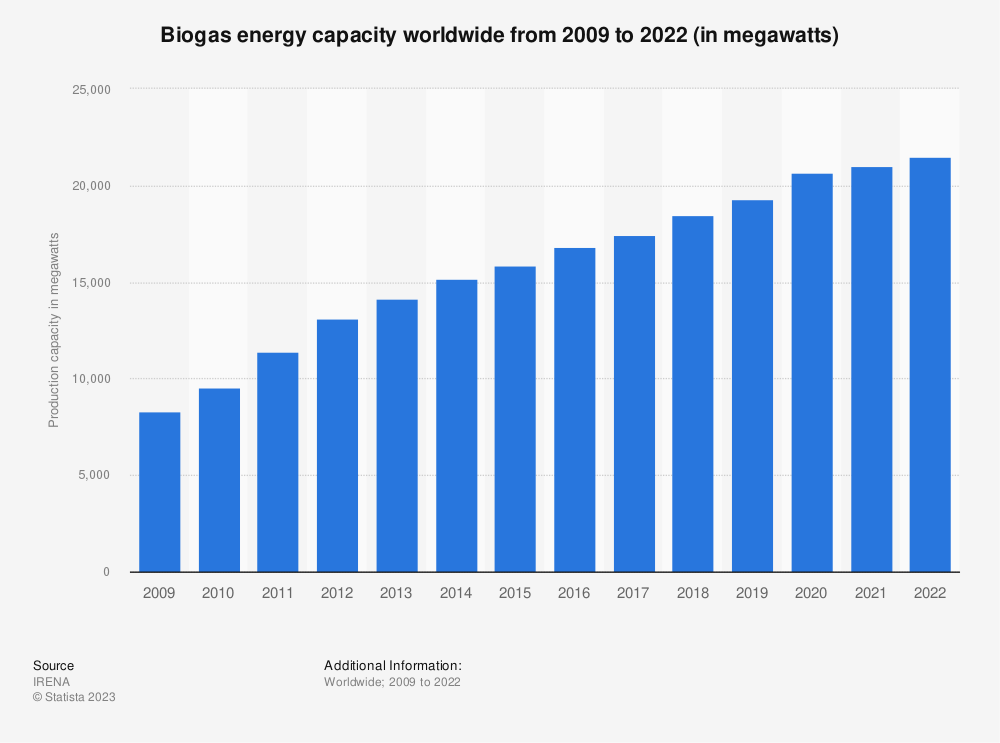
\includegraphics[width=.9\linewidth]{../plots/statistics/statistic_id1032922_global-biogas-energy-capacity-2009-2022.png}
\caption[Παγκόσμια παραγωγή ενέργειας από βιοαέριο]{\label{fig:orgb19c5e4}Παγκόσμια παραγωγή ενέργειας από βιοαέριο \textsuperscript{\citeprocitem{3}{3}}}
\end{figure}

Βέβαια, η \acrshort{ad} έχει και κάποια σημαντικά προβλήματα. Ο βασικός περιορισμός της είναι η ευαισθησία των μεθανογόνων μικροοργανισμών στις περιβαλλοντικές συνθήκες. Λόγω της ευαισθησίας τους, η \acrshort{ad} λειτουργεί στις βέλτιστες συνθήκες αυτών. Αυτό όμως οδηγεί στην λιγότερο αποτελεσματική διεξαγωγή των άλλων σταδίων. Το κυριότερο πρόβλημα που δημιουργείται είναι πως η υδρόλυση μπορεί μεν να διεξαχθεί, αλλά γίνεται σε πολύ αργό ρυθμό, καθιστώντας την το περιοριστικό στάδιο της \acrshort{ad} και τον λόγο για τον οποίο θεωρείται μία αρκετά αργή διεργασία. Ένα αντίστοιχο πρόβλημα υπάρχει και στο στάδιο της οξεογένεσης, όπου οι μικροοργανισμοί δεν λειτουργούν στις βέλτιστες συνθήκες τους και μπορούν να ακολουθήσουν μόνο ένα μεταβολικό μονοπάτι, το οποίο ενεργοποιείται στις συνθήκες που λειτουργούν. Έτσι, η οξεογένεση είναι πιθανόν να μην είναι ιδιαίτερα αποδοτική. Παρόλα αυτά, σε ορισμένες περιπτώσεις, ο ρυθμός της οξεογένεσης ξεπερνάει αυτόν της μεθανογένεσης (ο οποίος είναι γενικά αργός), με αποτέλεσμα να παράγονται υπερβολικές ποσότητες από \acrshort{vfa}, το οποίο οδηγεί σε οξίνιση του αντιδραστήρα και κατάρρευση της διεργασίας καθώς οι μεθανογόνοι δεν μπορούν να λειτουργήσουν σε εκείνες τις τιμές pH \textsuperscript{\citeprocitem{5}{5},\citeprocitem{22}{22},\citeprocitem{23}{23}}.

Ένας τρόπος να επιλυθεί το πρόβλημα αυτό είναι ο διαχωρισμός των σταδίων της υδρόλυσης και της ζύμωσης, σε μία διεργασία δύο \textsuperscript{\citeprocitem{24}{24}} ή τριών \textsuperscript{\citeprocitem{25}{25}} σταδίων. Αυτό που πετυχαίνεται με τον διαχωρισμό αυτόν είναι να λειτουργούν όλα τα στάδια της διεργασίας στο βέλτιστο σημείο λειτουργίας τους και άρα να είναι πολύ πιο αποτελεσματικά. Επιπροσθέτως, ο αντιδραστήρας δεν οξινίζεται κατά την διάρκεια της μεθανογένεσης, με αποτέλεσμα η διεργασία να είναι πολύ πιο σταθερή. Όμως, υπάρχει το πρόβλημα πως οι διεργασίες αυτές έχουν υψηλότερο κόστος, λόγω του περισσότερου εξοπλισμού, αλλά και πολυπλοκότητας της διεργασίας. Για τον λόγο αυτόν, η διεργασία αναερόβιας χώνευσης πολλαπλών σταδίων έχει πολύ χαμηλότερο \acrshort{trl} και δεν έχει εφαρμοστεί ευρέως σε μεγάλη κλίμακα \textsuperscript{\citeprocitem{5}{5},\citeprocitem{11}{11},\citeprocitem{22}{22},\citeprocitem{26}{26}} .

Η υδρόλυση αποτελεί σημαντικό στάδιο της επεξεργασίας \acrshort{fw}, καθώς έχουν υψηλή περιεκτικότητα σε βιοπολυμερή. Αυτή μπορεί να γίνει θερμικά, μηχανικά, χημικά ή ενζυμικά \textsuperscript{\citeprocitem{11}{11},\citeprocitem{27}{27},\citeprocitem{28}{28}}. Συνήθως η υδρόλυση γίνεται ενζυμικά καθώς έχει καταγραφεί πως επιφέρει τις υψηλότερες αποδόσεις και δεν παράγει προϊόντα τοξικά για τους μικροοργανισμούς. Ακόμη, είναι η μόνη που μπορεί να γίνει παράλληλα με την οξεογένεση για την περίπτωση της αναερόβιας χώνευσης σε 2 στάδια \textsuperscript{\citeprocitem{11}{11},\citeprocitem{29}{29},\citeprocitem{30}{30}} . Παρόλα αυτά, το υψηλό κόστος των ενζυμικών σκευασμάτων καθιστά αυτή την τεχνολογία απαγορευτική σε μεγάλη κλίμακα. Για αυτό, υπάρχει αρκετή έρευνα γύρω από τεχνολογίες μείωσης του κόστους της ενζυμικής υδρόλυσης για την πιο αποτελεσματική λειτουργία της διεργασίας αυτής \textsuperscript{\citeprocitem{18}{18},\citeprocitem{31}{31}–\citeprocitem{33}{33}}. Μια υποσχόμενη και οικονομική λύση είναι η χρήση σκευασμάτων τα οποία περιέχουν ένζυμα αλλά και μικροοργανισμούς. Αυτά τα σκευάσματα επιτρέπουν την αποτελεσματική υδρόλυση των \acrshort{fw} αλλά ταυτόχρονα και μία ζύμωση για παραγωγή χρήσιμων προϊόντων, όπως η αιθανόλη και τα \acrshort{vfa}. Αυτά μπορούν να ανακτηθούν ως έχουν, ή να χρησιμοποιηθούν σε διάφορες βιοδιεργασίες, όπως η \acrshort{ad}. Ένα τέτοιο υπόστρωμα μπορεί να βελτιώσει την σταθερότητα μίας αναερόβιας χώνευσης αφού περιορίζονται τα στάδια της υδρόλυσης και οξεογένεσης και ευνοείται η δράση των μεθανογόνων μικροοργανισμών \textsuperscript{\citeprocitem{5}{5}}.

Ο σκοπός της παρούσας μελέτης είναι αρχικά να κάνει μία βιβλιογραφική ανασκόπηση των τεχνολογιών \acrshort{ad} σε πολλαπλά στάδια. Με βάση αυτήν θα αναπτυχθεί μία διεργασία αξιοποίησης υπολειμμάτων τροφών, αξιοποιώντας ένα \acrfull{mix}, η οποία να είναι οικονομικά βιώσιμη αλλά ταυτόχρονα αποτελεσματική. Αρχικά, θα αξιολογηθεί η ποιότητα της υδρόλυσης καθώς και της οξεογένεσης κατά την διεργασία αυτή σε εργαστηριακή κλίμακα, όπου υπάρχει καλός έλεγχος παραμέτρων όπως η θερμοκρασία και η ποσότητα του \acrshort{mix}. Έπειτα, θα εξεταστεί η κλιμάκωση της διεργασίας σε πιλοτική κλίμακα εξετάζοντας την ποσότητα του \acrshort{mix} και την παροχή νερού ως λειτουργικές παραμέτρους. Τέλος, θα διερευνηθεί η δυνατότητα αξιοποίησης της παραγόμενης υγρής εκροής για την παραγωγή μεθανίου σε αναερόβιους αντιδραστήρες εργαστηριακής κλίμακας.

Η δομή της εργασίας θα είναι ως εξής: Στην συνέχεια του πρώτου μέρους θα γίνει η βιβλιογραφική ανασκόπηση, η οποία θα χωριστεί σε 5 κεφάλαια. Αρχικά, στο \autoref{sec:anaerobic_digestion} θα γίνει μία πιο αναλυτική παρουσίαση της \acrshort{ad} και των προβλημάτων που δημιουργούνται αν όλα τα στάδια αυτής γίνονται ταυτόχρονα. Σκοπός αυτού είναι η ανάδειξη της σημασίας της \acrshort{ad} σε πολλαπλά στάδια. Έτσι, τα επόμενα κεφάλαια θα εστιάσουν στα στάδια της \acrshort{ad} αν αυτά διεξαχθούν ξεχωριστά. Στο \autoref{sec:fw_pretreatment} θα αναλυθούν όλες οι μέθοδοι προ-επεξεργασίας υπολειμμάτων τροφών που έχουν βρεθεί στην βιβλιογραφία για να υδρολύσουν πιο αποτελεσματικά τα \acrshort{fw}, με τα πλεονεκτήματα και τα μειονεκτήματα τους, ενώ στο \autoref{sec:enzymes} θα δοθεί ιδιαίτερη έμφαση στην ενζυμική υδρόλυση, και στις προσπάθειες μείωσης του κόστους αυτής. Το \autoref{sec:acidogenesis} θα εστιάσει στην οξεογένεση και θα αναφέρει όλα τα διαθέσιμα μεταβολικά μονοπάτια αυτής και πως καθορίζεται ποιο θα επικρατήσει με βάση τις λειτουργικές συνθήκες. Ακόμη, θα αναφερθεί η χρησιμότητα του κάθε μεταβολικού προϊόντος για την \acrshort{ad} για να αποφανθεί το βέλτιστο μονοπάτι. Τέλος, στο \autoref{sec:methanogenesis} θα μελετηθούν η οξικογένεση και η μεθανογένεση. Τα 2 αυτά στάδια δεν θα διαχωριστούν, καθώς στην πράξη, το ένα εξαρτάται από το άλλο και γίνονται συνεργιστικά.

Έχοντας τις πληροφορίες αυτές, μπορεί στο δεύτερο μέρος, να γίνει μία ανάλυση των πειραματικών αποτελεσμάτων της εργασίας και να προκύψουν κάποια συμπεράσματα από αυτά. Συγκεκριμένα, στο \autoref{sec:materials_methods} θα αναλυθούν οι πειραματικές διαδικασίες που χρησιμοποιήθηκαν καθώς και οι πρώτες ύλες που χρειάστηκαν. Στο \autoref{sec:result_analysis} θα αναφερθούν τα πρωτογενή αποτελέσματα κάθε πειραματικός κύκλου, αλλά και πως αυτά αναλύθηκαν με σκοπό στο \autoref{sec:result_discussion} να γίνει μία συζήτηση των αποτελεσμάτων αυτών καθώς και η παράθεση κάποιων συγκριτικών αποτελεσμάτων, από τα οποία θα προκύψουν άμεσα και τα συμπεράσματα της εργασίας, τα οποία θα παρατεθούν στο \autoref{sec:conclusion} μαζί με κάποιες προτάσεις για περαιτέρω έρευνα στο αντικείμενο αυτό.

\chapter{Αναερόβια Χώνευση}
\label{sec:org721740a}
\label{sec:anaerobic_digestion}

Η αναερόβια χώνευση είναι μία αναερόβια βιολογική διεργασία η οποία μετατρέπει περίπλοκη οργανική ύλη σε μεθάνιο και διοξείδιο του άνθρακα με βάση τον μηχανισμό του σχήματος \ref{fig:org5f295ea}. Η διεργασία αυτή έχει πολλά πλεονεκτήματα, όπως η απλότητα της λειτουργίας, το χαμηλό σχετικά λειτουργικό κόστος (χρειάζεται μόνο η διατήρηση της θερμοκρασίας σε ένα σταθερό επίπεδο) και την παραγωγή ενός πολύ αποτελεσματικού ενεργειακού φορέα, του μεθανίου \textsuperscript{\citeprocitem{27}{27}}. Για αυτούς τους λόγους μάλιστα έχει δει ραγδαία ανάπτυξη τα τελευταία χρόνια \textsuperscript{\citeprocitem{3}{3}} .

Όμως, παραμένει περιορισμένη σε μεγάλο βαθμό από τα λειτουργικά της προβλήματα \textsuperscript{\citeprocitem{27}{27}}. Αρχικά, είναι μία αργή διεργασία. Αυτό οφείλεται εν μέρει στους μεθανογόνους μικροοργανισμούς, οι οποίοι θέλουν ο \acrfull{hrt} να είναι μεγάλος για να μπορέσουν να αναπτυχθούν και να μην εκπλυθούν. Αλλά, για τα περισσότερα υποστρώματα, το περιοριστικό στάδιο της διεργασίας είναι η υδρόλυση και διαλυτοποίηση, δηλαδή η διάσπαση των στερεών και μακρομερών σωματιδίων σε διαλυτές ενώσεις, οι οποίες μπορούν να μεταβολιστούν. Στην περίπτωση των υπολειμμάτων τροφών, ένα μεγάλο ποσό της οργανικής ύλης βρίσκεται σε σωματιδιακή μορφή και δεν είναι διαλυτό. Είναι στην πλειοψηφία του ένα εύκολα υδρολύσιμο υπόστρωμα, αλλά αν η υδρόλυση γίνει κατά την διάρκεια της χώνευσης, επιβραδύνει τον χρόνο που διαρκεί η χώνευση \textsuperscript{\citeprocitem{5}{5},\citeprocitem{11}{11},\citeprocitem{28}{28}} . Αυτό γίνεται επειδή κατά την λειτουργία ενός χωνευτήρα, οι λειτουργικές συνθήκες ρυθμίζονται στις βέλτιστες των μεθανογόνων μικροοργανισμών, οι οποίοι είναι οι πιο ευαίσθητοι. Αυτές είναι συνήθως στη μεσόφιλη περιοχή της θερμοκρασίας (35-37 \(^oC\)) και σε pH κοντά στο ουδέτερο (6.4-8.0). Αντιθέτως, η βέλτιστη λειτουργία της υδρόλυσης από τους ήδη υπάρχοντες μικροοργανισμούς στην λάσπη είναι βέλτιστη σε πολύ πιο όξινα pH \textsuperscript{\citeprocitem{25}{25},\citeprocitem{34}{34}} και τα συνήθη υδρολυτικά ένζυμα που εκκρίνονται από τους μικροοργανισμούς αυτούς λειτουργούν βέλτιστα σε υψηλότερες θερμοκρασίες \textsuperscript{\citeprocitem{11}{11},\citeprocitem{29}{29},\citeprocitem{35}{35}} . Για τους λόγους αυτούς, είναι συχνό να γίνεται κάποια προ-επεξεργασία πριν την αναερόβια χώνευση, η οποία αποσκοπεί στην υδρόλυση και διαλυτοποίηση του υποστρώματος \textsuperscript{\citeprocitem{11}{11},\citeprocitem{27}{27},\citeprocitem{36}{36},\citeprocitem{37}{37}} .

Το άλλο βασικό πρόβλημα της αναερόβιας χώνευσης, είναι η ανισορροπία στους ρυθμούς της αντίδρασης. Στην περίπτωση που και τα 4 στάδια γίνονται ταυτόχρονα, μία ευσταθής συνθήκη λειτουργίας, θα ήταν όλα τα στάδια να έχουν τον ίδιο ρυθμό, ώστε ότι παράγεται να καταναλώνεται. Στην πράξη όμως, αυτό δεν συμβαίνει. Οι οξεογόνοι μικροοργανισμοί συχνά μεταβολίζουν το υπόστρωμα τους πιο γρήγορα από τους μεθανογόνους, οπότε σε πολλές περιπτώσεις μπορεί να παρατηρηθεί συσσώρευση πτητικών λιπαρών οξέων. Η συσσώρευση αυτή σημαίνει πως θα μειωθεί το pH του αντιδραστήρα σε ένα επίπεδο που θα ανασχεθεί η λειτουργία των μεθανογόνων μικροοργανισμών και σταδιακά θα σταματήσει η παραγωγή μεθανίου, κάτι που θα συντελέσει στην κατάρρευση του συστήματος. Η ανισορροπία αυτή στους ρυθμούς μπορεί όμως να συντελέσει και άλλο ένα πρόβλημα. Εκτός από \acrshort{vfa}, παράγεται και υδρογόνο κατά την οξεογένεση. Η υψηλή μερική πίεση υδρογόνου στο σύστημα είναι επίσης ανασχετική για τους μεθανογόνους και μπορεί να οδηγήσει το σύστημα σε κατάρρευση. Λόγω των προβλημάτων αυτών, το σύστημα αναερόβιας χώνευσης ενός σταδίου, δεν έχει ιδιαίτερα μεγάλη σταθερότητα \textsuperscript{\citeprocitem{12}{12},\citeprocitem{22}{22},\citeprocitem{25}{25},\citeprocitem{27}{27}} .

Ο συμβατικός τρόπος που επιλύεται αυτό είναι o χαμηλός \acrfull{olr}. Αν το σύστημα τροφοδοτείται με μικρή ποσότητα υποστρώματος, θα είναι χαμηλός γενικά ο ρυθμός της οξεογένεσης, με αποτέλεσμα να είναι πιο δύσκολο να δημιουργηθεί αστάθεια. Βέβαια, η χρήση πολύ χαμηλού \acrshort{olr} είναι προβληματική επειδή περιορίζει σημαντικά τον ρυθμό επεξεργασίας του αποβλήτου. Ειδικά στην περίπτωση των υπολειμμάτων τροφών τα οποία παράγονται σε πολύ μεγάλους ρυθμούς, θα ήταν ιδανικό ο χωνευτήρας να λειτουργεί σε υψηλό ρυθμό οργανικής φόρτισης. Ένας τρόπος να αυξηθεί ο \acrshort{olr} είναι η χρήση ενός ταχύρυθμου αντιδραστήρα όπως ο \acrfull{uasb}. Στον αντιδραστήρα αυτόν, η λάσπη που δημιουργείται είναι κοκκώδης και παρατηρείται σχηματισμός βιοφίλμ. Έτσι, ο κάθε κόκκος αποτελεί ένα μικροβιακό οικοσύστημα όπου οι πιο ευαίσθητοι μικροοργανισμοί, όπως οι μεθανογόνοι προστατεύονται από τις εξωτερικές συνθήκες. Αυτό έχει ως αποτέλεσμα η διεργασία να έχει μεγαλύτερη σταθερότητα και να μπορεί να διεξαχθεί πιο γρήγορα. Αυτό επιτρέπει και την αύξηση του \acrshort{olr} \textsuperscript{\citeprocitem{22}{22},\citeprocitem{26}{26},\citeprocitem{38}{38}} .

Όμως, ο πιο αποτελεσματικός τρόπος να αυξηθεί ο \acrlong{olr} σε έναν αντιδραστήρα αναερόβιας χώνευσης είναι μία διάταξη σε δύο στάδια \textsuperscript{\citeprocitem{22}{22}–\citeprocitem{24}{24}}. Σε αυτή, διαχωρίζονται τα στάδια της υδρόλυσης και οξεογένεσης από την μεθανογένεση. Ως αποτέλεσμα, η εκροή του οξεογενή αντιδραστήρα μπορεί να υποστεί μία ρύθμιση pH στην περιοχή που λειτουργούν βέλτιστα οι μεθανογόνοι και εφόσον έχει ολοκληρωθεί ήδη η οξεογένεση, δεν υπάρχει ο κίνδυνος να οξινιστεί ο αντιδραστήρας, κάτι που θα οδηγούσε στην κατάρρευση του. Έτσι, τα συστήματα αυτά είναι πολύ πιο σταθερά και μπορούν να λειτουργήσουν σε μεγαλύτερα \acrshort{olr} πολύ αποτελεσματικά \textsuperscript{\citeprocitem{24}{24},\citeprocitem{26}{26}}. Ακόμη ένα πλεονέκτημα της διάταξης αυτής είναι πως διαχωρίζοντας τα στάδια της υδρόλυσης και της οξεογένεσης, το οποίο επιτρέπει την λειτουργία τους σε πιο επιθυμητές συνθήκες. Η οξεογένεση είναι μία περίπλοκη διεργασία η οποία μπορεί να ακολουθήσει πολλά μεταβολικά μονοπάτια ανάλογα με τις συνθήκες στις οποίες θα διεξαχθεί. Η επιλογή του βέλτιστου μονοπατιού εξαρτάται από πολλούς παράγοντες και θα αναλυθεί περαιτέρω στο \autoref{sec:acidogenesis}, αλλά είναι κάτι που είναι εφικτό μόνο σε συστήματα δύο φάσεων. Η βέλτιστη λειτουργία της υδρόλυσης είναι λίγο πιο καθορισμένη. Όμως, συνήθως δεν λαμβάνεται υπόψιν στα συστήματα δύο φάσεων, καθώς συνήθως καθορίζονται από την οξεογένεση. Καθώς η υδρόλυση λειτουργεί βέλτιστα σε όξινα pH, η λειτουργία της στο σύστημα αυτό είναι σίγουρα πιο αποτελεσματική από την υδρόλυση στο σύστημα μίας φάσης \textsuperscript{\citeprocitem{5}{5},\citeprocitem{11}{11},\citeprocitem{22}{22},\citeprocitem{26}{26}}. Στην βιβλιογραφία, υπάρχουν και κάποια συστήματα αναερόβιας χώνευσης τριών σταδίων \textsuperscript{\citeprocitem{5}{5},\citeprocitem{25}{25},\citeprocitem{34}{34},\citeprocitem{39}{39}}, στα οποία λειτουργεί και η υδρόλυση ξεχωριστά και στο βέλτιστο σημείο λειτουργίας της. Η διεργασία αυτή είναι πιο αποτελεσματική και πιο σταθερή, αλλά ταυτόχρονη ακόμη πιο περίπλοκη. Οπότε, γενικά προτιμάται η διεργασία δύο σταδίων, ως μία ισορροπία μεταξύ πολυπλοκότητας και σταθερότητας της λειτουργίας \textsuperscript{\citeprocitem{5}{5}}.

\chapter{Προεπεξεργασία Υπολειμμάτων Τροφών}
\label{sec:orga79efe2}
\label{sec:fw_pretreatment}

Τα \acrshort{fw} έχουν υψηλή περιεκτικότητα σε βιοπολυμερή. Για να μπορέσουν να χρησιμοποιηθούν αποδοτικά ως ένα υπόστρωμα για διεργασίες όπως η \acrshort{ad}, απαιτείται κάποια διεργασία η οποία θα υδρολύσει το υπόστρωμα αυτό. Υπάρχουν πολλές τεχνολογίες για να βοηθήσουν την υδρόλυση του υποστρώματος αυτού όπως η μηχανική, θερμική, χημική ή ενζυμική προεπεξεργασία και η προ-επεξεργασίες με υπερήχους και μικροκύματα.

\section{Μηχανική Επεξεργασία}
\label{sec:org4756e93}
Η πιο απλή είναι η μηχανική επεξεργασία. Μία μηχανική επεξεργασία όπως ο τεμαχισμός είναι αρκετά αποτελεσματική. Ο σκοπός της είναι η ομογενοποίηση της στερεής μάζας και μείωση του μεγέθους κόκκων της ώστε να επιταχυνθούν τα επόμενα στάδια της προ-επεξεργασίας. Είναι το πιο σύνηθες στάδιο προ-επεξεργασίας και γίνεται ανεξαρτήτως των επόμενων σταδίων συνήθως \textsuperscript{\citeprocitem{5}{5},\citeprocitem{40}{40},\citeprocitem{41}{41}} . 

\section{Θερμική Επεξεργασία}
\label{sec:orgd8a4f3a}
Η θερμική υδρόλυση βασίζεται στην αύξηση της θερμοκρασίας, με σκοπό την διάσπαση των πολυμερικών δεσμών. Είναι πολύ αποτελεσματική ως μία προ-επεξεργασία για δύσκολα αποδομήσιμη βιομάζα. Στην περίπτωση των \acrshort{fw}, οι υψηλές θερμοκρασίες δεν είναι αναγκαίες για την αποικοδόμηση και μάλιστα συνήθως υποβαθμίζουν την ποιότητα του υποστρώματος καθώς καταστρέφουν οργανική ύλη και μπορεί να παράξουν προϊόντα θερμικής αποδόμησης τα οποία είναι τοξικά για επόμενα βιολογικά στάδια. Ακόμη, είναι μία τεχνική με σχετικά υψηλές ενεργειακές απαιτήσεις \textsuperscript{\citeprocitem{11}{11},\citeprocitem{27}{27},\citeprocitem{36}{36}} .

\section{Επεξεργασία με Μικροκύματα}
\label{sec:org2823158}
Αντίστοιχη λογική έχει και η χρήση μικροκυμάτων, η οποία αυξάνει την θερμοκρασία μέσω ενός ηλεκτρομαγνητικού πεδίου. Θεωρείται πιο αποτελεσματική από την θερμική τεχνολογία λόγω της μικρότερης κατανάλωσης ενέργειας. Επίσης, συνδυάζει θερμικά με μη θερμικά φαινόμενα. Όμως, όπως και στη περίπτωση της θερμικής υδρόλυσης, δεν επιφέρει ιδιαίτερα θετικά αποτελέσματα για την επεξεργασία \acrshort{fw} \textsuperscript{\citeprocitem{11}{11},\citeprocitem{27}{27},\citeprocitem{36}{36}} . 

\section{Επεξεργασία με Υπερήχους}
\label{sec:orgf9fe366}
Η χρήση υπερήχων βασίζεται στην δημιουργία ελεύθερων ριζών υδροξυλίου \(OH^{\cdot}\), οι οποίες διασπούν ταχύτατα τα στερεά, απελευθερώνοντας μεγάλα ποσά οργανικής ύλης. Πειράματα που έχουν χρησιμοποιήσει υπερήχους ως μία προ-επεξεργασία για αναερόβια χώνευση έχουν δείξει πως βελτιώνει αρκετά την παραγωγή μεθανίου. Βέβαια, υδρολύουν μόνο σε περιορισμένο βαθμό το υπόστρωμα, με αποτέλεσμα να πρέπει να γίνει και κάποια υδρόλυση κατά την διάρκεια της χώνευσης \textsuperscript{\citeprocitem{11}{11},\citeprocitem{36}{36}} .

\section{Χημική Επεξεργασία}
\label{sec:org6b2e034}
Σε ένα παρόμοιο μηχανισμό βασίζεται και η χημική τεχνολογία της οζόνωσης, καθώς η τροφοδοσία με όζον δημιουργεί και αυτή ελεύθερες ρίζες οι οποίες διασπούν την στερεή οργανική ύλη. Είναι όμως μία πιο έντονη επεξεργασία η οποία χρησιμοποιείται σε υποστρώματα τα οποία είναι πιο δύσκολα στην αποδόμηση. Στην περίπτωση των \acrshort{fw} μπορεί να οδηγήσουν σε μείωση του COD λόγω οξείδωσης ακόμη και των ζυμώσιμων σακχάρων και παραγωγής προϊόντων πιο δύσκολα αποδομήσιμα από τα αρχικά, για αυτό αποφεύγεται \textsuperscript{\citeprocitem{27}{27},\citeprocitem{36}{36}} .

Βέβαια, η πιο συχνή κατηγορία χημικής επεξεργασίας είναι αυτή που βασίζεται στην προσθήκη οξέος ή βάσης. Η προσθήκη των ενώσεων αυτών βασίζεται στην επίτευξη ακραίων τιμών pH, στις οποίες καταρρέει η πολυμερική δομή. Στην τεχνολογία αυτή χρησιμοποιούνται ισχυρά οξέα ή βάσεις (πχ θειικό οξύ, υδροχλωρικό οξύ, καυστικό νάτριο ή ασβέστης). Η τεχνολογία αυτή είναι η πιο απλή και φθηνή τεχνολογία προ-επεξεργασίας, αλλά είναι και αρκετά αποτελεσματική. Για αυτό χρησιμοποιείται αρκετά \textsuperscript{\citeprocitem{11}{11},\citeprocitem{29}{29},\citeprocitem{36}{36}}. Ακόμη, για την αλκαλική υδρόλυση, ισχύει πως αν τα \acrshort{fw} χρησιμοποιηθούν μετά για αναερόβια χώνευση, το σύστημα θα έχει αποκτήσει μεγαλύτερη αλκαλικότητα, με αποτέλεσμα να έχει καλύτερη σταθερότητα η διεργασία \textsuperscript{\citeprocitem{27}{27}} . Όμως, μπορεί να παραχθούν μη επιθυμητά προϊόντα κατά την όξινη ή αλκαλική αποδόμηση των \acrshort{fw}, όπως η φουρφουράλη, τα οποία είναι τοξικά προς μικροοργανισμούς και άρα να μειωθεί σημαντικά η απόδοση της διεργασίας \textsuperscript{\citeprocitem{11}{11},\citeprocitem{29}{29},\citeprocitem{30}{30}} .

\section{Ενζυμική Επεξεργασία}
\label{sec:orgac881e5}
Τέλος, υπάρχει η ενζυμική επεξεργασία. Αυτή βασίζεται στην χρήση υδρολυτικών ενζύμων όπως οι υδατανθρακάσες, οι πρωτεάσες και οι λιπάσες για την διάσπαση των βιοπολυμερών. Η διεργασία αυτή δεν έχει κανένα τοξικό παραπροϊόν, ήπιες συνθήκες (οι οποίες συνδέονται με το κόστος) και εξαιρετική απόδοση υδρόλυσης/βιοαποδόμησης \textsuperscript{\citeprocitem{11}{11},\citeprocitem{30}{30},\citeprocitem{42}{42}}. Επίσης, είναι η μόνη προ-επεξεργασία, της οποίας οι συνθήκες μπορούν να ρυθμιστούν έτσι ώστε να γίνει ταυτόχρονα με την οξεογένεση, το οποίο επιτρέπει την αναερόβια χώνευση σε 2 στάδια. Σε κάθε άλλη περίπτωση, η διεργασία πρέπει να γίνει σε τρία στάδια, το οποίο παρότι προσφέρει σταθερότητα και πιθανόν καλύτερες αποδόσεις, δημιουργεί και πολυπλοκότητα στην διεργασία \textsuperscript{\citeprocitem{5}{5},\citeprocitem{11}{11}} . Παρόλα αυτά, το κόστος ενός εμπορικού ενζυμικού σκευάσματος είναι πολύ υψηλό, κάτι που καθιστά την συμβατική ενζυμική υδρόλυση μία τεχνολογία απαγορευτική σε μεγάλη κλίμακα. Για τον λόγο αυτόν, στην βιβλιογραφία υπάρχουν αρκετές μελέτες χρησιμοποιώντας πρωτοποριακές τεχνολογίες ενζυμικής υδρόλυσης χαμηλού κόστους για να λύσουν το πρόβλημα αυτό \textsuperscript{\citeprocitem{18}{18},\citeprocitem{25}{25},\citeprocitem{33}{33},\citeprocitem{43}{43},\citeprocitem{44}{44}} . Οι τεχνολογίες αυτές θα αναλυθούν σε περισσότερο βάθος στο \autoref{sec:enzymes}.

\section{Απόκριση της Υδρόλυσης}
\label{sec:org6f0be70}
Αλλά μία σημαντική ερώτηση που έγκειται για την υδρόλυση, είναι πως προσδιορίζεται πειραματικά η απόδοση μίας τέτοιας διεργασίας. Στην πράξη, το σημαντικότερο μέτρο για αυτό είναι ο λόγος \acrfull{scod} προς \acrfull{tcod}. Αυτό δείχνει πόση από την οργανική ύλη έχει διαλυτοποιηθεί και στα \acrshort{fw} ξεκινάει από \(20-30 \%\) συνήθως και μπορεί να φτάσει από \(60 - 80 \%\) σε μία αρκετά αποδοτική υδρόλυση \textsuperscript{\citeprocitem{28}{28},\citeprocitem{37}{37},\citeprocitem{45}{45}} .

\chapter{Βελτιστοποίηση της Διεργασίας της Ενζυμικής Υδρόλυσης}
\label{sec:orgaae4fa7}
\label{sec:enzymes}

Στο \autoref{sec:fw_pretreatment} αναφέρθηκαν όλες οι τεχνολογίες προ-επεξεργασίας των \acrshort{fw}. Σκοπός αυτών είναι η επίτευξη υψηλών αποδόσεων σε επόμενα βιολογικά στάδια όπως η \acrshort{ad}. Προέκυψε, πως η ενζυμική υδρόλυση/βιοαποδόμηση είναι η πιο αποτελεσματική καθώς δεν έχει παραπροϊόντα, χρησιμοποιεί ήπιες συνθήκες, μειώνει αποτελεσματικά τα \acrfull{ts} και αυξάνει το διαλυτό \acrfull{cod}, ενώ μπορεί να γίνει παράλληλα με την οξεογένεση. Όμως, αναφέρθηκε πως το κύριο εμπόδιο της είναι το κόστος των ενζυμικών σκευασμάτων. Για αυτό, στο κεφάλαιο αυτό θα αναφερθούν όλες οι τεχνολογίες που έχουν προταθεί στην βιβλιογραφία για την μείωση του κόστους της διεργασίας αυτής. Γενικά, κατατάσσονται σε δύο κατηγορίες:

\begin{itemize}
\item Εντατικοποίηση της διεργασίας υδρόλυσης (\acrfull{pi}) και μείωση του απαιτούμενου χρόνου υδρόλυσης, ο οποίος σε συνεχή συστήματα αντιστοιχεί στην ποσότητα ενζύμων που απαιτούνται.
\item Χρήση μικροοργανισμών, οι οποίοι στις κατάλληλες συνθήκες θα εκκρίνουν υδρολυτικά ένζυμα in-situ για την υδρόλυση
\end{itemize}

\section{Εντατικοποίηση της Διεργασίας Υδρόλυσης}
\label{sec:org480a07f}
Οι μελέτες οι οποίες υπάγονται σε αυτήν την κατηγορία αποτελούν τις μελέτες οι οποίες έχουν προσπαθήσει να βελτιστοποιήσουν διάφορες συνθήκες της υδρόλυσης, με σκοπό την πιο αποτελεσματική και γρήγορη ενζυμική υδρόλυση, η οποία θα έχει χαμηλότερο κόστος.

Για παράδειγμα, οι \textsuperscript{\citeprocitem{37}{37}} προσπάθησαν να μειώσουν πολύ τον χρόνο παραμονής στην υδρόλυση και έδειξαν ότι με βέλτιστες συνθήκες, σε περίπου 4 ώρες έχει γίνει ικανοποιητική υδρόλυση. Καθώς ο χρόνος αυτός συχνά είναι στις 24 ώρες, μία τέτοια μείωση θα μπορούσε να μειώσει σημαντικά την απαίτηση σε ένζυμα και άρα να βελτιώσει το οικονομικό προφίλ της διεργασίας \textsuperscript{\citeprocitem{11}{11},\citeprocitem{46}{46},\citeprocitem{47}{47}} .

Οι \textsuperscript{\citeprocitem{44}{44}} έκαναν μία μελέτη στην οποία προσπάθησαν να βελτιστοποιήσουν μία διεργασία παραγωγής βιοαιθανόλης από απόβλητα της βιομηχανίας επεξεργασίας πατάτας λαμβάνοντας υπόψιν συνθήκες όπως η ποσότητα ενζύμων που θα χρησιμοποιηθεί και η πιθανότητα χρήσης άλλων διεργασιών υδρόλυσης επικουρικά, όπως η προσθήκη HCl ή χρήση υπερήχων κατά την διεργασία.

Οι \textsuperscript{\citeprocitem{48}{48}} χρησιμοποίησαν έναν συνδυασμό υπερήχων και ενζυμικής υδρόλυσης με σκοπό οι υπέρηχοι να κάνουν την βιομάζα πιο προσβάσιμη στα ένζυμα, με σκοπό να μειωθεί σημαντικά η ποσότητα ενζύμων που πρέπει να προστεθεί. Η μελέτη τους έδειξε πως αυτός ο συνδυασμός είναι αρκετά αποτελεσματικός.

Παρόλο που υπήρχαν αρκετές επιτυχίες στον τομέα αυτόν, ακόμη και με σημαντική μείωση της ποσότητας ενζύμων που χρειάζονται, όσο μεγαλώνει η κλίμακα, γίνεται όλο και πιο δύσκολο η τεχνική αυτή να είναι αποτελεσματική. Οπότε, θεωρείται πως οι πιο αποτελεσματικές τεχνικές υδρόλυσης είναι στην δεύτερη κατηγορία, όπου το σύστημα τροφοδοτείται με μικροοργανισμούς και οι συνθήκες ελέγχονται ώστε να παραχθούν in-situ μεγάλες ποσότητες υδρολυτικών ενζύμων.

\section{Ζύμωση Στερεής Κατάστασης}
\label{sec:orgb036e35}
Η ζύμωση στερεής κατάστασης (\acrfull{ssf}) είναι μία αρκετά ενδιαφέρουσα κατηγορία ζύμωσης. Η βασική της αρχή είναι πως δεν χρησιμοποιείται νερό στον αντιδραστήρα όπου θα αναπτυχθεί ο μικροοργανισμός (ή οι μικροοργανισμοί στη περίπτωση μικτής καλλιέργειας) αλλά κάποια στερεή φάση, η οποία μπορεί να χρησιμοποιηθεί ως η τροφή του μικροοργανισμού \textsuperscript{\citeprocitem{18}{18},\citeprocitem{33}{33}}.

Μία από τις βασικές εφαρμογές της \acrshort{ssf} είναι η ανάπτυξη μυκήτων οι οποίοι μπορούν να εκκρίνουν μεγάλη ποσότητα ενζύμων. Η τεχνολογία αυτή για την παραγωγή υδρολυτικών ενζύμων έχει αρκετό ενδιαφέρον, καθώς είναι μία διεργασία η οποία χρησιμοποιεί συχνά απόβλητα ως πρώτη ύλη. Για παράδειγμα, μπορούν τα ίδια \acrshort{fw} που θα χρησιμοποιηθούν για την \acrshort{ad} να χρησιμοποιηθούν και στην \acrshort{ssf} \textsuperscript{\citeprocitem{49}{49}}. Έπειτα, η βιομάζα που έχει παραχθεί στην \acrshort{ssf} μπορεί να αναμειχθεί με τα υπόλοιπα \acrshort{fw} και το μείγμα αυτό να χρησιμοποιηθεί για διεργασίες όπως η αναερόβια χώνευση \textsuperscript{\citeprocitem{33}{33},\citeprocitem{50}{50}}. Ακόμη όμως και στην περίπτωση που δεν χρησιμοποιούνται απόβλητα, χρησιμοποιείται κάποιο φθηνό υπόστρωμα, το οποίο προσομοιώνει το φυσικό περιβάλλον ανάπτυξης του μικροοργανισμού, και όχι κάποια καθαρή ένωση όπως η γλυκόζη. Έτσι, μπορούν να παραχθούν μεγάλες ποσότητες υδρολυτικών ενζύμων σε πολύ χαμηλό κόστος \textsuperscript{\citeprocitem{18}{18},\citeprocitem{31}{31},\citeprocitem{32}{32}} . 

Επιπλέον, στην διεργασία \acrshort{ssf} δεν απαιτούνται στάδια καθαρισμού, καθώς όλη η βιομάζα του μύκητα, η οποία είναι πλούσια σε υδρολυτικά ένζυμα, προστίθεται στον αντιδραστήρα. Ο καθαρισμός των ενζύμων είναι το δυσκολότερο κομμάτι της παραγωγής τους και ο βασικός λόγος για τον οποίο είναι ακριβά. Μία τέτοια διεργασία μπορεί να παράγει ένζυμα χωρίς αυτόν τον περιορισμό, και σε ορισμένες περιπτώσεις να είναι και πιο αποτελεσματική από την χρήση ενός εμπορικού σκευάσματος. Επιπροσθέτως, μπορεί να παραχθεί ένα μείγμα ενζύμων το οποίο είναι δύσκολο να βρεθεί ως έχει εμπορικά \textsuperscript{\citeprocitem{31}{31}–\citeprocitem{33}{33}}.

Εκτός όμως από το κόστος, η τεχνολογία αυτή έχει πολλά πλεονεκτήματα. Αρχικά, καθώς μιλάμε για στερεή φάση και όχι υδατική, ο όγκος του αντιδραστήρα που απαιτείται είναι αρκετά μικρός, το οποίο μειώνει σημαντικά το κόστος της διεργασίας. Επίσης, σε μία στερεή φάση, υπάρχει μικρότερος κίνδυνος για μόλυνση σε σχέση με την υγρή. Ακόμη, το προϊόν της ζύμωσης (στην περίπτωση που εξετάζεται τα ένζυμα) προκύπτει πυκνό και χωρίς ανάγκη ακριβού διαχωρισμού στον οποίο θα απομακρυνθεί το νερό, μειώνοντας σημαντικά το κόστος. Επιπλέον, εφόσον δεν απομακρύνεται νερό, δεν υπάρχουν υγρά απόβλητα τα οποία απαιτούν διαχείριση \textsuperscript{\citeprocitem{33}{33},\citeprocitem{51}{51}} . Όμως, είναι μία σχετικά καινούργια τεχνολογία, η οποία δεν έχει τόσο υψηλό \acrshort{trl} και δεν έχει αξιοποιηθεί εμπορικά σε μεγάλο βαθμό. Παρόλα αυτά, θεωρείται πως έχει πολύ μεγάλο περιθώριο εφαρμογής για διεργασίες που θέλουν ενζυμική υδρόλυση, αλλά το κόστος της την κάνει ανεπιθύμητη \textsuperscript{\citeprocitem{51}{51}} . 

Για την διεργασία αυτή, ένα από τα πιο βασικά γένη είναι τα Aspergillus, με τα A. awamori, A. oryzae, A. terreus και A. niger να είναι τα βασικότερα στελέχη που έχουν εφαρμοστεί στην διεργασία. Έχει βρεθεί πως ο A. awamori είναι ένας από τους αποτελεσματικούς μύκητες για την παραγωγή υδατανθρακασών, ο A. oryzae είναι ένας από τους πιο αποτελεσματικούς για πρωτεάσες ενώ ο Α. terreus είναι ένας από τους πιο αποτελεσματικούς για λιπάσες \textsuperscript{\citeprocitem{31}{31},\citeprocitem{50}{50}}. Ο λόγος που χρησιμοποιούνται μικροοργανισμοί του γένους αυτού είναι επειδή μπορούν να προσαρμοστούν εύκολα σε διάφορες περιβαλλοντικές συνθήκες και έχουν μεγάλο εύρος θερμοκρασιών και pH στα οποία μπορούν να αναπτυχθούν (από ψυχρόφιλους μέχρι 10 \(^oC\) μέχρι θερμόφιλους στους 50 \(^oC\) και από οξεόφιλους σε pH εώς και 2 μέχρι αλκαλόφιλους σε pH 11). Επίσης, μπορούν να λειτουργήσουν αποτελεσματικά ακόμη και σε συνθήκες ολιγοτροφισμού. Όλα αυτά, τους κάνουν πολύ ικανούς για την διεργασία αυτή, η οποία έχει πολύ μεγάλη σημασία στα πλαίσια της προ-επεξεργασίας αποβλήτων, καθώς η ενζυμική υδρόλυση είναι η πιο αποτελεσματική τεχνολογία προ-επεξεργασίας, αλλά η τιμή της είναι απαγορευτική \textsuperscript{\citeprocitem{50}{50},\citeprocitem{51}{51}} .

\section{Παραγωγή Υδρολυτικών Ενζύμων από Βακτήρια}
\label{sec:orgecc40e8}
\label{sec:bacterial-enzymes}

Βέβαια, εκτός από \acrshort{ssf} με χρήση μυκήτων, υδρολυτικά ένζυμα μπορούν να παραχθούν και από βακτήρια. Από το \figurename \ref{fig:org5f295ea} φαίνεται πως κατά την αναερόβια χώνευση, μπορεί να γίνει υδρόλυση από τα υδρολυτικά βακτήρια, τα οποία εκκρίνουν ένζυμα με αυτήν την δράση \textsuperscript{\citeprocitem{21}{21}}. Όπως προαναφέρθηκε, οι συνθήκες της χώνευσης δεν είναι σύμφωνες με τις ιδανικές για τους μικροοργανισμούς αυτούς, οπότε η χώνευση, διεξάγεται πολύ αργά, στην περίπτωση αυτή. Όμως, ως ένα χωριστό στάδιο υδρόλυσης, οι συνθήκες αυτές μπορούν να ρυθμιστούν καλύτερα \textsuperscript{\citeprocitem{25}{25},\citeprocitem{34}{34}} . Η υδρόλυση λειτουργεί βέλτιστα σε όξινα pH (πχ 4.5-5.0) και πολλά από τα υδρολυτικά βακτήρια είναι θερμόφιλα, οπότε οι υψηλές θερμοκρασίες (πχ 45-55 \(^oC\)) μπορεί να συνεισφέρουν στην πιο αποτελεσματική υδρόλυση \textsuperscript{\citeprocitem{25}{25},\citeprocitem{52}{52},\citeprocitem{53}{53}}. Οπότε, μπορεί η ίδια λάσπη που θα χρησιμοποιηθεί στην αναερόβια χώνευση να χρησιμοποιηθεί και ως εμβόλιο για το στάδιο της υδρόλυσης, μόνο που οι συνθήκες θα είναι ρυθμισμένες έτσι ώστε να είναι βέλτιστη η υδρόλυση.

Αυτή είναι και η αρχή λειτουργίας της αναερόβιας χώνευσης σε 2 φάσεις. Στις συνθήκες αυτές, εκτός από υδρόλυση θα διεξαχθεί και οξεογένεση (οι οξεογόνοι μικροοργανισμοί μπορούν να δράσουν στις συνθήκες αυτές) \textsuperscript{\citeprocitem{22}{22},\citeprocitem{24}{24},\citeprocitem{26}{26}} . Συχνά, σε ένα τέτοιο σύστημα οι συνθήκες ρυθμίζονται για την βελτιστοποίηση της οξεογένεσης, αλλά μπορούν να επιλεχθούν και συνθήκες με βάση την βελτιστοποίηση της υδρόλυσης.

Άλλη μία αλλαγή που μπορεί να βοηθήσει την υδρόλυση είναι ο αερισμός. Τα βακτήρια που συμμετέχουν στα στάδια της υδρόλυσης και οξεογένεσης είναι προαιρετικά αναερόβια και μάλιστα λειτουργούν πιο αποτελεσματικά σε αερόβιες συνθήκες. Ακόμη, στις συνθήκες αυτές γίνεται πιο πλούσια η μικροβιακή ποικιλότητα στον αντιδραστήρα \textsuperscript{\citeprocitem{53}{53},\citeprocitem{54}{54}}. Οπότε, αν ο αντιδραστήρας αυτός αερίζεται, μπορεί να βελτιωθεί η απόδοση της υδρόλυσης αλλά και της οξεογένεσης. Μία από τις πρώτες μελέτες που διαπίστωσε αυτό το συμπέρασμα το διαπίστωσε μετά από μικροβιακή ανάλυση, στην οποία υπήρχαν υποχρεωτικά αερόβια βακτήρια σε έναν χωνευτήρα σε δύο φάσεις \textsuperscript{\citeprocitem{55}{55}} . Μετά από μελέτη του συστήματος αυτού, διαπιστώθηκε πως πράγματι η προσθήκη οξυγόνου βοηθάει το σύστημα, αρκεί να μην είναι πάρα πολύ μεγάλη ποσότητα, στην οποία περίπτωση αρχίζει να δημιουργεί προβλήματα στα επόμενα στάδια, τα οποία είναι υποχρεωτικά αναερόβια \textsuperscript{\citeprocitem{43}{43},\citeprocitem{56}{56},\citeprocitem{57}{57}} . Έτσι, η τεχνολογία του μικροαερισμού στην αναερόβια χώνευση έχει διερευνηθεί από πολλές ερευνητικές ομάδες \textsuperscript{\citeprocitem{43}{43},\citeprocitem{57}{57}–\citeprocitem{60}{60}} .

Εκτός από την υδρόλυση, ο αερισμός βοηθάει και στην απομάκρυνση του υδρόθειου που μπορεί να δημιουργηθεί σε έναν χωνευτήρα και αποτελεί πρόβλημα \textsuperscript{\citeprocitem{43}{43},\citeprocitem{54}{54}} . Αυτό δεν είναι πρόβλημα στην περίπτωση των \acrshort{fw} βέβαια.

Πέρα από τις τεχνικές αυτές για την έκκριση ενζύμων από βακτήρια τα οποία υπάρχουν στην αναερόβια λάσπη, υπάρχουν και εμπορικά σκευάσματα με αντίστοιχους μικροοργανισμούς τα οποία έχουν υψηλή ενεργότητα σε υδρολυτικά ένζυμα χωρίς να χρειάζεται να παραχθούν με βάση αυτές τις τεχνολογίες. Η χρήση των συνθηκών αυτών είναι και πάλι επιθυμητή για την βέλτιστη λειτουργία, αλλά η χρήση ενός τέτοιου σκευάσματος επιτρέπει μία πολύ εύκολη, αλλά αποτελεσματική ενζυμική υδρόλυση σε χαμηλό κόστος. Λόγω της απλότητας της διεργασίας με την χρήση ενός τέτοιου εμπορικού σκευάσματος σε σχέση με τις προηγούμενες τεχνολογίες, θεωρείται η ιδανική διεργασία υδρόλυσης/βιοαποδόμησης για μεγάλη κλίμακα.

\chapter{Οξεογένεση}
\label{sec:org476ed02}
\label{sec:acidogenesis}

Στα προηγούμενα κεφάλαια αναφέρθηκαν τα βασικά πλεονεκτήματα της διεργασίας \acrshort{ad} σε πολλαπλά στάδια καθώς και όλες οι δυνατές διεργασίες υδρόλυσης που προηγούνται της οξεογένεσης ή γίνονται ταυτόχρονα με αυτήν. Ένα από τα βασικά πλεονεκτήματα της ξεχωριστής οξεογένεσης, είναι η δυνατότητα ελέγχου του μεταβολικού μονοπατιού που θα ακολουθήσει αυτή, ώστε να παραχθούν προϊόντα τα οποία είναι πιο εύκολα μεταβολίσιμα στα επόμενα στάδια. Γενικά, η οξεογενετική ζύμωση είναι μία διεργασία η οποία μπορεί να ακολουθήσει διάφορα μεταβολικά μονοπάτια ανάλογα με την θερμοκρασία, το pH, το \acrfull{orp} και την μικροβιακή ποικιλότητα στον αντιδραστήρα \textsuperscript{\citeprocitem{61}{61}–\citeprocitem{65}{65}} . Όμως, για να γίνουν οι αντιδράσεις που αναφέρονται απαιτούνται αναερόβιες συνθήκες. Στην περίπτωση της αερόβιας δράσης, θα υπάρξει πλήρης οξείδωση του υποστρώματος μέσω του κύκλου του Krebs για παραγωγή ενέργειας, υδρογόνου και διοξειδίου του άνθρακα \textsuperscript{\citeprocitem{66}{66}}.

\section{Μεταβολισμός σακχάρων, αμινοξέων και λιπαρών οξέων}
\label{sec:org3ae8d52}
Το πρώτο στάδιο της οξεογενετικής ζύμωσης είναι ο μεταβολισμός των άμεσων προϊόντων της υδρόλυσης, δηλαδή των σακχάρων, αμινοξέων και λιπαρών οξέων.

Τα σάκχαρα τα οποία παράγονται υδρολύονται μέχρι να καταλήξουν σε μονομερή όπως η γλυκόζη και η φρουκτόζη. Τα σάκχαρα αυτά χρησιμοποιούνται στο \acrfull{emp}, γνωστό ως και ως μονοπάτι της γλυκόλυσης. Το τελικό προϊόν αυτού είναι το πυροσταφυλικό οξύ (pyruvate), το οποίο είναι το βασικότερο ενδιάμεσο της οξεογενετικής ζύμωσης και το υπόστρωμα το οποίο θα μετατραπεί εν τέλει σε οξέα. Επιπλέον, πρέπει να σημειωθεί πως η μετατροπή της γλυκόζης σε πυροσταφυλικό είναι οξειδωτική αντίδραση και παράγει 2 mol αναγωγικά μέσα (\acrfull{nadh}) \textsuperscript{\citeprocitem{61}{61}}.

Τα αμινοξέα οξειδώνονται από κετό οξέα, όπως το πυροσταφυλικό οξύ, παράγοντας άλλα κετό οξέα (με ίδιο αριθμό ανθράκων όσους το αμινοξύ), τα οποία υδρολύονται και σταδιακά μετατρέπονται σε πυροσταφυλικό \textsuperscript{\citeprocitem{67}{67}}. Παραπροϊόν της διεργασίας είναι η αμμωνία η οποία αποδεσμεύεται από τα αμινοξέα. Η αμμωνία είναι μια αρκετά αλκαλική ένωση. Σε υψηλές συγκεντρώσεις μπορεί να αναστείλει την δράση της \acrshort{ad} λόγω αύξησης του pH, αλλά σε χαμηλότερες συγκεντρώσεις είναι πολύ καλή για την χώνευση, καθώς η αύξηση της αλκαλικότητας οδηγεί σε βελτιωμένη σταθερότητα του αντιδραστήρα, καθώς περιορίζεται η οξίνιση \textsuperscript{\citeprocitem{68}{68}} . Για τον λόγο αυτόν, η υδρόλυση των πρωτεϊνών είναι αρκετά επιθυμητή.

Κατά την υδρόλυση των λιπιδίων, απελευθερώνονται λιπαρά οξέα μεγάλης αλυσίδας (\acrfull{lcfa}) και γλυκερόλη. Η γλυκερόλη αποτελεί ενδιάμεσο προϊόν κατά την διεργασία της γλυκόλυσης και όση παράγεται στο στάδιο αυτό μπορεί να μεταβολιστεί σε πυροσταφυλικό κατά την γλυκόλυση. Τα \acrshort{lcfa} μεταβολίζονται στον κύκλο της β-οξείδωσης και παράγουν τελικά \acrfull{acet-coa}. Λόγω της μεγάλης ανθρακικής αλυσίδας, είναι πολύ καλά υποστρώματα για \acrshort{ad} καθώς παράγουν μεγάλες ποσότητες \acrshort{vfa} \textsuperscript{\citeprocitem{33}{33},\citeprocitem{69}{69}} . Αξίζει να αναφερθεί όμως πως αν τα λιπίδια δεν υδρολυθούν μπορούν να δημιουργήσουν προβλήματα στην λειτουργία του αντιδραστήρα όπως άφρισμα, οπότε στην περίπτωση που δεν γίνει υδρόλυση, πρέπει να γίνει ένας λιποδιαχωρισμός \textsuperscript{\citeprocitem{33}{33},\citeprocitem{50}{50}} .

\section{Μεταβολισμός του πυροσταφυλικού οξέος}
\label{sec:org53cb8b0}
Το πυροσταφυλικό οξύ που παράχθηκε από την γλυκόλυση είναι ένα σημαντικό ενδιάμεσο της διεργασίας. Στο \figurename \ref{fig:orgafbdbba} φαίνονται τα βασικά μεταβολικά μονοπάτια για την κατανάλωση του.

\begin{figure}[htbp]
\centering
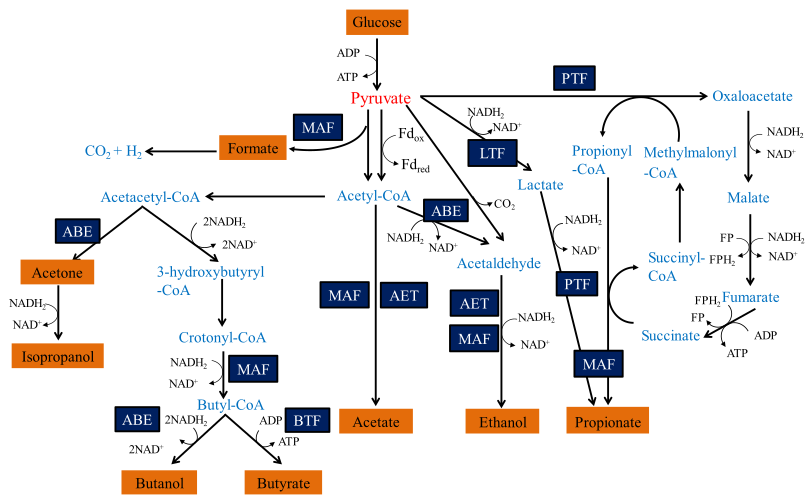
\includegraphics[width=.9\linewidth]{../plots/metabolic_results/pyruvate_metabolism_zhou.png}
\caption[Μεταβολικά μονοπάτια κατανάλωσης του πυροσταφυλικού οξέος]{\label{fig:orgafbdbba}Μεταβολικά μονοπάτια κατανάλωσης του πυροσταφυλικού οξέος \textsuperscript{\citeprocitem{70}{70}}}
\end{figure}

Στο σύστημα μετά την οξείδωση της γλυκόζης επικρατούν αναγωγικές συνθήκες. Οπότε, είναι πολύ πιθανό να διεξαχθούν αναγωγικές αντιδράσεις. Η απλούστερη αναγωγική αντίδραση είναι η αναγωγή του πυροσταφυλικού οξέος σε γαλακτικό οξύ. Σε πολλές περιπτώσεις, το γαλακτικό οξύ μπορεί να αναχθεί περαιτέρω σε προπιονικό οξύ μέσω του \acrshort{nadh}. Γενικά, το γαλακτικό οξύ επικρατεί σε όξινα pH (4.0-5.0) ενώ με την αύξηση του pH παράγεται περισσότερο προπιονικό. Βέβαια, ακόμη και στα pH που το γαλακτικό επικρατεί, λόγω του υψηλού αναγωγικού φορτίου που είναι διαθέσιμο, θα παραχθεί κάποια ποσότητα προπιονικού. Το μονοπάτι αυτό λέγεται ομογαλακτική ζύμωση, επειδή παράγονται 2 mol γαλακτικού ανά mol γλυκόζης, σε αντίθεση με την ετερογαλακτική ζύμωση όπου παράγεται 1 mol γαλακτικού ανά mol γλυκόζης \textsuperscript{\citeprocitem{70}{70},\citeprocitem{71}{71}} .

Το προπιονικό μπορεί να παραχθεί και από άλλο ένα μονοπάτι, το transcarboxylase cycle, το οποίο είναι ένα κυκλικό μονοπάτι μεταξύ οργανικών οξέων με 4 άνθρακες, το οποίο ξεκινάει λόγω της εναλλαγής ενός CO\textsubscript{2} μεταξύ του πυροσταφυλικού οξέος και του μεθυλομηλονικού οξέος, το οποίο μετατρέπεται σε προπιονικό οξύ λόγω αυτού. Ως μεταβολικό προϊόν, μπορεί να παραχθεί σε μεγάλο εύρος pH, αλλά δεν είναι πουθενά το κύριο προϊόν καθώς οι μικροοργανισμοί που παράγουν προπιονικό οξύ αναστέλλονται ισχυρά από το προπιονικό οξύ \textsuperscript{\citeprocitem{70}{70}} . Γενικά, είναι σπάνιο να συσσωρευθεί οποιοδήποτε από τα ενδιάμεσα του κύκλου αυτού, αλλά με το κατάλληλο μικροβιακό πληθυσμό, σε ουδέτερο προς αλκαλικό pH (7-8.5) και συσσώρευση CO\textsubscript{2}, μπορεί να παρατηρηθεί συσσώρευση ηλεκτρικού οξέος στον αντιδραστήρα \textsuperscript{\citeprocitem{64}{64}} . Ο λόγος που αν συσσωρευτεί κάτι, θα είναι το ηλεκτρικό οξύ, είναι επειδή αυτό αποτελεί το στάδιο του κύκλου το οποίο περιορίζει τον ρυθμό, οπότε αν διακοπεί κάπου ενδιάμεσα, θα είναι στο στάδιο αυτό \textsuperscript{\citeprocitem{72}{72}} .

Η άλλη βασική αντίδραση κατανάλωσης του πυροσταφυλικού, είναι η οξείδωση του σε \acrshort{acet-coa}. Αυτή δεν καταλύεται από το \acrshort{nad} καθώς στις αναγωγικές συνθήκες που επικρατούν αυτό βρίσκεται στην μορφή του \acrshort{nadh}, αλλά από ένα είδος πρωτεϊνών γνωστές ως \acrfull{fd}. Οι πρωτεΐνες αυτές αποτελούνται από σίδηρο και χαλκό και συνεισφέρουν σε καταλυτικές αντιδράσεις, ανάλογα με την οξειδωτική κατάσταση του σιδήρου. Είναι πιο ισχυρό οξειδοαναγωγικό μέσο από το \acrshort{nad}, οπότε μπορεί να καταλύσει την αντίδραση αυτή παρότι το περιβάλλον είναι αρκετά αναγωγικό \textsuperscript{\citeprocitem{65}{65},\citeprocitem{70}{70},\citeprocitem{73}{73}} . Η αντίδραση αυτή παράγει και ένα mol CO\textsubscript{2} και H\textsubscript{2} κατά την οξείδωση. Οι δύο ενώσεις αυτές βρίσκονται σε ισορροπία με το μυρμηκικό οξύ \(H_2 + CO_2 \rightleftharpoons HCOOH\). Η αντίδραση αυτή έχει \acrfull{dg} αρκετά κοντά στο 0, οπότε, το αν τα δύο αέρια θα είναι σε ελεύθερη μορφή ή θα μετατραπούν σε μυρμηκικό οξύ εξαρτάται σε μεγάλο βαθμό από τις συνθήκες. Η βασικότερη εξάρτηση είναι το pH. Το μυρμηκικό οξύ παρατηρείται γενικά σε pH από 7 και πάνω, ενώ σε χαμηλότερες τιμές η μετατροπή είναι θερμοδυναμικά ανέφικτη. Ο ρόλος του μυρμηκικού οξέος στο σύστημα είναι ότι είναι ένα εναλλακτικό αναγωγικό μέσο, όταν το υδρογόνο δεν είναι στην ελεύθερη μορφή. Δεν συμμετέχει σε άλλες μεταβολικές αντιδράσεις οξεογένεσης \textsuperscript{\citeprocitem{64}{64}} .

Από το \acrshort{acet-coa} παράγονται τα υπόλοιπα προϊόντα της διεργασίας. Το πιο "εύκολο" μεταβολικό προϊόν είναι το οξικό οξύ. Παράγεται απευθείας από το \acrshort{acet-coa} ανεξάρτητα από το \acrfull{redox} και σε μεγάλο εύρος pH. Οπότε, είναι το κύριο προϊόν του \acrshort{acet-coa} εκτός αν λόγω συνθηκών επικρατήσει κάποιο άλλο \textsuperscript{\citeprocitem{61}{61},\citeprocitem{74}{74}} . Επίσης, οξικό οξύ παράγεται ως συμπροϊόν των αναγωγικών προϊόντων (γαλακτικό και προπιονικό) για να εξισορροπήσει το \acrshort{orp}.

Τα άλλα βασικά προϊόντα από το \acrshort{acet-coa} είναι η αιθανόλη και το βουτυρικό οξύ. Η αιθανόλη παράγεται από την αναγωγή του \acrshort{acet-coa} με ενδιάμεσο την φορμαλδεΰδη. Μεγάλες ποσότητες αιθανόλης παρατηρούνται σε πολύ όξινα pH (4.0-4.5) και ξανά εμφανίζονται σε αλκαλικά pH (8.0) \textsuperscript{\citeprocitem{62}{62},\citeprocitem{64}{64},\citeprocitem{75}{75}} . Η ισορροπία αιθανόλης/οξικού είναι μία αρκετά ενδιαφέρουσα ισορροπία. Η αιθανόλη παράγεται από το \acrshort{acet-coa} οπότε η παραγωγή οξικού οξέος ως συμπροϊόν της δεν γίνεται για εξισορρόπηση του \acrshort{orp}. Όμως, συνήθως δεν υπάρχει αρκετό αναγωγικό δυναμικό για να παραχθεί μόνο αιθανόλη. Το πιο συχνά παρατηρούμενο είναι 1 mol γλυκόζης να μετατραπεί σε ένα ισομοριακό μείγμα αιθανόλης και οξικού οξέος, επειδή όλο το αναγωγικό δυναμικό χρησιμοποιείται για την παραγωγή ενός mol αιθανόλης και άρα το άλλο \acrshort{acet-coa} μετατρέπεται σε οξικό. Το μονοπάτι αυτό ονομάζεται ζύμωση αιθανόλης-οξικού \textsuperscript{\citeprocitem{70}{70},\citeprocitem{74}{74},\citeprocitem{75}{75}} . 

Το βουτυρικό οξύ παράγεται από το acetacetyl-CoA, το οποίο είναι το προϊόν της αντίδρασης 2 mol \acrshort{acet-coa}. Μετά από δύο αναγωγές, αυτό μετατρέπεται σε butyryl-CoA, το οποίο μετατρέπεται αυθόρμητα σε βουτυρικό οξύ. Έτσι, το βουτυρικό οξύ είναι το μόνο από τα κύρια προϊόντα του μεταβολισμού του πυροσταφυλικού οξέος το οποίο απαιτεί 2 mol πυροσταφυλικού για να παραχθεί. Αποτελεί το κύριο συμπροϊόν του οξικού οξέος σε pH από 5 εώς 6.5. Παράγεται ως συμπροϊόν του οξικού επειδή όπως και για την αιθανόλη, συχνά δεν φτάνει το αναγωγικό δυναμικό για να παραχθεί μόνο του και κάποια mol \acrshort{acet-coa} θα μετατραπούν σε οξικό \textsuperscript{\citeprocitem{61}{61},\citeprocitem{62}{62},\citeprocitem{70}{70}} .

Στην περίπτωση που το pH ξεπεράσει το 6.5, σταματάει να επικρατεί κάποιο οξεογενετικό προϊόν και προτιμάται το μονοπάτι γνωστό ως ζύμωση μικτών οξέων, όπου παράγονται: μυρμηκικό, οξικό, προπιονικό, βουτυρικό και βαλερικό οξύ σε κάποια περιεκτικότητα. Αυτό είναι το μεταβολικό μονοπάτι που ακολουθείται και στην περίπτωση που η οξεογένεση διεξάγεται ταυτόχρονα με την μεθανογένεση, καθώς αυτό είναι το pH στο οποίο διεξάγεται η μεθανογένεση. Αυτό το μονοπάτι δεν είναι ιδιαίτερα επιθυμητό στην περίπτωση που ελέγχεται η οξεογένεση, επειδή προτιμάται ένα πιο ελεγχόμενο προφίλ προϊόντων \textsuperscript{\citeprocitem{61}{61},\citeprocitem{64}{64},\citeprocitem{70}{70}} .

Ένα τελευταίο μονοπάτι, το οποίο αξίζει να σημειωθεί, παρόλο που δεν παρατηρείται σε μία τυπική οξεογενή ζύμωση είναι η \acrfull{abe}. Η αιθανόλη έχει ήδη αναφερθεί ως προϊόν της οξεογενετικής ζύμωσης. Όπως φαίνεται στο \figurename \ref{fig:orgafbdbba}, η βουτανόλη παράγεται από την αναγωγή του butyryl-CoA σε ισορροπία με το βουτυρικό οξύ, αντίστοιχη με αυτήν του οξικού με την αιθανόλη. Η ακετόνη, είναι εναλλακτικό προϊόν του Acetacetyl-CoA. Ο μηχανισμός της ζύμωσης αυτής είναι πως ξεκινάει με οξεογένεση και συγκεκριμένα ζύμωση οξικού-βουτυρικού, καθώς διεξάγεται συνήθως σε pH 5.5-6.0, όπου επικρατούν τα δύο αυτά προϊόντα, και σταδιακά μετατρέπεται σε διαλυτογένεση (solventogenesis), όπου το acetyl-CoA παράγει αιθανόλη ενώ το acetacetyl-CoA παράγει ακετόνη και βουτανόλη. Βέβαια, για να γίνει αυτό απαιτούνται κάποια ειδικά βακτήρια τα οποία έχουν το μονοπάτι της διαλυτογένεσης. Αυτά είναι μία κατηγορία των βακτηρίων του γένους Clostridium \textsuperscript{\citeprocitem{47}{47},\citeprocitem{70}{70}} .

\section{Αλλα μονοπάτια μεταβολισμού της γλυκόζης}
\label{sec:org34fdd97}
Το μονοπάτι \acrshort{emp} το οποίο έχει αναλυθεί έως τώρα είναι το πιο συχνό μονοπάτι μεταβολισμού της γλυκόζης. Όμως, δεν είναι το μοναδικό μονοπάτι στο οποίο μπορεί να μεταβολιστεί η γλυκόζη. Στο σχήμα \figurename \ref{fig:orgdd687f5} φαίνονται όλα τα μεταβολικά μονοπάτια μεταβολισμού της γλυκόζης \textsuperscript{\citeprocitem{62}{62}} .

\begin{figure}[htbp]
\centering
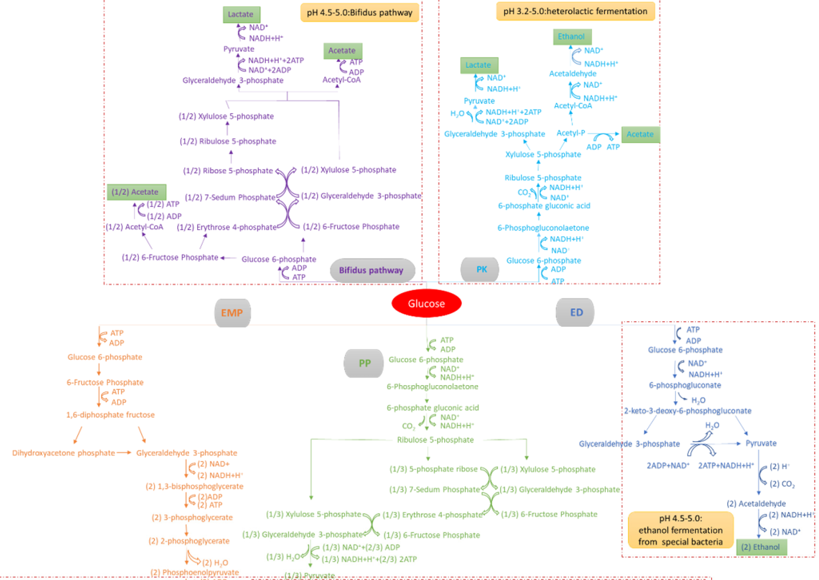
\includegraphics[width=.9\linewidth]{../plots/metabolic_results/glucose_metabolism_qiao.png}
\caption[Μεταβολικά Μονοπάτια της Γλυκόζης]{\label{fig:orgdd687f5}Μεταβολικά Μονοπάτια της Γλυκόζης \textsuperscript{\citeprocitem{61}{61}}}
\end{figure}

Το \acrfull{ed} είναι το μονοπάτι παραγωγής 2 mol αιθανόλης από ένα mol γλυκόζης και υπάρχει κυρίως σε ζύμες. Παρατηρείται σπανίως σε μικτές καλλιέργειες βακτηρίων όπως αυτές που χρησιμοποιούνται στην \acrshort{ad} δύο σταδίων. Το \acrfull{pp} είναι ένα μονοπάτι παρόμοιο του \acrshort{emp} καθώς κάθε mol γλυκόζη μετατρέπεται σε 1/3 mol πυροσταφυλικό και 2/3 mol fructose 6-P το οποίο μπορεί να μεταβολιστεί σε πυροσταφυλικό \textsuperscript{\citeprocitem{61}{61},\citeprocitem{62}{62}} .

Τα άλλα 2 μονοπάτια που παρουσιάζονται στο \figurename  \ref{fig:orgdd687f5} είναι και τα σημαντικότερα. Το \acrfull{pk}, γνωστό και ως ετερογαλακτική ζύμωση είναι ένα μονοπάτι στο οποίο παράγονται ως τελικά προϊόντα ένα μείγμα γαλακτικού οξέος και αιθανόλης, ή σπανίως οξικού οξέος. Στο μονοπάτι αυτό, παράγεται η ένωση Xylulose 5-Phosphate μετά από 2 οξειδώσεις με αποτέλεσμα να υπάρχει περίσσεια αναγωγικού φορτίου. Η ένωση αυτή διασπάται σε Glyceraldehyde 3-Phosphate - ένωση από την οποία μπορεί να παραχθεί πυροσταφυλικό - και \acrshort{acet-coa}. Καθώς υπάρχει πολύ αναγωγικό δυναμικό στο μονοπάτι αυτό, είναι αρκετά σπάνιο να παραχθεί οξικό οξύ, οπότε παράγεται γαλακτικό οξύ από το πυροσταφυλικό και αιθανόλη από το \acrshort{acet-coa}. Αυτό το μονοπάτι έχει την ιδιαιτερότητα ότι λειτουργεί συνήθως σε pH 4.0-5.0, αλλά μπορεί να γίνει και σε pH κάτω από 4.0 ιδιαίτερα αποτελεσματικά \textsuperscript{\citeprocitem{61}{61},\citeprocitem{62}{62}} . Από άποψη μικροβιακής ποικιλότητας, αυτό το μονοπάτι γίνεται από διάφορα βακτήρια, κυρίως του γένους Lactobacillus, τα οποία είναι ιδιαίτερα ενεργά σε \acrshort{fw}. Για αυτό είναι ιδιαίτερα συχνό μονοπάτι όταν χρησιμοποιείται αυτό το υπόστρωμα \textsuperscript{\citeprocitem{71}{71},\citeprocitem{76}{76}} .

Το μονοπάτι Bifidus είναι παρόμοιο του \acrshort{pk}, καθώς και σε αυτό παράγεται 1 mol Xylulose-5-phosphate. Η βασική διαφορά είναι το πως φτάνει στην ένωση αυτή. Δεν υπάρχει κανένα οξειδωτικό βήμα, με αποτέλεσμα το αναγωγικό δυναμικό στην περίπτωση αυτή να είναι πολύ χαμηλό. Οπότε, το Acetyl-CoA θα μετατραπεί σε οξικό, ενώ το πυροσταφυλικό θα μετατραπεί σε γαλακτικό λόγω του σταδίου οξείδωσης του glyceraldehyde 3-phosphate σε πυροσταφυλικό, το οποίο δημιουργεί αναγωγικό δυναμικό που πρέπει να αξιοποιηθεί. Μία ακόμη διαφορά του μονοπατιού αυτού είναι πως ο ένας άνθρακας που αποβάλλεται για να δημιουργηθεί το Xylulose-5-phosphate δεν γίνεται CO\textsubscript{2}, αλλά μισό mol \acrshort{acet-coa}, το οποίο μετατρέπεται και αυτό σε οξικό, με αποτέλεσμα κάθε mol γλυκόζης να δίνει 1.5 mol οξικό και 1 mol γαλακτικό. Το μονοπάτι αυτό γίνεται σε λίγο πιο υψηλά pH από το \acrshort{pk} όπως 4.5-5.5 \textsuperscript{\citeprocitem{61}{61},\citeprocitem{71}{71}} . 

\section{Απόκριση της οξεογένεσης}
\label{sec:orgf433ca6}
Έχοντας εξετάσει όλα τα δυνατά μονοπάτια της οξεογενετικής ζύμωσης, φτάνει τώρα να εισαχθούν κάποια ποσοτικά στοιχεία για το πως κρίνεται η ποιότητα της οξεογένεσης. Ένα βασικό κριτήριο είναι προφανώς το προφίλ των προϊόντων \textsuperscript{\citeprocitem{76}{76},\citeprocitem{77}{77}}. Άλλωστε, αν δεν είχε σημασία το προφίλ αυτό, δεν θα υπήρχε ενδιαφέρον στον έλεγχο του μονοπατιού της οξεογένεσης. Η ποιότητα όμως του κάθε προϊόντος για την αναερόβια χώνευση θα αναλυθεί στο \autoref{sec:methanogenesis}.

Ένα άλλο, πιο γενικό κριτήριο για να κριθεί η οξεογένεση είναι τα \acrfull{tvfa}. Συγκεκριμένα, αν αυτά εκφραστούν στο ισοδύναμο \acrshort{cod} τους, μπορούν να συγκριθούν με το \acrshort{scod}. Σε μία καλή οξεογένεση, ο λόγος \acrfull{tvfa} προς \acrshort{scod}, ο οποίος είναι γνωστός ως οξίνιση του αντιδραστήρα είναι \(80-90 \%\) \textsuperscript{\citeprocitem{45}{45},\citeprocitem{77}{77}} .

\chapter{Οξικογένεση και Μεθανογένεση}
\label{sec:org1a000a5}
\label{sec:methanogenesis}

Στα προηγούμενα κεφάλαια αναλύθηκαν εις βάθος η υδρόλυση και η οξεογένεση, τα 2 πρώτα στάδια της \acrshort{ad}, τα οποία είναι και αυτά που συνήθως διαχωρίζονται όταν η διεργασία διεξάγεται σε 2 στάδια. Συγκεκριμένα, στο \autoref{sec:acidogenesis} αναλύθηκαν όλα τα πιθανά μονοπάτια οξεογένεσης και τα προϊόντα του καθενός, και αναφέρθηκε πως είναι επιθυμητό να ελεγχθεί το μεταβολικό μονοπάτι που θα ακολουθηθεί, επειδή δεν είναι όλα τα προϊόντα το ίδιο χρήσιμα για την μεθανογένεση. Για να επεξηγηθεί αυτό, θα πρέπει να εξεταστεί σε βάθος ο μηχανισμός με τον οποίο διεξάγεται η μεθανογένεση, το οποίο είναι ο σκοπός του κεφαλαίου αυτού.
\section{Μηχανισμός Μεθανογένεσης}
\label{sec:org090619b}
Η μεθανογένεση είναι το σημαντικότερο αλλά και πιο ευαίσθητο στάδιο της αναερόβιας χώνευσης. Γίνεται από μικροοργανισμούς του κλάδου των αρχαίων, οι οποίοι είναι υποχρεωτικά αναερόβιοι μικροοργανισμοί με στενό λειτουργικό εύρος pH (περίπου 6.4-8.0). Τα αρχαία τα οποία παράγουν μεθάνιο διαχωρίζονται σε δύο βασικές κατηγορίες, τους ακετοκλαστικούς μεθανογόνους (\acrshort{am}), οι οποίοι χρησιμοποιούν το οξικό οξύ ως υπόστρωμα και τους υδρογονοτρόφους μεθανογόνους (\acrshort{hm}), οι οποίοι ανάγουν διοξείδιο του άνθρακα σε μεθάνιο παρουσία υδρογόνου. Σε κανονικές συνθήκες, περίπου 2/3 του μεθανίου παράγονται από τους \acrshort{am} ενώ τα υπόλοιπα από τους \acrshort{hm} \textsuperscript{\citeprocitem{72}{72},\citeprocitem{78}{78}} .

Για να έχουν υπόστρωμα οι μικροοργανισμοί αυτοί, πρέπει όλα τα προϊόντα της οξεογένεσης να μετατραπούν σε οξικό οξύ και υδρογόνο. Για αυτό υπάρχει το στάδιο της οξικογένεσης. Στο στάδιο αυτό, τα διάφορα προϊόντα που παράχθηκαν κατά την οξεογένεση μετατρέπονται σε οξικό οξύ, ενώ ταυτόχρονα παράγεται και υδρογόνο, καθώς όλες οι αντιδράσεις αυτές είναι οξειδωτικές. Σε αντίθεση όμως με τα 2 προηγούμενα και το επόμενο στάδιο, τα οποία γίνονται αυθόρμητα αν υπάρχει το κατάλληλο μικροβιακό δυναμικό, υπόστρωμα και λειτουργικές συνθήκες, οι περισσότερες οξικογενετικές αντιδράσεις δεν είναι αυθόρμητες σε καμία περιοχή του λειτουργικού εύρους που εξετάζεται \textsuperscript{\citeprocitem{79}{79}} . Ο μηχανισμός με τον οποίο διεξάγονται οι αντιδράσεις αυτές είναι γνωστός ως συντροφικός μεταβολισμός. Για κάθε ένα από τα συχνά προϊόντα της οξεογένεσης, το άθροισμα των αντιδράσεων οξικογένεσης και παραγωγής μεθανίου από οξικό οξύ και υδρογόνο έχει αρνητική \acrshort{dg}, δηλαδή είναι αυθόρμητο. Οπότε, μπορεί να γίνει η αντίδραση οξικογένεσης, η οποία δεν είναι επιθυμητή για το σύστημα, επειδή τα προϊόντα της θα μεταβολιστούν από τους μεθανογόνους και ο συνδυασμός θα είναι ενεργειακά ωφέλιμος \textsuperscript{\citeprocitem{78}{78}–\citeprocitem{80}{80}} .

Με βάση αυτό, ένα από τα βασικά κριτήρια για την ποιότητα ενός προϊόντος για αναερόβια χώνευση, είναι η θερμοδυναμική των αντιδράσεων αυτών, η οποία θα αναλυθεί παρακάτω.

\section{Θερμοδυναμική Παραγωγής Μεθανίου}
\label{sec:org487d1f1}
\label{sec:methane-thermodynamics}

Τα προϊόντα τα οποία θα συζητηθούν εδώ θα είναι τα εξής: Οξικό οξύ, προπιονικό οξύ, γαλακτικό οξύ, βουτυρικό οξύ, αιθανόλη. Τα υπόλοιπα προϊόντα που μπορούν να παραχθούν από οξεογένεση ή δεν παράγονται σε μεγάλη ποσότητα (πχ βαλερικό οξύ), ή όταν παράγονται, ο σκοπός της διεργασίας δεν είναι η παραγωγή μεθανίου (πχ ακετόνη ή βουτανόλη) \textsuperscript{\citeprocitem{47}{47},\citeprocitem{79}{79},\citeprocitem{81}{81}} . Ως αρχικό υπόστρωμα θα εξεταστεί η γλυκόζη, καθώς τα σάκχαρα είναι και το συχνότερο υπόστρωμα της \acrshort{ad}, ενώ αντίστοιχα λειτουργεί και ο μεταβολισμός άλλων υποστρωμάτων.

Η μετατροπή της γλυκόζης σε μεθάνιο (\(C_6H_{12}O_6 \rightarrow 3CH_4 + 3CO_2\)) είναι μία αυθόρμητη αντίδραση με \acrshort{dg} = - 404 kJ/mol σε πρότυπες συνθήκες \textsuperscript{\citeprocitem{79}{79}} . Από τον νόμο του Hess, είναι γνωστό πως η ενθαλπία (και κατ'επέκτασιν η ελεύθερη ενέργεια Gibbs) μίας αντίδρασης είναι ίδια ανεξαρτήτως του μονοπατιού με το οποίο έγινε η αντίδραση. Οπότε, ανεξαρτήτως του ενδιαμέσου, το σύστημα της \acrshort{ad} θα παράγει αυτή την ενέργεια για αυτήν την μετατροπή. Όμως, όσο πιο κοντά στο 0 είναι το άθροισμα των \acrshort{dg} της οξικογένεσης και μεθανογένεσης, τόσο πιο δύσκολο είναι να ολοκληρωθεί η αντίδραση με βάση το μονοπάτι αυτό, με αποτέλεσμα η \acrshort{ad} να μην λειτουργεί σωστά. Ακόμη, οι \acrshort{dg} που θα αναφερθούν παρακάτω είναι σε πρότυπες συνθήκες. Σε διαφορετικά pH (δηλαδή συγκέντρωση υδρογονοκατιόντων) ή σε διαφορετική συγκέντρωση του κάθε προϊόντος, μπορεί η \acrshort{dg} της αντίδρασης να είναι διαφορετική. Οπότε, αν είναι κοντά στο 0 σε πρότυπες συνθήκες, είναι πιθανόν να υπάρχει συνθήκη όπου η αντίδραση δεν μπορεί πλέον να συνεχίσει.

\begin{enumerate}
\item Οξικό Οξύ:
\label{sec:org5275b60}
Το οξικό οξύ είναι το ιδανικό υπόστρωμα για μεθανογένεση καθώς είναι το μόνο που μεταβολίζεται απευθείας σε μεθάνιο. Οι αντιδράσεις μεθανογένεσης που διεξάγονται είναι οι

\begin{subequations}
\label{eqn:methanogenesis}
\begin{align}
2CH_3COO^- + 2H_2O &\rightarrow 2CH_4 + 2HCO_3^- & \text{ΔG = - 62.0 kJ} \label{eqn:acet-methane} \\
4H_2 + HCO_3^- + H^+ &\rightarrow CH_4 + 3H_2O & \text{ΔG = -135.6 kJ} \label{eqn:hydro-methane} \\
\hline
2CH_3COO^- + 4H_2 + H^+ &\rightarrow 3 CH_4 + HCO_3^- + H_2O & \text{ΔG = -197.6 kJ} \label{eqn:complete-methane}
\end{align}
\end{subequations}

με αποτέλεσμα το στάδιο αυτό να είναι αυθόρμητο με \acrshort{dg} = -197.6 kJ, δηλαδή σχεδόν η μισή ενέργεια που παράγεται κατά την μετατροπή της γλυκόζης σε μεθάνιο να οφείλεται στην μεθανογένεση (αξίζει να αναφερθεί πως οι συντελεστές είναι με βάση τις ποσότητες που παράγει 1 mol γλυκόζη) \textsuperscript{\citeprocitem{79}{79}} .

\item Προπιονικό Οξύ:
\label{sec:orgf40a9f1}
Το προπιονικό οξύ είναι συχνό αναγωγικό προϊόν του μεταβολισμού του πυροσταφυλικού οξέος και παρατηρείται συχνά στην \acrshort{ad} \textsuperscript{\citeprocitem{70}{70},\citeprocitem{74}{74}} . Εκτός από τις αντιδράσεις \ref{eqn:acet-methane}, \ref{eqn:hydro-methane}, γίνεται και η αντίδραση

\begin{align}
2CH_3CH_2COO^- + 6H_2O &\rightarrow 2CH_3COO^- + 2HCO_3^- + 2H^+ + 6H_2 & \text{ΔG = + 152.2 kJ}
\label{eqn:prop-acet}
\end{align}

με αποτέλεσμα, το άθροισμα οξεογένεσης και μεθανογένεσης να είναι -45.4 kJ και μόνο ένα \(11.4 \%\) της συνολικής ενέργειας να οφείλεται στην μεθανογένεση. Η αντίδραση αυτή παραμένει αυθόρμητη, όμως αποτελεί μία πολύ πιο δύσκολη αντίδραση, διότι οι μεθανογόνοι σπαταλούν πολύ περισσότερη ενέργεια για να διεξαχθεί \textsuperscript{\citeprocitem{72}{72},\citeprocitem{79}{79}}. Επιπλέον, σε συνθήκες μακριά από τις πρότυπες (πχ μεγάλη μερική πίεση υδρογόνου ή πολύ όξινο περιβάλλον), η \acrshort{dg} την αντίδρασης \ref{eqn:prop-acet} θα είναι ακόμη μεγαλύτερη, με αποτέλεσμα το άθροισμα να είναι ακόμη πιο κοντά στο 0. Σε ακραίες περιπτώσεις, έχει παρατηρηθεί και κατάρρευση του συστήματος της \acrshort{ad} επειδή έχει παραχθεί πολύ προπιονικό οξύ και στις συνθήκες που υπάρχουν, δεν μπορεί να μετατραπεί σε μεθάνιο. Οπότε, το προπιονικό οξύ είναι γενικά ένα αρκετά ανεπιθύμητο προϊόν \textsuperscript{\citeprocitem{79}{79},\citeprocitem{82}{82},\citeprocitem{83}{83}} . Όμως, καθώς αποτελεί το βασικότερο αναγωγικό προϊόν της οξεογένεσης, συχνά δεν μπορεί να αποφευχθεί πλήρως \textsuperscript{\citeprocitem{70}{70}}. Στην βιβλιογραφία, έχουν προταθεί τρόποι για να γίνει πιο εύκολη η αντίδραση αυτή και να μην αναστέλλει το σύστημα, όπως η προσθήκη σιδήρου μηδενικού σθένους (\acrshort{zvi}), ο οποίος μειώνει αρκετά το \acrshort{redox} του αντιδραστήρα, το οποίο κάνει πολύ πιο αρνητικό το \acrshort{dg} της αντίδρασης \textsuperscript{\citeprocitem{84}{84}} αλλά και άλλες τεχνολογίες όπως η προσθήκη κάποιου buffer, ή απαραίτητων ιχνοστοιχείων για να γίνει πιο αποτελεσματική η αντίδραση \textsuperscript{\citeprocitem{72}{72}} .

\item Γαλακτικό Οξύ:
\label{sec:org43c08f3}
Το άλλο συχνό αναγωγικό προϊόν είναι το γαλακτικό οξύ, το οποίο όπως αναφέρθηκε, παράγεται σε μεγάλες ποσότητες κατά την ζύμωση \acrshort{fw} \textsuperscript{\citeprocitem{71}{71},\citeprocitem{76}{76}} . Το γαλακτικό οξύ είναι ένα ενδιαφέρον ενδιάμεσο για την \acrshort{ad} καθώς η αναγωγή του σε προπιονικό οξύ και η οξείδωση του σε οξικό είναι και οι δύο κοντά στην ισορροπία. Σε πρότυπες συνθήκες είναι οι εξής: \textsuperscript{\citeprocitem{79}{79},\citeprocitem{85}{85}}

\begin{subequations}
\label{eqn:lact-redox}
\begin{align}
2CH_3CHOHCOO^- &\rightarrow 2CH_3COO^- + 2HCO_3^- + 2H^+ + 4H_2 & \text{ΔG = - 8.4 kJ} \label{eqn:lact-ox} \\
2CH_3CHOHCOO^- &\xrightarrow{2NADH \rightarrow 2NAD^+} 2CH_3CH_2COO^- & \text{ΔG = 27.6 kJ} \label{eqn:lact-red}
\end{align}
\end{subequations}

Επίσης υπενθυμίζεται πως το ζεύγος \acrshort{nadh} με \acrshort{nad} είναι ένα οξειδωαναγωγικό ζεύγος με την ισορροπία

\begin{align}
NADH + H^+ &\rightleftharpoons NAD^+ + H_2 & ΔG = - 21.8 \frac{kJ}{mol}
\label{eqn:nadh}
\end{align}

Άρα, σε πρότυπες συνθήκες, θερμοδυναμικά επιθυμητή είναι η αντίδραση \ref{eqn:lact-ox}, οπότε θεωρητικά θα έπρεπε το γαλακτικό οξύ να είναι ένα ιδιαίτερα επιθυμητό προϊόν της \acrshort{ad}. Όμως, η \acrshort{ad} λειτουργεί σε ένα αρκετά αναγωγικό περιβάλλον, όπου το \acrshort{nadh} είναι συχνότερα στην ανηγμένη μορφή του και άρα η \ref{eqn:lact-red} ευνοείται πολύ περισσότερο, ενώ η \ref{eqn:lact-ox} έχει γίνει θερμοδυναμικά ανέφικτη. Βέβαια, η συντροφική δράση των μικροοργανισμών αυτών με τους μεθανογόνους κάνει την αντίδραση αυτή εφικτή, όπως και για τα άλλα προϊόντα. Στην πράξη, o πιο συχνός μεταβολισμός του γαλακτικού οξέος είναι ένας μικτός μεταβολισμός με βάση την αντίδραση

\begin{align}
3CH_3CHOHCOOH &\rightarrow 2CH_3CH_2COOH + CH_3COOH + HCO_3^- + H^+ & \text{ΔG = -165 kJ}
\label{eqn:mixed-lact}
\end{align}

Η αντίδραση αυτή είναι μία οξειδωαναγωγική αντίδραση όπου τα υδρογόνα της \ref{eqn:lact-ox} χρησιμοποιούνται για την \ref{eqn:lact-red} με αποτέλεσμα μία ιδιαίτερα θερμοδυναμική επιθυμητή αντίδραση. Αυτή είναι η αντίδραση που ακολουθείται όταν και οι δύο αντιδράσεις είναι πολύ κοντά σε ισορροπία \textsuperscript{\citeprocitem{85}{85}} . 

Οπότε, το γαλακτικό οξύ δεν είναι ένα ιδιαίτερα επιθυμητό ενδιάμεσο, λόγω της πιθανότητας να μεταβολιστεί σε προπιονικό \textsuperscript{\citeprocitem{79}{79}}, αλλά υπό τις κατάλληλες συνθήκες αποτελεί ένα πολύ καλό ενδιάμεσο της διεργασίας και κάποιες μελέτες έχουν δείξει πολύ καλή απόδοση στην \acrshort{ad} από υπόστρωμα πλούσιο σε γαλακτικό \textsuperscript{\citeprocitem{76}{76},\citeprocitem{84}{84}} .

\item Βουτυρικό Οξύ:
\label{sec:orgfd7dd0b}
Το βουτυρικό οξύ είναι ένα ακόμη σύνηθες προϊόν της οξεογένεσης \textsuperscript{\citeprocitem{70}{70},\citeprocitem{77}{77}} . Η οξικογένεση του βουτυρικού είναι η αντίδραση

\begin{align}
CH_3CH_2CH_2COO^- + 2H_2O &\rightarrow 2CH_3COO^- + H^+ + 2H_2 & \text{ΔG = + 48.1 kJ}
\label{eqn:but-ox}
\end{align}

Η αντίδραση αυτή δεν είναι αυθόρμητη σε πρότυπες συνθήκες, αλλά σε συντροφικό μεταβολισμό με τις αντιδράσεις \ref{eqn:methanogenesis} έχει ένα τελικό \acrshort{dg} = -149.5 kJ \textsuperscript{\citeprocitem{79}{79},\citeprocitem{85}{85}}. Γενικά το βουτυρικό οξύ είναι ένα προϊόν το οποίο μετατρέπεται εύκολα σε μεθάνιο λόγω αυτού και υπάρχουν μελέτες που έχουν δείξει πως είναι ένα από τα πιο επιθυμητά προϊόντα της οξεογένεσης \textsuperscript{\citeprocitem{70}{70},\citeprocitem{77}{77},\citeprocitem{83}{83}} .

\item Αιθανόλη:
\label{sec:org97c3293}
Η αιθανόλη είναι το τελευταίο προϊόν το οποίο θα εξεταστεί. Αποτελεί ένα αναγωγικό προϊόν του \acrshort{acet-coa} που παράγεται ως συμπροϊόν του οξικού οξέος σε χαμηλά pH \textsuperscript{\citeprocitem{61}{61},\citeprocitem{70}{70}} . Η αιθανόλη μπορεί να μετατραπεί σε οξικό αρκετά εύκολα για τον λόγο αυτό. Η αντίστοιχη αντίδραση είναι η

\begin{align}
2C_2H_5OH + 2H_2O &\rightarrow 2CH_3COO^- + 2H^+ + 4H_2 & \text{ΔG = + 19.2 kJ}
\label{eqn:eth-acet}
\end{align}

η οποία έχει θετική αλλά χαμηλή \acrshort{dg} με αποτέλεσμα σε συνδυασμό με τις αντιδράσεις \ref{eqn:methanogenesis} να έχει \acrshort{dg} = -178.4 kJ, το οποίο καθιστά την μετατροπή της αιθανόλης σε μεθάνιο αρκετά εύκολη. Ακόμη, σε ορισμένες συνθήκες (χαμηλή μερική πίεση υδρογόνου, υψηλή συγκέντρωση αιθανόλης) μπορεί η αντίδραση αυτή να γίνει αυθόρμητη και από μόνη της και να παρατηρηθεί οξικογένεση χωρίς συντροφική μεθανογένεση \textsuperscript{\citeprocitem{79}{79},\citeprocitem{85}{85}} . 

Εκτός από το γεγονός ότι είναι ένα ενδιάμεσο που μετατρέπεται εύκολα σε μεθάνιο και άρα είναι καλό για μεθανογένεση \textsuperscript{\citeprocitem{76}{76},\citeprocitem{86}{86}}, η αιθανόλη έχει δείξει να βελτιώνει την ρυθμιστική ικανότητα του αντιδραστήρα \textsuperscript{\citeprocitem{87}{87}} και να προάγει το μεταβολικό μονοπάτι \acrfull{diet} για την μεθανογένεση, το οποίο είναι πολύ ενεργειακά αποτελεσματικό \textsuperscript{\citeprocitem{88}{88}–\citeprocitem{90}{90}} . Τα πλεονεκτήματα του μονοπατιού αυτού έναντι του συμβατικού (\acrfull{iht}) θα αναλυθούν περισσότερο παρακάτω.
\end{enumerate}

\section{Πλεονεκτήματα του Direct Interspecies Electron Transfer στην Mεθανογένεση}
\label{sec:org7216e41}
Το συμβατικό μοντέλο συντροφικού μεταβολισμού μεταξύ των οξικογόνων μικροοργανισμών και των μεθανογόνων, βασίζεται στην παραγωγή οξικού οξέος αλλά και υδρογόνου, η μεθανογένεση των οποίων προσφέρει στο σύστημα την απαιτούμενη ενέργεια για να λειτουργήσει \textsuperscript{\citeprocitem{79}{79},\citeprocitem{85}{85}} . Ο ρόλος του υδρογόνου είναι η αναγωγή του CO\textsubscript{2} σε CH\textsubscript{4}. Ένα αναγωγικό μέσο είναι μία ένωση που προσφέρει ηλεκτρόνια σε άλλες ενώσεις. Οπότε, ουσιαστικά το υδρογόνο δρα ως ένας φορέας ηλεκτρονίων τον οποίο δημιουργούν οι οξικογόνοι για να επιτρέψουν αναγωγικές αντιδράσεις στους μεθανογόνους. Ο μηχανισμός αυτός λέγεται \acrfull{iht} \textsuperscript{\citeprocitem{85}{85},\citeprocitem{90}{90}} .

Όμως, το υδρογόνο δεν αποτελεί το κύριο προϊόν της οξείδωσης. Το κύριο προϊόν μίας οξειδωτικής αντίδρασης είναι τα ηλεκτρόνια, τα οποία παράγουν το υδρογόνο για να μεταφέρουν την αναγωγική τους ιδιότητα σε κάποια ένωση. Στην πράξη, όλες οι οξικογενετικές αντιδράσεις είναι οξειδωαναγωγικές αντιδράσεις, των οποίων η αναγωγική ημί-αντίδραση είναι η

\begin{align}
2H^+ + 2e^- &\rightleftharpoons H_2 & \text{ΔG = 856.9 kJ/mol}
\label{eqn:hydrogen}
\end{align}

Για παράδειγμα, η οξικογένεση από προπιονικό οξύ είναι στην ουσία το άθροισμα των αντιδράσεων

\begin{subequations}
\label{eqn:prop-redox}
\begin{align}
2CH_3CH_2COO^- + 6H_2O \rightarrow 2CH_3COO^- + 2HCO_3^- + 14H^+ + 12e^-  \label{eqn:prop-ox} \\
12H^+ + 12e^- \rightarrow 6H_2 \label{eqn:hydro-red} \\
\hline
2CH_3CH_2COO^- + 6H_2O \rightarrow 2CH_3COO^- + 2HCO_3^- + 2H^+ + 6H_2 \label{eqn:prop-acet-comp}
\end{align}
\end{subequations}

Το πρόβλημα, έγκειται στο γεγονός ότι η θερμοδυναμική ευνοεί τον ιοντισμό του υδρογόνου σε υδρογονοκατιόντα και ηλεκτρόνια, αλλά δεν ευνοεί την αντιστροφή της αντίδρασης αυτής. Σε μία παρόμοια λογική με παραπάνω, η αντίδραση αυτή γίνεται επειδή το σύστημα θα κερδίσει ενέργεια αν παραχθεί υδρογόνο, μεταφερθεί στους \acrshort{hm} και αυτοί το μεταβολίσουν. Όμως, αν μπορούσαν να μεταφερθούν απευθείας τα ηλεκτρόνια και να ανάγουν αυτά το CO\textsubscript{2} κατά την μεθανογένεση, το σύστημα θα ήταν πολύ πιο αποδοτικό ενεργειακά \textsuperscript{\citeprocitem{90}{90}} .

Αυτό είναι το μεταβολικό μονοπάτι \acrfull{diet}, στο οποίο παρακάμπτεται η παραγωγή υδρογόνου και τα ηλεκτρόνια μεταφέρονται απευθείας. Το μονοπάτι αυτό παρατηρήθηκε πρώτη φορά μεταξύ του ζεύγους μικροοργανισμών των γενών Geobacter (οξικογόνοι) και Methanosaeta (ακετοκλαστικοί μεθανογόνοι) από τους \textsuperscript{\citeprocitem{90}{90}} κατά την επεξεργασία υγρών αποβλήτων ζυθοποιίας. Με μία μικροβιακή ανάλυση, παρατηρήθηκε πως οι \acrshort{hm} ήταν λιγότερο από \(1 \%\) των αρχαίων, όμως, ενώσεις όπως η αιθανόλη μεταβολιζόντουσαν κανονικά. Ακόμη, η παραγωγή μεθανίου ήταν περισσότερη από ότι θα μπορούσε να είναι αν μόνο το οξικό μετατρεπόταν σε μεθάνιο. Μετά από διερεύνηση, βρέθηκαν γονίδια αναγωγής του CO\textsubscript{2}, παρότι η αναγωγή δεν γινόταν από υδρογόνο. Οπότε, υποτέθηκε πως τα ηλεκτρόνια μεταφέρονται απευθείας από την μία ομάδα μικροοργανισμών στην άλλη.

Μετά την δημοσίευση αυτή, έγινε πολύ περισσότερη έρευνα πάνω στον μηχανισμό αυτόν. Βρέθηκε πως και άλλοι μικροοργανισμοί μπορούν να συμμετέχουν σε αυτόν τον μεταβολισμό \textsuperscript{\citeprocitem{91}{91}} και διαπιστώθηκε πειραματικά πως ο λόγος που βρέθηκε πρώτα σε απόβλητα ζυθοποιίας είναι επειδή η αιθανόλη ενεργοποιεί το μονοπάτι αυτό, όχι μόνο αν υπάρχει εξαρχής εκεί, αλλά και στην περίπτωση που γίνει ένα ethanol-type fermentation κατά την οξεογένεση \textsuperscript{\citeprocitem{89}{89},\citeprocitem{92}{92},\citeprocitem{93}{93}} . Αυτό είναι ιδιαίτερα ενδιαφέρον για όξινα απόβλητα όπως τα \acrshort{fw} επειδή σε μία αναερόβια χώνευση σε 2 στάδια, είναι συχνό ένα από τα κύρια προϊόντα της οξεογένεσης να είναι η αιθανόλη και άρα να ενεργοποιηθεί το \acrshort{diet} \textsuperscript{\citeprocitem{68}{68},\citeprocitem{88}{88}} . Ακόμη, βρέθηκε πως εκτός από την αιθανόλη, η προσθήκη αγώγιμων ενώσεων ή πρόσθετων μπορεί να ενεργοποιήσει και να ενισχύσει το μονοπάτι αυτό για ακόμη καλύτερη αποδοτικότητα. Υλικά όπως ο ενεργός άνθρακας, το biochar ή ο \acrshort{zvi} μελετήθηκαν στην διεργασία αυτή και φάνηκε πως την βελτιώνουν \textsuperscript{\citeprocitem{68}{68},\citeprocitem{88}{88},\citeprocitem{94}{94}} .

Εκτός όμως από τα πλεονεκτήματα του \acrshort{diet} ενεργειακά, έχει παρατηρηθεί πως μπορεί να βοηθήσει και στην ρυθμιστική ικανότητα του αντιδραστήρα \textsuperscript{\citeprocitem{87}{87},\citeprocitem{88}{88}} αλλά και στην αντοχή του σε μεγάλες συγκεντρώσεις \acrshort{vfa}, υψηλά \acrshort{olr} και υψηλή μερική πίεση υδρογόνου. Ως αποτέλεσμα, η μεθανογένεση μέσω του \acrshort{diet} είναι πολύ πιο σταθερή, εκτός από αποτελεσματική \textsuperscript{\citeprocitem{92}{92},\citeprocitem{94}{94},\citeprocitem{95}{95}} .

\section{Απόκριση της μεθανογένεσης}
\label{sec:org19e2cf8}
\label{sec:gompertz}

Παραπάνω αναφέρθηκε η ποιότητα του κάθε προϊόντος για την μεθανογένεση σε θεωρητικό επίπεδο. Στην πράξη, για να μετρηθεί η ποιότητα ενός υποστρώματος για μεθανογένεση, χρησιμοποιείται το \acrfull{bmp} ή κάποια άλλη παρόμοια δοκιμή. Σκοπός αυτών είναι μία batch δοκιμή στην οποία μπορεί να υπάρξει εύκολη 24ωρή παρατήρηση της αναερόβιας χώνευσης και μπορούν να εξεταστούν πολλά υποστρώματα ταυτόχρονα. Έτσι, μπορεί να γίνει μία ανάλυση της μέγιστης ποσότητας μεθανίου που μπορεί να παράξει κάθε υπόστρωμα (είτε ανά gCOD που καταναλώνεται ή ανά gVS λάσπης του αντιδραστήρα) καθώς και του ρυθμού παραγωγής τους. Έτσι, μπορεί να προκύψει το βέλτιστο υπόστρωμα από όσα θα εξεταστούν \textsuperscript{\citeprocitem{76}{76},\citeprocitem{77}{77},\citeprocitem{96}{96},\citeprocitem{97}{97}} .

Στην περίπτωση του ρυθμού παραγωγής, ο προσδιορισμός αυτού απαιτεί την επιλογή ενός κινητικού μοντέλου. Για αυτό έχουν προταθεί πολλά μοντέλα, όπως το λογιστικό μοντέλο, το μοντέλο κώνου, το μοντέλο Richards και το μοντέλο Gompertz \textsuperscript{\citeprocitem{76}{76},\citeprocitem{87}{87},\citeprocitem{98}{98},\citeprocitem{99}{99}} . Οι \textsuperscript{\citeprocitem{98}{98}} έδειξαν πως το μοντέλο Gompertz, το οποίο περιγράφεται από την εξίσωση \ref{eqn:gompertz}

\begin{equation}
y = a\exp [-\exp(b-cx)]
\label{eqn:gompertz}
\end{equation}

είναι ένα μοντέλο το οποίο έχει αρκετή πολυπλοκότητα για να περιγράψει πολύ αναλυτικά την βακτηριδιακή ανάπτυξη (σε αντίθεση με απλούστερα μοντέλα όπως το λογιστικό), ενώ μοντέλα με μεγαλύτερη πολυπλοκότητα (πχ περισσότερες παραμέτρους όπως το μοντέλο Richards) δεν βελτιώνουν ιδιαίτερα την απόδοση της προσαρμογής. Συγκεκριμένα, προτείνουν μία τροποποίηση του μοντέλου ώστε οι 3 σταθερές του να αποκτήσουν φυσικό νόημα. Η εξίσωση που προκύπτει είναι η

\begin{equation}
y = A \exp \left[ -\exp \left( \frac{μ_{\max }e}{Α} (λ-t) + 1 \right) \right]
\label{eqn:mod-gompertz}
\end{equation}

στην οποία η σταθερά Α είναι το πλατό της καμπύλης της μικροβιακής ανάπτυξης (στάσιμη φάση), η σταθερά μ\textsubscript{max} είναι ο μέγιστος ειδικός ρυθμός ανάπτυξης της μικροβιακής διεργασίας και λ ο χρόνος καθυστέρησης της.

Το μοντέλο αυτό έχει χρησιμοποιηθεί ευρέως για την μοντελοποίηση της μεθανογένεσης με πολύ καλά αποτελέσματα \textsuperscript{\citeprocitem{32}{32},\citeprocitem{45}{45},\citeprocitem{76}{76},\citeprocitem{97}{97},\citeprocitem{100}{100}} .

\part{Πειραματικό Μέρος}
\label{sec:org2a02788}

\chapter{Υλικά και Μέθοδοι}
\label{sec:org9e2613a}
\label{sec:materials_methods}

\section{Υπόστρωμα και Εμβόλιο}
\label{sec:org848ae4b}
\label{sec:substrate-inoculum}

Τα \acrshort{fw} που χρησιμοποιήθηκαν συλλέχθηκαν από την φοιτητική λέσχη του Εθνικού Μετσόβιου Πολυτεχνείου και αποθηκεύτηκαν στους - 20 \(^oC\) για περαιτέρω χρήση. Για τα εργαστηριακά πειράματα, όπου χρειάστηκε μικρή ποσότητα υποστρώματος ανά πείραμα, συλλέχθηκαν τρόφιμα μία φορά και τεμαχίστηκαν σε μπλέντερ (Cecotec Powder Black Titanium 2000). Έτσι, επιτεύχθηκε μία ομοιόμορφη ημιστερεή φάση η οποία μπορεί να χρησιμοποιηθεί ως υπόστρωμα για την υδρόλυση. Το υλικό αυτό αναλύθηκε ως προς το pH, την ηλεκτρική αγωγιμότητα, τα στερεά, την πυκνότητα και το \acrfull{cod}. Η σύσταση του φαίνεται στον πίνακα \ref{tab:org34a6d37}. Στην διάταξη της πιλοτικής κλίμακας, ο τεμαχισμός δεν ήταν απαραίτητος καθώς ο αντιδραστήρας είχε την δυνατότητα αυτή. Λόγω των ποσοτήτων που χρειαζόντουσαν, υπήρχε καθημερινή συλλογή \acrshort{fw}, τα χαρακτηριστικά των οποίων δεν αναλύθηκαν.

\begin{table}[htbp]
\caption{\label{tab:org34a6d37}Χαρακτηριστικά Υπολειμμάτων Τροφών}
\centering
\begin{tabular}{ll}
Παράμετροι & Τιμή\\[0pt]
\hline
pH & 4.62 \textpm{} 0.02\\[0pt]
EC (μS/cm) & 1817.7 \textpm{} 38.0\\[0pt]
TS (\%) & 11.54 \textpm{} 2.18\\[0pt]
VS (\%) & 10.93 \textpm{} 2.07\\[0pt]
VS/TS (\%) & 94.70 \textpm{} 4.46\\[0pt]
Density (g/mL) & 1.0316 \textpm{} 0.0078\\[0pt]
sCOD (mg/L) & 20009 \textpm{} 1980\\[0pt]
TCOD (mg/L) & 96031 \textpm{} 2204\\[0pt]
sCOD/tCOD(\%) & 20.82 \textpm{} 1.58\\[0pt]
\end{tabular}
\end{table}

Το \acrfull{mix} που χρησιμοποιήθηκε είναι το εμπορικό σκεύασμα PROGEN L 100 της εταιρείας NCR Biochemical. Το σκεύασμα αυτό έχει ειδικά επιλεγμένους μικροοργανισμούς του γένους Bacillus οι οποίοι είναι ιδιαίτερα ενεργοί και είναι ικανοί να μεταβολίσουν οργανικά απόβλητα. Ιδιαίτερη έμφαση δίνεται στον μεταβολισμό λιπαρών ενώσεων, οι οποίες είναι και αυτές που δημιουργούν πρόβλημα σε βιολογικές δράσεις αν δεν αποδομηθούν. Καθώς το σκεύασμα είναι εμπλουτισμένο με ένζυμα, υδρολύει και έπειτα μεταβολίζει το απόβλητα ταχύτατα. Αυτό το κάνει ιδανικό για την πιο αποτελεσματική εκκίνηση ή την υποβοήθηση μίας βιολογικής δράσης, όπως για παράδειγμα η αναερόβια χώνευση. Είναι φιλικό προς το περιβάλλον καθώς οι μικροοργανισμοί που περιέχει επηρεάζουν θετικά το οικοσύστημα στο οποίο θα απορριφθούν.

Για την \acrshort{ad} χρησιμοποιήθηκε αναερόβια λάσπη προερχόμενη από τρεις διαφορετικές πηγές. Η πρώτη (Λάσπη 1) από τo \acrfull{kel} των βορείων προαστίων της Αττικής, η δεύτερη (Λάσπη 2) από μονάδα ανακύκλωσης απορριμάτων στην Βοιωτία και η τρίτη (Λάσπη 3) από αναερόβιο χωνευτήρα εγκατεστημένο σε βιομηχανία τροφίμων στην Αττική. Οι λάσπες αυτές αναλύθηκαν ως προς τα στερεά, το pH και την αλκαλικότητα. Τα αποτελέσματα των αναλύσεων αυτών φαίνονται στον πίνακα \ref{tab:orgb9a5457}. 

\begin{table}[htbp]
\caption{\label{tab:orgb9a5457}Χαρακτηριστικά Λάσπης}
\centering
\begin{tabular}{llll}
Παράμετροι & Λάσπη 1 & Λάσπη 2 & Λάσπη 3\\[0pt]
\hline
TS (g/kg) & 46.277 \textpm{} 0.033 & 25.546 \textpm{} 0.238 & 4.315 \textpm{} 0.151\\[0pt]
VS (g/kg) & 12.364 \textpm{} 0.322 & 16.148 \textpm{} 0.704 & 2.001 \textpm{} 0.072\\[0pt]
VS/TS (\%) & 26.72 \textpm{} 0.72 & 63.23 \textpm{} 3.34 & 46.38 \textpm{} 0.05\\[0pt]
pH & 8.33 \textpm{} 0.01 & 8.90 \textpm{} 0.07 & 7.50 \textpm{} 0.03\\[0pt]
Αλκαλικότητα (mg/L) & 12250 & 14200 & 1100\\[0pt]
\end{tabular}
\end{table}

Η Λάσπη 3 είναι κοκκώδης λάσπη από αντιδραστήρα \acrshort{uasb}. Οπότε, παρότι έχει χαμηλή αλκαλικότητα και στερεά, θεωρείται πως έχει καλή ενεργότητα και μπορεί να χρησιμοποιηθεί αποτελεσματικά για μία αναερόβια χώνευση.

\section{Πειραματική διάταξη υδρόλυσης εργαστηριακής κλίμακας}
\label{sec:org9db3a22}
\label{sec:exp-labhydro}

Τα πειράματα υδρόλυσης/βιοαποδόμησης σε εργαστηριακή κλίμακα έγιναν στο όργανο DT70 της PHARMA TEST. Η διάταξη αυτού φαίνεται στο \figurename \ref{fig:orgfce8f3a}. 

\begin{figure}[htbp]
\centering
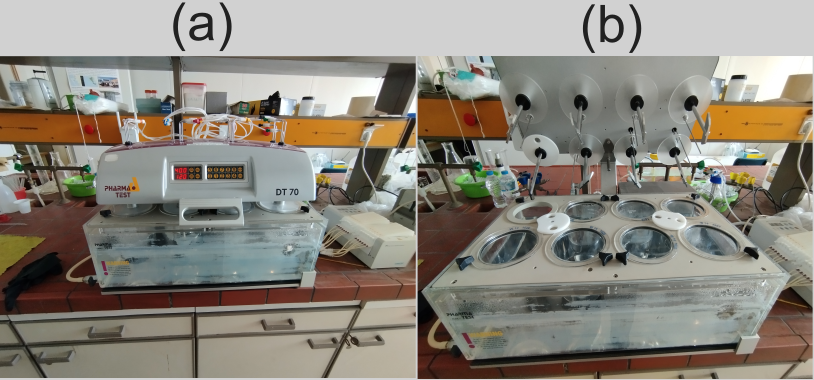
\includegraphics[width=.9\linewidth]{./lab_scale_hydrolysis.png}
\caption{\label{fig:orgfce8f3a}Πειραματική Διάταξη Υδρόλυσης Εργαστηριακής Κλίμακας}
\end{figure}

Συγκεκριμένα, το σύστημα αυτό αποτελείται από 7 ανεξάρτητα δοχεία χωρητικότητας 1 L, τα οποία είναι τοποθετημένα σε υδατόλουτρο για ρύθμιση της θερμοκρασίας και είναι εξοπλισμένα με αναδευτήρες τύπου κουπιού (Σχήμα \ref{fig:orgfce8f3a} (b)). Η θερμοκρασία και η ανάδευση ρυθμίζονται από μία οθόνη την οποία διαθέτει το μηχάνημα (Σχήμα \ref{fig:orgfce8f3a} (a)).  

Ένα από τα βασικά πλεονεκτήματα μίας τέτοιας διάταξης είναι η ευκολία να δοκιμαστούν ταυτόχρονα πολλές λειτουργικές συνθήκες, καθώς το κάθε δοχείο λειτουργεί ανεξάρτητα. Έτσι, είναι η ιδανική διάταξη για την βελτιστοποίηση μίας τέτοιας διεργασίας. Ένα μειονέκτημα της διάταξης είναι ότι δεν μπορεί να λειτουργήσει πλήρως αναερόβια, κάτι το οποίο θα ήταν επιθυμητό, καθώς η οξεογένεση είναι μία αναερόβια δράση. Όμως, με βάση την βιβλιογραφία (\autoref{sec:bacterial-enzymes}), τα υδρολυτικά και οξεογενετικά βακτήρια, όπως αυτά που έχουν επιλεχθεί στη παρούσα μελέτη, είναι προαιρετικά αναερόβια και μάλιστα υπάρχει αρκετή έρευνα γύρω από το αντικείμενο του μικροαερισμού, δηλαδή της προσθήκης μικρής ποσότητας οξυγόνου στην πρώτη φάση μίας αναερόβιας χώνευσης δύο σταδίων. Συγκεκριμένα, έχει παρατηρηθεί πως η προσθήκη αυτή βελτιώνει την μικροβιακή ποικιλότητα του αντιδραστήρα, αυξάνει την απόδοση της υδρόλυσης και δεν δημιουργεί προβλήματα στο επερχόμενο στάδιο της μεθανογένεσης, το οποίο είναι υποχρεωτικά αναερόβιο \textsuperscript{\citeprocitem{43}{43},\citeprocitem{57}{57}} . Οπότε, θεωρήθηκε πως δεν ήταν πρόβλημα να μπαίνει οξυγόνο στον αντιδραστήρα όποτε άνοιγε το καπάκι για δειγματοληψία.

\section{Δοκιμαστικά πειράματα υδρόλυσης}
\label{sec:orge81145e}
\label{sec:prep-hydro}

Για να αποφανθούν οι σημαντικότερες συνθήκες λειτουργίας της διεργασίας υδρόλυσης/βιοαποδόμησης έγιναν κάποια δοκιμαστικά πειράματα.

Το πρώτο δοκιμαστικό πείραμα χρησιμοποίησε τα \acrfull{ss} και το \acrfull{scod} ως βασικές αποκρίσεις. Η λογική αυτού ήταν πως τα \acrshort{ss} θα πρέπει να μειώνονται καθώς γίνεται υδρόλυση, ενώ δεν θα επηρεάζονται από αυξήσεις που οφείλονται στην ανάπτυξη των μικροοργανισμών και το \acrshort{scod} θα αυξάνεται καθώς γίνεται υδρόλυση και η στερεή οργανική ύλη διαλύεται. Εξετάστηκαν διαφορετικές αναλογίες \acrshort{fw}-νερού (1:1, 1:2 και 1:3), κρατώντας την ποσότητα \acrshort{fw} σταθερή στα 200 g, για να βρεθεί αν το μείγμα παραμένει ομοιογενές και μπορεί να παρατηρηθεί ικανοποιητική υδρόλυση. Η ανάδευση ρυθμίστηκε στα 120 rpm, όπου παρατηρήθηκε πως όλα τα μίγματα αναδευόντουσαν αποτελεσματικά. Η θερμοκρασία ρυθμίστηκε στους 45 \(^oC\), καθώς οι διεργασίες ενζυμικής υδρόλυσης είναι συνήθως αποδοτικές σε θερμοκρασίες κοντά στους 50 \(^oC\). 

Διαπιστώθηκε πως τα \acrfull{ss} μειώνονται σε 24 ώρες, αλλά και το \acrshort{scod} μειώθηκε. Έτσι, προέκυψε το συμπέρασμα πως η υδρόλυση και η ζύμωση διεξάγονται ταυτόχρονα και η ζύμωση έχει γρηγορότερο ρυθμό (εφόσον υπάρχει μείωση στερεών αλλά και μείωση \acrshort{scod}). Επίσης, παρατηρήθηκαν προβλήματα στην διεξαγωγή της διήθησης στις αραιώσεις 1:1 και 1:2, οπότε για όλα τα επόμενα πειράματα χρησιμοποιήθηκε η αραίωση 1:3.

Για να μελετηθεί πιο αναλυτικά η αλληλεπίδραση των δύο διεργασιών και να επιλεχθούν οι κατάλληλες συνθήκες για έναν πειραματικό σχεδιασμό βελτιστοποίησης, έγινε ένα δεύτερο πείραμα. Στο πείραμα αυτό χρησιμοποιήθηκαν 2 επαναλήψεις του ίδιου πειράματος (για να μελετηθεί η επαναληψιμότητα της διεργασίας), στο οποίο χρησιμοποιήθηκε αναλογία \acrshort{fw}-νερού 1:3 και ανάδευση 120 rpm, όπως επιλέχθηκαν από το προηγούμενο πείραμα. Η θερμοκρασία ρυθμίστηκε στους 45 \(^oC\) και προστέθηκαν 2 mL \acrshort{mix}. Ως μεταβλητές απόκρισης, δοκιμάστηκαν οι εξής: \acrshort{ss} (ολικά και πτητικά), \acrshort{scod}, συγκέντρωση σακχάρων και συγκέντρωση προϊόντων οξεογενούς ζύμωσης (συγκεκριμένα μετρήθηκαν γαλακτικό οξύ, οξικό οξύ, προπιονικό οξύ και αιθανόλη). Για να αποφασισθεί η διάρκεια της διεργασίας υδρόλυσης/βιοαποδόμησης, η δειγματοληψία στο πείραμα αυτό ήταν συχνή. Συγκεκριμένα, την πρώτη μέρα έγινε δειγματοληψία στις 0, 1, 2, 3, 4, 5, 6 ενώ τις επόμενες 4 ημέρες, γινόταν δειγματοληψία κάθε 2 ώρες για 6 ώρες. Στο 2ο δείγμα (που χρησιμοποιείται για επανάληψη) δεν έγιναν οι συχνές δειγματοληψίες την πρώτη μέρα, αλλά μόνο δειγματοληψίες στις 0, 1 και 5 ώρες. Καθώς παρατηρήθηκαν αλλαγές μέχρι και την 5η μέρα (98 ώρες), το πείραμα αυτό αφέθηκε να λειτουργήσει και πάρθηκαν 2 τελευταία δείγματα στις 167 και 171 ώρες για να διαπιστωθεί αν θα παρατηρηθεί κάποιο πλατό.

Τέλος, έγινε ένα τρίτο πείραμα, όπου μετρήθηκε κατά βάση η εξάτμιση του νερού, η οποία παρατηρήθηκε πως έπαιξε σημαντικό ρόλο στα προηγούμενα πειράματα. Συγκεκριμένα, καθώς η διάταξη που χρησιμοποιήθηκε έχει 7 θέσεις, τοποθετήθηκαν 7 πανομοιότυπα πειράματα με τις εξής συνθήκες: 200 g \acrshort{fw}, 600 g νερό, 2 mL \acrshort{mix}, θερμοκρασία ρυθμισμένη στους 35 \(^oC\) και ανάδευση στα 120 rpm. Μετά από 1, 2, 3, 7, 9, 11 και 14 ημέρες μετά την έναρξη του πειράματος, ένα από τα 7 δείγματα αφαιρούταν από την διάταξη και μετριόταν η μάζα του καθώς και τα TS του. Αφαιρώντας την μείωση μάζας των στερεών (η οποία οφείλεται καθαρά στην υδρόλυση) από την μείωση της συνολικής υγρής μάζας, μπόρεσε να προσδιοριστεί η μείωση της μάζας του νερού. Εφόσον δεν υπήρχαν δειγματοληψίες, η απώλεια μάζας αυτή οφειλόταν αποκλειστικά στην εξάτμιση. Έτσι, ποσοτικοποιήθηκε και ο ρυθμός εξάτμισης.

\section{Πειραματικός κύκλος υδρόλυσης}
\label{sec:orgce47dfd}
\label{sec:lab-hydro}
Με βάση τα αποτελέσματα των δοκιμαστικών πειραμάτων αυτών σχεδιάστηκε ένας πειραματικός κύκλος για την βελτιστοποίηση της διεργασίας. Αποφασίστηκε να μην ρυθμιστεί η αραίωση και η ανάδευση και να αφεθούν στην τιμή που βρέθηκε πως λειτουργεί καλά η διεργασία (200 mL \acrshort{fw}, 600 mL νερό, 120 rpm ανάδευση), ενώ ως παράμετροι προς βελτιστοποίηση επιλέχθηκαν η θερμοκρασία και η ποσότητα του \acrshort{mix}. Για την θερμοκρασία, εξετάστηκαν οι τιμές 35 και 40 \(^oC\) ως δύο αντιπροσωπευτικές τιμές της μεσόφιλης περιοχής, ενώ όπου υπήρχε η δυνατότητα, εξετάστηκε και η διαφορά τους με την θερμοκρασία 45 \(^oC\) όπου έγινε ένα από τα δοκιμαστικά πειράματα. Για την ποσότητα του \acrshort{mix} εξετάστηκαν οι τιμές 0 (επίδραση μόνο της θερμοκρασίας), 1, 2, 4 και 8 ml ανά 200 mL FW. 

Ως μεταβλητές απόκρισης στα πειράματα αυτά επιλέχθηκαν η μέτρηση των συγκεντρώσεων σακχάρων, των \acrshort{vfa} και του \acrshort{scod}.  Με αυτά, μπορούν να υπολογιστούν τα εξής: η συνολική συγκέντρωση \acrshort{vfa} η οποία δείχνει πόσα προϊόντα παράχθηκαν και ιδιαίτερα ο λόγος \(\frac{\text{tVFAs in COD-eq}}{\text{sCOD}}\) ο οποίος είναι ένας πολύ χρήσιμος λόγος για μία διεργασία οξεογένεσης καθώς αποτελεί την απόδοση της. Επίσης, σημαντική είναι και η αναλογία της τελικής υγρής απορροής στα διάφορα \acrshort{vfa}, η οποία είναι καθοριστική για την ποιότητα της αναερόβια χώνευση.

Εκτός από την τελική δειγματοληψία όμως, έγιναν και δειγματοληψίες κατά την διάρκεια του πειράματος (μία φορά την ημέρα, η οποία κρίθηκε η βέλτιστη συχνότητα μετά τα δοκιμαστικά πειράματα). Η δειγματοληψία αυτή επέτρεψε την καταγραφή κάποιων σταδίων στην διεργασία, το οποίο επέτρεψε την διαπίστωση των μεταβολικών μονοπατιών που ακολουθήθηκαν.

\section{Υδρόλυση σε πιλοτική κλίμακα}
\label{sec:org3288570}
\label{sec:pilot-exp}

Για τα πειράματα σε πιλοτική κλίμακα χρησιμοποιήθηκε ο πρωτότυπος αερόβιος χωνευτήρας (MyECO) χωρητικότητας 300 L. Η διάταξη αυτού φαίνεται στο Σχήμα \ref{fig:org4b33ff5}.

\begin{figure}[htbp]
\centering
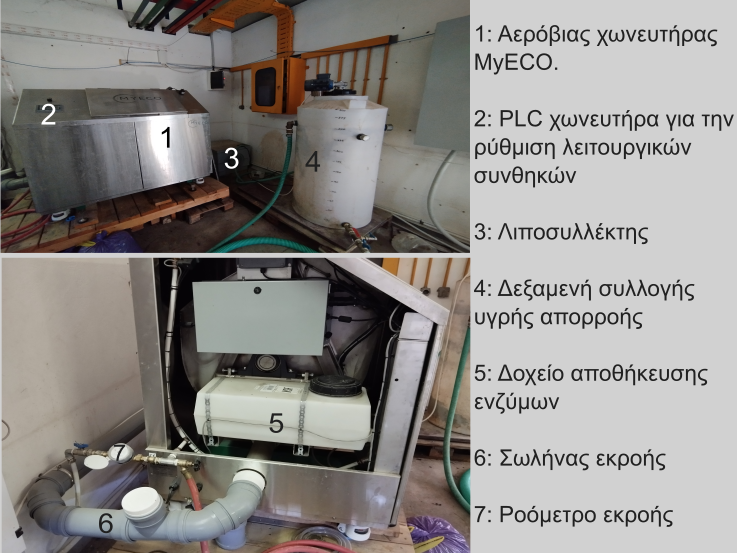
\includegraphics[width=.9\linewidth]{./pilot_hydrolysis_captioned.png}
\caption{\label{fig:org4b33ff5}Πειραματική Διάταξη Πιλοτικής Υδρόλυσης}
\end{figure}

Στο εσωτερικό του χωνευτήρα έχει τοποθετηθεί αδρανές πλαστικό πληρωτικό υλικό, για την καλύτερη διεπαφή \acrshort{fw} και ενζύμων-μικροοργανισμών καθώς και τον σχηματισμό βιοφίλμ, ο οποίος ανεβάζει την απόδοση επεξεργασίας της χώνευσης. Ακόμη, στο εσωτερικό του χωνευτήρα υπάρχει ένας οριζόντιος άξονας με 4 ράβδους οι οποίες επιτρέπουν τον τεμαχισμό και ταυτόχρονα την ανάδευση του συστήματος. Συγκεκριμένα, οι ράβδοι αυτές έχουν ελαστικά άκρα, όποτε μπορούν να τεμαχίσουν τα υδρολύματα κατά την περιστροφή τους και να τα μεταφέρουν προς την εκροή, αναδεύοντας τα. Το σύστημα αυτό έχει ισχύ 1 HP. Επιπλέον, ο χωνευτήρας διαθέτει εσωτερική ζυγαριά για την μέτρηση της μάζας της τροφοδοσίας και ενσωματωμένο PLC (2) που επιτρέπει την ρύθμιση του ρυθμού τροφοδοσίας του σκευάσματος, το οποίο είναι αποθηκευμένο σε ειδικό δοχείο του οργάνου (5), καθώς και του νερού που προστίθεται στο εσωτερικό του αντιδραστήρα, αλλά και στην εκροή του, για την αραίωση του τελικού προϊόντος. Μετά από κάποιον χρόνο παραμονής, η επεξεργασμένη υγρή εκροή αποβάλλεται από τον χωνευτήρα (6) και οδηγείται σε λιποσυλλέκτη (3) για να απομακρυνθούν οι λιπαρές ενώσεις. Η εκροή αυτού οδηγείται στη δεξαμενή συλλογής χωρητικότητας 300 L (4) από την οποία γίνεται η δειγματοληψία για να αναλυθεί η ποιότητα της εκροής αυτής. Το όργανο διαθέτει ροόμετρο για την μέτρηση της εκροής του (7).

Η λειτουργία του είναι ήμι-διαλείποντος έργου καθώς ο αντιδραστήρας τροφοδοτείται 2 φορές την ημέρα (μία το πρωί και μία το απόγευμα) ενώ η εκροή του λειτουργεί συνεχώς.

Τα πειράματα που διεξάχθηκαν στην κλίμακα αυτή είχαν ως σκοπό να εξετάσουν την εφικτότητα της υδρόλυσης σε μεγαλύτερη κλίμακα και την συλλογή υδρολύματος για αναερόβια χώνευση, για να διαπιστωθεί αν αυτή είναι το ίδιο αποτελεσματική στην εργαστηριακή και πιλοτική κλίμακα. Για τον σκοπό αυτόν, η τροφοδοσία του \acrshort{mix} ρυθμίστηκε σε τιμές οι οποίες αντιστοιχούν στις αναλογίες που χρησιμοποιήθηκαν στα πειράματα εργαστηριακής κλίμακας. Βέβαια, ο πιλοτικός χωνευτήρας δεν έχει την δυνατότητα ελέγχου της θερμοκρασίας, οπότε αναμένεται να μην είναι ακριβώς ίδια η ζύμωση σε σχέση με αυτήν στην εργαστηριακή κλίμακα. Για να εξεταστεί κάποια άλλη λειτουργική συνθήκη του συστήματος, έγινε ένας πειραματικός κύκλος όπου αυξήθηκε η προσθήκη νερού στον χωνευτήρα, για να διαπιστωθεί αν θα επηρεάσει πραγματικά το σύστημα, ή αν θα μειώσει απλώς το \acrshort{cod} λόγω αραίωσης.

Οπότε, οι 3 κύκλοι οι οποίοι διεξάχθηκαν είχαν τις εξής συνθήκες:
\begin{itemize}
\item 1ος κύκλος (P1): Τροφοδοσία 35.8 kg \acrshort{fw}/day με προσθήκη 4.24 L νερό/kg \acrshort{fw} και 0.005 L \acrshort{mix}/kg \acrshort{fw} (αντίστοιχο με το 1 mL στην εργαστηριακή κλίμακα).
\item 2ος κύκλος (P2): Τροφοδοσία 37.5 kg \acrshort{fw}/day με προσθήκη 5.71 L νερό/kg \acrshort{fw} και 0.005 L \acrshort{mix}/kg \acrshort{fw}.
\item 3ος κύκλος (P3): Τροφοδοσία 24.9 kg \acrshort{fw}/day με προσθήκη 8.9 L νερό/kg \acrshort{fw} και 0.01 L \acrshort{mix}/kg \acrshort{fw} (αντίστοιχο με το 2 mL στην εργαστηριακή κλίμακα).

Αξίζει να αναφερθεί πως το νερό είναι σε κάθε περίπτωση περισσότερο από αυτό που χρησιμοποιούταν στα πειράματα εργαστηριακής κλίμακας (3 L νερό/kg \acrshort{fw}). Αυτό συμβαίνει διότι στην πιλοτική διάταξη απαιτείται περισσότερο νερό για να είναι ομοιογενής η λειτουργία και να μην υπάρχουν προβλήματα από ότι στην εργαστηριακή κλίμακα.

Ως απόκριση της διεργασίας, εξετάστηκαν οι παραμέτροι \acrshort{ts}, \acrshort{vs}, \acrshort{scod}, \acrshort{tcod} . Ιδιαίτερα σημαντικό για την διεργασία θεωρήθηκε να είναι υψηλή η αναλογία sCOD/tCOD, η οποία αποτελεί την απόδοση της διεργασίας υδρόλυσης/βιοαποδόμησης.
\end{itemize}

\section{Πειραματική διάταξη αναερόβιας χώνευσης}
\label{sec:org80eebd6}
Η \acrshort{ad} πραγματοποιήθηκε σε εργαστηριακούς αντιδραστήρες διαλείποντος έργου, συνολικού όγκου 500 mL ο καθένας. Η διάταξη που χρησιμοποιήθηκε φαίνεται στο Σχήμα \ref{fig:org1fc0a68}.

\begin{figure}[htbp]
\centering
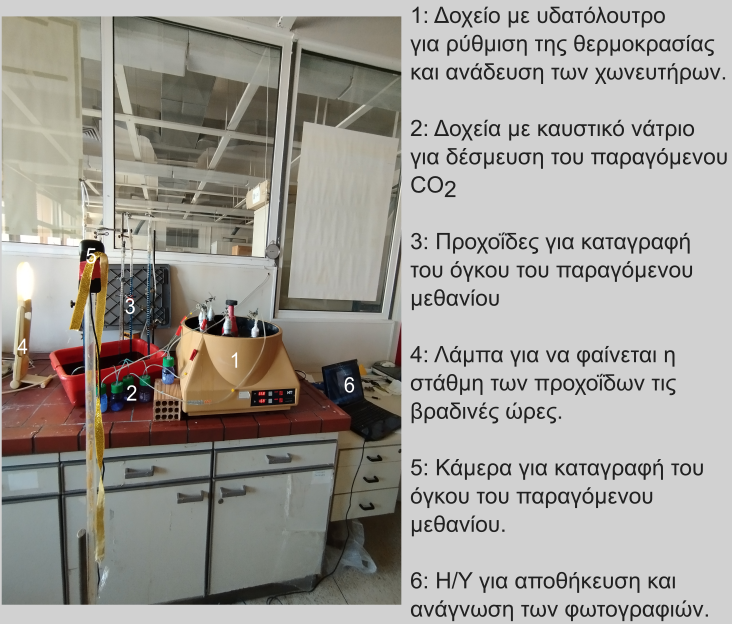
\includegraphics[width=350px]{./anaerobic_digestion_captioned.png}
\caption{\label{fig:org1fc0a68}Πειραματική Διάταξη Αναερόβιας Χώνευσης}
\end{figure}

Για να διεξαχθεί ένας κύκλος πειραμάτων αναερόβιας χώνευσης, αρχικά ανοίγει το υδατόλουτρο (1) για να φτάσει την επιθυμητή θερμοκρασία και πληρώνονται οι αντιδραστήρες με λάσπη και νερό. Σφραγίζονται με χρήση parafilm και σιλικόνης για να είναι σίγουρο ότι δεν θα μπορέσει να υπάρξει κάποια διαρροή, δηλαδή απώλεια μεθανίου. Για να εκκινήσει η αντίδραση, το υπόστρωμα τροφοδοτείται στον αντιδραστήρα από ειδικό σωληνάκι με χρήση σύριγγας. Μόλις παραχθεί αέριο, αυτό θα διοχετευθεί στα δοχεία με το καυστικό νάτριο (2). Το καυστικό νάτριο μπορεί να δεσμεύσει το διοξείδιο του άνθρακα καθώς αντιδρά με το ανθρακικό οξύ που παράγεται όταν το CO\textsubscript{2} βρεθεί σε υδατική φάση. Ως αποτέλεσμα, στις προχοΐδες (3) διοχετεύεται καθαρό μεθάνιο, το οποίο είναι και αυτό που μας ενδιαφέρει. Η κάμερα (5) καταγράφει μία φορά την ώρα την στάθμη του νερού όλο το 24 ώρο, για να μπορέσει να γίνει μία κινητική μελέτη της διεργασίας αναερόβιας χώνευσης. Για τις βραδινές ώρες, είναι απαραίτητο να είναι ανοιχτή η λάμπα (4), ώστε να μπορεί να διαβαστεί η στάθμη των προχοΐδων. Οι φωτογραφίες που βγαίνουν κάθε ώρα, αποθηκεύονται στον Η/Υ (6), για να μπορέσουν να αναγνωστούν.

Έτσι, με την διάταξη αυτή μπορεί να εξεταστεί εύκολα το \acrfull{bmp} 5 διαφορετικών υποστρωμάτων ταυτόχρονα καθώς και ο ρυθμός παραγωγής μεθανίου σε αυτά ή η \acrfull{sma} τους. 

\section{Πειραματικός κύκλος αναερόβιας χώνευσης}
\label{sec:orge34a15f}
\label{sec:exp-ad}

Μετά από βελτιστοποίηση της υδρόλυσης στην εργαστηριακή κλίμακα, αποφασίστηκε πως η θερμοκρασία 40 \(^oC\) είναι πιο αποτελεσματική και ότι οι ποσότητες 1, 2 και 4 έχουν τα καλύτερα αποτελέσματα και αξίζει να διερευνηθούν περαιτέρω. Οπότε, οι 2 πρώτοι πειραματικοί κύκλοι αναερόβιας χώνευσης έγιναν με τα υδρολύματα αυτά για να εξεταστεί η ικανότητα τους να παράξουν μεθάνιο. Έπειτα, έγινε και ένας τρίτος κύκλος στον οποίο εξετάστηκε η ικανότητα παραγωγής μεθανίου από τα υδρολύματα που προήλθαν από την πιλοτική υδρόλυση. Σε όλα τα πειράματα η θερμοκρασία ήταν ρυθμισμένη στους 37 \(^oC\) και η ανάδευση στα 170 rpm.

Κατά τον πρώτο κύκλο πειραμάτων, ο οποίος διεξάχθηκε με την Λάσπη 1, χρησιμοποιήθηκε εμβόλιο 125 g λάσπης (1.55 g VS/αντιδραστήρα) και πλήρωση του αντιδραστήρα με νερό. Αρχικά, η αναερόβια λάσπη ενεργοποιήθηκε με τροφοδοσία οξικού οξέος (100 mg), και στη συνέχεια, ακολούθησε η τροφοδοσία με τα υδρολύματα. Εκτός από τα υδρολύματα με 1, 2 και 4 mL \acrshort{mix}/200 g \acrshort{fw}, χρησιμοποιήθηκαν και το δείγμα με 0 mL \acrshort{mix}, το οποίο δείχνει την επίδραση μόνο της θερμοκρασίας, και το ανεπεξέργαστο \acrshort{fw}, για να διαπιστωθεί αν η αναερόβια χώνευση πραγματικά βελτιώνεται με την προσθήκη του \acrshort{mix}. Η τροφοδοσία με υδρολύματα έγινε με 100 mg \acrshort{scod}, δηλαδή μία αναλογία \acrfull{si} 0.06 g COD/g VS. Η αναλογία αυτή είναι σχετικά μικρή σε σχέση με άλλες μελέτες \textsuperscript{\citeprocitem{32}{32},\citeprocitem{76}{76},\citeprocitem{97}{97}}. Η επιλογή αυτή έγινε επειδή έτσι υπάρχει μία πιο άμεση απόκριση στα πειράματα και άρα μπορεί ο χρόνος διεξαγωγής τους να περιοριστεί σε περίπου μία βδομάδα, κάτι το οποίο επιτρέπει την εκτέλεση πολλών πειραματικών κύκλων. Επιπλέον, υπήρχε και ένας περιορισμός από την διάταξη, η οποία είχε προχοΐδες των 50 mL, οπότε αν η παραγωγή μεθανίου ήταν πολύ περισσότερη από αυτή την ποσότητα, θα ήταν δύσκολο να καταγραφεί.

Ο δεύτερος κύκλος πειραμάτων έγινε με παρόμοια λογική. Σκοπός ήταν να εξεταστεί αναερόβια λάσπη από διαφορετική πηγή (Λάσπη 2), για να διαπιστωθεί αν υπάρχει επαναληψιμότητα στα πειράματα. Στον κύκλο αυτό προστέθηκε μεγαλύτερο εμβόλιο λάσπης (250 g ή 4.2 g VS) ενώ η ποσότητα των υδρολυμάτων παρέμεινε ίδια (100 mg \acrshort{scod}). Οπότε, η αναλογία \acrshort{si} ήταν 0.02 g COD/g VS.

Στον τρίτο κύκλο χρησιμοποιήθηκαν τα υδρολύματα της πιλοτικής μονάδας. Συγκεκριμένα, χρησιμοποιήθηκαν τα πειράματα P1 και P3, τα οποία ήταν σε ποσότητα \acrshort{mix} ισοδύναμα των πειραμάτων με 1 και 2 ml \acrshort{mix} από την εργαστηριακή κλίμακα. Σκοπός του κύκλου αυτού ήταν να επιβεβαιωθεί η εφικτότητα της παραγωγής μεθανίου από το υδρόλυμα αυτό και η διαφορές που έχει από τα ίδια πειράματα σε εργαστηριακή κλίμακα. Καθώς όμως εξετάστηκαν μόνο 2 υδρολύματα, υπήρξε δυνατότητα να χρησιμοποιηθεί λάσπη από 2 διαφορετικές πηγές στον ίδιο κύκλο, για να διαπιστωθεί η επαναληψιμότητα αυτού. Συγκεκριμένα, χρησιμοποιήθηκε η Λάσπη 2 για να συγκριθούν τα αποτελέσματα με την εργαστηριακή κλίμακα, αλλά χρησιμοποιήθηκε επίσης και η Λάσπη 3. Και στις 2 περιπτώσεις χρησιμοποιήθηκαν 250 g λάσπης, αλλά αυτό ισοδυναμεί σε 4.2 g VS για την Λάσπη 2 και σε 0.5 g VS για την Λάσπη 3.

Ως βασικές αποκρίσεις εδώ, χρησιμοποιήθηκαν η μέγιστη παραγωγή μεθανίου από κάθε δείγμα, καθώς και ο ρυθμός παραγωγής αυτού με βάση το τροποποιημένο μοντέλο Gompertz (\autoref{sec:gompertz}) εφόσον υπήρχε η δυνατότητα 24ωρής καταγραφής του φαινομένου.

\section{Αναλυτικές Μέθοδοι}
\label{sec:org44157e4}
\label{sec:analyses}

Η μέτρηση pH έγινε με χρήση pH μέτρου (inoLab pH Level 1 pH Meter) σε ακολουθία με τις πρότυπες τεχνικές, ενότητα 4500-H\^{}+ \textsuperscript{\citeprocitem{101}{101}}. Η μέτρηση ηλεκτρικής αγωγιμότητας έγινε με τον ηλεκτροχημικό αναλυτή CONSORT C933.

Η μέτρηση των στερεών, έγινε σε ακολουθία με τις πρότυπες τεχνικές, ενότητα 2540 \textsuperscript{\citeprocitem{101}{101}} . Συγκεκριμένα για τα \acrfull{ts}, έγινε ζύγιση σε προ-ζυγισμένη κάψα μετά από ξήρανση σε φούρνο στους 75 \(^oC\) για 1 μέρα, ενώ για να μετρηθούν τα \acrfull{vs}, έγινε ζύγιση μετά από ξήρανση σε φούρνο στους 550 \(^oC\) για 2 ώρες. Για τα \acrfull{ss}, έγινε αρχικά διήθηση του δείγματος με χρήση προ-ζυγισμένου φίλτρου Whatman GF/A το οποίο κατακρατεί στερεά διαμέτρου 1.6 μm και πάνω. Έπειτα, ακολουθήθηκε η ίδια διαδικασία με παραπάνω για την μέτρηση ολικών και πτητικών αιωρουμένων στερεών.

Η μέτρηση του \acrshort{cod} έγινε σε ακολουθία με τις πρότυπες τεχνικές, ενότητα 5220 \textsuperscript{\citeprocitem{101}{101}}. Για την μέτρηση αυτή, αρχικά γίνεται αραίωση του δείγματος ανάλογα με το αναμενόμενο \acrshort{cod}, καθώς η μέθοδος είναι αξιόπιστη σε COD από 50 έως 1000 mg/L. Έπειτα, 2 ml του αραιωμένου δείγματος αναμιγνύονται με 2.8 ml πυκνού θειικού οξέος και 1.2 ml διχρωμικού καλίου και τοποθετούνται σε ειδικό φούρνο στους 150 \(^oC\) για 2 ώρες (HACH COD Reactor 45600). Το διχρωμικό κάλιο είναι ισχυρό οξειδωτικό, ενώ το θειικό οξύ και η θερμοκρασία δρουν ως καταλύτες της αντίδρασης. Ανάλογα με το \acrshort{cod}, μεταβάλλεται η οξειδωτική κατάσταση του χρωμίου από +6 σε +3. Ταυτόχρονα, μεταβάλλεται το χρώμα του από πορτοκαλί σε γαλάζιο. Μετρώντας την απορρόφηση στα 600 nm μετά τις 2 ώρες, μπορεί να ποσοτικοποιηθεί η οξείδωση που διεξάχθηκε, και άρα το COD του δείγματος. Για να μετρηθεί το \acrshort{cod} ενός δείγματος, απαιτείται μία πρότυπη καμπύλη η οποία αντιστοιχεί την απορρόφηση σε συγκέντρωση \acrshort{cod}. Για την μέτρηση του \acrshort{tcod} το δείγμα λαμβανόταν ως είχε, ενώ για την μέτρηση του \acrshort{scod}, το δείγμα αρχικά διηθούταν με χρήση φίλτρου Whatman. Για ορισμένα δείγματα με πολλά στερεά, γινόταν και μία φυγοκέντριση (EBA 20, Hettich Zentrifugen σε συνθήκες 6000 rpm, 10 λεπτά) για να ολοκληρωθεί πιο γρήγορα ο διαχωρισμός των στερεών.

Για την αλκαλικότητα ακολουθήθηκε η μέθοδος της ογκομέτρησης. Συγκεκριμένα, 20 mL δείγματος ογκομετρήθηκαν με θειικό οξύ κανονικότητας 0.2 Ν μέχρι το pH να φτάσει 4.5. Ο όγκος που απαιτείται (V\textsubscript{sulf}) είναι ενδεικτικός της αλκαλικότητας. Συγκεκριμένα, ισχύει \(\text{Alkalinity} = \frac{50 \cdot 1000 \cdot 0.2 \cdot V_{sulf}}{20}\) με την αλκαλικότητα να μετριέται σε mg CaCO\textsubscript{3}/L.  

Για την μέτρηση των σακχάρων και των πτητικών λιπαρών οξέων κατά την υδρόλυση, χρησιμοποιήθηκε μία στήλη για \acrfull{hplc} (Agilent Technologies Infinity II). Ακολουθήθηκε η μέθοδος lactic temp, η οποία έχει χρόνο παραμονής στην στήλη 45 λεπτά και κινητή φάση HPLC Grade νερό με πυκνό θεϊικό οξύ συγκέντρωσης 275 μL/L. Οι κορυφές που ταυτοποιήθηκαν είναι για τις εξής ενώσεις: γλυκόζη, φρουκτόζη, σακχαρόζη, γαλακτικό οξύ, οξικό οξύ, προπιονικό οξύ και αιθανόλη. Στα χρωματογραφήματα υπήρχαν και κάποιες άλλες κορυφές, αλλά ήταν πολύ μικρές και θεωρήθηκαν αμελητέες. Οι κορυφές που ταυτοποιήθηκαν δεν παρουσίασαν κάποια επικάλυψη και ήταν όλες αρκετά ψηλές για να είναι έμπιστη η μέτρηση τους.

\chapter{Επεξεργασία Αποτελεσμάτων}
\label{sec:orga8c48e7}
\label{sec:result_analysis}

Όλα τα πειραματικά αποτελέσματα αναλύθηκαν με την βοήθεια της γλώσσας προγραμματισμού Julia \textsuperscript{\citeprocitem{102}{102}}. Η Julia είναι μία ελεύθερα διαθέσιμη γλώσσα η οποία είναι ιδιαίτερα κατάλληλη για υπολογιστικά προβλήματα όπως αυτά που χρειάστηκε να αναλυθούν. Η είσοδος και έξοδος δεδομένων μπορεί να γίνει εύκολα μέσω αρχείων CSV με την χρήση βιβλιοθηκών όπως οι CSV.jl και DataFrames.jl \textsuperscript{\citeprocitem{103}{103}}, κάτι το οποίο επιτρέπει την δια-λειτουργικότητα με εργαλεία όπως το Microsoft Office Excel το οποίο μπορεί να δημιουργήσει αλλά και να διαβάσει τα αρχεία αυτά. Ακόμη, έχει πολύ καλές δυνατότητες παρουσίασης αποτελεσμάτων λόγω των εξαιρετικών βιβλιοθηκών της για γραφήματα. Στην εργασία αυτή χρησιμοποιήθηκαν τα \textsuperscript{\citeprocitem{104}{104},\citeprocitem{105}{105}} . Η ανάλυση των αποτελεσμάτων έγινε με επαναλήψιμο τρόπο με την βοήθεια της βιβλιοθήκης DrWatson \textsuperscript{\citeprocitem{106}{106}} και ανέβηκε στο \href{https://github.com/Vidianos-Giannitsis/masters-thesis}{GitHub}. Έτσι, κάνοντας clone το repository αυτό, μπορεί οποιοσδήποτε να αναπαράγει τα αποτελέσματα που θα παρουσιαστούν.

Σκοπός του κεφαλαίου αυτού είναι μία παρουσίαση του τρόπου επεξεργασίας των πειραματικών αποτελεσμάτων της εργασίας και παράθεση των βασικών αποτελεσμάτων ενώ στο επόμενο κεφάλαιο θα γίνει ο σχολιασμός αυτών καθώς και η παράθεση κάποιων συγκεντρωτικών αποτελεσμάτων από τα οποία προκύπτουν άμεσα τα τελικά συμπεράσματα.

\section{Δοκιμαστικά πειράματα υδρόλυσης}
\label{sec:org9308642}
Τα πρώτα πειράματα που έγιναν ήταν τα δοκιμαστικά πειράματα για την υδρόλυση \autoref{sec:prep-hydro}. Αυτά επέτρεψαν την διαπίστωση των βέλτιστων συνθηκών λειτουργίας για τον κύριο πειραματικό κύκλο της υδρόλυσης.

\begin{enumerate}
\item Δοκιμή Διάφορων Αραιώσεων:
\label{sec:org20d5127}
Από το πρώτο πείραμα δεν προέκυψαν πολλά αποτελέσματα, πέρα από το γεγονός ότι υδρόλυση και ζύμωση διεξάγονται ταυτόχρονα με την ζύμωση να υπερισχύει. Αξίζει να αναφερθεί πως από τα πειράματα που έγιναν, στην αραίωση 1:1 δεν μπόρεσε να διηθηθεί το δείγμα (και απορρίφθηκε γενικά ως αραίωση), στην αραίωση 1:2 ολοκληρώθηκε οριακά η διήθηση και στην αραίωση 1:3 διηθήθηκε κανονικά. Παρακάτω παρατίθενται τα διαγράμματα για τα \acrfull{tss} (\ref{fig:org56b12cb}) και το \acrfull{scod} (\ref{fig:org4e6c748}) για το πείραμα αυτό. Τα \acrfull{vss} μετρήθηκαν αλλά δεν παρουσιάζονται καθώς ακολουθούν ακριβώς την ίδια τάση με τα \acrfull{tss}. Συγκεκριμένα, για το πείραμα με αραίωση 1:2 ο λόγος VSS/TSS ήταν \(96.65 \pm 0.50\) και για την αραίωση 1:3 \(97.98 \pm 0.23\). 

\begin{figure}[htbp]
\centering
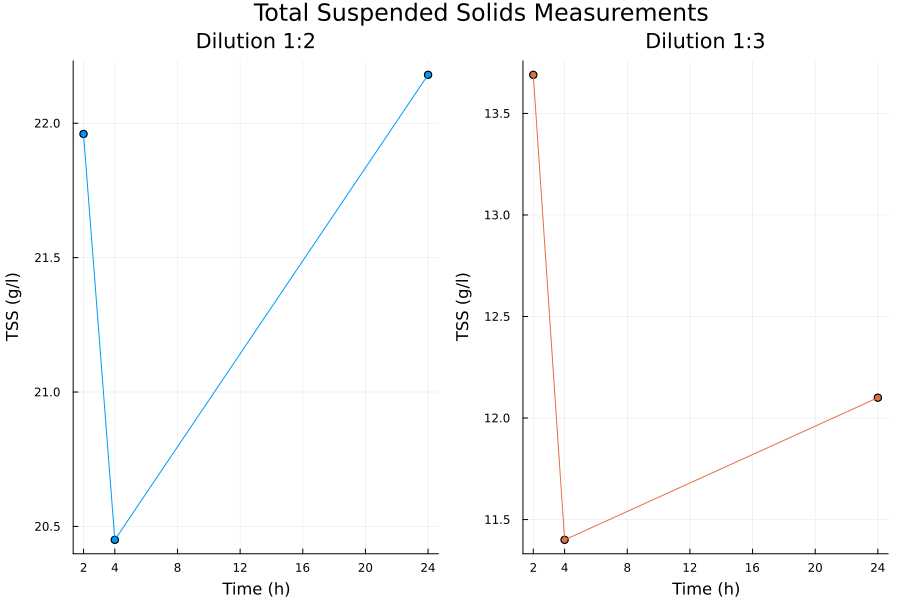
\includegraphics[width=.9\linewidth]{../plots/10_10/tss_plot.png}
\caption{\label{fig:org56b12cb}Μέτρηση TSS - Δοκιμαστικό Πείραμα 1}
\end{figure}

\begin{figure}[htbp]
\centering
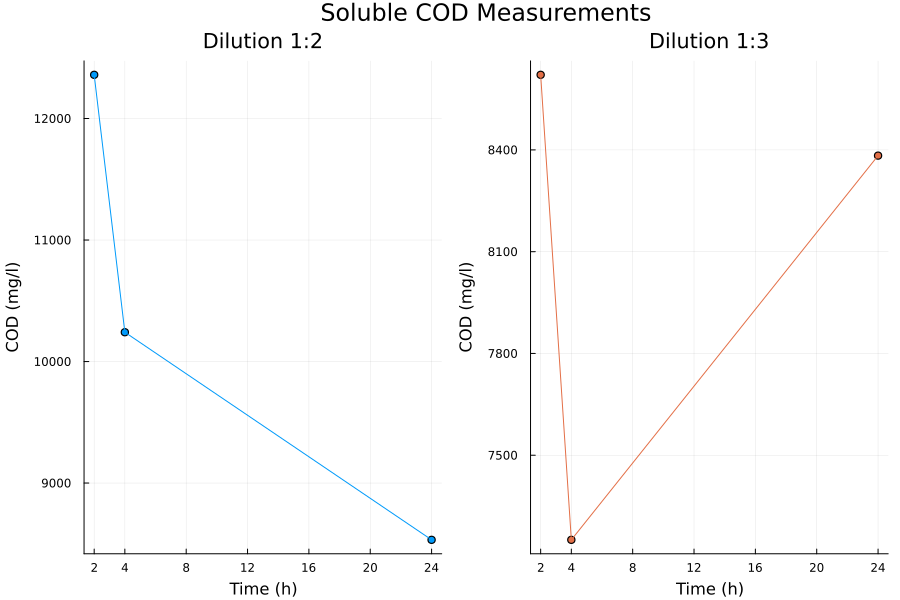
\includegraphics[width=.9\linewidth]{../plots/10_10/COD_plot.png}
\caption{\label{fig:org4e6c748}Μέτρηση Διαλυτού COD - Δοκιμαστικό Πείραμα 1}
\end{figure}

\item Αρχικό Κινητικό Πείραμα:
\label{sec:org70e75e1}
Το επόμενο πείραμα ήταν το δοκιμαστικό πείραμα κινητικής το οποίο έγινε στους 45 \(^oC\). Από το πείραμα αυτό μετρήθηκαν πολλές διαφορετικές αποκρίσεις για να διαπιστωθεί ποιες έχουν νόημα και ποιες όχι και επίσης έγινε συχνή δειγματοληψία.

Λόγω της πολύ μεγάλης διάρκειας του πειράματος και των συχνών δειγματοληψιών, παρατηρήθηκε πως η στάθμη του δοχείου στα 2 πειράματα μειώθηκε αρκετά (περίπου 550 ml ενώ ξεκίνησε από 800 ml). Η μεγάλη μεταβολή του όγκου, που οφείλεται σε μεγάλο βαθμό στην απώλεια νερού, επηρεάζει μάλλον και τις συγκεντρώσεις που μετρήθηκαν σε κάποιο βαθμό. Για αυτό και αποφασίστηκε η δειγματοληψία να γίνεται μία φορά την ημέρα για τα επόμενα πειράματα.

Συγκεκριμένα, η μέτρηση των ολικών και πτητικών αιωρουμένων στερεών θεωρείται πως δεν είναι αξιόπιστη καθώς παρουσιάζει έντονη παλινδρομική συμπεριφορά ενώ θεωρητικά δεν υπάρχει κάποια εξήγηση για την αύξηση των στερεών (πέρα από να επηρεάστηκαν από την μεταβολή του όγκου του νερού).

Μία αντίστοιχη παλινδρομική συμπεριφορά διαπιστώθηκε και στο \acrshort{cod}. Στην περίπτωση αυτή, παρότι σίγουρα επηρεάζεται και αυτό από τα παραπάνω προβλήματα, είναι πολύ πιο εύκολο να εξηγηθεί η παρουσία ταλαντώσεων. Εφόσον συμβαίνει ταυτόχρονα υδρόλυση και ζύμωση, η μία διεργασία αυξάνει το \acrshort{cod} ενώ η άλλη το μειώνει. Οι ρυθμοί αυτοί είναι δυναμικοί καθώς εξαρτώνται από πολλούς παράγοντες. Οπότε, παρόλο που από το \acrshort{cod} μπορεί να καταγραφεί μία ένδειξη του ποιος ρυθμός είναι και ο υψηλότερος την κάθε στιγμή, δεν θεωρείται η πιο καλή ανάλυση για την μελέτη της διεργασίας. Στο Σχήμα \ref{fig:org7ba1b83} φαίνονται τα αποτελέσματα της ανάλυσης αυτής.

\begin{figure}[htbp]
\centering
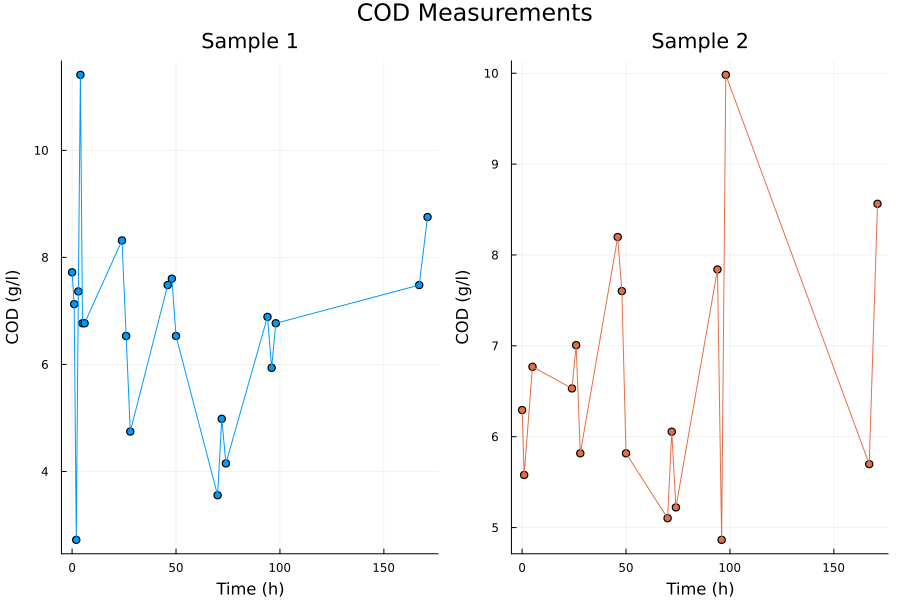
\includegraphics[width=.9\linewidth]{../plots/23_10/cod_scatter_23_10.png}
\caption{\label{fig:org7ba1b83}Μέτρηση COD - Αρχικό Κινητικό Πείραμα}
\end{figure}

Λόγω των προβλημάτων της ανάλυσης αυτής, αποφασίστηκε να γίνει μία πιο στοχευμένη ανάλυση. Από την βιβλιογραφία, είναι γνωστό πως η \acrfull{hplc} είναι μία αναλυτική μέθοδος η οποία μπορεί να ανιχνεύσει σάκχαρα, αλκοόλες και πτητικά λιπαρά οξέα \textsuperscript{\citeprocitem{37}{37},\citeprocitem{64}{64},\citeprocitem{107}{107}} . Οπότε, έγινε μία \acrshort{hplc} στα δείγματα των πειραμάτων αυτών για να βγει ένα καλύτερο συμπέρασμα για την διεργασία. Όπως αναφέρθηκε στην \autoref{sec:analyses}, στα δείγματα του πειράματος αυτού (καθώς και των επόμενων) ταυτοποιήθηκαν οι: γλυκόζη, φρουκτόζη, σακχαρόζη, γαλακτικό οξύ, οξικό οξύ, προπιονικό οξύ και αιθανόλη. Οι ενώσεις αυτές χωρίζονται σε 2 κατηγορίες. Τα σάκχαρα (γλυκόζη, φρουκτόζη, σακχαρόζη) τα οποία παράγονται από την υδρόλυση και καταναλώνονται από την ζύμωση και τα προϊόντα της ζύμωσης (γαλακτικό οξύ, οξικό οξύ, προπιονικό οξύ και αιθανόλη). Παρότι η αιθανόλη δεν είναι οργανικό οξύ, επειδή κατατάσσεται στα προϊόντα της οξεογένεσης, συνήθως λαμβάνεται υπόψιν όταν αναφέρονται τα συνολικά \acrfull{vfa} κατά σύμβαση.

Εκτός από ταυτοποίηση των ενώσεων αυτών, η \acrshort{hplc} έχει την δυνατότητα να κάνει ποσοτική ανάλυση, καθώς η επιφάνεια της κάθε κορυφής στο χρωματογράφημα που προκύπτει από την ανάλυση είναι ανάλογη της συγκέντρωσης της ένωσης. Οπότε, με μία καμπύλη βαθμονόμησης, μπορεί να υπολογιστεί η κάθε συγκέντρωση. Επειδή όμως οι επιφάνειες είναι πολύ μεγαλύτερες των συγκεντρώσεων, η καμπύλη πρέπει να γίνει με την μορφή \(\text{Area} = aC + b\) και όχι \(C = a\text{Area} + b\) επειδή στην δεύτερη περίπτωση, οι συντελεστές της καμπύλης θα τείνουν στο 0, το οποίο θα δημιουργήσει σφάλματα. Στην εξίσωση \ref{eqn:hplc-calibration} φαίνονται οι εξισώσεις βαθμονόμησης για κάθε ένωση.

\begin{subequations}
\label{eqn:hplc-calibration}
\begin{align}
C &= \frac{\text{Area} - 5131.12}{130943.83} & \text{Σακχαρόζη} \label{eqn:hplc-sucrose} \\
C &= \frac{\text{Area} - 7899.51}{264251.52} & \text{Γλυκόζη} \label{eqn:hplc-glucose} \\
C &= \frac{\text{Area} + 11335.7}{270115.2} & \text{Φρουκτόζη} \label{eqn:hplc-fructose} \\
C &= \frac{\text{Area} - 0.946}{1521.642} & \text{Γαλακτικό Οξύ} \label{eqn:hplc-lactate} \\
C &= \frac{\text{Area} + 0.684}{1092.079} & \text{Οξικό Οξύ} \label{eqn:hplc-acetate} \\
C &= \frac{\text{Area} + 25.17}{1060.057} & \text{Προπιονικό Οξύ} \label{eqn:hplc-propionate} \\
C &= \frac{\text{Area} - 8775.42}{113284.075} & \text{Αιθανόλη} \label{eqn:hplc-ethanol}
\end{align}
\end{subequations}

Τα συγκεντρωτικά αποτελέσματα της ανάλυσης αυτής φαίνονται στο Σχήμα \ref{fig:org19231c4}. 

\begin{figure}[htbp]
\centering
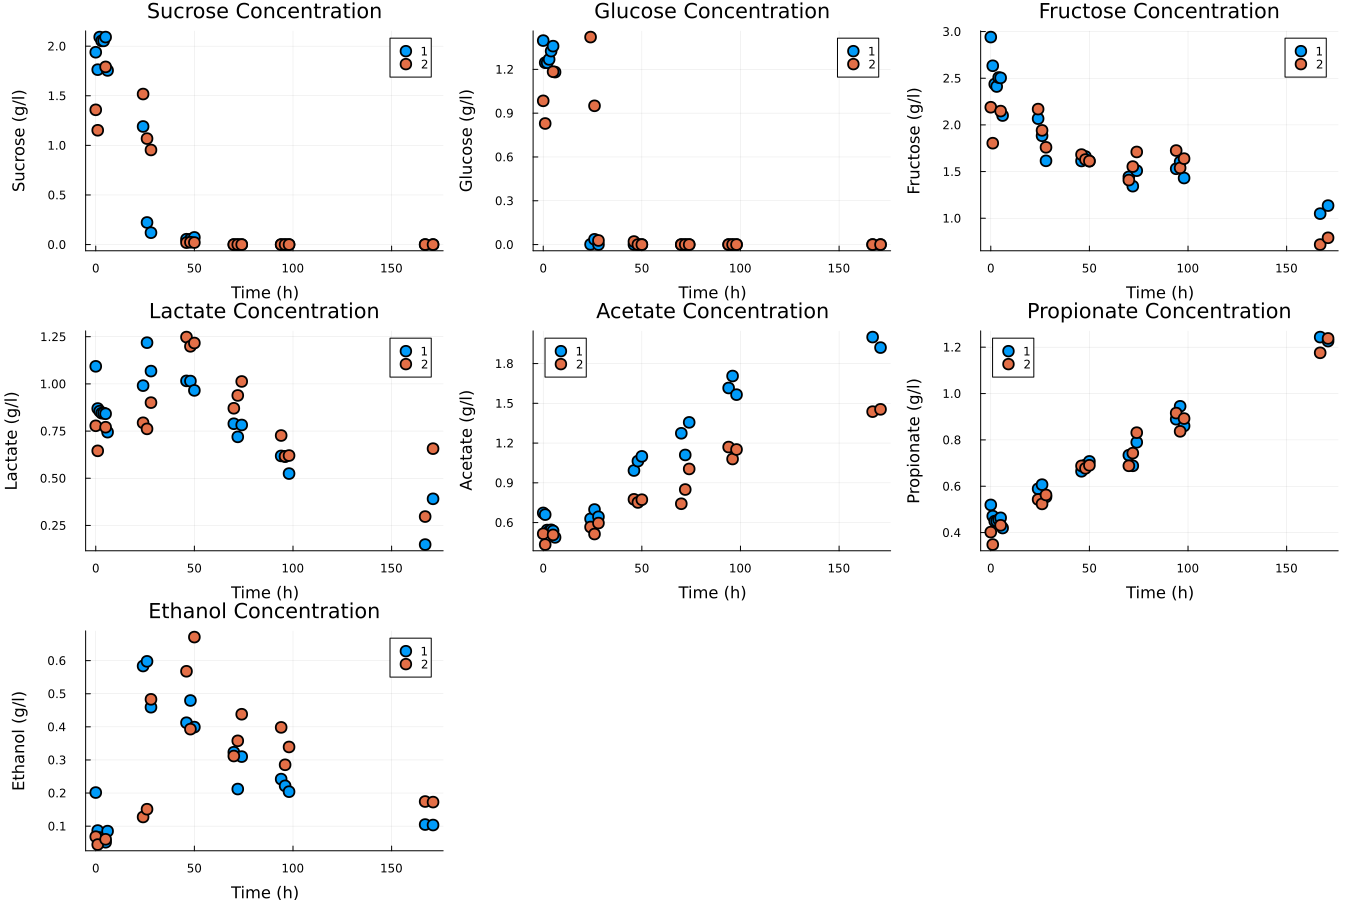
\includegraphics[width=.9\linewidth]{../plots/23_10/final_scatter_23_10.png}
\caption{\label{fig:org19231c4}Συνολικά Αποτελέσματα HPLC - Αρχικό Κινητικό Πείραμα}
\end{figure}

Δύο ακόμη διαγράμματα που θεωρήθηκαν χρήσιμα ήταν τα συγκεντρωτικά διαγράμματα της συγκέντρωσης σακχάρων (\ref{fig:orgabafda4}) και προϊόντων (\ref{fig:org1715b44}), από τα οποία μπορούν να φανούν περισσότερο κάποιες τάσεις που υπάρχουν στην διεργασία.

\begin{figure}[htbp]
\centering
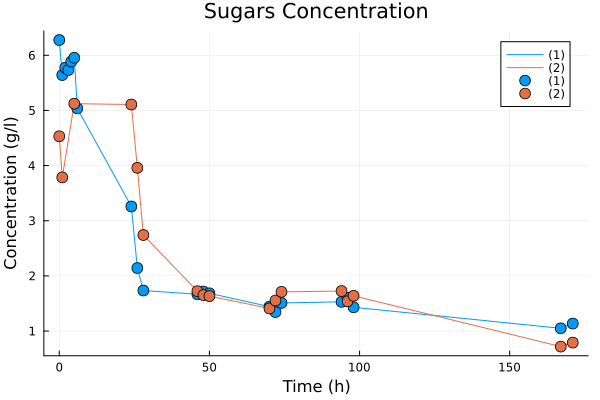
\includegraphics[width=300px]{../plots/23_10/sugars_conc_scatter_23_10.png}
\caption{\label{fig:orgabafda4}Συνολική Συγκέντρωση Σακχάρων - Αρχικό Κινητικό Πείραμα}
\end{figure}

\begin{figure}[htbp]
\centering
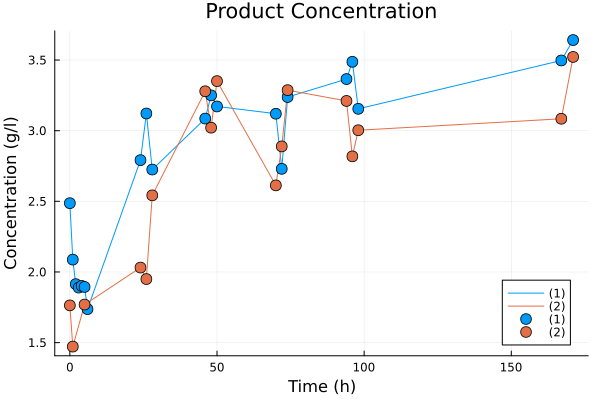
\includegraphics[width=300px]{../plots/23_10/product_conc_scatter_23_10.png}
\caption{\label{fig:org1715b44}Συνολική Συγκέντρωση Προϊόντων - Αρχικό Κινητικό Πείραμα}
\end{figure}

\item Ρυθμός Εξάτμισης Νερού:
\label{sec:org5ada826}
Το τελευταίο δοκιμαστικό πείραμα ήταν για την εξάτμιση του νερού. Ο πίνακας \ref{tab:org79b2af2} δείχνει τα αποτελέσματα της μείωσης της συνολικής υγρής μάζας καθώς και των \acrshort{ts}, από τα οποία προκύπτει η μείωση της μάζας του νερού.

\begin{table}[htbp]
\caption{\label{tab:org79b2af2}Ρυθμός Μεταβολής Υγρής και Ξηρής Μάζας}
\centering
\begin{tabular}{rrrr}
Ημέρα & Μείωση Υγρής Μάζας (g) & Μείωση TS (g) & Εξάτμιση Νερού (g)\\[0pt]
\hline
1 & 6.97 & 1.68 & 5.28\\[0pt]
2 & 12.88 & 2.35 & 10.53\\[0pt]
3 & 15.68 & -0.73 & 16.42\\[0pt]
7 & 36.23 & 5.22 & 31.01\\[0pt]
9 & 38.06 & 3.83 & 34.23\\[0pt]
11 & 44.74 & 5.47 & 39.27\\[0pt]
14 & 45.49 & 7.86 & 37.63\\[0pt]
\end{tabular}
\end{table}

Από τα αποτελέσματα αυτά, παρατηρείται πως η υγρή μάζα αρχικά μειώνεται γρήγορα και μεταξύ 11 και 14 ημερών έχει φτάσει ένα πλατό. Ο ρυθμός εξάτμισης του νερού φαίνεται να έχει παρόμοια τάση, βέβαια την τελευταία ημέρα που έγινε δειγματοληψία, η εξάτμιση μειώθηκε. Τα ευρήματα αυτά οδηγούν στην θεώρηση ότι ο ρυθμός εξάτμισης μπορεί να περιγραφεί πολύ καλά με μία παραβολική εξίσωση. Κάνοντας την προσαρμογή, προκύπτει πως για το πείραμα αυτό, το οποίο διεξάχθηκε στους 35 \(^oC\), ο ρυθμός εξάτμισης δίνεται από την εξίσωση

\[ \text{Evaporation Rate} = -0.252t^2 + 6.287t - 0.723 ~ ~ ~ R^2 = 0.997 \]

με τον χρόνο να είναι εκφρασμένος σε ημέρες.

Για την μείωση των TS δεν μπορεί να προκύψει κάποιο ικανοποιητικό συμπέρασμα, το οποίο συνάδει με τις παρατηρήσεις των άλλων δοκιμαστικών πειραμάτων που έκριναν τα στερεά μη ικανοποιητικά για την παρακολούθηση της υδρόλυσης.
\end{enumerate}

\section{Βασικός πειραματικός κύκλος υδρόλυσης εργαστηριακής κλίμακας}
\label{sec:org0cf19b0}
Για τον βασικό πειραματικό κύκλο της υδρόλυσης, έγιναν 2 πειράματα στα οποία εξετάστηκε η υδρόλυση 5 διαφορετικών αναλογιών \acrshort{mix}/\acrshort{fw}. Οι αναλογίες ήταν 0, 1, 2, 4 και 8 mL \acrshort{mix} ανά 200 g \acrshort{fw}. Η θερμοκρασία ρυθμίστηκε στους 35 \(^oC\) για το πρώτο πείραμα και στους 40 \(^oC\) για το δεύτερο, όπως αναφέρθηκε και στην \autoref{sec:lab-hydro}. Τα πρωτογενή πειραματικά αποτελέσματα ήταν αρχικό και τελικό \acrshort{cod} καθώς και τα αποτελέσματα της HPLC όπως και για το αρχικό κινητικό πείραμα, ενώ τα δευτερογενή συγκριτικά αποτελέσματα μεταξύ των κύκλων θα παρουσιαστούν στο \autoref{sec:result_discussion} στα πλαίσια της συζήτησης των αποτελεσμάτων για να αποφανθούν οι βέλτιστες λειτουργικές συνθήκες.

\begin{enumerate}
\item Πείραμα στους 35 \(^oC\):
\label{sec:orgffed9aa}
Η μεταβολή του \acrshort{cod} κατά τις 72 ώρες ταυτόχρονης υδρόλυσης και ζύμωσης φαίνεται στο Σχήμα \ref{fig:orgf280b23}.

\begin{figure}[htbp]
\centering
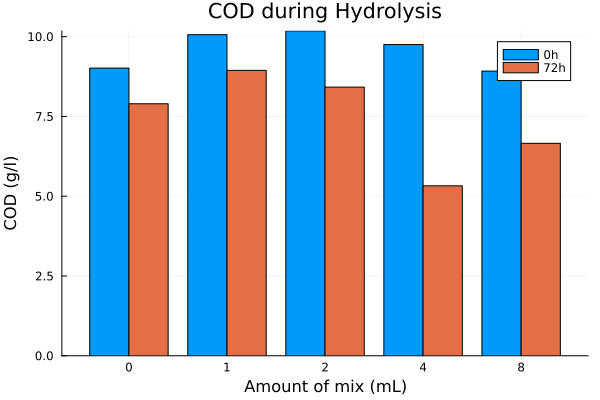
\includegraphics[width=250px]{../plots/10_11/cod_groupedbar_10_11.png}
\caption{\label{fig:orgf280b23}Μεταβολή του COD κατά την υδρόλυση/ζύμωση - Πείραμα 35 \(^oC\)}
\end{figure}

Από την μεταβολή του \acrshort{cod} φαίνεται πως γενικά υπάρχει μία μείωση κατά την διεργασία, το οποίο συμφωνεί και με τα αποτελέσματα των δοκιμαστικών πειραμάτων. Επίσης, φαίνεται πως όσο περισσότερο \acrshort{mix} προστίθεται, η μείωση του \acrshort{cod} γίνεται όλο και περισσότερη. Αυτό εξηγείται, καθώς όσο προστίθεται το \acrshort{mix} προστίθενται ενεργοί μικροοργανισμοί, οι οποίοι όχι μόνο υδρολύουν το υπόστρωμα, αλλά καταναλώνουν και κάποια ποσότητα από το \acrfull{scod}.

Τα συγκεντρωτικά αποτελέσματα της HPLC φαίνονται στο Σχήμα \ref{fig:org588db03}. Εκτός από τα αποτελέσματα αυτά, το διάγραμμα περιέχει και την μέτρηση του pH, η οποία είχε γίνει στο πείραμα αυτό.

\begin{figure}[htbp]
\centering
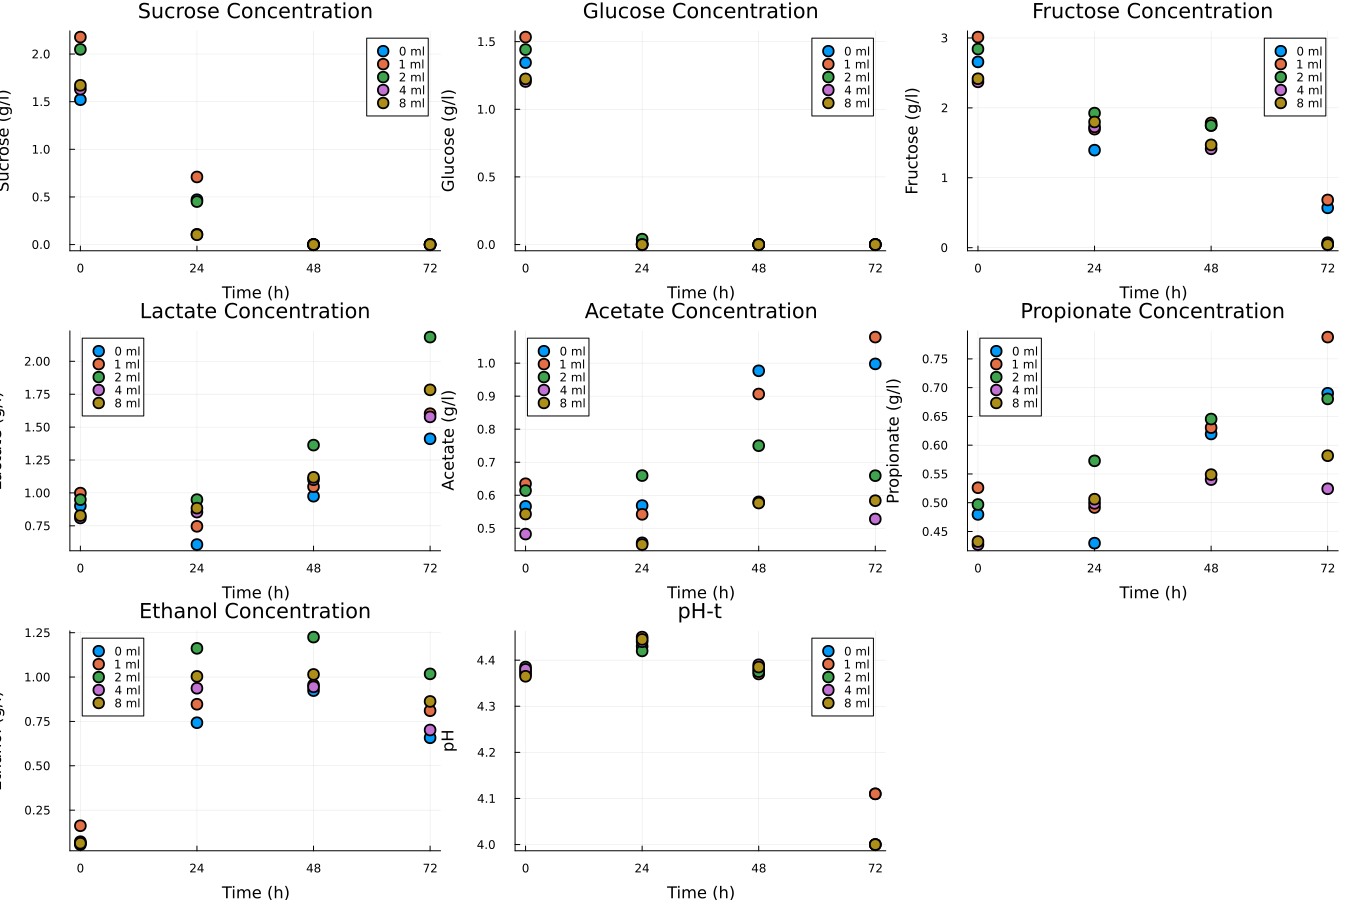
\includegraphics[width=.9\linewidth]{../plots/10_11/final_scatter_10_11.png}
\caption{\label{fig:org588db03}Συνολικά Αποτελέσματα HPLC - Πείραμα 35 \(^oC\)}
\end{figure}

Επίσης παρουσιάζονται τα συγκεντρωτικά διαγράμματα σακχάρων και προϊόντων όπως έγινε και για το αρχικό κινητικό πείραμα. 

\begin{figure}[htbp]
\centering
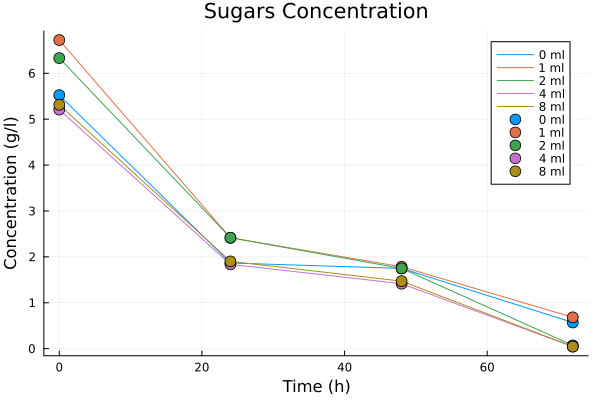
\includegraphics[width=300px]{../plots/10_11/sugars_conc_scatter_10_11.png}
\caption{\label{fig:orga256f31}Συνολική Συγκέντρωση Σακχάρων - Πείραμα 35 \(^oC\)}
\end{figure}

\begin{figure}[htbp]
\centering
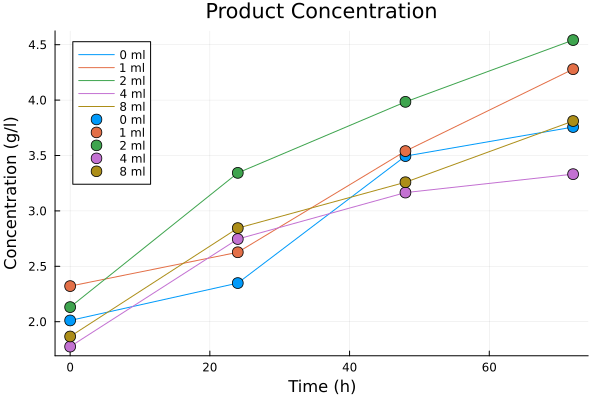
\includegraphics[width=300px]{../plots/10_11/product_conc_scatter_10_11.png}
\caption{\label{fig:orgbb33943}Συνολική Συγκέντρωση Προϊόντων - Πείραμα 35 \(^oC\)}
\end{figure}

\item Πείραμα στους 40 \(^oC\)
\label{sec:orge1fe35a}
Τα αντίστοιχα αποτελέσματα προέκυψαν και από αυτό το πείραμα. Στο Σχήμα \ref{fig:org93939de} φαίνεται η μεταβολή του \acrshort{scod} κατά την διάρκεια της υδρόλυσης/ζύμωσης.

Γ\begin{figure}[htbp]
\centering
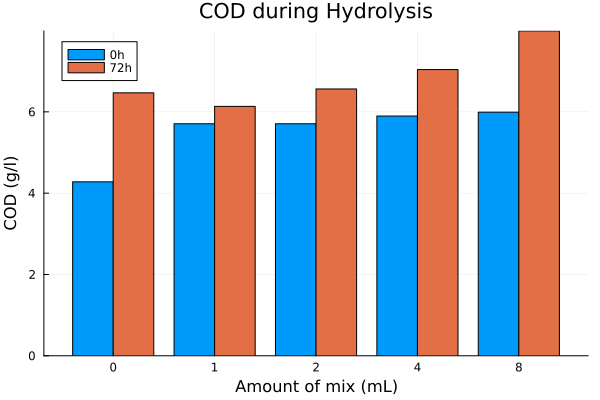
\includegraphics[width=.9\linewidth]{../plots/28_11/cod_groupedbar_28_11.png}
\caption{\label{fig:org93939de}Μεταβολή του COD κατά την υδρόλυση/ζύμωση - Πείραμα 40 \(^oC\)}
\end{figure}

Στο πείραμα αυτό, παρατηρείται μία τάση σχετικά διαφορετική από τα προηγούμενα πειράματα, καθώς το \acrshort{cod} γενικά αυξάνεται με την ζύμωση. Η πιο πιθανή εξήγηση είναι πως το αρχικό \acrshort{cod} ήταν πολύ χαμηλό, οπότε η υδρόλυση είχε γρηγορότερο ρυθμό από την ζύμωση γενικότερα και ως αποτέλεσμα φαίνεται περισσότερο η αύξηση.

Τα αποτελέσματα της HPLC φαίνονται στα Σχήματα \ref{fig:org272f1a5}, \ref{fig:orge86e617} και \ref{fig:orgdf85241}.

\begin{figure}[htbp]
\centering
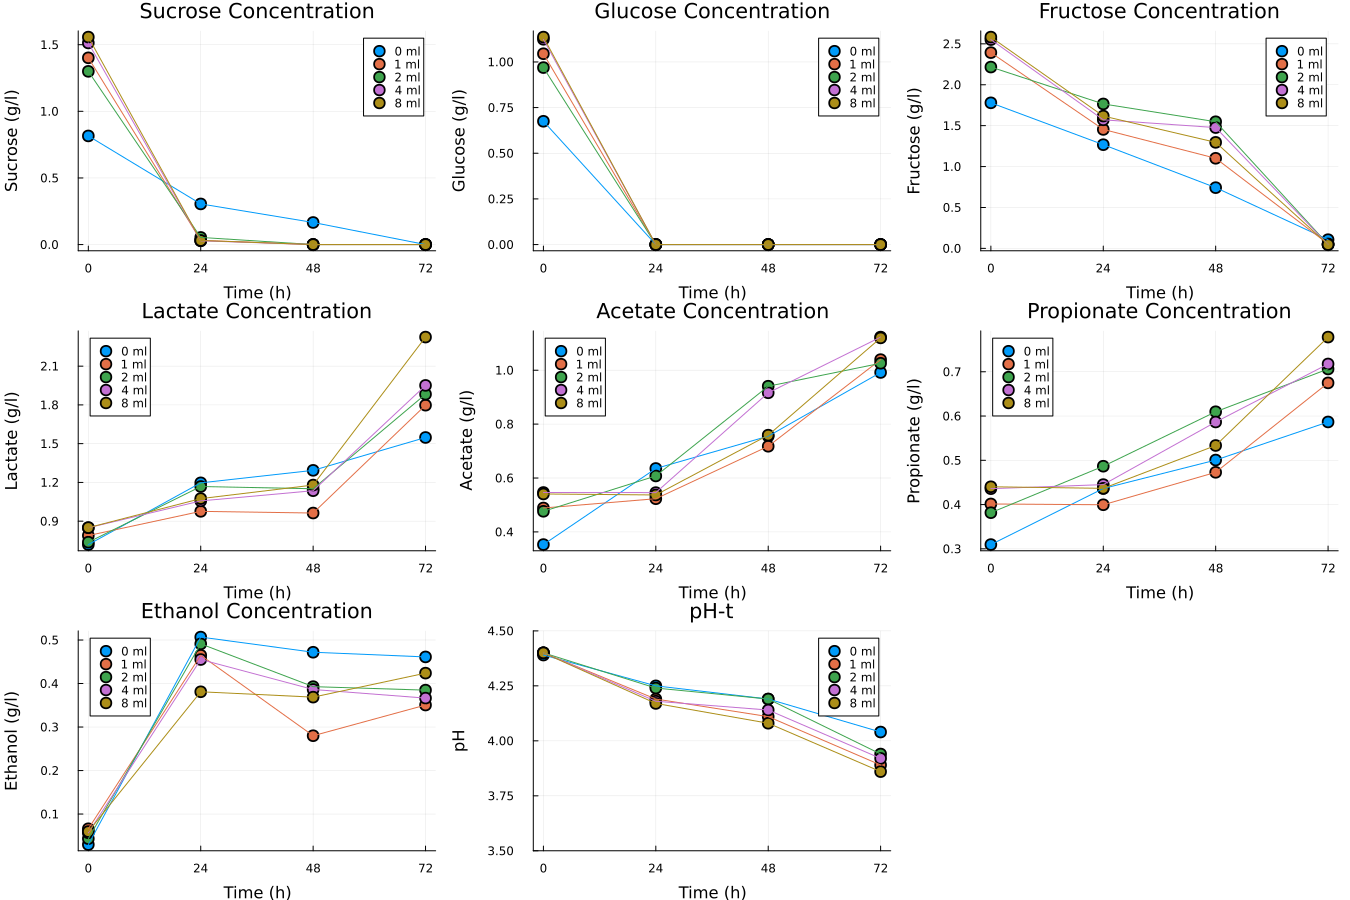
\includegraphics[width=.9\linewidth]{../plots/28_11/final_scatter_28_11.png}
\caption{\label{fig:org272f1a5}Συνολικά Αποτελέσματα HPLC - Πείραμα 40 \(^oC\)}
\end{figure}

\begin{figure}[htbp]
\centering
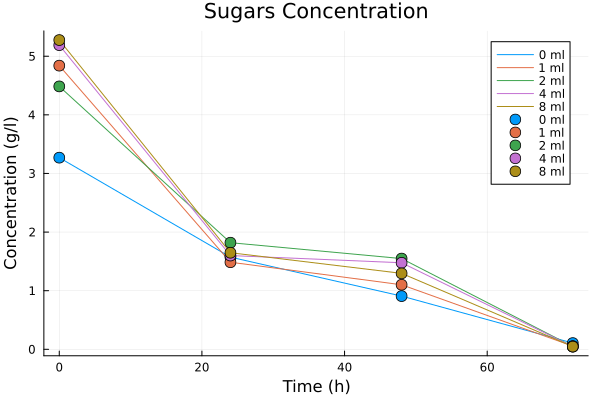
\includegraphics[width=300px]{../plots/28_11/sugars_conc_scatter_28_11.png}
\caption{\label{fig:orge86e617}Συνολική Συγκέντρωση Σακχάρων - Πείραμα 40 \(^oC\)}
\end{figure}

\begin{figure}[htbp]
\centering
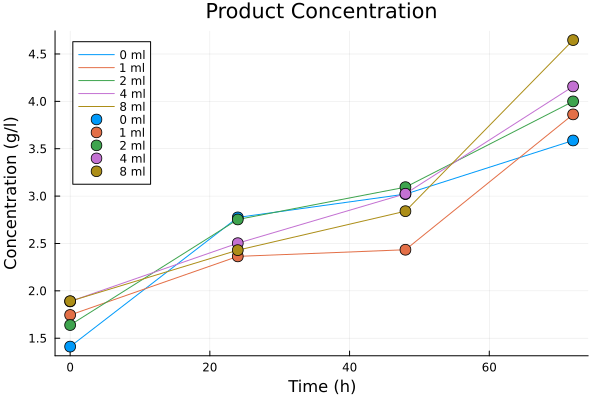
\includegraphics[width=300px]{../plots/28_11/product_conc_scatter_28_11.png}
\caption{\label{fig:orgdf85241}Συνολική Συγκέντρωση Προϊόντων - Πείραμα 40 \(^oC\)}
\end{figure}
\end{enumerate}

\section{Έλεγχος Υποθέσεων και Ανάλυση Ευαισθησίας}
\label{sec:org0b056c2}
Καθώς όμως το προφίλ των παραγόμενων μεταβολικών προϊόντων σε κάθε συνθήκη αποτελεί την βασική απόκριση της διεργασίας, έγιναν και κάποιες πιο λεπτομερείς αναλύσεις. Η βασικότερη είναι μία ανάλυση ευαισθησίας η οποία έδειξε πως μεταβάλλονται τα προϊόντα με την μεταβολή των λειτουργικών συνθηκών. Επίσης όμως έγιναν έλεγχοι υποθέσεων για να εξεταστεί πόσο στατιστικά σημαντική είναι η μεταβολή της κάθε συνθήκης (ποιοτική ανάλυση), ώστε να διαπιστωθεί πως πράγματι έχει νόημα να εξεταστεί η ευαισθησία (ποσοτική ανάλυση). Τέλος, έγινε μία υπολογιστική ανάλυση η οποία προσπάθησε να συνδέσει τα παραγόμενα προϊόντα με τις αντιδράσεις από τις οποίες παράχθηκαν, με σκοπό μία πιο αναλυτική εικόνα των μεταβολικών μονοπατιών που ακολουθήθηκαν. Η ανάλυση αυτή είναι αρκετά ενδιαφέρουσα καθώς μπορεί να δώσει πολλές πληροφορίες για την διεργασία και πως να βελτιστοποιηθεί. Όμως, λόγω της φύσης της ανάλυσης είναι πολύ δύσκολο να επαληθευτεί πειραματικά η εγκυρότητα της. Η ανάλυση αυτή παρουσιάζεται στο Παράρτημα Α.

Για τους ελέγχους υποθέσεων χρησιμοποιήθηκε το πακέτο HypothesisTests.jl μέσω του οποίου μπορούν να γίνουν έλεγχοι όπως το t-test και η \acrfull{anova}. Ένα πρόβλημα που υπάρχει στον έλεγχο αυτόν είναι πως για να επιβεβαιωθεί η στατιστική σημαντικότητα απαιτούνται πολλά δεδομένα και η επανάληψη του κάθε πειράματος πολλές φορές δεν θα ήταν πρακτικά εφικτή. Ένας τρόπος να παραχθούν αρκετά αποτελέσματα για να υπάρχει στατιστική σημαντικότητα χωρίς να γίνουν τόσες επαναλήψεις είναι να υποτεθεί πως τα αποτελέσματα θα ακολουθήσουν κανονική κατανομή. Έτσι, με έναν μέσο όρο και μία τυπική απόκλιση μπορούν να παραχθούν τα απαιτούμενα αποτελέσματα.

Όμως, τα πειράματα που έγιναν είναι λίγα ακόμη και για να προκύψει μία έγκυρη τυπική απόκλιση. Το πείραμα στο οποίο υπάρχουν αρκετά δείγματα για μία έγκυρη τυπική απόκλιση είναι το αρχικό πείραμα. Για καλύτερη ακρίβεια, έγινε η παραδοχή πως όλες οι δειγματοληψίες μέσα σε μία μέρα θα έπρεπε να έχουν την ίδια τιμή (το οποίο στην πράξη δεν ισχύει, αλλά οι αντιδράσεις είναι αργές, οπότε το σφάλμα της παραδοχής αυτής είναι μικρό). Έτσι, προέκυψε μία τυπική απόκλιση για κάθε μέρα του κύκλου αυτού και η απόκλιση που χρησιμοποιήθηκε ήταν ο μέσος όρος αυτών. Παρότι αυτή η διαδικασία δεν είναι τελείως έγκυρη, είναι ο πιο έμπιστος τρόπος να γίνει ένας έλεγχος υποθέσεων με το διαθέσιμο πλήθος δεδομένων.

Έπειτα, έγινε μία δειγματοληψία 20 "πειραμάτων" από τις κατανομές αυτές, οι οποίες ορίστηκαν με την βοήθεια του Distributions.jl \textsuperscript{\citeprocitem{108}{108}}, με τυχαίο τρόπο (με χρήση του πακέτου Random.jl με χρήση του seed 1234 ώστε να υπάρχει τυχαιότητα αλλά τα αποτελέσματα να είναι επαναλήψιμα). Η τιμή 20 επιλέχθηκε ως μία τιμή στην οποία με βάση την στατιστική, ένας έλεγχος υποθέσεων έχει αρκετά καλή ισχύ.

Ο σκοπός της \acrshort{anova} ήταν να εξετάσει αν έχει επίδραση στα προϊόντα η προσθήκη του \acrshort{mix}. Προέκυψε πως και για τις 2 θερμοκρασίες, η προσθήκη του \acrshort{mix} είχε επίδραση σε κάθε προϊόν με στατιστική βεβαιότητα (p-Value < 0.001). Έπειτα, έγινε ένας διαχωρισμός για να διαπιστωθεί αν η προσθήκη παραπάνω από 2 mL \acrshort{mix} έχει επίδραση και αντίστοιχα αν η προσθήκη του \acrshort{mix} έχει επίδραση αν προστεθούν έως 2 mL.

Προέκυψε πως η προσθήκη πάνω από 2 mL έχει επίδραση με στατιστική βεβαιότητα (p-Value < 0.001). Στους 35 \(^oC\), η επίδραση αυτή είναι αρνητική, ενώ στους 40 \(^oC\) είναι θετική. Για τους 40 \(^oC\), εξετάστηκε αν έχει κάποια επίδραση η προσθήκη 8 mL \acrshort{mix} σε σχέση με τα 4. Από τον έλεγχο αυτόν, προέκυψε πως το οξικό δεν επηρεάζεται από την προσθήκη αυτή (p-Value = 0.9) ενώ δεν υπάρχουν αρκετά δεδομένα για να απορριφθεί η υπόθεση πως η αιθανόλη δεν μεταβάλλεται (p-Value = 0.03). 

Για τις ποσότητες από 2 mL και κάτω, προέκυψε πως στους 35 \(^oC\) η προσθήκη επηρεάζει την ποσότητα κάθε προϊόντος με στατιστική σημαντικότητα (p-Value < 0.001). Το γαλακτικό οξύ και η αιθανόλη επηρεάζονται θετικά ενώ το οξικό οξύ και το προπιονικό οξύ αρνητικά. Στους 40 \(^oC\), μόνο το γαλακτικό και το προπιονικό οξύ επηρεάζονται με στατιστικά σημαντικό τρόπο (p-Value < 0.001) ενώ για το οξικό οξύ και την αιθανόλη δεν μπορεί να προκύψει ασφαλώς το συμπέρασμα αυτό (με p-Value = 0.14 και 0.06 αντίστοιχα).

Τέλος, έγινε ένα t-test για να εξεταστεί ποια προϊόντα επηρεάζονται από την θερμοκρασία. Διαπιστώθηκε πως η θερμοκρασία επηρέασε την παραγωγή κάθε προϊόντος σε κάθε θερμοκρασία (p-Value < 0.001) με μοναδική εξαίρεση το οξικό οξύ σε ποσότητες 0 και 1 mL \acrshort{mix}, το οποίο ήταν ίδιο σε κάθε θερμοκρασία (p-Value = 0.92 και 0.46 αντίστοιχα).

Έχοντας επιβεβαιώσει ποιες μεταβολές έχουν στατιστική σημαντικότητα, έγινε μία ανάλυση ευαισθησίας για να ποσοτικοποιηθούν τα παραπάνω αποτελέσματα. Η ανάλυση ευαισθησίας έγινε με το πακέτο GlobalSensitivity.jl \textsuperscript{\citeprocitem{109}{109}} και συγκεκριμένα με την μέθοδο Morris. Ένα πρόβλημα στην εφαρμογή της ανάλυσης ευαισθησίας είναι πως δεν μπορεί να λειτουργήσει με διακριτά σημεία, αλλά χρειάζεται μία συνεχή συνάρτηση. Έγινε η παραδοχή πως από το ένα πειραματικό σημείο στο άλλο η συσχέτιση είναι γραμμική και άρα μπορεί να γίνει μία γραμμική παρεμβολή για να προκύψει η συνάρτηση. Αυτό δεν είναι σίγουρα σωστό, αλλά δεν μπορεί να διαπιστωθεί η ύπαρξη κάποιας μη γραμμικότητας χωρίς να διεξαχθούν περισσότερα πειράματα. Η παρεμβολή έγινε με το πακέτο Interpolations.jl \textsuperscript{\citeprocitem{110}{110}} το οποίο έχει την δυνατότητα παρεμβολής στα δεδομένα 2 διαστάσεων (θερμοκρασίας και ποσότητας \acrshort{mix}) που έχουν προκύψει. Η ανάλυση ευαισθησίας έγινε ολικά αλλά και στις 3 υποπεριοχές που έγιναν και οι έλεγχοι υποθέσεων (0-2 mL \acrshort{mix}, 2-8 mL \acrshort{mix} και ξεχωριστά ανά θερμοκρασία) και τα αποτελέσματα τους παρουσιάζονται παρακάτω με χρήση διαγραμμάτων τυφώνα (tornado diagram), το οποίο συνηθίζεται για αποτελέσματα ευαισθησίας. Στο Σχήμα \ref{fig:org5fc1157} φαίνεται η ολική ανάλυση ευαισθησίας.

\begin{figure}[htbp]
\centering
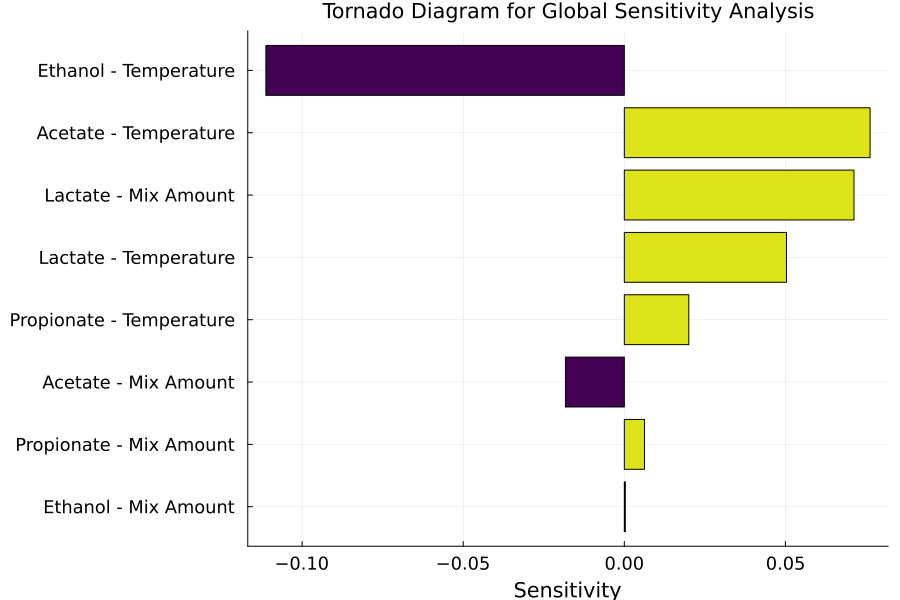
\includegraphics[width=300px]{../plots/sensitivity/global_tornado.png}
\caption{\label{fig:org5fc1157}Ολική Ανάλυση Ευαισθησίας}
\end{figure}

Το οξικό οξύ φαίνεται να έχει αρνητική επίδραση στην ποσότητα του \acrshort{mix}, το οποίο δείχνει πως αν η προ-επεξεργασία έχει σκοπό την προετοιμασία ενός υδρολύματος για αναερόβια χώνευση, η προσθήκη του \acrshort{mix} είναι επιβλαβής. Όμως, αν εξεταστούν ξεχωριστά οι 2 θερμοκρασίες, όπως στο Σχήμα \ref{fig:orgdb103e7}, θα διαπιστωθεί πως αυτό ισχύει μόνο στους 35 \(^oC\), όπου οι μικροοργανισμοί που παράγουν αιθανόλη επικρατούν και καταναλώνουν το υπόστρωμα που θα γινόταν οξικό, ενώ στους 40 \(^oC\) που αυτοί έχουν απενεργοποιηθεί, το οξικό παράγεται σε μεγαλύτερη ποσότητα. Η αλληλεπίδραση αυτή θεωρήθηκε καθώς η αιθανόλη και το οξικό οξύ αποτελούν τα δύο προϊόντα που προέρχονται από το Acetyl-CoA και ενισχύθηκε από τα συμπεράσματα της ανάλυσης που φαίνεται στο Παράρτημα A. 

\begin{figure}[htbp]
\centering
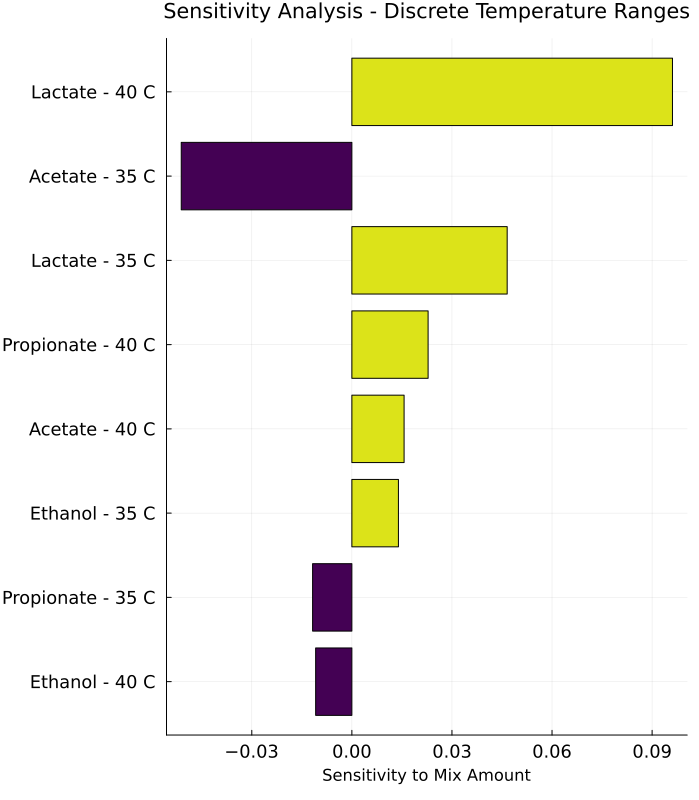
\includegraphics[width=300px]{../plots/sensitivity/temperature_tornado.png}
\caption{\label{fig:orgdb103e7}Ανάλυση ευαισθησίας σε διακριτές θερμοκρασίες}
\end{figure}

Άλλο ένα συμπέρασμα το οποίο προκύπτει από το Σχήμα \ref{fig:org5fc1157} το οποίο δεν είναι ακριβώς σωστό είναι η επίδραση της ποσότητας του \acrshort{mix} στην αιθανόλη. Στην περιοχή 0-2 mL \acrshort{mix}, έχει μία μεγάλη θετική επίδραση, ενώ αν η ποσότητα \acrshort{mix} αυξηθεί περαιτέρω, παράγεται όλο και λιγότερη αιθανόλη, με αποτέλεσμα αυτές να αλληλοαναιρούνται και να φαίνεται μία μηδενική επίδραση στο σύνολο. Για τον σκοπό αυτόν, αλλά και την διαπίστωση αν το πρόβλημα αυτό παρουσιάζεται σε κάποια άλλη ένωση, έγιναν οι αναλύσεις ευαισθησίας για τις 2 αυτές υποπεριοχές, οι οποίες φαίνονται στα Σχήματα \ref{fig:org2c771fe} και \ref{fig:org99640c0}.

\begin{figure}[htbp]
\centering
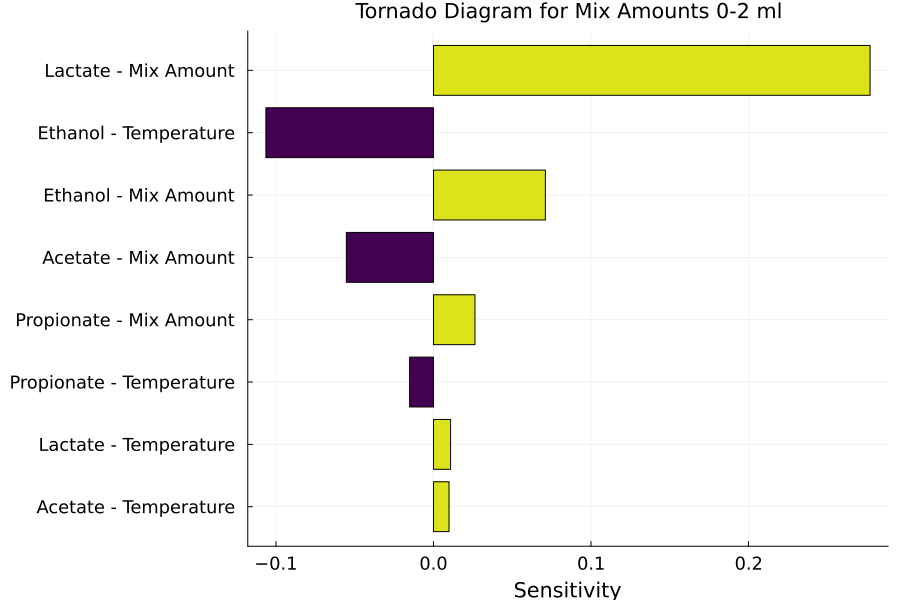
\includegraphics[width=300px]{../plots/sensitivity/tornado_low.png}
\caption{\label{fig:org2c771fe}Ανάλυση Ευαισθησίας στην περιοχή 0-2 mL μιξ}
\end{figure}

Από το Σχήμα \ref{fig:org2c771fe} φαίνεται η θετική αυτή επίδραση της αιθανόλης στην ποσότητα \acrshort{mix}, μία ακόμη σημαντικότερη επίδραση της ποσότητας αυτής στο γαλακτικό και πως οι επιδράσεις της θερμοκρασίας είναι ακρετά μικρές, το οποίο δείχνει πως σε αυτές τις ποσότητες δεν είναι τόσο σημαντική η επίδραση της θερμοκρασίας.

\begin{figure}[htbp]
\centering
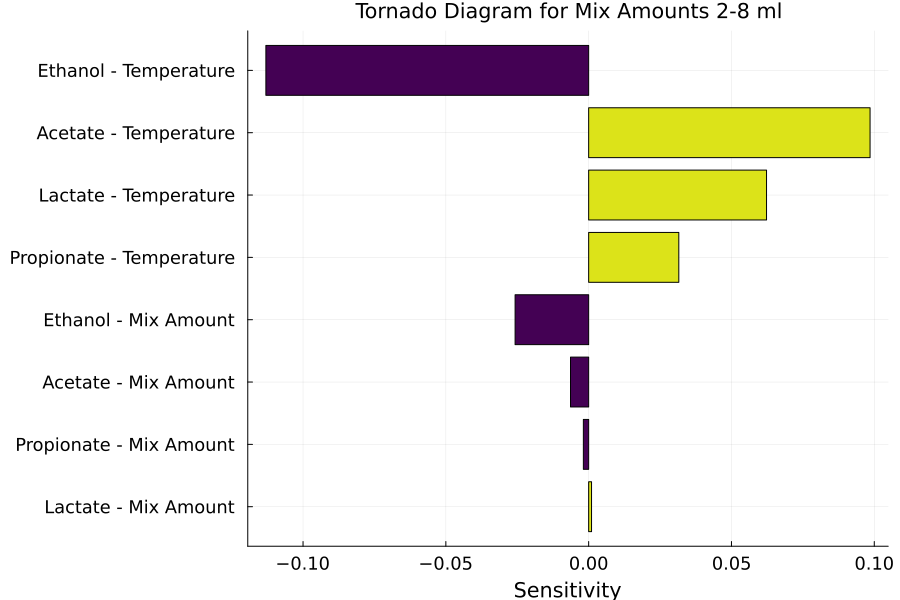
\includegraphics[width=300px]{../plots/sensitivity/tornado_high.png}
\caption{\label{fig:org99640c0}Ανάλυση Ευαισθησίας στην περιοχή 2-8 mL μιξ}
\end{figure}

Στο Σχήμα \ref{fig:org99640c0} φαίνεται πως η αιθανόλη έχει μία σημαντική αρνητική επίδραση στην ποσότητα του \acrshort{mix} και ότι οι άλλες 3 ενώσεις έχουν αμελητέα επίδραση, το οποίο ενισχύει την υπόθεση ότι γενικά δεν έχει ιδιαίτερα μεγάλη επίδραση η προσθήκη παραπάνω από 2 mL.

\section{Πειράματα υδρόλυσης πιλοτικής κλίμακας}
\label{sec:orgffc888f}
Στην πιλοτική κλίμακα έγιναν 3 πειράματα υδρόλυσης, οι συνθήκες των οποίων φαίνονται στην \autoref{sec:pilot-exp} . Παρακάτω, φαίνονται τα στερεά και το \acrshort{cod} για το κάθε πείραμα. Αξίζει να σημειωθεί πως η καθημερινή τροφοδοσία στο όργανο αυτό δεν είναι ίδια, καθώς τα υπολείμματα τροφών που συλλέγονται από ένα εστιατόριο έχουν εκ φύσεων ανομοιογένεια από μέρα σε μέρα. Οπότε, μπορούν να παρατηρηθούν αποκλίσεις που οφείλονται σε αυτό στα παρακάτω αποτελέσματα. Για τον λόγο αυτόν, ως υπόστρωμα στην αναερόβια χώνευση χρησιμοποιήθηκε μία υγρή απορροή που αποτελείται από μίγμα των απορροών των 4 ημερών και περιγράφεται από τον μέσο όρο και την τυπική απόκλιση που φαίνονται σε κάθε πίνακα. Η τυπική απόκλιση αυτή είναι και ένα μέτρο του πόσο σφάλμα αναμένεται να υπάρχει λόγω της ανομοιογένειας στην τροφοδοσία.

\begin{table}[htbp]
\caption{\label{tab:org8683560}Υδρόλυση Πιλοτικής Κλίμακας - Πρώτος Κύκλος}
\centering
\begin{tabular}{rrrrrrr}
Day & TS (\(\%\)) & VS (\(\%\)) & VS/TS (\(\%\)) & sCOD (mg/L) & tCOD (mg/L) & sCOD/tCOD (\(\%\))\\[0pt]
\hline
1 & 0.63 & 0.54 & 86.08 & 4561.5 & 8792.7 & 51.88\\[0pt]
2 & 1.26 & 1.17 & 92.64 & 8135.1 & 13077.5 & 62.21\\[0pt]
3 & 2.54 & 2.48 & 97.38 & 11134.4 & 37476.6 & 29.71\\[0pt]
4 & 2.47 & 2.42 & 97.79 & 12991.1 & 32053.8 & 40.53\\[0pt]
 &  &  &  &  &  & \\[0pt]
Mean & 1.73 & 1.65 & 93.47 & 9205.5 & 22850.2 & 46.08\\[0pt]
StDev & 0.81 & 0.83 & 4.73 & 3192.3 & 12163.0 & 12.17\\[0pt]
\end{tabular}
\end{table}

\begin{table}[htbp]
\caption{\label{tab:org94999ed}Υδρόλυση Πιλοτικής Κλίμακας - Δεύτερος Κύκλος}
\centering
\begin{tabular}{rrrrrrr}
Day & TS (\(\%\)) & VS (\(\%\)) & VS/TS (\(\%\)) & sCOD (mg/L) & tCOD (mg/L) & sCOD/tCOD (\(\%\))\\[0pt]
\hline
1 & 1.07 & 0.97 & 91.05 & 6659.2 & 14029.6 & 47.47\\[0pt]
2 & 0.62 & 0.51 & 82.13 & 4754.9 & 9387.8 & 50.65\\[0pt]
3 & 0.59 & 0.50 & 85.67 & 3088.6 & 9149.8 & 33.76\\[0pt]
4 & 1.54 & 1.48 & 96.28 & 5421.4 & 21699.1 & 24.98\\[0pt]
 &  &  &  &  &  & \\[0pt]
Mean & 0.95 & 0.87 & 88.78 & 4981.0 & 13566.6 & 39.21\\[0pt]
StDev & 0.39 & 0.40 & 0.40 & 1288.7 & 5082.4 & 10.38\\[0pt]
\end{tabular}
\end{table}

\begin{table}[htbp]
\caption{\label{tab:org6a2312d}Υδρόλυση Πιλοτικής Κλίμακας - Τρίτος Κύκλος}
\centering
\begin{tabular}{rrrrrrr}
Day & TS (\(\%\)) & VS (\(\%\)) & VS/TS (\(\%\)) & sCOD (mg/L) & tCOD (mg/L) & sCOD/tCOD (\(\%\))\\[0pt]
\hline
1 & 1.10 & 1.05 & 95.01 & 6326.0 & 13791.6 & 45.87\\[0pt]
2 & 0.65 & 0.59 & 91.55 & 2326.9 & 7781.1 & 29.90\\[0pt]
3 & 0.57 & 0.52 & 89.81 & 1184.3 & 6650.4 & 17.81\\[0pt]
4 & 1.00 & 0.92 & 92.29 & 4600.2 & 12333.8 & 37.30\\[0pt]
 &  &  &  &  &  & \\[0pt]
Mean & 0.83 & 0.77 & 92.16 & 3609.3 & 10139.2 & 32.72\\[0pt]
StDev & 0.22 & 0.22 & 1.87 & 1993.0 & 2995.4 & 10.30\\[0pt]
\end{tabular}
\end{table}

\section{Πειράματα αναερόβιας χώνευσης}
\label{sec:org65bc79b}
\begin{enumerate}
\item Προετοιμασία υποστρώματος για αναερόβια χώνευση:
\label{sec:org24c4523}
Για να προετοιμαστεί υπόστρωμα για την αναερόβια χώνευση έγινε μία επανάληψη του πειράματος υδρόλυσης εργαστηριακής κλίμακας στους 40 \(^oC\), καθώς τα υδρολύματα δεν είχαν αποθηκευτεί. Σε αυτά έγινε μέτρηση μόνο του \acrshort{cod}, αλλά αναλύθηκε και το \acrfull{tcod} για να εξεταστεί η βιοαποδομησιμότητα που δεν έγινε στα προηγούμενα πειράματα. Το διάγραμμα αυτό φαίνεται στο Σχήμα \ref{fig:orgf4bf913}.

\begin{figure}[htbp]
\centering
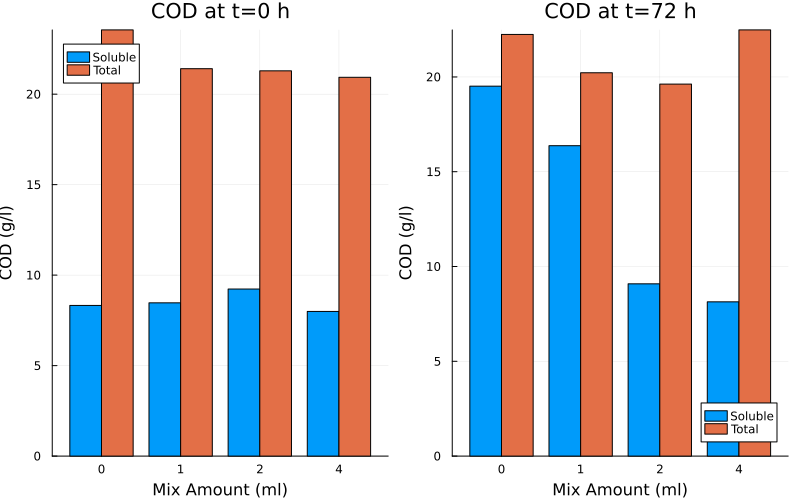
\includegraphics[width=300px]{../plots/26_03/complete_cod_bar_26_03.png}
\caption{\label{fig:orgf4bf913}COD Υδρολυμάτων για προετοιμασία Αναερόβιας Χώνευσης}
\end{figure}

Το ολικό \acrshort{cod} έμεινε περίπου σταθερό, ενώ το διαλυτό αυξήθηκε στις περισσότερες περιπτώσεις. Η μεγάλη αύξηση στις ποσότητες 0 και 1 mL οφείλεται στο γεγονός ότι έγινε υδρόλυση, αλλά υπήρχαν λιγότεροι μικροοργανισμοί για να καταναλώσουν τα υδρολύματα.

\item Μεθοδολογία επεξεργασίας αποτελεσμάτων:
\label{sec:org13fc466}
Εφόσον προετοιμάστηκαν αυτά, άρχισε ο πρώτος πειραματικός κύκλος \acrshort{ad}. Η ανάλυση των αποτελεσμάτων ήταν αντίστοιχη για κάθε ένα από τα πειράματα. Από τα πειράματα, συλλεγόντουσαν φωτογραφίες με τις στάθμες των προχοΐδων, από τις οποίες υπολογιζόταν ο παραγόμενος όγκος μεθανίου. Καθώς οι φωτογραφίες είχαν timestamps, ήταν εύκολο να υπολογιστεί η χρονική στιγμή κάθε φωτογραφίας, γνωρίζοντας ποιά είναι η στιγμή 0. Για την αυτοματοποίηση της ανάλυσης αυτής χρησιμοποιήθηκε η βιβλιοθήκη Dates.jl η οποία είναι built-in στην Julia \textsuperscript{\citeprocitem{102}{102}} . Η βιβλιοθήκη αυτή αποθηκεύει την κάθε χρονική στιγμή, με βάση την τελευταία χρονική υποδιαίρεση που έχει (στην περίπτωση αυτή msec). Οπότε, έγινε μετατροπή αυτού σε πιο χρήσιμες μονάδες χρόνου όπως τα λεπτά και οι ώρες. Για τον παραγόμενο όγκο μεθανίου σε κάθε περίπτωση, είναι πιο χρήσιμος ο αθροιστικός όγκος και όχι ο στιγμιαίος, ο οποίος μπορεί να υπολογιστεί εύκολα με την συνάρτηση \texttt{cumsum}.

Έπειτα, έγινε μία προσαρμογή των δεδομένων του όγκου μεθανίου με τον χρόνο, χρησιμοποιώντας το τροποποιημένο μοντέλο Gompertz, όπως αναφέρθηκε στην \autoref{sec:gompertz}. Αυτή έγινε με την βοήθεια της βιβλιοθήκης LsqFit.jl, η οποία χρησιμοποιεί τον αλγόριθμο Levenberg-Marquardt, όπως αυτός έχει γραφθεί στην βιβλιοθήκη Optim.jl \textsuperscript{\citeprocitem{111}{111}} για την προσαρμογή σε μη γραμμικά μοντέλα. Εκτός από αυτήν την προσαρμογή, έγινε και μία προσαρμογή στα δεδομένα όγκου μεθανίου ανά g VS λάσπης στον αντιδραστήρα. Αυτό είναι σημαντικό καθώς ο ρυθμός παραγωγής μεθανίου ανά g VS λάσπης αποτελεί την \acrfull{sma}, η οποία είναι ιδιαίτερα σημαντική για την σύγκριση των αποτελεσμάτων. Για κάθε μοντέλο υπολογίστηκε ο συντελεστής προσαρμογής R\textsuperscript{2}, για να διαπιστωθεί αν έγινε καλά η προσαρμογή.

Παρακάτω θα παρουσιαστούν κάποια διαγράμματα για την παραγωγή μεθανίου από κάθε υδρόλυμα σε κάθε κύκλο, καθώς και πίνακες με τις σταθερές του κάθε μοντέλου που προσαρμόστηκε.

\item ΑΧ εργαστηριακών υδρολυμάτων με Λάσπη 1:
\label{sec:org305ee87}
Για τον κύκλο αυτόν, αρχικά εξετάστηκε η παραγωγή μεθανίου από οξικό οξύ. Βρέθηκε, πως το οξικό οξύ μπορεί να παράγει \(34.2 \pm 12.0 \text{ mL CH$_4$}\). Θεωρητικά, 1 g \acrshort{cod}-eq οξικού οξέος πρέπει να παράγει 350 mL μεθάνιο. Οπότε, αυτά τα πειραματικά αποτελέσματα είναι αρκετά λογικά. Η \acrshort{sma} σε αυτό το πείραμα ήταν \(261.48 \pm 74.36 \frac{\text{mL CH4}}{\text{gVS hour}}\).

Όταν οι αντιδραστήρες τροφοδοτήθηκαν με υδρολύματα, προέκυψαν τα αποτελέσματα του Σχήματος \ref{fig:orgc17c4db} και του Πίνακα \ref{tab:orgdc5f198}.

\begin{figure}[htbp]
\centering
\includesvg[width=.9\linewidth]{../plots/BMPs/methane_s1_r1_comp}
\caption{\label{fig:orgc17c4db}Παραγωγή Μεθανίου από Εργαστηριακά Υδρολύματα - Λάσπη 1}
\end{figure}

\begin{table}[htbp]
\caption{\label{tab:orgdc5f198}Κινητικές Σταθερές Παραγωγής Μεθανίου για Εργαστηριακά Υδρολύματα με Λάσπη 1}
\centering
\begin{tabular}{lrrrr}
Reactor & BMP (mL) & SMA (mL/gVS hour) & Lag Time (hour) & R\textsubscript{squared}\\[0pt]
\hline
Hydro 0 & 5.56 & 0.061 & 5.994 & 0.992\\[0pt]
Hydro 1 & 11.309 & 0.17 & 3.652 & 0.979\\[0pt]
Hydro 2 & 7.182 & 0.121 & 1.108 & 0.991\\[0pt]
Hydro 4 & 5.902 & 0.11 & 1.948 & 0.988\\[0pt]
FW & 2.09 & 0.064 & 1.174 & 0.984\\[0pt]
\end{tabular}
\end{table}

Η παραγωγή μεθανίου στα πειράματα αυτά ήταν αρκετά χαμηλή σε σχέση με αυτήν του οξικού. Για να διαπιστωθεί αν μπορεί να επαναληφθεί το αποτέλεσμα αυτό (για να κριθεί και η εγκυρότητα του), έγινε μία 2η τροφοδοσία στον κύκλο αυτόν. Τα αποτελέσματα του κύκλου αυτού φαίνονται στο Σχήμα \ref{fig:org7e013c5} και στον Πίνακα \ref{tab:org1a9569e}.

\begin{figure}[htbp]
\centering
\includesvg[width=.9\linewidth]{../plots/BMPs/methane_s1_r2_comp}
\caption{\label{fig:org7e013c5}Παραγωγή Μεθανίου από Υδρολύματα - Λάσπη 1 (Επανάληψη)}
\end{figure}

\begin{table}[htbp]
\caption{\label{tab:org1a9569e}Κινητικές Σταθερές Παραγωγής Μεθανίου για Υδρολύματα με Λάσπη 1 (Επανάληψη)}
\centering
\begin{tabular}{lrrrr}
Reactor & BMP (mL) & SMA (mL/gVS hour) & Lag Time (hour) & R\textsubscript{squared}\\[0pt]
\hline
Hydro 0 & 3.726 & 0.028 & 3.854 & 0.992\\[0pt]
Hydro 1 & 10.568 & 0.071 & 4.425 & 0.996\\[0pt]
Hydro 2 & 7.774 & 0.074 & 0.0 & 0.923\\[0pt]
Hydro 4 & 8.294 & 0.052 & 0.348 & 0.988\\[0pt]
FW & 2.593 & 0.04 & 2.666 & 0.988\\[0pt]
\end{tabular}
\end{table}

Στον κύκλο αυτόν, φαίνεται γενικά μία καλή επαναληψιμότητα. Εμφανίζονται οι ίδιες τάσεις στην ποσότητα μεθανίου που παράγεται και παρόμοιοι χρόνοι καθυστέρησης. Οι \acrshort{sma} είναι χαμηλότερες, το οποίο εξηγείται καθώς το προηγούμενο πείραμα έγινε ακριβώς μετά την τροφοδοσία με οξικό οξύ, όπου η λάσπη πιο ενεργή. Η βασική διαφορά αυτού του πειράματος ήταν το πείραμα με το υδρόλυμα με 2 mL \acrshort{mix} το οποίο είχε μηδενικό χρόνο καθυστέρησης επειδή είχε γρήγορη παραγωγή μεθανίου στη φάση αυτή.

Όμως, αυτό που έμεινε περίπου ίδιο στις δύο επαναλήψεις ήταν ότι η παραγωγικότητα ήταν σχετικά χαμηλή. Αρχικά, μετρήθηκε το τελικό pH στον κάθε αντιδραστήρα για να εξεταστεί αν αυτό έπαιξε ρόλο στην χαμηλή παραγωγικότητα. Τα αποτελέσματα φαίνονται στον Πίνακα \ref{tab:org358d3d6}.

\begin{table}[htbp]
\caption{\label{tab:org358d3d6}Τελικό pH Αντιδραστήρων Αναερόβιας Χώνευσης με Λάσπη 1}
\centering
\begin{tabular}{rr}
Αριθμός & pH\\[0pt]
\hline
0 & 8.93\\[0pt]
1 & 7.76\\[0pt]
2 & 7.19\\[0pt]
4 & 6.76\\[0pt]
FW & 4.22\\[0pt]
\end{tabular}
\end{table}

Οι αντιδραστήρες με ανεπεξέργαστο \acrshort{fw} και υδρόλυμα χωρίς προσθήκη \acrshort{mix} είχαν ακραία pH τα οποία μπορεί να επηρέασαν την διεργασία, αλλά στα άλλα 3, το pH δεν ήταν το πρόβλημα.

Σε μία προσπάθεια να βρεθεί το πρόβλημα που οδήγησε στην χαμηλή σχετικά παραγωγικότητα, έγινε ένας δεύτερος κύκλος, χρησιμοποιώντας λάσπη διαφορετικής ενεργότητας και σε διπλάσια ποσότητα, όπως περιγράφηκε και στην \autoref{sec:exp-ad}.

\item ΑΧ εργαστηριακών υδρολυμάτων με Λάσπη 2:
\label{sec:orgf88bdb6}
Για τον κύκλο αυτόν, έγινε πάλι μία δοκιμή με οξικό οξύ με σκοπό την μέτρηση του μέγιστου ρυθμού παραγωγής μεθανίου. Με την προσθήκη του οξικού, παράχθηκε μία ποσότητα μεθανίου, η οποία ήταν της τάξης του \(11.0 \pm 2.9 \text{ mL CH$_4$}\) μέσα στα πρώτα 10-15 λεπτά. H \acrshort{sma} στο διάστημα αυτό ήταν \(68.54 \pm 32.36 \frac{\text{mL CH$_4$}}{\text{gVS hour}}\). Οπότε, φαίνεται πως η λάσπη αυτή είναι λιγότερο δραστική από την προηγούμενη.

Όμως, στο πείραμα αυτό, υπήρξε μία ιδιορρυθμία. Μετά την ταχεία παραγωγή αυτή, δεν παράχθηκε μεθάνιο για μερικές ώρες και μετά από 10 ξανά ξεκίνησε σε έναν αντιδραστήρα η παραγωγή μεθανίου με αργότερο ρυθμό (και μέσα σε 24 ώρες είχαν ξανά ξεκινήσει την παραγωγή όλοι οι αντιδραστήρες). Αυτή η παραγωγή αφέθηκε για 90 ώρες περίπου και βρέθηκε να είναι της τάξης των \(84.6 \pm 18.1 \text{ mL CH$_4$}\) και είχε \acrshort{sma} \(13.51 \pm 4.04 \frac{\text{mL CH$_4$}}{\text{gVS hour}}\).

Οπότε, θεωρήθηκε πως η λάσπη είχε αποθηκευμένη κάποια άλλη τροφή, από την οποία παράχθηκε το μεθάνιο αυτό. Όμως, μέσα στην παραγωγή αυτή είναι πιθανόν να ήταν και κάποια ποσότητα μεθανίου που παράχθηκε από οξικό, μιας και η παραγωγή που έγινε στην αρχή του πειράματος ήταν πολύ χαμηλή.

Κατά την τροφοδοσία με τα υδρολύματα, παρατηρήθηκε πάλι πολύ μεγάλη παραγωγή μεθανίου. Όμως, όταν αφαιρέθηκε η ποσότητα μεθανίου η οποία είχε παραχθεί στην αργή φάση από το οξικό (η οποία οφειλόταν μάλλον σε άλλη τροφή), παρατηρήθηκε πως τα αποτελέσματα έβγαιναν αρκετά λογικά. Οπότε, τα αποτελέσματα που παρουσιάζονται είναι η παραγωγή μεθανίου από τα υδρολύματα, αφαιρόντας την παραγωγή εκείνης της φάσης, θεωρώντας ότι οφείλεται σε κάτι άλλο, το οποίο δεν μπορούμε να ελέγξουμε. Τα διορθωμένα αυτά αποτελέσματα παρουσιάζονται στο Σχήμα \ref{fig:orgf60542a} και στον Πίνακα \ref{tab:orga84f669}.

\begin{figure}[htbp]
\centering
\includesvg[width=.9\linewidth]{../plots/BMPs/methane_s2_r1_comp}
\caption{\label{fig:orgf60542a}Παραγωγή Μεθανίου από Εργαστηριακά Υδρολύματα - Λάσπη 2}
\end{figure}

\begin{table}[htbp]
\caption{\label{tab:orga84f669}Κινητικές Σταθερές Παραγωγής Μεθανίου για Εργαστηριακά Υδρολύματα με Λάσπη 2}
\centering
\begin{tabular}{lrrrr}
Reactor & BMP (mL) & SMA (mL/gVS hour) & Lag Time (hour) & R\textsubscript{squared}\\[0pt]
\hline
Hydro 0 & 31.008 & 0.066 & 13.348 & 0.991\\[0pt]
Hydro 1 & 43.802 & 0.108 & 14.096 & 0.991\\[0pt]
Hydro 2 & 30.014 & 0.125 & 0.0 & 0.984\\[0pt]
Hydro 4 & 24.364 & 0.086 & 2.023 & 0.972\\[0pt]
FW & 9.242 & 0.086 & 15.935 & 0.994\\[0pt]
\end{tabular}
\end{table}

Από το πείραμα αυτό διαπιστώθηκε πως παρόλο που η λάσπη αυτή είχε χαμηλότερη ενεργότητα, λόγω του μεγαλύτερου εμβολίου, παράχθηκε περισσότερο μεθάνιο. Οπότε, λογικά η χαμηλή παραγωγή στο προηγούμενο πείραμα οφειλόταν μάλλον στο μικρότερο εμβόλιο.

Τέλος, μετρήθηκε και το τελικό pH των αντιδραστήρων.

\begin{table}[htbp]
\caption{\label{tab:orgf03b17e}Τελικό pH Αντιδραστήρων Αναερόβιας Χώνευσης με Λάσπη 2}
\centering
\begin{tabular}{rr}
Αριθμός & pH\\[0pt]
\hline
0 & 7.93\\[0pt]
1 & 7.75\\[0pt]
2 & 7.86\\[0pt]
4 & 7.96\\[0pt]
FW & 8.06\\[0pt]
\end{tabular}
\end{table}

Στο πείραμα αυτό γενικά τα pH ήταν υψηλότερα και στο ανεπεξέργαστο \acrshort{fw} δεν φάνηκε να οξινίζεται υπερβολικά ο αντιδραστήρας. Αυτό συνέβη αρχικά επειδή η λάσπη αυτή ήταν πιο αλκαλική (\ref{tab:orgb9a5457}), αλλά πιθανόν και επειδή έγινε μόνο ένας κύκλος, άρα λιγότερη όξινη τροφοδοσία.

\item AX πιλοτικών υδρολυμάτων:
\label{sec:orgf4cbb4b}
Για τον κύκλο αυτόν, όπως αναφέρθηκε στην \autoref{sec:exp-ad} εξετάστηκαν 2 από τα πιλοτικά υδρολύματα με χρήση 2 διαφορετικών πηγών λάσπης. Η πρώτη ήταν η Λάσπη 2 που χρησιμοποιήθηκε παραπάνω. Τα αποτελέσματα αυτής φαίνονται στο Σχήμα \ref{fig:org00f0816} και στον πίνακα \ref{tab:orgf63bbd0}.

\begin{figure}[htbp]
\centering
\includesvg[width=.9\linewidth]{../plots/BMPs/methane_orca_s2_comp}
\caption{\label{fig:org00f0816}Παραγωγή Μεθανίου από Πιλοτικά Υδρολύματα - Λάσπη 2}
\end{figure}

\begin{table}[htbp]
\caption{\label{tab:orgf63bbd0}Κινητικές Σταθερές Παραγωγής Μεθανίου για Πιλοτικά Υδρολύματα με Λάσπη 2}
\centering
\begin{tabular}{lrrrr}
Reactor & BMP (mL) & SMA (mL/gVS hour) & Lag Time (hour) & R\textsubscript{squared}\\[0pt]
\hline
Hydro P1 & 26.656 & 0.096 & 7.326 & 0.998\\[0pt]
Hydro P3 & 25.629 & 0.081 & 4.545 & 0.994\\[0pt]
\end{tabular}
\end{table}

Σε αντίστοιχη λογική έγινε και η ανάλυση για την Λάσπη 3, ενώ σε ξεχωριστό αντιδραστήρα, μετρήθηκε το \acrshort{bmp} και η \acrshort{sma} της με οξικό. Παράχθηκαν 29.8 mL CH\textsubscript{4} από την λάσπη 3 κατά την τροφοδοσία με οξικό και η \acrshort{sma} ήταν \(870.78 \frac{\text{mL CH$_4$}}{\text{gVS hour}}\) η οποία είναι αρκετά μεγαλύτερη από τις άλλες δύο λάσπες. Οπότε, βγήκε το συμπέρασμα πως η Λάσπη 3 είναι η πιο ενεργή από τις 3 λάσπες, παρότι έχει πολύ χαμηλά VS και αλκαλικότητα σε αντίθεση με τις άλλες λάσπες (\ref{tab:orgb9a5457}), το οποίο είναι και αναμενόμενο καθώς είναι κοκκώδης λάσπη. Τα αποτελέσματα της τροφοδοσίας με υδρολύματα για την λάσπη αυτή φαίνονται στο Σχήμα \ref{fig:org8efa632} και στον Πίνακα \ref{tab:org5a91259}.

\begin{figure}[htbp]
\centering
\includesvg[width=.9\linewidth]{../plots/BMPs/methane_orca_s3_comp}
\caption{\label{fig:org8efa632}Παραγωγή Μεθανίου από Πιλοτικά Υδρολύματα - Λάσπη 3}
\end{figure}

\begin{table}[htbp]
\caption{\label{tab:org5a91259}Κινητικές Σταθερές Παραγωγής Μεθανίου για Πιλοτικά Υδρολύματα με Λάσπη 3}
\centering
\begin{tabular}{lrrrr}
Reactor & BMP (mL) & SMA (mL/gVS hour) & Lag Time (hour) & R\textsubscript{squared}\\[0pt]
\hline
Hydro P1 & 7.344 & 0.179 & 15.071 & 0.997\\[0pt]
Hydro P3 & 5.674 & 0.133 & 6.863 & 0.991\\[0pt]
\end{tabular}
\end{table}

Στα πειράματα αυτά παράχθηκε πολύ λιγότερο μεθάνιο σε σχέση με τα πειράματα με την Λάσπη 2, το οποίο είναι αναμενόμενο επειδή το εμβόλιο της Λάσπης 2 ήταν 8 φορές περισσότερο σε VS από ότι αυτό της Λάσπης 3. Η λάσπη όμως είναι αρκετά ενεργή καθώς η \acrshort{sma} είναι μεγαλύτερη στα πειράματα αυτά.
\end{enumerate}

\chapter{Συζήτηση Αποτελεσμάτων}
\label{sec:orgefd0f5f}
\label{sec:result_discussion}

Στο κεφάλαιο αυτό θα γίνει η συζήτηση των σημαντικότερων από τα πειραματικά αποτελέσματα καθώς και η παράθεση κάποιων συγκριτικών αποτελεσμάτων, με σκοπό να προκύψουν και τα βασικότερα συμπεράσματα της μελέτης αυτής.

\section{Μεταβολικά Μονοπάτια Οξεογένεσης}
\label{sec:org0989a1a}
Ένα από τα πιο ενδιαφέροντα συμπεράσματα της μελέτης είναι η διαπίστωση του μεταβολικού μονοπατιού που ακολουθείται στην διεργασία. Η γνώση αυτού μπορεί να βοηθήσει και στην βελτιστοποίηση της διεργασίας.

Η αποδόμηση των διαλυτών σακχάρων έγινε αποτελεσματικά σε κάθε πείραμα. Η σακχαρόζη και η γλυκόζη καταναλώθηκαν σε κάθε περίπτωση μέσα στην πρώτη μέρα με το πείραμα στους 40 \(^oC\) να έχει τον γρηγορότερο ρυθμό αποικοδόμησης. Για την φρουκτόζη, το δοκιμαστικό πείραμα το οποίο έγινε στους 45 \(^oC\) είχε συσσώρευση φρουκτόζης ακόμη και μετά από 1 εβδομάδα πειράματος, σημαίνοντας μία δυσκολία στον μεταβολισμό της. Παρότι και στις άλλες θερμοκρασίες ο μεταβολισμός της είναι αργός, εκεί μεταβολίζεται πλήρως. Ως προς την παραγωγή τους, από το κινητικό πείραμα διαπιστώθηκε πως την πρώτη μέρα υπάρχει αύξηση σακχάρων, το οποίο επιβεβαιώνει ότι συμβαίνει μία υδρόλυση κατά την διάρκεια της διεργασίας αυτής.

Τα μεταβολικά προϊόντα που παρατηρούνται είναι το γαλακτικό οξύ, το οξικό οξύ, το προπιονικό οξύ και η αιθανόλη. Τα προϊόντα αυτά είναι συνήθη προϊόντα της οξεογένεσης (\autoref{sec:acidogenesis}). Συγκεκριμένα, το γαλακτικό οξύ έχει παρατηρηθεί να παράγεται σε μεγάλες ποσότητες σε όξινα περιβάλλοντα και ιδιαίτερα με υπόστρωμα \acrshort{fw}, στα οποία έχει παρατηρηθεί συχνά η ύπαρξη ενδογενών μικροοργανισμών του γένους Lactobacillus \textsuperscript{\citeprocitem{70}{70},\citeprocitem{71}{71}} . Τα μονοπάτια που παράγουν γαλακτικό οξύ είναι το \acrfull{pk} γνωστό και ως ετερογαλακτική ζύμωση καθώς και η αναγωγή του πυροσταφυλικού που παράγεται από την γλυκόλυση, γνωστό ως ομογαλακτική ζύμωση. Είναι πιθανό πως στο σύστημα που εξετάζεται υπάρχουν και τα δύο, καθώς η παραγωγή μεγάλης ποσότητας αιθανόλης μπορεί να σημαίνει ότι παράχθηκε μαζί με το γαλακτικό οξύ κατά την ετερογαλακτική ζύμωση ενώ το προπιονικό οξύ παράγεται από την περαιτέρω αναγωγή του γαλακτικού οξέος κατά την ομογαλακτική ζύμωση \textsuperscript{\citeprocitem{61}{61},\citeprocitem{62}{62}}. Το οξικό οξύ είναι επίσης λογικό να παραχθεί καθώς παράγεται σχεδόν σε κάθε οξεογένεση και ειδικά στην περίπτωση που τα υπόλοιπα προϊόντα είναι αναγωγικά, είναι ένα απαραίτητο προϊόν για να ρυθμίσει το \acrfull{redox} της αντίδρασης. Τέλος, εφόσον παράγεται το \acrshort{acet-coa} για τον σκοπό αυτόν, είναι πιθανό πως αιθανόλη παράγεται και από το αναγωγικό μονοπάτι αυτού \textsuperscript{\citeprocitem{70}{70},\citeprocitem{74}{74}} .

Από τα αποτελέσματα του δοκιμαστικού πειράματος, παρατηρήθηκε πως η αιθανόλη και το γαλακτικό οξύ παράγονται σε μεγάλο βαθμό τις πρώτες μέρες, ενώ μετά τις 3 μέρες, αρχίζουν να συσσωρεύονται οξικό και προπιονικό οξύ, καταναλώνοντας τα προϊόντα αυτά για την παραγωγή τους. Η κατανάλωση της αιθανόλης σημαίνει λογικά πως έχει ενεργοποιηθεί η οξικογενετική αντίδραση της (\autoref{sec:methane-thermodynamics}) ενώ για το γαλακτικό οξύ, λογικά υπάρχει μία μικτή κατανάλωση προς οξικό και προπιονικό οξύ ανάλογα με το \acrshort{redox} (\autoref{sec:methane-thermodynamics}). Η μείωση της αιθανόλης υπήρχε σε κάθε πείραμα, κάτι λογικό καθώς είναι εύκολο να υπάρξουν οι συνθήκες για αυθόρμητη μετατροπή αιθανόλης σε οξικό, ενώ η μείωση του γαλακτικού δεν ξανά παρατηρήθηκε. Η αναγωγή του σε προπιονικό σίγουρα έγινε - καθώς παράχθηκε προπιονικό - ενώ η οξείδωση του σε οξικό δεν είναι σίγουρο αν έγινε καθώς υπάρχουν αρκετές άλλες αντιδράσεις από τις οποίες μπορεί να παράχθηκε το οξικό οξύ. Ακόμη και αν έγινε όμως, ο ρυθμός της ήταν χαμηλός καθώς ο συνολικός ρυθμός παραγωγής γαλακτικού οξέος ήταν μεγαλύτερος από τον ρυθμό κατανάλωσης του. Όμως, στο πείραμα αυτό σε κάποιες στιγμές παρατηρούνταν και κατανάλωση οξικού και προπιονικού οξέος. Από τα μεταβολικά μονοπάτια που έχουν μελετηθεί, το μόνο που καταναλώνει οξικό οξύ είναι η παραγωγή μεθανίου, η οποία δεν μπορεί να γίνει καθώς ο αντιδραστήρας δεν είχε αρχαία, και η οξικογένεση του προπιονικού οξέος, η οποία είναι μία δύσκολη αντίδραση θερμοδυναμικά και δεν είναι ιδιαίτερα πιθανό να έγινε. Η εξήγηση σε αυτό μπορεί να είναι η παρουσία οξυγόνου στον αντιδραστήρα, όπως αναφέρθηκε στο \autoref{sec:exp-labhydro}. Παρουσία οξυγόνου, η μετατροπή του οξικού οξέος σε CO\textsubscript{2} μέσω του κύκλου του Krebs είναι αρκετά πιθανή, ενώ η οξείδωση του προπιονικού σε οξικό, με οξειδωτικό μέσο το οξυγόνο είναι πολύ πιο εφικτή. Οπότε, η μικρή μείωση των προϊόντων αυτών, και πιθανόν σε ένα βαθμό και των άλλων δύο, μπορεί να οφείλεται και στην παρουσία του οξυγόνου στον αντιδραστήρα.

Το προπιονικό οξύ φαίνεται να παράγεται σε παρόμοια ποσότητα ανεξαρτήτως ποσότητας μιξ και θερμοκρασίας, ενώ η αιθανόλη φαίνεται να παράγεται σε πολύ περισσότερη ποσότητα στους 35 \(^oC\) σε σχέση με τα άλλα πειράματα. Οπότε, είναι πιθανό πως οι μικροοργανισμοί που καταλύουν την αντίδραση παραγωγής αιθανόλης αναστέλλονται σε υψηλότερη θερμοκρασία. Επίσης, έγινε και ένα διάγραμμα των προϊόντων που παράγονται σε κάθε συνθήκη (Σχήμα \ref{fig:org55ec490}), από το οποίο είναι πιο εύκολο να φανούν τα συγκριτικά συμπεράσματα σε σχέση με τα προηγούμενα.

\begin{figure}[htbp]
\centering
\includesvg[width=.9\linewidth]{../plots/35_40_comp/final_products}
\caption{\label{fig:org55ec490}Προϊόντα της οξεογενούς ζύμωσης}
\end{figure}

Από το διάγραμμα αυτό, φαίνεται η συνολική συγκέντρωση προϊόντων σε κάθε πείραμα, η οποία είναι χρήσιμη κατ'απόλυτη τιμή, αλλά ακόμη πιο χρήσιμο είναι πως φαίνεται η αναλογία των προϊόντων σε κάθε περίπτωση. Κάποια βασικά σχόλια είναι πως φαίνεται ότι στους 40 \(^oC\) παράγεται περισσότερο οξικό και γαλακτικό οξύ, αλλά λιγότερη αιθανόλη. 

\section{Συγκεντρωτικά Κριτήρια Απόδοσης}
\label{sec:org8efead8}
Εκτός από το είδος των προϊόντων που παράγονται σε κάθε πείραμα - το οποίο είναι σημαντικό καθώς δεν είναι όλα το ίδιο χρήσιμα για την \acrshort{ad} - είναι πολύ σημαντικό να εξεταστούν και κάποια συγκεντρωτικά κριτήρια, τα οποία εξετάζουν πόσα προϊόντα παράχθηκαν σε κάθε πείραμα, ανεξαρτήτως της αναλογίας μεταξύ των διάφορων προϊόντων. Στην μελέτη αυτή, αξιολογήθηκαν 2 τέτοια κριτήρια. Το πρώτο είναι ο λόγος \(\frac{\text{tVFAs in COD-eq}}{\text{sCOD}}\) ο οποίος λέγεται και οξίνιση του αντιδραστήρα και δείχνει πόσο από το τελικό \acrshort{scod} είναι οξεογενή προϊόντα. Ο λόγος αυτός χρησιμοποιείται ευρέως ως απόδοση της οξεογένεσης \textsuperscript{\citeprocitem{45}{45},\citeprocitem{77}{77}} . Στο Σχήμα \ref{fig:orgf38ec20} παρουσιάζεται ο λόγος αυτός για κάθε ένα από τα πειράματα.

\begin{figure}[htbp]
\centering
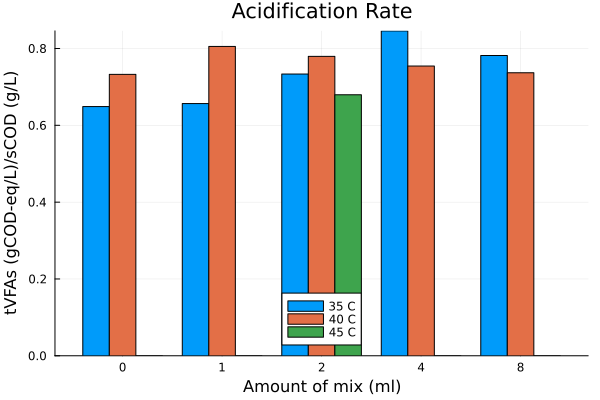
\includegraphics[width=.9\linewidth]{../plots/35_40_45_comp/acidification_comp.png}
\caption{\label{fig:orgf38ec20}Οξίνιση των Αντιδραστήρων}
\end{figure}

Από το διάγραμμα αυτό παρατηρείται πως το πείραμα στους 40 \(^oC\) έχει καλύτερη οξίνιση σε χαμηλές ποσότητες \acrshort{mix}, ενώ το πείραμα στους 35 \(^oC\) είναι καλύτερο στις υψηλότερες ποσότητες. Το δοκιμαστικό πείραμα στους 45 \(^oC\) δεν έχει πάρα πολύ υψηλό βαθμό οξίνισης.

Το δεύτερο συγκεντρωτικό κριτήριο το οποίο εξετάστηκε είναι ο λόγος \[ \frac{\text{tVFAs$_{final}$ - \text{tVFAs$_{initial}$}}}{\text{tSugars$_{final}$} -  \text{tSugars$_{initial}$}} \] ο οποίος λόγος εξετάζει την απόδοση μετατροπής των σακχάρων σε προϊόντα και θεωρείται ένα ακόμη χρήσιμο κριτήριο. Τα σχετικά αποτελέσματα παρουσιάζονται στο Σχήμα .

\begin{figure}[htbp]
\centering
\includegraphics[width=.9\linewidth]{../plots/35_40_45_comp/Δprod.png}
\caption{Απόδοση μετατροπής σακχάρων σε οξεογενή προϊόντα}
\end{figure}

Από το διάγραμμα αυτό, παρατηρείται πως το πείραμα στους 40 \(^oC\) έχει σε κάθε περίπτωση την καλύτερη απόδοση μετατροπής, ενώ οι 45 \(^oC\) έχουν μάλλον την χειρότερη (καθώς η μία ποσότητα που εξετάστηκε έχει χαμηλότερη απόδοση από την αντίστοιχη στους 35 \(^oC\)). Αξίζει να σημειωθεί πως ακολουθείται μία παρόμοια τάση στις δύο θερμοκρασίες, όπου τα πειράματα με προσθήκη 1 ή 4 mL \acrshort{mix} έχουν χειρότερο αποτέλεσμα από τα 0, 2 και 8 mL \acrshort{mix}, ενώ τα 2 και 8 mL \acrshort{mix} φαίνεται να έχουν το ίδιο yield. Αξιοσημείωτο αποτέλεσμα είναι η απόδοση μετατροπής του πειράματος με 0 mL \acrshort{mix} στους 40 \(^oC\). Το πείραμα αυτό είχε πολύ χαμηλό αρχικό COD, αλλά κατά την ζύμωση, είχε καλύτερη απόδοση μετατροπής από τα άλλα πειράματα. Μία εξήγηση για αυτό είναι ότι παράχθηκαν περισσότερα προϊόντα, αλλά υπήρχαν πολύ λίγοι μικροοργανισμοί στο σύστημα, με αποτέλεσμα να μην καταναλωθεί κάποια ποσότητα τους, το οποίο θα μείωνε την μετατροπή.

Επίσης, αξίζει να σημειωθεί πως οι μετατροπές αυτές είναι κάτω από \(70 \%\) σε κάθε περίπτωση. Αυτό συμβαίνει επειδή τα σάκχαρα δεν παράγουν μόνο αυτά τα προϊόντα, αλλά και άλλες ενώσεις, όπως το διοξείδιο του άνθρακα και το υδρογόνο, ενώ κάποια ποσότητα τους χρησιμοποιείται και για την ανάπτυξη της βιομάζας των μικροοργανισμών. Οπότε, δεν θεωρείται το καλύτερο κριτήριο για την διεργασία αυτή, παρότι είναι μία ενδιαφέρουσα μέτρηση.

\section{Ανάλυση Ευαισθησίας}
\label{sec:org11d4b26}
Από το Σχήμα \ref{fig:org5fc1157}, υπάρχει η ένδειξη πως η θερμοκρασία παίζει ένα πάρα πολύ σημαντικό ρόλο στη ζύμωση καθώς από τις 8 επιδράσεις, στις 4 πρώτες, οι 3 είναι θερμοκρασιακές, με την επίδραση της αιθανόλης να είναι η σημαντικότερη. Εκτός όμως από την αρνητική αυτή επίδραση, τα άλλα 3 μεταβολικά προϊόντα επηρεάζονται θετικά από την θερμοκρασία. Από την άποψη της ποσότητας \acrshort{mix}, φαίνεται πως το γαλακτικό έχει μία πολύ μεγάλη θετική επίδραση, το οξικό μία αρνητική επίδραση ενώ τα άλλα 2 δείχνουν να επηρεάζονται αμελητέα από την ποσότητα του \acrshort{mix}.

Όπως διαπιστώθηκε από το Σχήμα \ref{fig:orgdb103e7} η αρνητική επίδραση του οξικού από την ποσότητα \acrshort{mix} οφείλεται μόνο στην χαμηλή θερμοκρασία. Οπότε, η λειτουργία στους 40 \(^oC\) θεωρείται πιο επιθυμητή στην περίπτωση που η διεργασία αυτή είναι προ-επεξεργασία για αναερόβια χώνευση, επειδή η αύξηση της συγκέντρωσης του οξικού οξέος είναι επιθυμητή. (Σίγουρα θέλω και κάποια σχόλια για το γιατί δεν κάναμε άλλο πείραμα στους 45 \(^oC\), αλλά δεν έχω τα κατάλληλα αποτελέσματα ήδη γραμμένα νμζ).

Για την ποσότητα του \acrshort{mix} θεωρήθηκε πως η βέλτιστη ποσότητα είναι 2 mL \acrshort{mix} καθώς σε παραπάνω ποσότητες η βελτίωση είναι αρκετά μικρή. Αυτό φαίνεται ιδιαίτερα ξεκάθαρα στο Σχήμα \ref{fig:org99640c0} όπου καμία ένωση δεν έχει θετική ευαισθησία στο εξεταζόμενο εύρος. Όμως, η διαφορά από το 1 mL στα 2 mL είναι στα περισσότερα πειράματα σημαντική.

\section{Υδρόλυση σε Πιλοτική Κλίμακα}
\label{sec:org0a8439b}
Τα αποτελέσματα των πειραμάτων της πιλοτικής κλίμακας αναλύθηκαν κυρίως ως προς την απόδοση της υδρόλυσης, η οποία μετριέται από τον λόγο διαλυτού με ολικό \acrshort{cod}. Για τον πρώτο πειραματικό κύκλο, ο λόγος αυτός ήταν \(46.1 \pm 12.2 \%\).

Έπειτα, εξετάστηκε η μεταβολή της ποσότητας νερού που προστίθεται στον αντιδραστήρα. Ο λόγος sCOD/tCOD στην περίπτωση αυτή ήταν \(39.2 \pm 10.4 \%\) το οποίο φαινομενικά φαίνεται χειρότερο από το προηγούμενο, αλλά συγκρίνοντας τα με ένα t-test, φαίνεται πως δεν μπορεί να προκύψει ασφαλές συμπέρασμα για την επίδραση της αραίωσης στην υδρόλυση/βιοαποδόμηση (p-Value = 0.14). 

Τέλος, στο τρίτο πείραμα διπλασιάστηκε η ποσότητα του \acrshort{mix} που προστίθεται και βρέθηκε πως ο λόγος sCOD/tCOD ήταν \(32.7 \pm 10.3 \%\), μείωση η οποία είναι στατιστικά σημαντική σε σχέση με τις προηγούμενες τιμές (p-Value = 0.0002 και 0.0011 σε t-test με το 1ο και 2ο πείραμα αντίστοιχα). Οπότε, είναι ασφαλές να προκύψει το συμπέρασμα ότι η προσθήκη παραπάνω από 5 mL \acrshort{mix}/kg \acrshort{fw} δεν βοηθάει την υδρόλυση.

Ένα πιθανό αίτιο για αυτό είναι πως προστίθενται περισσότεροι μικροοργανισμοί, οι οποίοι καταναλώνουν διαλυτό \acrshort{cod} για να τραφούν. Ένα μεγάλο ποσοστό της τροφής αυτής μετατρέπεται στα οξεογενή προϊόντα, αλλά αν οι μικροοργανισμοί αυξηθούν πολύ, αρχίζει να παρατηρείται και η μείωση στο \acrshort{cod}. Αντίθετα, η υδρόλυση μπορεί να γίνεται κορεσμένη σε ένζυμα (δηλαδή να μην περιορίζεται πλέον από την ποσότητα αυτών) σε ποσότητα κοντά στα 5 mL \acrshort{mix}/kg \acrshort{fw}. Αυτό δείχνει μία ένδειξη πως παρότι στα εργαστηριακά πειράματα φάνηκε πιο αποτελεσματική η ποσότητα 10 mL \acrshort{mix}/kg \acrshort{fw} λόγω της βέλτιστης οξεογένεσης, αυτό μπορεί να μην συνάδει με το βέλτιστο της υδρόλυσης. Οπότε, έχει αρκετό ενδιαφέρον να βρεθεί τι από τα δύο είναι πιο σημαντικό για την \acrshort{ad}.

Βέβαια, υπάρχει και πιθανότητα αυτό να είναι μία διαφορά μεταξύ της εργαστηριακής και της πιλοτικής κλίμακας και στην κλίμακα αυτή, η ποσότητα 5 mL \acrshort{mix}/kg \acrshort{fw} να έχει και καλύτερη οξεογένεση. Για τον σκοπό αυτόν, τα 2 αυτά δείγματα αναλύθηκαν με \acrshort{hplc} για να διαλευκανθεί αυτό το θέμα.

\section{Αναερόβια Χώνευση}
\label{sec:orgc7f15c9}
Από τα πειράματα αναερόβιας χώνευσης, είναι εμφανές πως τα υδρολύματα τα οποία παρασκευάστηκαν με προσθήκη 1 ή 2 mL \acrshort{mix} είχαν την καλύτερη απόδοση. Μία σημαντική παρατήρηση ήταν ότι τα αποτελέσματα των 3 κύκλων που έγιναν με τα εργαστηριακά υδρολύματα ήταν σε πλήρη αντιστοιχία.

Γενικά, τα πειράματα με υδρόλυμα με 2 mL \acrshort{mix} είχαν τον χαμηλότερο χρόνο καθυστέρησης από κάθε πείραμα, ο οποίος σε κάποιες περιπτώσεις ήταν και μηδενικός, καθώς και την μεγαλύτερη \acrshort{sma}. Αυτό δείχνει πως τα υδρολύματα αυτά είχαν την καλύτερη οξεογενετική ζύμωση και μπορούσε να ξεκινήσει ταχύτατα η μεθανογένεση, κάτι το οποίο έρχεται σε συμφωνία με τα αποτελέσματα των πειραμάτων υδρόλυσης.

Όμως, παρότι ισχύει αυτό, το υδρόλυμα με 1 mL \acrshort{mix}, παράγει σε κάθε περίπτωση περισσότερο μεθάνιο αν οι χωνεύσεις λειτουργήσουν μέχρι την στιγμή που ο ρυθμός γίνεται σχεδόν 0. Και αυτό έρχεται σε συμφωνία με τα παραπάνω αποτελέσματα, καθώς είχε παρατηρηθεί καλύτερη υδρόλυση (περισσότερο \acrshort{scod}) στα πειράματα αυτά. Οπότε, αν δοθεί ο χρόνος που χρειάζεται για να ξεκινήσει η μεθανογένεση στα πειράματα αυτά, θα είναι πιο αποτελεσματικά.

Αξιοσημείωτη είναι και η πάρα πολύ χαμηλή παραγωγή μεθανίου από το ανεπεξέργαστο \acrshort{fw}, η οποία είναι περίπου 4-5 φορές χαμηλότερη από αυτή του υδρολύματος στο οποίο προστέθηκε 1 mL \acrshort{mix}. Ως συμπέρασμα, διαπιστώθηκε ότι το ανεπεξέργαστο \acrshort{fw} δεν είναι ένα καλό υπόστρωμα για την παραγωγή μεθανίου, καθώς η παραγωγή είναι ασταθείς και το συνολικό μεθάνιο λίγο. Συγκεκριμένα, παρατηρήθηκε υπερβολική οξίνιση του αντιδραστήρα σε έναν από τους κύκλους, στον οποίο χρησιμοποιήθηκε αρκετά αλκαλική λάσπη \ref{tab:orgb9a5457}.

Τέλος, έγιναν και οι δοκιμές με τα πιλοτικά υδρολύματα, οι οποίες έδειξαν ότι τα αποτελέσματα που προέκυψαν στην πιλοτική κλίμακα είναι σε συμφωνία με τα εργαστηριακά, καθώς και σε αυτά το υδρόλυμα το οποίο είχε τροφοδοσία 10 mL \acrshort{mix}/kg \acrshort{fw}, αναλογία η οποία αντιστοιχεί στα 2 mL της εργαστηριακής κλίμακας, ήταν πιο γρήγορο στην αρχή αλλά εν τέλει παρήγαγε λιγότερο μεθάνιο από το υδρόλυμα με 5 mL \acrshort{mix}/kg \acrshort{fw}, το οποίο είναι αντίστοιχο του 1 mL της εργαστηριακής κλίμακας.

Για την σύγκριση των αποτελεσμάτων με την βιβλιογραφία, επιλέχθηκαν κάποιες δημοσιέυσεις οι οποίες ασχολούνται με αναερόβια χώνευση υπολειμμάτων τροφών και έκαναν μοντελοποίηση με το μοντέλο Gompertz, για να είναι συγκρίσιμα τα αποτελέσματα. Όμως, βρέθηκαν δημοσιεύσεις με διαφορετική προεπεξεργασία, όπως ενζυμική υδρόλυση \textsuperscript{\citeprocitem{32}{32}}, αναερόβια χώνευση σε 2 στάδια \textsuperscript{\citeprocitem{76}{76}}, υπέρηχοι και μικροκύματα \textsuperscript{\citeprocitem{112}{112}} ή ακόμη και καμία προεπεξεργασία \textsuperscript{\citeprocitem{97}{97},\citeprocitem{113}{113}}, για να μπορέσει να εξεταστεί η επίδραση της προεπεξεργασίας στα αποτελέσματα. Μία από τις σημαντικότερες λειτουργικές συνθήκες στην αναερόβια χώνευση είναι ο λόγος \acrfull{si}. Μάλιστα, βρέθηκαν και κάποιες μελέτες που σύγκριναν διαφορετικά επίπεδα \textsuperscript{\citeprocitem{97}{97},\citeprocitem{100}{100}}, το οποίο δείχνει την σημασία του λόγου αυτού.

Στην εργασία αυτή, εξετάστηκε η αναερόβια χώνευση σε 2 στάδια με το πρώτο στάδιο να έχει ενεργά ένζυμα για την βελτιστοποίηση της υδρόλυσης. Στο δεύτερο στάδιο χρησιμοποιήθηκαν χαμηλές αναλογίες \acrshort{si} (0.06 και 0.02 gCOD/gVS), το οποίο προσφέρει κάποια πλεονεκτήματα, όπως αναφέρθηκε στο πειραματικό μέρος ( \autoref{sec:exp-ad}). Ως αποτέλεσμα, η άμεση σύγκριση ήταν σχετικά δύσκολη. Όπως και αναμενόταν μετά την επιλογή των λόγων \acrshort{si} αυτών, τα πειράματα που έγιναν είχαν χαμηλή συνολική παραγωγή μεθανίου και πιο αργούς ρυθμούς παραγωγής από τα περισσότερα άρθρα στη βιβλιογραφία, όμως, οι χρόνοι καθυστέρησης, και γενικότερα η διάρκεια των πειραματικών κύκλων ήταν μικρότερη.

Ένα από τα καλύτερα πειράματα που διεξάχθηκαν στην μελέτη αυτή ήταν το υδρόλυμα εργαστηριακής κλίμακας με προσθήκη 2 mL \acrshort{mix}, με χρήση της λάσπης 2. Αυτό είχε παραγωγή 30 mL CH\textsubscript{4}, με ρυθμό \(3~ \frac{mL}{\text{gVS} \cdot \text{day}}\) ή \(12.5 ~ \frac{mL}{day}\) ή \(125 ~ \frac{mL}{\text{gCOD} \cdot \text{day}}\) (είναι απαραίτητα και τα 3 καθώς κάθε δεν χρησιμοποιείται η ίδια έκφραση σε κάθε άρθρο) και μηδενικό χρόνο καθυστέρησης. Στην βιβλιογραφία, οι ρυθμοί παραγωγής είναι συχνά στην τάξη των 15-45 \(\frac{mL}{\text{gVS} \cdot \text{day}}\) \textsuperscript{\citeprocitem{32}{32},\citeprocitem{87}{87},\citeprocitem{100}{100}}, όμως κάποιες μελέτες, οι οποίες είχαν και κοντινότερες λειτουργικές συνθήκες σε αυτές που εξετάστηκαν στην εργασία αυτή, είχαν αντίστοιχους ρυθμούς. Για παράδειγμα, μία μελέτη που ακολούθησε αρκετά παρόμοια διαδικασία για την μέτρηση της παραγωγής μεθανίου, αλλά σε ανεπεξέργαστο \acrshort{fw}, βρήκε έναν ρυθμό \(2.8 ~ \frac{ml}{gVS \cdot day}\) \textsuperscript{\citeprocitem{113}{113}} . Μία άλλη, η οποία εξέτασε διαφορετικούς τύπους οξεογενούς ζύμωσης (ανάλογα με το pH), βρήκε ως μέγιστο ρυθμό τα \(110 ~ \frac{ml}{gCOD \cdot day}\) σε pH 4.7, το οποίο είναι χαμηλότερο από τον ρυθμό της προτεινόμενης επεξεργασίας. Ακόμη, σε pH 4.0, το οποίο είναι αντίστοιχο με αυτό που εξετάστηκε στη μελέτη αυτή, ο ρυθμός ήταν ακόμη χαμηλότερος, στα \(90.1 ~ \frac{ml}{gCOD \cdot day}\). Ακόμη, ως προς τους χρόνους καθυστέρησης, αυτοί κυμαίνονται από μερικές ώρες \textsuperscript{\citeprocitem{32}{32},\citeprocitem{76}{76}} εώς και κάποιες μέρες \textsuperscript{\citeprocitem{87}{87},\citeprocitem{97}{97}}. Αναμένεται πως τα πειράματα με τόσο χαμηλό \acrshort{si} θα έχουν χαμηλότερους χρόνους καθυστέρησης, αλλά ειδικά επειδή η τιμή 0 είναι πολύ χαμηλότερη από άλλες συνθήκες του ίδιου πειραματικού κύκλου, θεωρείται πως η βελτιστοποιημένες συνθήκες υδρόλυσης με την προτεινόμενη διεργασία, μπορούν να οδηγήσουν σε ένα πολύ πιο αποτελεσματικό υπόστρωμα για \acrshort{ad} σε σχέση με άλλες αντίστοιχες διεργασίες.

\chapter{Συμπεράσματα και Προτάσεις}
\label{sec:org2751817}
\label{sec:conclusion}

Τα \acrfull{fw} αποτελούν ένα πολύ σοβαρό πρόβλημα της σημερινής κοινωνίας και η διαχείριση τους είναι πολύ σημαντική, λόγω του υψηλού οργανικού φορτίου που έχουν. Η διαχείριση τους με συμβατικές μεθόδους όπως η διάθεση τους σε \acrshort{xyta} δεν θεωρείται βιώσιμη καθώς δεν εκμεταλλεύεται το φορτίο αυτό, και μάλιστα οδηγεί και σε ανεξέλεγκτες εκπομπές μεθανίου. Για τον λόγο αυτόν, είναι επιτακτική η ανάγκη ανάπτυξης τεχνολογιών διαχείρισης \acrshort{fw}, η οποίες να είναι εύκολες στην εφαρμογή και την κλιμάκωση. Στην εργασία αυτή επιλέχθηκε η \acrfull{ad}, λόγω του υψηλού \acrshort{trl} της και της παραγωγής ενός πολύ χρησιμού ενεργειακού φορέα, του μεθανίου, το οποίο παράγεται ελεγχόμενα και μπορεί να αποθηκευτεί. Μέσω μίας βιβλιογραφικής ανασκόπησης, βρέθηκαν τα προβλήματα της διεργασίας αυτής, όπως η μειωμένη απόδοση υδρόλυσης κατά την χώνευση και η αστάθεια της όταν λειτουργεί σε μεγάλο ρυθμό φόρτισης. Η διεξαγωγή της \acrshort{ad} σε 2 στάδια λύνει τα προβλήματα αυτά.

Επιλέχθηκε η χρήση ενός εμπορικού σκευάσματος ενζύμων και μικροοργανισμών (μιξ) χαμηλής τιμής (PROGEN L 100) για το πρώτο στάδιο, καθώς επιτρέπει την αποτελεσματική ενζυμική υδρόλυση του υποστρώματος, σε ένα χαμηλό σχετικά κόστος, ενώ ταυτόχρονα μπορεί να γίνει και η οξεογενή ζύμωση. Η διεργασία αυτή βελτιστοποιήθηκε σε εργαστηριακή κλίμακα με αντιδραστήρες 1 L, ενώ οι καλύτερες συνθήκες εξετάστηκαν και σε πιλοτικό αντιδραστήρα όγκου 300 L για να εξεταστεί η εφικτότητα της κλιμάκωσης της διεργασίας αυτής. Διαπιστώθηκε πως η βέλτιστη διάρκεια των πειράματων ήταν 72 ώρες, ενώ η διεργασία ήταν πιο αποτελεσματική στους 40 \(^oC\), καθώς στους 35 \(^oC\) παραγόταν πολύ αιθανόλη εις βάρος του οξικού οξέος, το οποίο είναι το θεωρητικά ιδανικό υπόστρωμα για την διεργασία. Ως προς την ποσότητα του μιξ που προστέθηκε σε κάθε πείραμα, βρέθηκε πως η προσθήκη 10 mL μιξ/kg \acrshort{fw} είχε την καλύτερη απόδοση παραγωγής οξεογενών προϊόντων όπως το οξικό και το γαλακτικό οξύ μετά από μία ανάλυση ευαισθησίας. Όμως, αν προστεθούν μόνο 5 mL μιξ/kg \acrshort{fw}, η υδρόλυση/βιοαποδόμηση είναι πιο αποτελεσματική. Συγκεκριμένα, βρέθηκε πως ο λόγος sCOD/tCOD ήταν \(46.08 \pm 12.17\), ενώ στην περίπτωση των 10 mL μιξ/kg \acrshort{fw} ήταν \(32.72 \pm 10.30\) τιμή η οποία είναι χαμηλότερη με στατιστική βεβαιότητα (p-Value = 0.0002). Αυτό συμβαίνει επειδή στην περίπτωση των 10 mL/kg \acrshort{fw}, υπάρχουν περισσότεροι μικροοργανισμοί και καταναλώνεται κάποιο από το παραγόμενο \acrshort{cod}, ενώ η ποσότητα ενζύμων που απαιτείται για την αποτελεσματική υδρόλυση/βιοαποδόμηση μπορεί να επιτευχθεί ακόμη και στα 5 mL μιξ/kg \acrshort{fw}.

Το δεύτερο στάδιο της \acrshort{ad}, το οποίο περιέχει την μεθανογένεση έγινε μόνο σε εργαστηριακή κλίμακα σε αντιδραστήρες 0.5 L. Τα συμπεράσματα της υδρόλυσης/βιοαποδόμησης επαληθεύτηκαν κατά το στάδιο αυτό, καθώς τα υδρολύματα με 5 mL μιξ/kg \acrshort{fw} είχαν την μεγαλύτερη παραγωγή μεθανίου, όμως αυτά με 10 mL μιξ/kg \acrshort{fw} είχαν υψηλότερους ρυθμούς και μικρότερο χρόνο καθυστέρησης, επειδή είχαν πιο αποτελεσματική ζύμωση, και το υπόστρωμα ήταν πιο εύκολο στην μεθανογένεση. Τα αποτελέσματα αυτά επαληθεύτηκαν με λάσπη από 3 διαφορετικές πηγές και χρησιμοποιώντας υδρολύματα από πειράματα εργαστηριακής αλλά και πιλοτικής κλίμακας. Ακόμη, η παραγωγή αυτή συγκρίθηκε με αυτήν των ανεπεξέργαστων \acrshort{fw}, όπου παρατηρήθηκε αστάθεια της διεργασίας και οξίνιση σε κάποιες περιπτώσεις, αλλά και ακόμη όταν δεν έγινε αυτό, η παραγωγή ήταν περίπου 4-5 φορές μικρότερη από την μέγιστη παραγωγή μεθανίου μετά το στάδιο υδρόλυσης που χρησιμοποιήθηκε.

Έτσι, διαπιστώθηκε πως η διεργασία υδρόλυσης/βιοαποδόμησης με το εμπορικό σκεύασμα PROGEN L 100 είναι μία πολύ αποτελεσματική διεργασία για την βελτίωση της απόδοσης και της σταθερότητας της \acrshort{ad} σε εργαστηριακή αλλά και σε πιλοτική κλίμακα, ενώ είναι μία προεπεξεργασία χαμηλού κόστους. Η βέλτιστη δοσολογία του σκευάσματος για γρήγορη \acrshort{ad} είναι 10 mL μιξ/kg \acrshort{fw}, ενώ για μεγιστοποίηση της παραγωγής μεθανίου - αλλά λίγο πιο αργό ρυθμό - προτείνεται η δοσολογία 5 mL μιξ/kg \acrshort{fw}.

Παρόλη την πρόοδο που υπήρξε στα πλαίσια της εργασίας αυτής, η προτεινόμενη διεργασία έχει ακόμη κάποια ερευνητικά κενά τα οποία προτείνεται να καλυφθούν σε επόμενες ερευνητικές εργασίες. Ένα από τα σημαντικότερα αντικείμενα προς μελέτη είναι η επίδραση του pH στην διεργασία υδρόλυσης/βιοαποδόμησης. Με βάση την βιβλιογραφία, το pH είναι από τους σημαντικότερους παράγοντες που επηρεάζουν την διεργασία και η εύρεση μίας βέλτιστης τιμής αυτού μπορεί να συνεισφέρει σημαντικά στην απόδοση της. Στην παρούσα μελέτη επιλέχθηκε η διεξαγωγή των πειραμάτων χωρίς μεταβολή του pH, για να μην αυξηθεί περαιτέρω η πολυπλοκότητα της, αλλά αυτό είναι σίγουρα ένα αντικείμενο προς συζήτηση. Ως προς άλλες λειτουργικές συνθήκες, θα ήταν ενδιαφέρουσα η εξέταση ψυχρόφιλων ή θερμόφιλων θερμοκρασιών πέρα από την μεσοφιλή περιοχή που εξετάστηκε στην εργασία αυτή, καθώς η θερμοκρασία παίζει βασικό ρόλο στις μικροβιακές δράσεις (παρόλο που αναμένεται πως η μεσόφιλη περιοχή είναι ιδανική) αλλά και η μελέτη της διεργασίας σε πιο ελεγχόμενες συνθήκες αερισμού ή σε πλήρως αναερόβιες συνθήκες για να παρατηρηθεί αν όντως ο μικροαερισμός που επιβλήθηκε βοήθησε την διεργασία και αν υπάρχει περιθώριο για περαιτέρω βελτίωση από αυτό. Ως προς το δεύτερο στάδιο της διεργασίας, υπάρχει αρκετό ενδιαφέρον στο να γίνει μία αναλυτική μελέτη της αναερόβιας χώνευσης των υδρολυμάτων αυτών σε πιλοτική μονάδα συνεχούς λειτουργίας καθώς εξετάστηκε η κλιμάκωση της υδρόλυσης/βιοαποδόμησης, αλλά όχι της αναερόβιας χώνευσης. Θεωρείται πως τα συμπεράσματα θα είναι αντίστοιχα, αλλά θα είχε ενδιαφέρον να γίνει για την ολοκλήρωση της διεργασίας σε πιλοτική κλίμακα. 

Τέλος, ένα αντικείμενο αρκετού ερευνητικού ενδιαφέροντος γύρω από την διεργασία αυτή είναι η χρήση του παραγόμενου υδρολύματος, το οποίο είναι πλούσιο σε \acrfull{vfa} ως πλατφόρμα για παραγωγή βιο-προϊόντων στη λογική ενός βιοδιυλιστηρίου. Η ενέργεια είναι ένα πολύ σημαντικό ζήτημα και η μετάβαση σε πιο πράσινες πηγές ενέργειας όπως το βιοαέριο είναι αρκετά σημαντική. Όμως, ακόμη μεγαλύτερο πρόβλημα στην πράσινη μετάβαση αποτελούν τα προϊόντα τα οποία παράγονται από το πετρέλαιο. Το υδρόλυμα αυτό αποτελεί ένα φθηνό υπόστρωμα, το οποίο έχει παραχθεί με πράσινο τρόπο από ένα απόβλητο. Περιέχει χρήσιμες ενώσεις (οξικό οξύ, προπιονικό οξύ, γαλακτικό οξύ και αιθανόλη, ενώ με αλλαγή των λειτουργικών συνθηκών θεωρείται πως θα μπορέσουν να παραχθούν και άλλες) οι οποίες μπορούν να ανακτηθούν ως έχουν, καθώς όλα τα προϊόντα αυτά παράγονται συμβατικά από το πετρέλαιο και έχουν μία σημαντική αγορά είτε για άμεση χρήση ή ως χημικά ενδιάμεσα για την παραγωγή άλλων ενώσεων. Εναλλακτικά, μπορούν να χρησιμοποιηθούν χωρίς διαχωρισμό για παραγωγή προϊόντων όπως τα \acrfull{mcfa} ή ακόμη και για την παραγωγή βιοπλαστικών όπως οι \acrfull{pha}, κάτι που θα είχε ιδιαίτερο ενδιαφέρον για την αντικατάσταση των πετρελαϊκών πρώτων υλών.

\part*{Βιβλιογραφία}
\label{sec:orgf13a13b}
\hypertarget{citeproc_bib_item_1}{(1) Ishangulyyev, R.; Kim, S.; Lee, S. H. Understanding Food Loss and Waste–-Why Are We Losing and Wasting Food? \textit{Foods} \textbf{2019}, \textit{8} (8), 297. \url{https://doi.org/10.3390/foods8080297}.}

\hypertarget{citeproc_bib_item_2}{(2) Taheri, M. E.; Salimi, E.; Saragas, K.; Novakovic, J.; Barampouti, E. M.; Mai, S.; Malamis, D.; Moustakas, K.; Loizidou, M. Effect of Pretreatment Techniques on Enzymatic Hydrolysis of Food Waste. \textit{Biomass conversion and biorefinery} \textbf{2021}, \textit{11} (2), 219–226. \url{https://doi.org/10.1007/s13399-020-00729-7}.}

\hypertarget{citeproc_bib_item_3}{(3) Statista - The Statistics Portal. https://www.statista.com/ November 2023.}

\hypertarget{citeproc_bib_item_4}{(4) Pardo, R.; Taboada-Ruiz, L.; Fuente, E.; Ruiz, B.; Díaz-Somoano, M.; Calvo, L. F.; Paniagua, S. Exploring the Potential of Conventional and Flash Pyrolysis Methods for the Valorisation of Grape Seed and Chestnut Shell Biomass from Agri-Food Industry Waste. \textit{Biomass and bioenergy} \textbf{2023}, \textit{177}, 106942. \url{https://doi.org/10.1016/j.biombioe.2023.106942}.}

\hypertarget{citeproc_bib_item_5}{(5) Usmani, Z.; Sharma, M.; Awasthi, A. K.; Sharma, G. D.; Cysneiros, D.; Nayak, S. C.; Thakur, V. K.; Naidu, R.; Pandey, A.; Gupta, V. K. Minimizing Hazardous Impact of Food Waste in a Circular Economy – Advances in Resource Recovery through Green Strategies. \textit{Journal of hazardous materials} \textbf{2021}, \textit{416}, 126154. \url{https://doi.org/10.1016/j.jhazmat.2021.126154}.}

\hypertarget{citeproc_bib_item_6}{(6) Xu, S.; Zhu, S.; Li, C.; Bu, J.; Wei Tiong, Y.; Sharma, P.; Kong, W.; Shao, C.; Xie, H.; Wah Tong, Y. Succession of Biochar in Integrated Pyrolysis, Anaerobic Digestion, and Solid–State Fermentation towards Closed Loop Valorization of Food Waste. \textit{Fuel} \textbf{2024}, \textit{369}, 131719. \url{https://doi.org/10.1016/j.fuel.2024.131719}.}

\hypertarget{citeproc_bib_item_7}{(7) Infurna, G.; Caruso, G.; Dintcheva, N. T. Sustainable Materials Containing Biochar Particles: A Review. \textit{Polymers} \textbf{2023}, \textit{15} (2), 343. \url{https://doi.org/10.3390/polym15020343}.}

\hypertarget{citeproc_bib_item_8}{(8) Murugesan, P.; Raja, V.; Dutta, S.; Moses, J. A.; Anandharamakrishnan, C. Food Waste Valorisation via Gasification – A Review on Emerging Concepts, Prospects and Challenges. \textit{Science of the total environment} \textbf{2022}, \textit{851}, 157955. \url{https://doi.org/10.1016/j.scitotenv.2022.157955}.}

\hypertarget{citeproc_bib_item_9}{(9) Udaeta, M.; Burani, G.; Arzabe Maure, J. O.; Oliva, C. Economics of Secondary Energy from GTL Regarding Natural Gas Reserves of Bolivia. \textit{Energy policy} \textbf{2007}, \textit{35}, 4095–4106. \url{https://doi.org/10.1016/j.enpol.2007.02.014}.}

\hypertarget{citeproc_bib_item_10}{(10) Cerda, A.; Artola, A.; Font, X.; Barrena, R.; Gea, T.; Sánchez, A. Composting of Food Wastes: Status and Challenges. \textit{Bioresource technology} \textbf{2018}, \textit{248}, 57–67. \url{https://doi.org/10.1016/j.biortech.2017.06.133}.}

\hypertarget{citeproc_bib_item_11}{(11) Ma, C.; Liu, J.; Ye, M.; Zou, L.; Qian, G.; Li, Y.-Y. Towards Utmost Bioenergy Conversion Efficiency of Food Waste: Pretreatment, Co-Digestion, and Reactor Type. \textit{Renewable and sustainable energy reviews} \textbf{2018}, \textit{90}, 700–709. \url{https://doi.org/10.1016/j.rser.2018.03.110}.}

\hypertarget{citeproc_bib_item_12}{(12) Xu, F.; Li, Y.; Ge, X.; Yang, L.; Li, Y. Anaerobic Digestion of Food Waste – Challenges and Opportunities. \textit{Bioresource technology} \textbf{2018}, \textit{247}, 1047–1058. \url{https://doi.org/10.1016/j.biortech.2017.09.020}.}

\hypertarget{citeproc_bib_item_13}{(13) Anwar Saeed, M.; Ma, H.; Yue, S.; Wang, Q.; Tu, M. Concise Review on Ethanol Production from Food Waste: Development and Sustainability. \textit{Environmental science and pollution research} \textbf{2018}, \textit{25} (29), 28851–28863. \url{https://doi.org/10.1007/s11356-018-2972-4}.}

\hypertarget{citeproc_bib_item_14}{(14) Roukas, T.; Kotzekidou, P. From Food Industry Wastes to Second Generation Bioethanol: A Review. \textit{Reviews in environmental science and bio/technology} \textbf{2022}, \textit{21} (1), 299–329. \url{https://doi.org/10.1007/s11157-021-09606-9}.}

\hypertarget{citeproc_bib_item_15}{(15) Yasin, N.; Mumtaz, T.; Hassan, M.; Abd Rahman, N. Food Waste and Food Processing Waste for Biohydrogen Production: A Review. \textit{Journal of environmental management} \textbf{2013}, \textit{130}, 375–385. \url{https://doi.org/10.1016/j.jenvman.2013.09.009}.}

\hypertarget{citeproc_bib_item_16}{(16) Mohanakrishna, G.; Sneha, N. P.; Rafi, S. M.; Sarkar, O. Dark Fermentative Hydrogen Production: Potential of Food Waste as Future Energy Needs. \textit{Science of the total environment} \textbf{2023}, \textit{888}, 163801. \url{https://doi.org/10.1016/j.scitotenv.2023.163801}.}

\hypertarget{citeproc_bib_item_17}{(17) Rajesh Banu, J.; Godvin Sharmila, V. Review on Food Waste Valorisation for Bioplastic Production towards a Circular Economy: Sustainable Approaches and Biodegradability Assessment. \textit{Sustainable energy \& fuels} \textbf{2023}, \textit{7} (14), 3165–3184. \url{https://doi.org/10.1039/D3SE00500C}.}

\hypertarget{citeproc_bib_item_18}{(18) Pleissner, D.; Demichelis, F.; Mariano, S.; Fiore, S.; Navarro Gutiérrez, I.; Schneider, R.; Venus, J. Direct Production of Lactic Acid Based on Simultaneous Saccharification and Fermentation of Mixed Restaurant Food Waste. \textit{Journal of cleaner production} \textbf{2017}, \textit{143}, 615–623. \url{https://doi.org/10.1016/j.jclepro.2016.12.065}.}

\hypertarget{citeproc_bib_item_19}{(19) Mankins, J. C. TECHNOLOGY READINESS LEVELS. \textbf{1995}.}

\hypertarget{citeproc_bib_item_20}{(20) Franchetti, M. Economic and Environmental Analysis of Four Different Configurations of Anaerobic Digestion for Food Waste to Energy Conversion Using LCA for: A Food Service Provider Case Study. \textit{Journal of environmental management} \textbf{2013}, \textit{123}, 42–48. \url{https://doi.org/10.1016/j.jenvman.2013.03.003}.}

\hypertarget{citeproc_bib_item_21}{(21) Grippi, D.; Clemente, R.; Bernal, M. Chemical and Bioenergetic Characterization of Biofuels from Plant Biomass: Perspectives for Southern Europe. \textit{Applied sciences} \textbf{2020}, \textit{10}, 3571. \url{https://doi.org/10.3390/app10103571}.}

\hypertarget{citeproc_bib_item_22}{(22) Azbar, N.; Ursillo, P.; Speece, R. E. Effect of Process Configuration and Substrate Complexity on the Performance of Anaerobic Processes. \textit{Water research} \textbf{2001}, \textit{35} (3), 817–829. \url{https://doi.org/10.1016/S0043-1354(00)00318-3}.}

\hypertarget{citeproc_bib_item_23}{(23) Zoetemeyer, R. J.; Matthijsen, A. J. C. M.; Cohen, A.; Boelhouwer, C. Product Inhibition in the Acid Forming Stage of the Anaerobic Digestion Process. \textit{Water research} \textbf{1982}, \textit{16} (5), 633–639. \url{https://doi.org/10.1016/0043-1354(82)90084-7}.}

\hypertarget{citeproc_bib_item_24}{(24) Pohland, F. G.; Ghosh, S. Developments in Anaerobic Stabilization of Organic Wastes - The Two-Phase Concept. \textit{Environmental letters} \textbf{1971}. \url{https://doi.org/10.1080/00139307109434990}.}

\hypertarget{citeproc_bib_item_25}{(25) Zhang, J.; Loh, K.-C.; Li, W.; Lim, J. W.; Dai, Y.; Tong, Y. W. Three-Stage Anaerobic Digester for Food Waste. \textit{Applied energy} \textbf{2017}, \textit{194}, 287–295. \url{https://doi.org/10.1016/j.apenergy.2016.10.116}.}

\hypertarget{citeproc_bib_item_26}{(26) Wu, L.; Wei, W.; Liu, X.; Wang, D.; Ni, B.-J. Potentiality of Recovering Bioresource from Food Waste through Multi-Stage Co-digestion with Enzymatic Pretreatment. \textit{Journal of environmental management} \textbf{2022}, \textit{319}, 115777. \url{https://doi.org/10.1016/j.jenvman.2022.115777}.}

\hypertarget{citeproc_bib_item_27}{(27) Srisowmeya, G.; Chakravarthy, M.; Nandhini Devi, G. Critical Considerations in Two-Stage Anaerobic Digestion of Food Waste – A Review. \textit{Renewable and sustainable energy reviews} \textbf{2020}, \textit{119}, 109587. \url{https://doi.org/10.1016/j.rser.2019.109587}.}

\hypertarget{citeproc_bib_item_28}{(28) Kavitha, S.; Banu, J. R.; Priya, A. A.; Uan, D. K.; Yeom, I. T. Liquefaction of Food Waste and Its Impacts on Anaerobic Biodegradability, Energy Ratio and Economic Feasibility. \textit{Applied energy} \textbf{2017}, \textit{208}, 228–238. \url{https://doi.org/10.1016/j.apenergy.2017.10.049}.}

\hypertarget{citeproc_bib_item_29}{(29) Zhang, C.; Kang, X.; Wang, F.; Tian, Y.; Liu, T.; Su, Y.; Qian, T.; Zhang, Y. Valorization of Food Waste for Cost-Effective Reducing Sugar Recovery in a Two-Stage Enzymatic Hydrolysis Platform. \textit{Energy} \textbf{2020}, \textit{208}, 118379. \url{https://doi.org/10.1016/j.energy.2020.118379}.}

\hypertarget{citeproc_bib_item_30}{(30) Han, W.; Yan, Y.; Shi, Y.; Gu, J.; Tang, J.; Zhao, H. Biohydrogen Production from Enzymatic Hydrolysis of Food Waste in Batch and Continuous Systems. \textit{Scientific reports} \textbf{2016}, \textit{6} (1), 38395. \url{https://doi.org/10.1038/srep38395}.}

\hypertarget{citeproc_bib_item_31}{(31) Zou, L.; Wan, Y.; Zhang, S.; Luo, J.; Li, Y.-Y.; Liu, J. Valorization of Food Waste to Multiple Bio-Energies Based on Enzymatic Pretreatment: A Critical Review and Blueprint for the Future. \textit{Journal of cleaner production} \textbf{2020}, \textit{277}, 124091. \url{https://doi.org/10.1016/j.jclepro.2020.124091}.}

\hypertarget{citeproc_bib_item_32}{(32) Uçkun Kiran, E.; Trzcinski, A. P.; Liu, Y. Enhancing the Hydrolysis and Methane Production Potential of Mixed Food Waste by an Effective Enzymatic Pretreatment. \textit{Bioresource technology} \textbf{2015}, \textit{183}, 47–52. \url{https://doi.org/10.1016/j.biortech.2015.02.033}.}

\hypertarget{citeproc_bib_item_33}{(33) dos Santos Ferreira, J.; de Oliveira, D.; Maldonado, R. R.; Kamimura, E. S.; Furigo, A. Enzymatic Pretreatment and Anaerobic Co-Digestion as a New Technology to High-Methane Production. \textit{Applied microbiology and biotechnology} \textbf{2020}, \textit{104} (10), 4235–4246. \url{https://doi.org/10.1007/s00253-020-10526-x}.}

\hypertarget{citeproc_bib_item_34}{(34) Zhang, L.; Loh, K.-C.; Zhang, J.; Mao, L.; Tong, Y. W.; Wang, C.-H.; Dai, Y. Three-Stage Anaerobic Co-Digestion of Food Waste and Waste Activated Sludge: Identifying Bacterial and Methanogenic Archaeal Communities and Their Correlations with Performance Parameters. \textit{Bioresource technology} \textbf{2019}, \textit{285}, 121333. \url{https://doi.org/10.1016/j.biortech.2019.121333}.}

\hypertarget{citeproc_bib_item_35}{(35) Cekmecelioglu, D.; Uncu, O. N. Kinetic Modeling of Enzymatic Hydrolysis of Pretreated Kitchen Wastes for Enhancing Bioethanol Production. \textit{Waste management} \textbf{2013}, \textit{33} (3), 735–739. \url{https://doi.org/10.1016/j.wasman.2012.08.003}.}

\hypertarget{citeproc_bib_item_36}{(36) Cesaro, A.; Belgiorno, V. Pretreatment Methods to Improve Anaerobic Biodegradability of Organic Municipal Solid Waste Fractions. \textit{Chemical engineering journal} \textbf{2014}, \textit{240}, 24–37. \url{https://doi.org/10.1016/j.cej.2013.11.055}.}

\hypertarget{citeproc_bib_item_37}{(37) Graunke, R. E.; Wilkie, A. C. Examining the Mechanisms of Short-Term Solubilization of Ground Food Waste for High-Rate Anaerobic Digestion. \textit{International biodeterioration \& biodegradation} \textbf{2014}, \textit{86}, 327–333. \url{https://doi.org/10.1016/j.ibiod.2013.10.007}.}

\hypertarget{citeproc_bib_item_38}{(38) Wu, Y.; Wang, C.; Liu, X.; Ma, H.; Wu, J.; Zuo, J.; Wang, K. A New Method of Two-Phase Anaerobic Digestion for Fruit and Vegetable Waste Treatment. \textit{Bioresource technology} \textbf{2016}, \textit{211}, 16–23. \url{https://doi.org/10.1016/j.biortech.2016.03.050}.}

\hypertarget{citeproc_bib_item_39}{(39) Kim, D.-H.; Kim, M.-S. Development of a Novel Three-Stage Fermentation System Converting Food Waste to Hydrogen and Methane. \textit{Bioresource technology} \textbf{2013}, \textit{127}, 267–274. \url{https://doi.org/10.1016/j.biortech.2012.09.088}.}

\hypertarget{citeproc_bib_item_40}{(40) Chen, X.; Zheng, X.; Pei, Y.; Chen, W.; Lin, Q.; Huang, J.; Hou, P.; Tang, J.; Han, W. Process Design and Techno-Economic Analysis of Fuel Ethanol Production from Food Waste by Enzymatic Hydrolysis and Fermentation. \textit{Bioresource technology} \textbf{2022}, \textit{363}, 127882. \url{https://doi.org/10.1016/j.biortech.2022.127882}.}

\hypertarget{citeproc_bib_item_41}{(41) Moon, H. C.; Song, I. S. Enzymatic Hydrolysis of FoodWaste and Methane Production Using UASB Bioreactor. \textit{International journal of green energy} \textbf{2011}, \textit{8} (3), 361–371. \url{https://doi.org/10.1080/15435075.2011.557845}.}

\hypertarget{citeproc_bib_item_42}{(42) Jing, Y.; Li, F.; Li, Y.; Jin, P.; Zhu, S.; He, C.; Zhao, J.; Zhang, Z.; Zhang, Q. Statistical Optimization of Simultaneous Saccharification Fermentative Hydrogen Production from Corn Stover. \textit{Bioengineered} \textbf{2020}, \textit{11} (1), 428–438. \url{https://doi.org/10.1080/21655979.2020.1739405}.}

\hypertarget{citeproc_bib_item_43}{(43) Chen, Q.; Wu, W.; Qi, D.; Ding, Y.; Zhao, Z. Review on Microaeration-Based Anaerobic Digestion: State of the Art, Challenges, and Prospectives. \textit{Science of the total environment} \textbf{2020}, \textit{710}, 136388. \url{https://doi.org/10.1016/j.scitotenv.2019.136388}.}

\hypertarget{citeproc_bib_item_44}{(44) Suresh, T.; Sivarajasekar, N.; Balasubramani, K.; Ahamad, T.; Alam, M.; Naushad, M. Process Intensification and Comparison of Bioethanol Production from Food Industry Waste (Potatoes) by Ultrasonic Assisted Acid Hydrolysis and Enzymatic Hydrolysis: Statistical Modelling and Optimization. \textit{Biomass and bioenergy} \textbf{2020}, \textit{142}, 105752. \url{https://doi.org/10.1016/j.biombioe.2020.105752}.}

\hypertarget{citeproc_bib_item_45}{(45) Fang, H.; Shi, Y.; Li, D.; Song, L.; Li, Y.-Y.; Liu, R.; Yuan, D.; Niu, Q. Synergistic Co-Digestion of Waste Commercial Yeast and Chicken Manure: Kinetic Simulation, DOM Variation and Microbial Community Assessment. \textit{Renewable energy} \textbf{2020}, \textit{162}, 2272–2284. \url{https://doi.org/10.1016/j.renene.2020.10.038}.}

\hypertarget{citeproc_bib_item_46}{(46) Moon, H. C.; Song, I. S.; Kim, J. C.; Shirai, Y.; Lee, D. H.; Kim, J. K.; Chung, S. O.; Kim, D. H.; Oh, K. K.; Cho, Y. S. Enzymatic Hydrolysis of Food Waste and Ethanol Fermentation. \textit{International journal of energy research} \textbf{2009}, \textit{33} (2), 164–172. \url{https://doi.org/10.1002/er.1432}.}

\hypertarget{citeproc_bib_item_47}{(47) Zhang, C.; Ling, Z.; Huo, S. Anaerobic Fermentation of Pretreated Food Waste for Butanol Production by Co-Cultures Assisted with in-Situ Extraction. \textit{Bioresource technology reports} \textbf{2021}, \textit{16}, 100852. \url{https://doi.org/10.1016/j.biteb.2021.100852}.}

\hypertarget{citeproc_bib_item_48}{(48) Li, X.; Mettu, S.; Martin, G.; Ashokkumar, M.; Lin, C. Ultrasonic Pretreatment of Food Waste to Accelerate Enzymatic Hydrolysis for Glucose Production. \textit{Ultrasonics sonochemistry} \textbf{2019}, \textit{53}, 77–82. \url{https://doi.org/10.1016/j.ultsonch.2018.12.035}.}

\hypertarget{citeproc_bib_item_49}{(49) Uçkun Kiran, E.; Trzcinski, A. P.; Ng, W. J.; Liu, Y. Enzyme Production from Food Wastes Using a Biorefinery Concept. \textit{Waste and biomass valorization} \textbf{2014}, \textit{5} (6), 903–917. \url{https://doi.org/10.1007/s12649-014-9311-x}.}

\hypertarget{citeproc_bib_item_50}{(50) Soares, J. L.; Cammarota, M. C.; Gutarra, M. L. E.; Volschan, I. Jr. Reduction of Scum Accumulation through the Addition of Low-Cost Enzymatic Extract in the Feeding of High-Rate Anaerobic Reactor. \textit{Water science and technology} \textbf{2019}, \textit{80} (1), 67–74. \url{https://doi.org/10.2166/wst.2019.247}.}

\hypertarget{citeproc_bib_item_51}{(51) Arora, S.; Rani, R.; Ghosh, S. Bioreactors in Solid State Fermentation Technology: Design, Applications and Engineering Aspects. \textit{Journal of biotechnology} \textbf{2018}, \textit{269}, 16–34. \url{https://doi.org/10.1016/j.jbiotec.2018.01.010}.}

\hypertarget{citeproc_bib_item_52}{(52) Xiao, B.; Qin, Y.; Zhang, W.; Wu, J.; Qiang, H.; Liu, J.; Li, Y.-Y. Temperature-Phased Anaerobic Digestion of Food Waste: A Comparison with Single-Stage Digestions Based on Performance and Energy Balance. \textit{Bioresource technology} \textbf{2018}, \textit{249}, 826–834. \url{https://doi.org/10.1016/j.biortech.2017.10.084}.}

\hypertarget{citeproc_bib_item_53}{(53) Tang, Y.; Shigematsu, T.; Ikbal; Morimura, S.; Kida, K. The Effects of Micro-Aeration on the Phylogenetic Diversity of Microorganisms in a Thermophilic Anaerobic Municipal Solid-Waste Digester. \textit{Water research} \textbf{2004}, \textit{38} (10), 2537–2550. \url{https://doi.org/10.1016/j.watres.2004.03.012}.}

\hypertarget{citeproc_bib_item_54}{(54) Ramos, I.; Pérez, R.; Reinoso, M.; Torio, R.; Fdz-Polanco, M. Microaerobic Digestion of Sewage Sludge on an Industrial-Pilot Scale: The Efficiency of Biogas Desulphurisation under Different Configurations and the Impact of O2 on the Microbial Communities. \textit{Bioresource technology} \textbf{2014}, \textit{164}, 338–346. \url{https://doi.org/10.1016/j.biortech.2014.04.109}.}

\hypertarget{citeproc_bib_item_55}{(55) Lim, J. W.; Chen, C. .-L.; Ho, I. J. R.; Wang, J. .-Y. Study of Microbial Community and Biodegradation Efficiency for Single- and Two-Phase Anaerobic Co-Digestion of Brown Water and Food Waste. \textit{Bioresource technology} \textbf{2013}, \textit{147}, 193–201. \url{https://doi.org/10.1016/j.biortech.2013.08.038}.}

\hypertarget{citeproc_bib_item_56}{(56) Xu, S.; Selvam, A.; Wong, J. W. C. Optimization of Micro-Aeration Intensity in Acidogenic Reactor of a Two-Phase Anaerobic Digester Treating Food Waste. \textit{Waste management} \textbf{2014}, \textit{34} (2), 363–369. \url{https://doi.org/10.1016/j.wasman.2013.10.038}.}

\hypertarget{citeproc_bib_item_57}{(57) Nguyen, D.; Khanal, S. A Little Breath of Fresh Air into an Anaerobic System: How Microaeration Facilitates Anaerobic Digestion Process. \textit{Biotechnology advances} \textbf{2018}, \textit{36} (7), 1971–1983. \url{https://doi.org/10.1016/j.biotechadv.2018.08.007}.}

\hypertarget{citeproc_bib_item_58}{(58) Canul Bacab, F.; España Gamboa, E.; Ruiz Espinoza, J. E.; Leal-Bautista, R. M.; Tapia Tussell, R.; Domínguez Maldonado, J.; Canto Canché, B.; Alzate-Gaviria, L. Two Phase Anaerobic Digestion System of Municipal Solid Waste by Utilizing Microaeration and Granular Activated Carbon. \textit{Energies} \textbf{2020}, \textit{13} (4), 933. \url{https://doi.org/10.3390/en13040933}.}

\hypertarget{citeproc_bib_item_59}{(59) Lim, J. W.; Wang, J.-Y. Enhanced Hydrolysis and Methane Yield by Applying Microaeration Pretreatment to the Anaerobic Co-Digestion of Brown Water and Food Waste. \textit{Waste management} \textbf{2013}, \textit{33} (4), 813–819. \url{https://doi.org/10.1016/j.wasman.2012.11.013}.}

\hypertarget{citeproc_bib_item_60}{(60) Lim, J. W.; Chiam, J. A.; Wang, J.-Y. Microbial Community Structure Reveals How Microaeration Improves Fermentation during Anaerobic Co-Digestion of Brown Water and Food Waste. \textit{Bioresource technology} \textbf{2014}, \textit{171}, 132–138. \url{https://doi.org/10.1016/j.biortech.2014.08.050}.}

\hypertarget{citeproc_bib_item_61}{(61) Qiao, W.; Li, H.; Feng, K.; Liu, J. Oriented Fermentation of Food Waste towards High-Value Products: A Review. \textit{Energies} \textbf{2020}, \textit{13}, 5638. \url{https://doi.org/10.3390/en13215638}.}

\hypertarget{citeproc_bib_item_62}{(62) Feng, K.; Li, H.; Zheng, C. Shifting Product Spectrum by pH Adjustment during Long-Term Continuous Anaerobic Fermentation of Food Waste. \textit{Bioresource technology} \textbf{2018}, \textit{270}, 180–188. \url{https://doi.org/10.1016/j.biortech.2018.09.035}.}

\hypertarget{citeproc_bib_item_63}{(63) Jiang, J.; Zhang, Y.; Li, K.; Wang, Q.; Gong, C.; Li, M. Volatile Fatty Acids Production from Food Waste: Effects of pH, Temperature, and Organic Loading Rate. \textit{Bioresource technology} \textbf{2013}, \textit{143}, 525–530. \url{https://doi.org/10.1016/j.biortech.2013.06.025}.}

\hypertarget{citeproc_bib_item_64}{(64) Temudo, M. F.; Kleerebezem, R.; van Loosdrecht, M. Influence of the pH on (Open) Mixed Culture Fermentation of Glucose: A Chemostat Study. \textit{Biotechnology and bioengineering} \textbf{2007}, \textit{98} (1), 69–79. \url{https://doi.org/10.1002/bit.21412}.}

\hypertarget{citeproc_bib_item_65}{(65) Sekoai, P. T.; Yoro, K. O.; Bodunrin, M. O.; Ayeni, A. O.; Daramola, M. O. Integrated System Approach to Dark Fermentative Biohydrogen Production for Enhanced Yield, Energy Efficiency and Substrate Recovery. \textit{Reviews in environmental science and bio/technology} \textbf{2018}, \textit{17} (3), 501–529. \url{https://doi.org/10.1007/s11157-018-9474-1}.}

\hypertarget{citeproc_bib_item_66}{(66) Ryan, D. G.; Murphy, M. P.; Frezza, C.; Prag, H. A.; Chouchani, E. T.; O’Neill, L. A.; Mills, E. L. Coupling Krebs Cycle Metabolites to Signalling in Immunity and Cancer. \textit{Nature metabolism} \textbf{2019}, \textit{1} (1), 16–33. \url{https://doi.org/10.1038/s42255-018-0014-7}.}

\hypertarget{citeproc_bib_item_67}{(67) Wang, L.; Hao, J.; Wang, C.; Li, Y.; Yang, Q. Carbohydrate-to-Protein Ratio Regulates Hydrolysis and Acidogenesis Processes during Volatile Fatty Acids Production. \textit{Bioresource technology} \textbf{2022}, \textit{355}, 127266. \url{https://doi.org/10.1016/j.biortech.2022.127266}.}

\hypertarget{citeproc_bib_item_68}{(68) Ye, M.; Liu, J.; Ma, C.; Li, Y.-Y.; Zou, L.; Qian, G.; Xu, Z. P. Improving the Stability and Efficiency of Anaerobic Digestion of Food Waste Using Additives: A Critical Review. \textit{Journal of cleaner production} \textbf{2018}, \textit{192}, 316–326. \url{https://doi.org/10.1016/j.jclepro.2018.04.244}.}

\hypertarget{citeproc_bib_item_69}{(69) Oh, S. T.; Martin, A. D. Long Chain Fatty Acids Degradation in Anaerobic Digester: Thermodynamic Equilibrium Consideration. \textit{Process biochemistry} \textbf{2010}, \textit{45} (3), 335–345. \url{https://doi.org/10.1016/j.procbio.2009.10.006}.}

\hypertarget{citeproc_bib_item_70}{(70) Zhou, M.; Yan, B.; Wong, J. W. C.; Zhang, Y. Enhanced Volatile Fatty Acids Production from Anaerobic Fermentation of Food Waste: A Mini-Review Focusing on Acidogenic Metabolic Pathways. \textit{Bioresource technology} \textbf{2018}, \textit{248}, 68–78. \url{https://doi.org/10.1016/j.biortech.2017.06.121}.}

\hypertarget{citeproc_bib_item_71}{(71) Wu, Y.; Ma, H.; Zheng, M.; Wang, K. Lactic Acid Production from Acidogenic Fermentation of Fruit and Vegetable Wastes. \textit{Bioresource technology} \textbf{2015}, \textit{191}, 53–58. \url{https://doi.org/10.1016/j.biortech.2015.04.100}.}

\hypertarget{citeproc_bib_item_72}{(72) Mu, L.; Wang, Y.; Xu, F.; Li, J.; Tao, J.; Sun, Y.; Song, Y.; Duan, Z.; Li, S.; Chen, G. Emerging Strategies for Enhancing Propionate Conversion in Anaerobic Digestion: A Review. \textit{Molecules} \textbf{2023}, \textit{28} (9), 3883. \url{https://doi.org/10.3390/molecules28093883}.}

\hypertarget{citeproc_bib_item_73}{(73) Wang, Y.; Chen, X.; Spengler, K.; Terberger, K.; Boehm, M.; Appel, J.; Barske, T.; Timm, S.; Battchikova, N.; Hagemann, M.; Gutekunst, K. Pyruvate:Ferredoxin Oxidoreductase and Low Abundant Ferredoxins Support Aerobic Photomixotrophic Growth in Cyanobacteria. \textit{Elife} \textbf{2022}, \textit{11}, e71339. \url{https://doi.org/10.7554/eLife.71339}.}

\hypertarget{citeproc_bib_item_74}{(74) Dai, K.; Wen, J.-L.; Zhang, F.; Zeng, R. Valuable Biochemical Production in Mixed Culture Fermentation: Fundamentals and Process Coupling. \textit{Applied microbiology and biotechnology} \textbf{2017}, \textit{101}. \url{https://doi.org/10.1007/s00253-017-8441-z}.}

\hypertarget{citeproc_bib_item_75}{(75) Wu, Y.; Wang, C.; Zheng, M.; Zuo, J.; Wu, J.; Wang, K.; Yang, B. Effect of pH on Ethanol-Type Acidogenic Fermentation of Fruit and Vegetable Waste. \textit{Waste management} \textbf{2017}, \textit{60}, 158–163. \url{https://doi.org/10.1016/j.wasman.2016.09.033}.}

\hypertarget{citeproc_bib_item_76}{(76) Feng, K.; Li, H.; Deng, Z.; Wang, Q.; Zhang, Y.; Zheng, C. Effect of Pre-Fermentation Types on the Potential of Methane Production and Energy Recovery from Food Waste. \textit{Renewable energy} \textbf{2020}, \textit{146}, 1588–1595. \url{https://doi.org/10.1016/j.renene.2019.07.127}.}

\hypertarget{citeproc_bib_item_77}{(77) Chen, X.; Yuan, H.; Zou, D.; Liu, Y.; Zhu, B.; Chufo, A.; Jaffar, M.; Li, X. Improving Biomethane Yield by Controlling Fermentation Type of Acidogenic Phase in Two-Phase Anaerobic Co-Digestion of Food Waste and Rice Straw. \textit{Chemical engineering journal} \textbf{2015}, \textit{273}, 254–260. \url{https://doi.org/10.1016/j.cej.2015.03.067}.}

\hypertarget{citeproc_bib_item_78}{(78) Li, L.; He, Q.; Ma, Y.; Wang, X.; Peng, X. Dynamics of Microbial Community in a Mesophilic Anaerobic Digester Treating Food Waste: Relationship between Community Structure and Process Stability. \textit{Bioresource technology} \textbf{2015}, \textit{189}, 113–120. \url{https://doi.org/10.1016/j.biortech.2015.04.015}.}

\hypertarget{citeproc_bib_item_79}{(79) Pipyn, P.; Verstraete, W. Lactate and Ethanol as Intermediates in Two-Phase Anaerobic Digestion. \textit{Biotechnology and bioengineering} \textbf{1981}, \textit{23} (5), 1145–1154. \url{https://doi.org/10.1002/bit.260230521}.}

\hypertarget{citeproc_bib_item_80}{(80) Supaphol, S.; Jenkins, S. N.; Intomo, P.; Waite, I. S.; O’Donnell, A. G. Microbial Community Dynamics in Mesophilic Anaerobic Co-Digestion of Mixed Waste. \textit{Bioresource technology} \textbf{2011}, \textit{102} (5), 4021–4027. \url{https://doi.org/10.1016/j.biortech.2010.11.124}.}

\hypertarget{citeproc_bib_item_81}{(81) Kohn, R.; Boston, R. The Role of Thermodynamics in Controlling Rumen Metabolism. \textbf{2000}.}

\hypertarget{citeproc_bib_item_82}{(82) Patón, M.; Hernández, H.; Rodríguez, J. Comprehensive Bioenergetic Evaluation of Microbial Pathway Variants in Syntrophic Propionate Oxidation. \textit{Msystems} \textbf{2020}, \textit{5} (6). \url{https://doi.org/10.1128/mSystems.00814-20}.}

\hypertarget{citeproc_bib_item_83}{(83) Wang, Y.; Zhang, Y.; Wang, J.; Meng, L. Effects of Volatile Fatty Acid Concentrations on Methane Yield and Methanogenic Bacteria. \textit{Biomass and bioenergy} \textbf{2009}, \textit{33} (5), 848–853. \url{https://doi.org/10.1016/j.biombioe.2009.01.007}.}

\hypertarget{citeproc_bib_item_84}{(84) Cheng, J.; Hua, J.; Kang, T.; Meng, B.; Yue, L.; Dong, H.; Li, H.; Zhou, J. Nanoscale Zero-Valent Iron Improved Lactic Acid Degradation to Produce Methane through Anaerobic Digestion. \textit{Bioresource technology} \textbf{2020}, \textit{317}, 124013. \url{https://doi.org/10.1016/j.biortech.2020.124013}.}

\hypertarget{citeproc_bib_item_85}{(85) Saady, N. M. C. Homoacetogenesis during Hydrogen Production by Mixed Cultures Dark Fermentation: Unresolved Challenge. \textit{International journal of hydrogen energy} \textbf{2013}, \textit{38} (30), 13172–13191. \url{https://doi.org/10.1016/j.ijhydene.2013.07.122}.}

\hypertarget{citeproc_bib_item_86}{(86) Zhu, Y.; Zhao, Z.; Zhang, Y. Using Straw as a Bio-Ethanol Source to Promote Anaerobic Digestion of Waste Activated Sludge. \textit{Bioresource technology} \textbf{2019}, \textit{286}, 121388. \url{https://doi.org/10.1016/j.biortech.2019.121388}.}

\hypertarget{citeproc_bib_item_87}{(87) Yu, M.; Wu, C.; Wang, Q.; Sun, X.; Ren, Y.; Li, Y.-Y. Ethanol Prefermentation of Food Waste in Sequencing Batch Methane Fermentation for Improved Buffering Capacity and Microbial Community Analysis. \textit{Bioresource technology} \textbf{2018}, \textit{248}, 187–193. \url{https://doi.org/10.1016/j.biortech.2017.07.013}.}

\hypertarget{citeproc_bib_item_88}{(88) Zhu, Y.; Jin, Z.; Yu, Q.; Zhao, Z.; Zhang, Y. Alleviating Acid Inhibition in Anaerobic Digestion of Food Waste: Coupling Ethanol-Type Fermentation with Biochar Addition. \textit{Environmental research} \textbf{2022}, \textit{212}, 113355. \url{https://doi.org/10.1016/j.envres.2022.113355}.}

\hypertarget{citeproc_bib_item_89}{(89) Zhao, Z.; Zhang, Y. Application of Ethanol-Type Fermentation in Establishment of Direct Interspecies Electron Transfer: A Practical Engineering Case Study. \textit{Renewable energy} \textbf{2019}, \textit{136}, 846–855. \url{https://doi.org/10.1016/j.renene.2019.01.055}.}

\hypertarget{citeproc_bib_item_90}{(90) Rotaru, A.-E.; Shrestha, P. M.; Liu, F.; Shrestha, M.; Shrestha, D.; Embree, M.; Zengler, K.; Wardman, C.; Nevin, K. P.; Lovley, D. R. A New Model for Electron Flow during Anaerobic Digestion: Direct Interspecies Electron Transfer to Methanosaeta for the Reduction of Carbon Dioxide to Methane. \textit{Energy \& environmental science} \textbf{2013}, \textit{7} (1), 408–415. \url{https://doi.org/10.1039/C3EE42189A}.}

\hypertarget{citeproc_bib_item_91}{(91) Rotaru, A.-E.; Shrestha, P.; Liu, F.; Markovaite, B.; Chen, S.; Nevin, K.; Lovley, D. Direct Interspecies Electron Transfer between Geobacter Metallireducens and Methanosarcina Barkeri. \textit{Applied and environmental microbiology} \textbf{2014}, \textit{80} (15), 4599–4605. \url{https://doi.org/10.1128/AEM.00895-14}.}

\hypertarget{citeproc_bib_item_92}{(92) Zhao, Z.; Zhang, Y.; Yu, Q.; Dang, Y.; Li, Y.; Quan, X. Communities Stimulated with Ethanol to Perform Direct Interspecies Electron Transfer for Syntrophic Metabolism of Propionate and Butyrate. \textit{Water research} \textbf{2016}, \textit{102}, 475–484. \url{https://doi.org/10.1016/j.watres.2016.07.005}.}

\hypertarget{citeproc_bib_item_93}{(93) Zhao, Z.; Li, Y.; Quan, X.; Zhang, Y. New Application of Ethanol-Type Fermentation: Stimulating Methanogenic Communities with Ethanol to Perform Direct Interspecies Electron Transfer. \textit{Acs sustainable chemistry \& engineering} \textbf{2017}, \textit{5} (10), 9441–9453. \url{https://doi.org/10.1021/acssuschemeng.7b02581}.}

\hypertarget{citeproc_bib_item_94}{(94) Jiang, X.; Zhao, Z.; Zhang, Y. Towards Engineering Application: Integrating Current Strategies of Promoting Direct Interspecies Electron Transfer to Enhance Anaerobic Digestion. \textit{Chemical engineering journal advances} \textbf{2022}, \textit{12}. \url{https://doi.org/10.1016/j.ceja.2022.100405}.}

\hypertarget{citeproc_bib_item_95}{(95) Zhao, Z.; Zhang, Y.; Holmes, D. E.; Dang, Y.; Woodard, T. L.; Nevin, K. P.; Lovley, D. R. Potential Enhancement of Direct Interspecies Electron Transfer for Syntrophic Metabolism of Propionate and Butyrate with Biochar in up-Flow Anaerobic Sludge Blanket Reactors. \textit{Bioresource technology} \textbf{2016}, \textit{209}, 148–156. \url{https://doi.org/10.1016/j.biortech.2016.03.005}.}

\hypertarget{citeproc_bib_item_96}{(96) Dhar, B. R.; Nakhla, G.; Ray, M. B. Techno-Economic Evaluation of Ultrasound and Thermal Pretreatments for Enhanced Anaerobic Digestion of Municipal Waste Activated Sludge. \textit{Waste management} \textbf{2012}, \textit{32} (3), 542–549. \url{https://doi.org/10.1016/j.wasman.2011.10.007}.}

\hypertarget{citeproc_bib_item_97}{(97) Hobbs, S.; Landis, A.; Rittmann, B.; Young, M.; Parameswaran, P. Enhancing Anaerobic Digestion of Food Waste through Biochemical Methane Potential Assays at Different Substrate: Inoculum Ratios. \textit{Waste management} \textbf{2018}, \textit{71}, 612–617. \url{https://doi.org/10.1016/j.wasman.2017.06.029}.}

\hypertarget{citeproc_bib_item_98}{(98) Zwietering, M. H.; Jongenburger, I.; Rombouts, F. M.; van ’t Riet, K. Modeling of the Bacterial Growth Curve. \textit{Applied and environmental microbiology} \textbf{1990}, \textit{56} (6), 1875–1881. \url{https://doi.org/10.1128/aem.56.6.1875-1881.1990}.}

\hypertarget{citeproc_bib_item_99}{(99) Sunyoto, N. M. S.; Zhu, M.; Zhang, Z.; Zhang, D. Effect of Biochar Addition on Hydrogen and Methane Production in Two-Phase Anaerobic Digestion of Aqueous Carbohydrates Food Waste. \textit{Bioresource technology} \textbf{2016}, \textit{219}, 29–36. \url{https://doi.org/10.1016/j.biortech.2016.07.089}.}

\hypertarget{citeproc_bib_item_100}{(100) Khadka, A.; Parajuli, A.; Dangol, S.; Thapa, B.; Sapkota, L.; Carmona-Martínez, A.; Ghimire, A. Effect of the Substrate to Inoculum Ratios on the Kinetics of Biogas Production during the Mesophilic Anaerobic Digestion of Food Waste. \textit{Energies} \textbf{2022}, \textit{15} (3). \url{https://doi.org/10.3390/en15030834}.}

\hypertarget{citeproc_bib_item_101}{(101) APHA; AWWA; WEF. \textit{Standard Methods for the Examination of Water and Wastewater}, 24th ed.; APHA, AWWA, WEF, 2005.}

\hypertarget{citeproc_bib_item_102}{(102) Bezanson, J.; Edelman, A.; Karpinski, S.; Shah, V. B. Julia: A Fresh Approach to Numerical Computing. \textit{Siam Review} \textbf{2017}, \textit{59} (1), 65–98. \url{https://doi.org/10.1137/141000671}.}

\hypertarget{citeproc_bib_item_103}{(103) Bouchet-Valat, M.; Kamiński, B. Dataframes.Jl: Flexible and Fast Tabular Data in Julia. \textit{Journal of statistical software} \textbf{2023}, \textit{107} (4), 1–32. \url{https://doi.org/10.18637/jss.v107.i04}.}

\hypertarget{citeproc_bib_item_104}{(104) Danisch, S.; Krumbiegel, J. Makie.jl: Flexible High-Performance Data Visualization for Julia. \textit{Journal of open source software} \textbf{2021}, \textit{6} (65), 3349. \url{https://doi.org/10.21105/joss.03349}.}

\hypertarget{citeproc_bib_item_105}{(105) Christ, S.; Schwabeneder, D.; Rackauckas, C.; Borregaard, M. K.; Breloff, T. Plots.Jl – a User Extendable Plotting Api for the Julia Programming Language. \textbf{2023}. \url{https://doi.org/https://doi.org/10.5334/jors.431}.}

\hypertarget{citeproc_bib_item_106}{(106) Datseris, G.; Isensee, J.; Pech, S.; Gál, T. Drwatson: The Perfect Sidekick for Your Scientific Inquiries. \textit{Journal of open source software} \textbf{2020}, \textit{5} (54), 2673. \url{https://doi.org/10.21105/joss.02673}.}

\hypertarget{citeproc_bib_item_107}{(107) Zaky, A. S.; Pensupa, N.; Andrade-Eiroa, Á.; Tucker, G. A.; Du, C. A New HPLC Method for Simultaneously Measuring Chloride, Sugars, Organic Acids and Alcohols in Food Samples. \textit{Journal of food composition and analysis} \textbf{2017}, \textit{56}, 25–33. \url{https://doi.org/10.1016/j.jfca.2016.12.010}.}

\hypertarget{citeproc_bib_item_108}{(108) Besançon, M.; Papamarkou, T.; Anthoff, D.; Arslan, A.; Byrne, S.; Lin, D.; Pearson, J. Distributions.Jl: Definition and Modeling of Probability Distributions in the Juliastats Ecosystem. \textit{Journal of statistical software} \textbf{2021}, \textit{98} (16), 1–30. \url{https://doi.org/10.18637/jss.v098.i16}.}

\hypertarget{citeproc_bib_item_109}{(109) Dixit, V. K.; Rackauckas, C. Globalsensitivity. Jl: Performant and Parallel Global Sensitivity Analysis with Julia. \textit{Journal of open source software} \textbf{2022}, \textit{7} (76), 4561.}

\hypertarget{citeproc_bib_item_110}{(110) Kittisopikul, M. JuliaMath/Interpolations.Jl: V0.14.7. Zenodo June 2023. \url{https://doi.org/10.5281/zenodo.8066550}.}

\hypertarget{citeproc_bib_item_111}{(111) Mogensen, P. K.; Riseth, A. N. Optim: A Mathematical Optimization Package for Julia. \textit{Journal of open source software} \textbf{2018}, \textit{3} (24), 615. \url{https://doi.org/10.21105/joss.00615}.}

\hypertarget{citeproc_bib_item_112}{(112) Deepanraj, B.; Sivasubramanian, V.; Jayaraj, S. Effect of Substrate Pretreatment on Biogas Production through Anaerobic Digestion of Food Waste. \textit{International journal of hydrogen energy} \textbf{2017}, \textit{42} (42), 26522–26528. \url{https://doi.org/10.1016/j.ijhydene.2017.06.178}.}

\hypertarget{citeproc_bib_item_113}{(113) Navarro, B. L.; Challiol, A. Z.; Bortoloti, M. A.; Kuroda, E. K.; Fernandes, F. Methane Production Potential from Anaerobic Digestion of Plant Biomass Residues and Food Waste as Substrates. \textit{Journal of material cycles and waste management} \textbf{2022}, \textit{24} (6), 2470–2482. \url{https://doi.org/10.1007/s10163-022-01496-5}.}

\hypertarget{citeproc_bib_item_114}{(114) Dixit, V. K.; Rackauckas, C. Optimization.Jl: A Unified Optimization Package, 2023. \url{https://doi.org/10.5281/zenodo.7738525}.}

\hypertarget{citeproc_bib_item_115}{(115) Revels, J.; Lubin, M.; Papamarkou, T. \href{https://arxiv.org/abs/1607.07892}{Forward-Mode Automatic Differentiation in Julia}. \textit{Arxiv:1607.07892 [cs.ms]} \textbf{2016}.}

\hypertarget{citeproc_bib_item_116}{(116) Fairbanks, J.; Besançon, M.; Simon, S.; Hoffiman, J.; Eubank, N.; Karpinski, S. Juliagraphs/Graphs.Jl: An Optimized Graphs Package for the Julia Programming Language. 2021. \url{https://github.com/JuliaGraphs/Graphs.jl/}.}\bigskip

\appendix
\part{Παραρτήματα}
\label{sec:org4eab901}

\chapter{Υπολογιστική Ανάλυση Μεταβολικού Μονοπατιού}
\label{sec:org1295345}
Στο παράρτημα αυτό θα αναφερθεί η βασική μεθοδολογία που ακολουθήθηκε για να γίνει μία υπολογιστική ανάλυση για τον προσδιορισμό του μεταβολικού μονοπατιού της οξεογενετικής ζύμωσης. Η κεντρική ιδέα της ανάλυσης αυτής ήταν πως εφόσον είναι γνωστές όλες οι οξεογενετικές αντιδράσεις από την βιβλιογραφία, γνωρίζοντας τις αρχικές και τελικές συνθήκες ενός αντιδραστήρα, μπορεί να προβλεφθεί σε τι ποσοστό έγινε η κάθε αντίδραση. Το πρόβλημα αυτό είναι ένα σχετικά περίπλοκο πρόβλημα βελτιστοποίησης. Είναι πιθανό πως ακόμη και να βρεθεί ένας συνδυασμός αντιδράσεων ο οποίος να δίνει σωστά αποτελέσματα, αυτός να μην είναι μοναδικός. Ως αποτέλεσμα, είναι πρακτικά αδύνατον να επαληθευθεί η πραγματική εγκυρότητα των αποτελεσμάτων μίας τέτοιας ανάλυσης. Όμως, αν τα αποτελέσματα συμφωνούν με την βιβλιογραφία και δεν είναι παράλογα, είναι πιθανόν να ισχύουν. Στην περίπτωση αυτή, μία τέτοια ανάλυση μπορεί να δώσει πολλές πληροφορίες για το πως μεταβάλλεται το μεταβολικό μονοπάτι της διεργασίας ανάλογα με τις συνθήκες, το οποίο μπορεί να είναι ιδιαίτερα ενδιαφέρον για την βελτιστοποίηση της.

Για τους λόγους αυτούς, παρουσιάζεται η ανάλυση αυτή στα πλαίσια της διπλωματικής εργασίας, όμως είναι σε παράρτημα και όχι στα βασικά αποτελέσματα. Μία αναλυτική επεξήγηση της διαδικασίας που ακολουθήθηκε για την ανάλυση αυτή φαίνεται στο αντίστοιχο \href{https://github.com/Vidianos-Giannitsis/masters-thesis/blob/main/notebooks/metabolic\_pathways\_notebook.org}{notebook στο Github} ενώ στο παράρτημα αυτό θα αναφερθεί πολύ συνοπτικά η διαδικασία και κυρίως θα αναλυθούν τα αποτελέσματα.

\section{Backend της ανάλυσης}
\label{sec:orga55e3c8}
Όπως αναφέρθηκε παραπάνω, η ιδέα είναι η επίλυση ενός προβλήματος βελτιστοποίησης το οποίο ψάχνει σε τι ποσόστο διεξάχθηκε η κάθε δυνατή οξεογενετική αντίδραση γνωρίζοντας τις αρχικές και τελικές συνθήκες του αντιδραστήρα. Για να γίνει αυτό, πρέπει πρώτα το λογισμικό να "ξέρει" όλες τις δυνατές αντιδράσεις.

Οπότε, το backend της ανάλυσης αυτής είναι ένα σύστημα το οποίο ορίζει όλες τις πιθανές αντιδράσεις υδρόλυσης, οξεογένεσης και οξικογένεσης οι οποίες μπορούν να διεξαχθούν στον αντιδραστήρα αυτόν. Το σύστημα αυτό δημιουργήθηκε με την λογική του functional programming. Δηλαδή, όλο το σύστημα βασίζεται σε συναρτήσεις οι οποίες έχουν μία αρχική κατάσταση ως input και μία τελική ως output, οι οποίες έχουν οριστεί ως named tuples στην Julia για να είναι αμετάβλητες. Επίσης, καμία συνάρτηση δεν έχει side effects. Ο μοναδικός σκοπός της είναι να πάρει την αρχική κατάσταση και να δώσει την τελική κατάσταση.

Οπότε, αρχικά ορίζεται η μοριακή μάζα της κάθε ένωσης που παρατηρείται στον μεταβολισμό και μετά οι αντιδράσεις. Για την δομή μίας αντίδρασης, έχει πάντα ένα (ή περισσότερα) optional argument \texttt{goal} τα οποία εκφράζουν την κατανάλωση των αντιδρώντων. Έπειτα, ορίζεται η στοιχειομετρία και με βάση αυτήν, υπολογίζονται τα mol που αντιδρούν. Με βάση αυτά, τους στοιχειομετρικούς συντελεστές και τις μοριακές μάζες, προκύπτει η μεταβολή της μάζας κάθε ένωσης, που είναι και η τελική κατάσταση του αντιδραστήρα. Επίσης, κάθε αντίδραση έχει έναν έλεγχο ότι η μεταβλητή \texttt{goal} δεν έχει τιμή μεγαλύτερη από την αρχική μάζα αντιδρόντων, καθώς στην περίπτωση αυτή, δεν μπορεί να διεξαχθεί αντίδραση, άρα δεν μπορεί να τρέξει επιτυχώς η συνάρτηση.

Έχοντας ορίσει τις βασικές αντιδράσεις, έπειτα ορίστηκαν complex αντιδράσεις, οι οποίες αποτελούν ουσιαστικά ολόκληρα μεταβολικά μονοπάτια (πχ η παραγωγή του προπιονικού γίνεται με βάση έναν από 2 μηχανισμούς με βασικό ενδιάμεσο είτε το ηλεκτρικό ή το γαλακτικό οξύ). Έχοντας ορίσει όλες τις αντιδράσεις αυτές, έχει δημιουργηθεί ένα σύστημα γενικής χρήσης το οποίο μπορεί να κάνει αυτόματα ισοζύγια μάζας για οποιαδήποτε από αυτές τις αντιδράσει ή ακόμη και για συνδυασμό τους. Θεωρείται πως αυτό μπορεί να είναι χρήσιμο και για άλλες σχετικές μελέτες.

Επίσης, αξίζει να αναφερθεί πως λόγω των συνθηκών μικροαερισμού που επικρατούσαν στο σύστημα, ορίστηκε και η αερόβια κατανάλωση του πυροσταφυλικού οξέος μέσω του κύκλου του Krebs με περιοριστικό αντιδραστήριο το οξυγόνο, εκφράζοντας ότι κάποια ποσότητα σακχάρων καταναλώνεται αερόβια.

\section{Ορισμός του μεταβολικού μονοπατιού}
\label{sec:org51be405}
Έχοντας ορίσει όλες τις πιθανές αντιδράσεις που συμβαίνουν σε μία οξεογενετική ζύμωση, έπρεπε να οριστεί μία σύνθετη συνάρτηση, η λογική της οποίας θα ήταν να γίνει σε κάποιο βαθμό κάθε μία από τις πιθανές αντιδράσεις που έχουν παρατηρηθεί στα πειράματα που έγιναν, ώστε μετά ο αλγόριθμος βελτιστοποίησης να βρεί σε τι ποσοστό έγινε η κάθε αντίδραση ώστε η προβλεπόμενη συγκέντρωση να είναι αυτή που μετρήθηκε.

Οπότε, ορίστηκε μία συνάρτηση όπου συμβαίνουν οι παρακάτω αντιδράσεις σε ξεχωριστές φάσεις: 1. Υδρόλυση σακχαρόζης σε γλυκόζη και φρουκτόζη, 2. κατανάλωση της γλυκόζης είτε σε ετερογαλακτική ζύμωση ή σε γλυκόλυση, κατανάλωση της φρουκτόζης σε φρουκτόλυση, 3. αερόβια οξείδωση του πυροσταφυλικού οξέος, 4. κατανάλωση του πυροσταφυλικού οξέος για παραγωγή οξικού οξέος, γαλακτικού οξέος, αιθανόλης ή μίγματος οξικού οξέος και αιθανόλης με αναλογία 1:1, 5. αναγωγή του γαλακτικού οξέος σε προπιονικό οξύ.

Στην πράξη, όλες αυτές οι αντιδράσεις συμβαίνουν ταυτόχρονα, όμως για το implementation αυτού στον υπολογιστή, έπρεπε να ακολουθηθεί αυτή η σειρά για να μπορούν να γίνουν οι αντιδράσεις. Με βάση τα αποτελέσματα της διεργασίας, θεωρείται πως η αιθανόλη καταναλώνεται ως προς οξικό οξύ κατά την οξικογένεση εκτός από τις αντιδράσεις αυτές. Αν αυτή οριστεί ταυτόχρονα με τις υπόλοιπες, ο αλγόριθμος μπορεί να υποθέσει ότι δεν παράχθηκε πολύ αιθανόλη και έπειτα δεν καταναλώθηκε. Οπότε, η αντίδραση αυτή πρέπει να οριστεί σε επόμενο βήμα, για να προκύψει το σωστό αποτέλεσμα.

\section{Αλγόριθμος βελτιστοποίησης}
\label{sec:org50701f8}
Για να γίνει η βελτιστοποίηση, ορίστηκε μία συνάρτηση με 4 arguments. Το πρώτο ήταν η αρχική κατάσταση, το δεύτερο το dataframe των δεδομένων των συγκεντρώσεων (για την μέγιστη συγκέντρωση αιθανόλης και την τελική κατάσταση), οι παραμέτροι ως προς την βελτιστοποίηση και ο όγκος του διαλύματος (καθώς πρέπει οι υπολογισμένες συγκεντρώσεις να γίνουν μάζες για τα ισοζύγια μάζας)Με βάση τα αποτελέσματα της διεργασίας, θεωρείται πως η αιθανόλη καταναλώνεται ως προς οξικό οξύ κατά την οξικογένεση εκτός από τις αντιδράσεις αυτές. Για να οριστεί η αντίδραση αυτήΑν αυτή οριστεί ταυτόχρονα με τις υπόλοιπες, ο αλγόριθμος μπορεί να υποθέσει ότι δεν παράχθηκε πολύ αιθανόλη και έπειτα δεν καταναλώθηκε. Οπότε, η αντίδραση αυτή πρέπει να οριστεί σε επόμενο βήμα, για να προκύψει το σωστό αποτέλεσμα.

\section{Αλγόριθμος βελτιστοποίησης}
\label{sec:org4de5190}
Για να γίνει η βελτιστοποίηση, ορίστηκε μία συνάρτηση με 4 arguments. Το πρώτο ήταν η αρχική κατάσταση, το δεύτερο το dataframe των δεδομένων των συγκεντρώσεων (για την μέγιστη συγκέντρωση αιθανόλης και την τελική κατάσταση), οι παραμέτροι ως προς την βελτιστοποίηση και ο όγκος του διαλύματος (καθώς πρέπει οι υπολογισμένες συγκεντρώσεις να γίνουν μάζες για τα ισοζύγια μάζας). Οι παράμετροι που επιλέχθηκαν για την βελτιστοποιήση είναι οι εξής: Ποσοστό γλυκόζης που καταναλώθηκε στην ετερογαλακτική ζύμωση, ποσοστό πυροσταφυλικού που αντέδρασε για οξικό οξύ, γαλακτικό οξύ και αιθανόλη και τέλος η ποσότητα οξυγόνου στον αντιδραστήρα. Με βάση τα 5 αυτά, μπορούν να προσδιοριστούν πλήρως τα ισοζύγια μάζας.

Οπότε, η βελτιστοποίηση μπορεί να γίνει επιλέγοντας τυχαίες παραμέτρους αρχικά, υπολογίζοντας την διαφορά τις υπολογισμένης συγκέντρωσης με της πειραματικής και βελτιστοποιώντας με βάση αυτό. Αξίζει να σημειωθεί πως συγκρίνονται μόνο οξικό οξύ, προπιονικό οξύ και αιθανόλη καθώς με βάση τους βαθμούς ελευθερίας που έχουν οριστεί, οι άλλες ενώσεις θα είναι σίγουρα ίσες με την πειραματική τους τιμή, οπότε θα ήταν λάθος να συμπεριληφθούν στην βελτιστοποίηση.

Δύο προσθήκες που έγιναν ήταν οι εξής: 1. Υπολογίζεται η μεταβολή των προϊόντων που θα προκληθεί λόγω των οξικογενών αντιδράσεων ξεχωριστά και προστίθεται στις υπόλοιπες αντιδράσεις, έτσι, υπάρχει ο περιορισμός ότι πρέπει η βελτιστοποίηση να βρεί τις τιμές πριν την οξικογένεση, αλλά θα συγκριθεί με τις συγκεντρώσεις μετά την οξικογένεση. 2. Λόγω του πως έχει οριστεί το σύστημα των ισοζυγίων μάζας, αν ο αλγόριθμος βελτιστοποίησης δοκιμάσει έναν "παράνομο" συνδυασμό παραμέτρων, θα δώσει error και δεν θα μπορέσει να συγκλίνει ποτέ. Μία λύση για αυτό είναι ένα try/catch statement το οποίο λέει πως αν η συνάρτηση δώσει error, το loss είναι υψηλό, το οποίο επιτρέπει στον αλγόριθμο να αποφύγει τέτοιους συνδυασμούς και να συγκλίνει σε κάτι το οποίο μπορεί να ισχύει.

Έτσι, ορίστηκε το loss για κάθε πείραμα και με βάση αυτό μπορεί να γίνει σε κάθε περίπτωση η βελτιστοποίηση. Η βελτιστοποίηση έγινε με την βοήθεια του πακέτου Optimization.jl \textsuperscript{\citeprocitem{114}{114}} το οποίο δίνει ένα πολύ καλό ενωμένο interface για περίπλοκα προβλήματα βελτιστοποίησης το οποίο επιτρέπει χρήση πολλών επιλυτών. Ο επιλύτης που επιλέχθηκε είναι ο Broyden–Fletcher–Goldfarb–Shanno (BFGS) από το πακέτο Optim.jl \textsuperscript{\citeprocitem{111}{111}} ο οποίος είναι ένας από τους πιο γρήγορους αλλά ακριβής αλγόριθμους βελτιστοποίησης που βασίζεται σε υπολογισμούς βαθμίδας (gradient descent) και χρησιμοποιείται ευρέως σε τέτοιου είδους προβλήματα. Για καλύτερη απόδοση και πιο ακριβή αποτελέσματα, η βαθμίδα υπολογιζόταν με χρήση αυτόματης διαφόρισης με το πακέτο ForwardDiff.jl \textsuperscript{\citeprocitem{115}{115}} . Γενικά, για περίπλοκα προβλήματα όπου οι βαθμίδες δεν είναι εύκολο να υπολογιστούν (όπως οι συναρτήσεις που χρησιμοποιούνται εδώ), είναι πολύ δύσκολο να χρησιμοποιηθεί κάποιο άλλο είδος διαφόρισης (η αναλυτική παράγωγος είναι σχεδόν να οριστεί και η αριθμητική δεν θα έχει καλή ακρίβεια). Ο αλγόριθμος δοκιμάστηκε με και χωρίς όρια και βρέθηκε πως αν υπάρχουν όρια στην βελτιστοποίηση, είναι πιο πιθανό να βρεθεί η βέλτιστη λύση, ενώ αλλιώς ο αλγόριθμος βασίζεται περισσότερο στην επιλογή καλών αρχικών συνθηκών. Όταν ο αλγόριθμος είχε σύγκλιση, το loss function είχε τιμή της τάξης του 1e-18 και ήταν εμφανές πως είχαν βρεθεί οι ακριβής συγκεντρώσεις που μετρήθηκαν. Μεταβάλλοντας τις αρχικές συνθήκες βρέθηκε πως μπορούν να υπολογιστούν διαφορετικές λύσεις στο πρόβλημα (το οποίο αναμένεται σε ένα τέτοιο περίπλοκο πρόβλημα βελτιστοποίησης), αλλά όσες είχαν χαμηλό loss είχαν και πολύ μικρή διαφορά στην τιμή των παραμέτρων, όποτε θεωρήθηκε πως δεν παίζει ρόλο η διαφορά αυτή.

\section{Ανάλυση αποτελεσμάτων}
\label{sec:org664ffcd}
Έχοντας τα αποτελέσματα της βελτιστοποίησης, είναι γνωστές οι 5 παραμέτροι που αναφέρθηκαν για κάθε πείραμα. Βέβαια, στην πράξη δεν είναι αυτό που ψάχνουμε. Το αναμενόμενο αποτέλεσμα της ανάλυσης αυτής θα ήταν ένας πίνακας στον οποίο φαίνεται η κάθε ένωση σε τι βαθμό παράχτηκε από κάθε αντίδραση και σε τι βαθμό καταναλώθηκε από κάθε αντίδραση. Όπως αναφέρθηκε, με τις 5 αυτές μεταβλητές, αυτό μπορεί εύκολα να υπολογιστεί.

Οπότε, έγιναν οι απαιτούμενοι υπολογισμοί για να βρεθούν οι ροές παραγωγής και κατανάλωσης για κάθε ένωση (η ακριβής μεθοδολογία δεν περιγράφεται εδώ, αλλά περιγράφεται με λεπτομέρεια στο notebook που έγινε linked παραπάνω) και με αυτά, προέκυψαν πίνακες της μορφής του πίνακα \ref{tab:org425efaf} και \ref{tab:org265a26d} (ο πίνακας έχει χωριστεί σε δύο κομμάτια για να χωρέσει στην σελίδα). 

\begin{table}[htbp]
\caption{\label{tab:org425efaf}Πρόβλεψη Μεταβολικού Μονοπατιού - Πίνακας 1}
\centering
\begin{tabular}{lrrrrrr}
Comp & Init & SucHyd & Glycolysis & Heterlactic & PyrOx & Acet\\[0pt]
\hline
Sucrose & 1.0 & -1.0 & 0.0 & 0.0 & 0.0 & 0.0\\[0pt]
Glucose & 0.639 & 0.361 & -0.146 & -0.854 & 0.0 & 0.0\\[0pt]
Fructose & 0.777 & 0.222 & -0.833 & 0.0 & 0.0 & 0.0\\[0pt]
Pyruvate & 0.0 & 0.0 & 1.0 & 0.0 & -0.328 & -0.007\\[0pt]
Lactate & 0.357 & 0.0 & 0.0 & 0.529 & 0.0 & 0.0\\[0pt]
Acetate & 0.568 & 0.0 & 0.0 & 0.0 & 0.0 & 0.007\\[0pt]
Propionate & 0.695 & 0.0 & 0.0 & 0.0 & 0.0 & 0.0\\[0pt]
Ethanol & 0.073 & 0.0 & 0.0 & 0.526 & 0.0 & 0.0\\[0pt]
\end{tabular}
\end{table}

\begin{table}[htbp]
\caption{\label{tab:org265a26d}Πρόβλεψη Μεταβολικού Μονοπατιού - Πίνακας 2}
\centering
\begin{tabular}{lrrrrrr}
Comp & Lact & Eth & Aceteth & Prop & Acetogenesis & Final\\[0pt]
\hline
Sucrose & 0.0 & 0.0 & 0.0 & 0.0 & 0.0 & 0.0\\[0pt]
Glucose & 0.0 & 0.0 & 0.0 & 0.0 & 0.0 & 0.0\\[0pt]
Fructose & 0.0 & 0.0 & 0.0 & 0.0 & 0.0 & 0.167\\[0pt]
Pyruvate & -0.132 & -0.396 & -0.137 & 0.0 & 0.0 & 0.0\\[0pt]
Lactate & 0.114 & 0.0 & 0.0 & -0.170 & 0.0 & 0.830\\[0pt]
Acetate & 0.0 & 0.0 & 0.067 & 0.0 & 0.358 & 1.0\\[0pt]
Propionate & 0.0 & 0.0 & 0.0 & 0.305 & 0.0 & 1.0\\[0pt]
Ethanol & 0.0 & 0.342 & 0.059 & 0.0 & -0.247 & 0.753\\[0pt]
\end{tabular}
\end{table}

Οι πίνακες αυτοί είναι μεγάλοι και σχετικά δυσχρηστοί, παρότι περιέχουν πάρα πολύ χρήσιμη πληροφορία. Για αυτό δεν θα παρουσιαστούν όλοι εδώ, αλλά μπορούν να βρεθούν στο \href{https://github.com/Vidianos-Giannitsis/masters-thesis/tree/main/data/simulations/flux\_tables}{Github}. Υπάρχουν διάφορα είδη πινάκων στον φάκελο αυτόν. Για την ανάγνωση προτείνεται το \texttt{readable\_flux\_table}. Τα άλλα δεν έχουν labels και έχουν αποθηκευτεί για περαιτέρω χρήση στον κώδικα. Τα αρχεία csv στα οποία έχουν αποθηκευτεί είναι αρχεία text, τα οποία όμως μπορούν να ανοίξουν σε προγράμματα όπως το Excel για ανάγνωση.

Μία πιο εύχρηστη παρουσίαση των αποτελεσμάτων αυτών είναι μέσω ενός διαγράμματος μεταβολικού δικτύου, σχεδιασμένο σαν graph. Σε αυτό, οι κόμβοι θα είναι η κάθε ένωση ενώ οι ακμές θα δείχνουν τις ροές των αντιδράσεων. Τα διαγράμματα αυτά έγιναν με την βοήθεια του Makie.jl \textsuperscript{\citeprocitem{104}{104}} και συγκεκριμένα του extension GraphMakie.jl, το οποίο κάνει interface με το πακέτο Graphs.jl \textsuperscript{\citeprocitem{116}{116}} στο οποίο και ορίζονται τα graphs. Στο Σχήμα \ref{fig:orga6c82ef} φαίνεται ένα τέτοιο γράφημα

\begin{figure}[htbp]
\centering
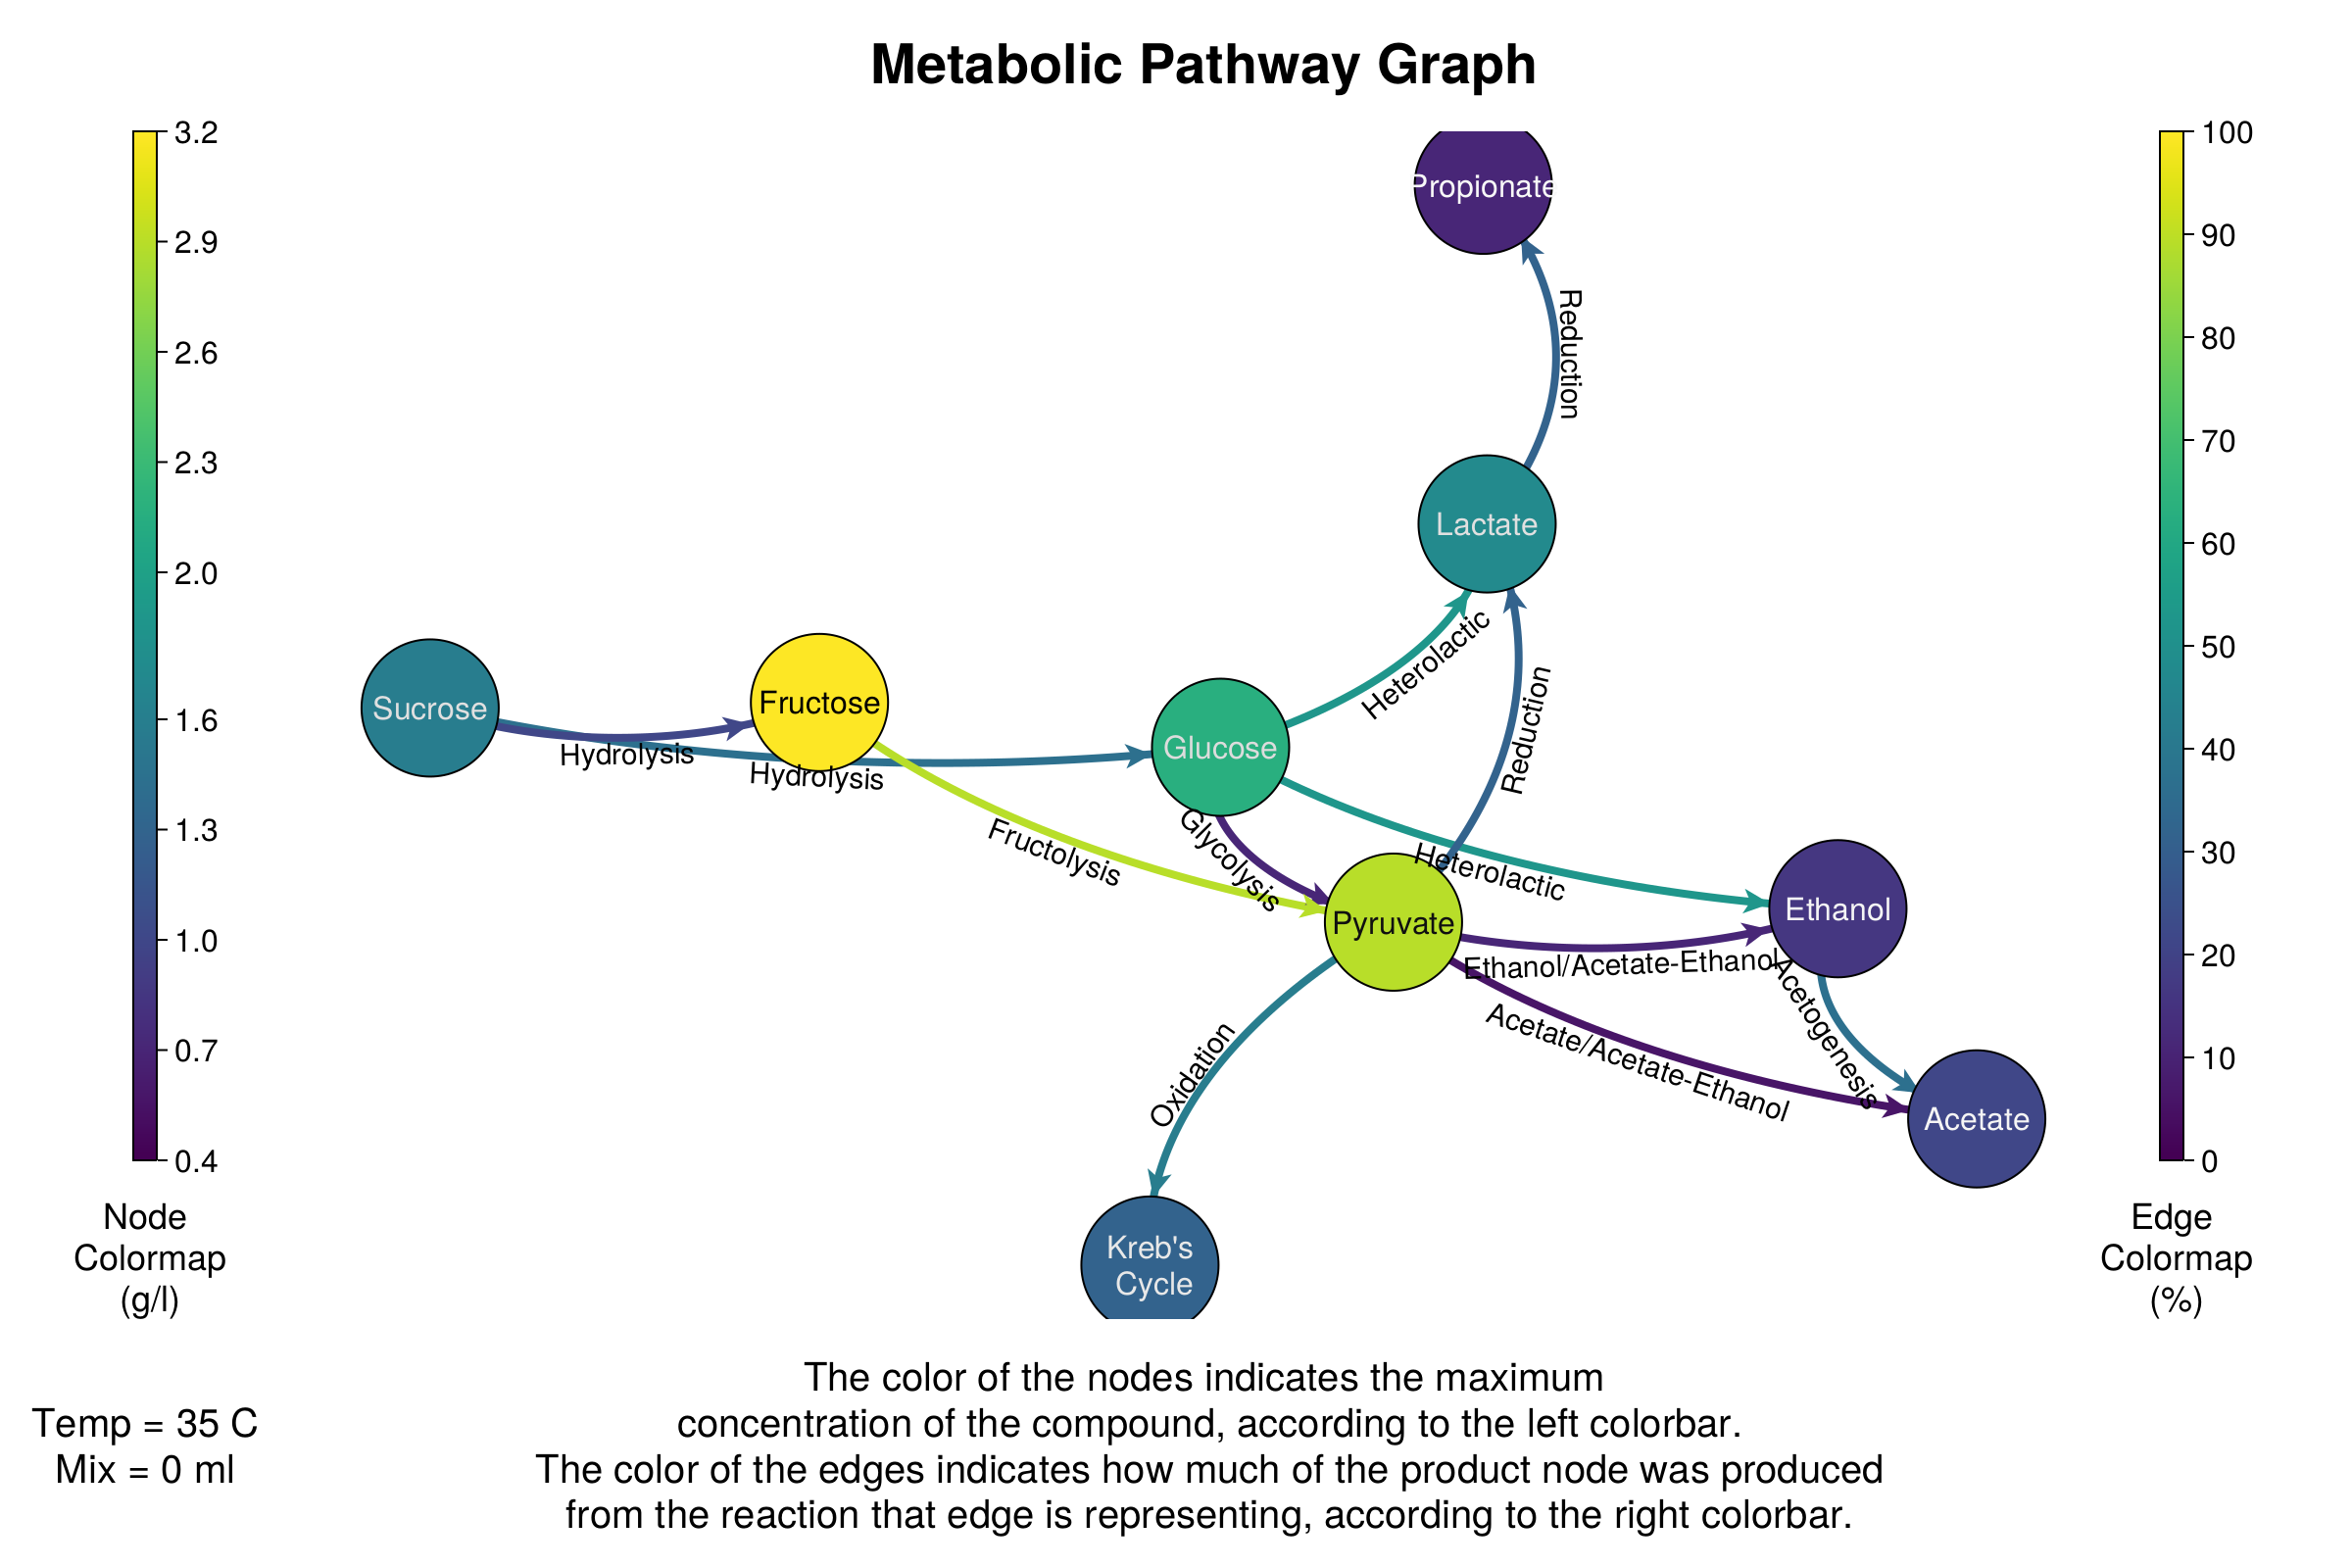
\includegraphics[width=.9\linewidth]{../plots/metabolic_results/35_0.png}
\caption{\label{fig:orga6c82ef}Διάγραμμα Προβλεπόμενου Μεταβολικού Δικτύου}
\end{figure}

Καθώς για τα πειράματα του βασικού σχεδιασμού υπάρχουν άλλα 9 τέτοια διαγράμματα, τα υπόλοιπα δεν παρατίθενται εδώ αλλά στο \href{https://github.com/Vidianos-Giannitsis/masters-thesis/tree/main/plots/metabolic\_results}{Github}.

Από τα διαγράμματα αυτά, μπορούν να προκύψουν πολλά συμπεράσματα για το πως μεταβάλλεται το μεταβολικό μονοπάτι με τις αλλαγές στις λειτουργικές συνθήκες. Αυτά παρουσιάζονται στο επόμενο υποκεφάλαιο με κάποια συγκεντρωτικά διαγράμματα που ενισχύουν τις υποθέσεις αυτές.

\section{Συμπεράσματα Ανάλυσης}
\label{sec:orge3218e9}
Μία σημαντική παρατήρηση που έγινε είναι πως η γλυκόζη η οποία καταναλώνεται στην ετερογαλακτική ζύμωση είναι ένα μεγάλο ποσοστό της συνολικής γλυκόζης και είναι σχεδόν σταθερή με την μεταβολή των συνθηκών (συγκεκριμένα είναι \(0.8 \pm 0.05\) της συνολικής). Αυτό το συμπέρασμα φαίνεται στο Σχήμα \ref{fig:orgf117c61}.

\begin{figure}[htbp]
\centering
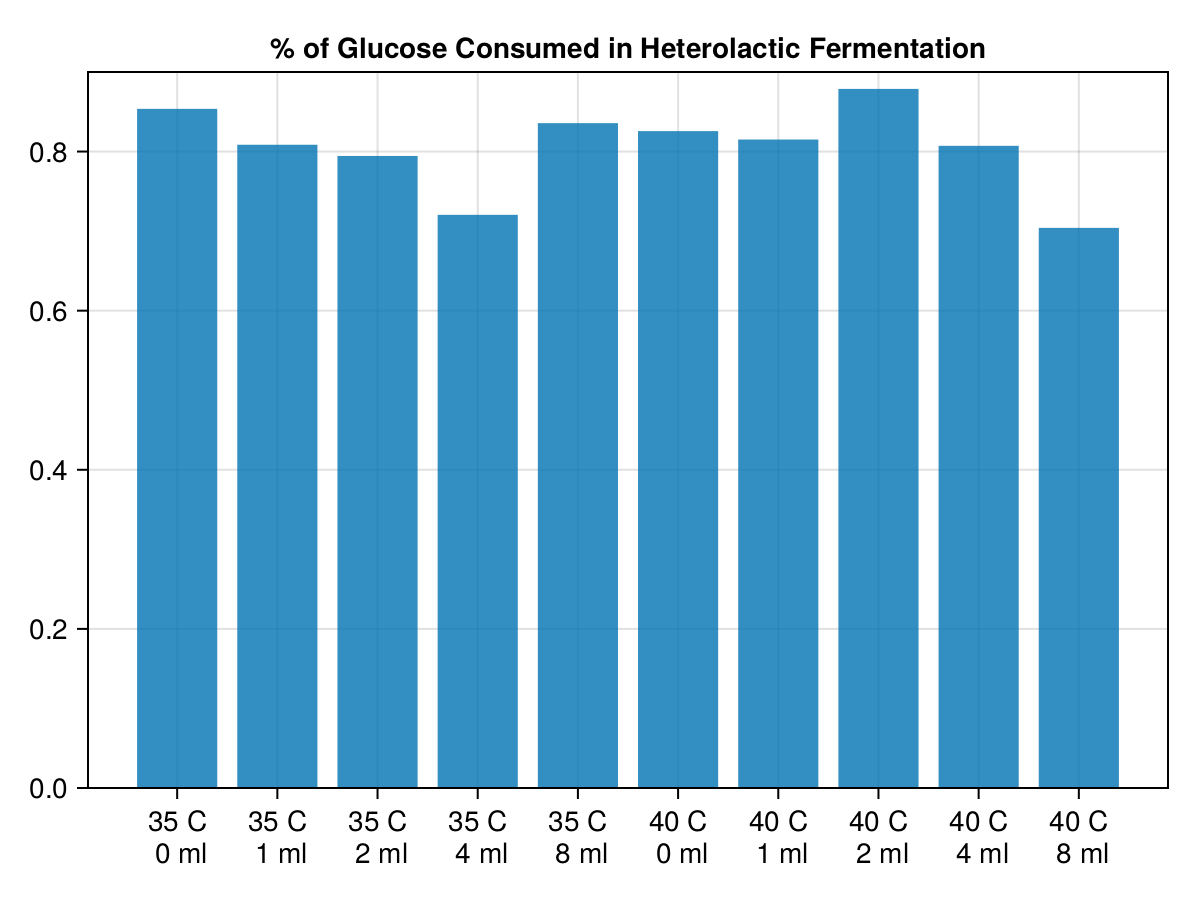
\includegraphics[width=.9\linewidth]{../plots/metabolic_results/heterolactate_flux.png}
\caption{\label{fig:orgf117c61}Ποσοστό γλυκόζης στην ετερογαλακτική ζύμωση}
\end{figure}

Οπότε, θεωρείται πως το μονοπάτι αυτό γίνεται από τους ιθαγενής μικροοργανισμούς (αυτούς που περιέχονται ήδη στο υπόλειμμα τροφών) και επειδή είναι ανεξάρτητο της γλυκόλυσης/φρουκτόλυσης, δεν επηρεάζεται από την προσθήκη άλλων μικροοργανισμών.

Το μεγάλο ποσοστό γλυκόζης προς αυτό το μεταβολικό μονοπάτι εξηγεί κιόλας γιατί σε κάθε αντιδραστήρα βρέθηκε αιθανόλη ακόμη και στους 40 \(^oC\) όπου φάνηκε να αναστέλλεται και είναι ένας από τους λόγους που παράγεται πολύ γαλακτικό. Ακόμη, συμφωνεί με την βιβλιογραφία, η οποία λέει πως οι ιθαγενής μικροοργανισμοί των υπολειμμάτων τροφών είναι συχνά βακτήρια γαλακτικού οξέος, τα οποία μπορούν να καταλύσουν αντιδράσεις παραγωγής και κατανάλωσης του γαλακτικού οξέος.

Οπότε, με βάση αυτή την βιβλιογραφία, αφού όντως οι ιθαγενής μικροοργανισμοί είναι βακτήρια γαλακτικού οξέος, αξίζει να δει κανείς τι γίνεται με την κατανάλωση του γαλακτικού προς προπιονικό οξύ. Στους 35 \(^oC\), το μονοπάτι αυτό έχει αναστολή με την προσθήκη του μιξ, το οποίο μπορεί να σημαίνει πως αυτοί οι μικροοργανισμοί δεν μπορούν να κάνουν την αναγωγή αυτή, αλλά επικρατούν οι αντιδράσεις που καταλύουν καθώς έχουν αυξηθεί, οπότε αυτή χάνεται. Αυτή η υπόθεση ενισχύεται εν μέρει από το γεγονός ότι υπάρχει πολύ μικρή μεταβολή της αντίδρασης αυτής με την προσθήκη του μιξ στους 40 \(^oC\), όμως, η αύξηση όταν προστίθεται το μιξ είναι μεγάλη, οπότε είναι πιθανόν πως υπάρχει κάποιος πιο περίπλοκος μηχανισμός πίσω από την αντίδραση αυτή. Τα αποτελέσματα αυτά παρουσιάζονται στα Σχήματα \ref{fig:org18efba3} και \ref{fig:orgfb36eea}. 

\begin{figure}[htbp]
\centering
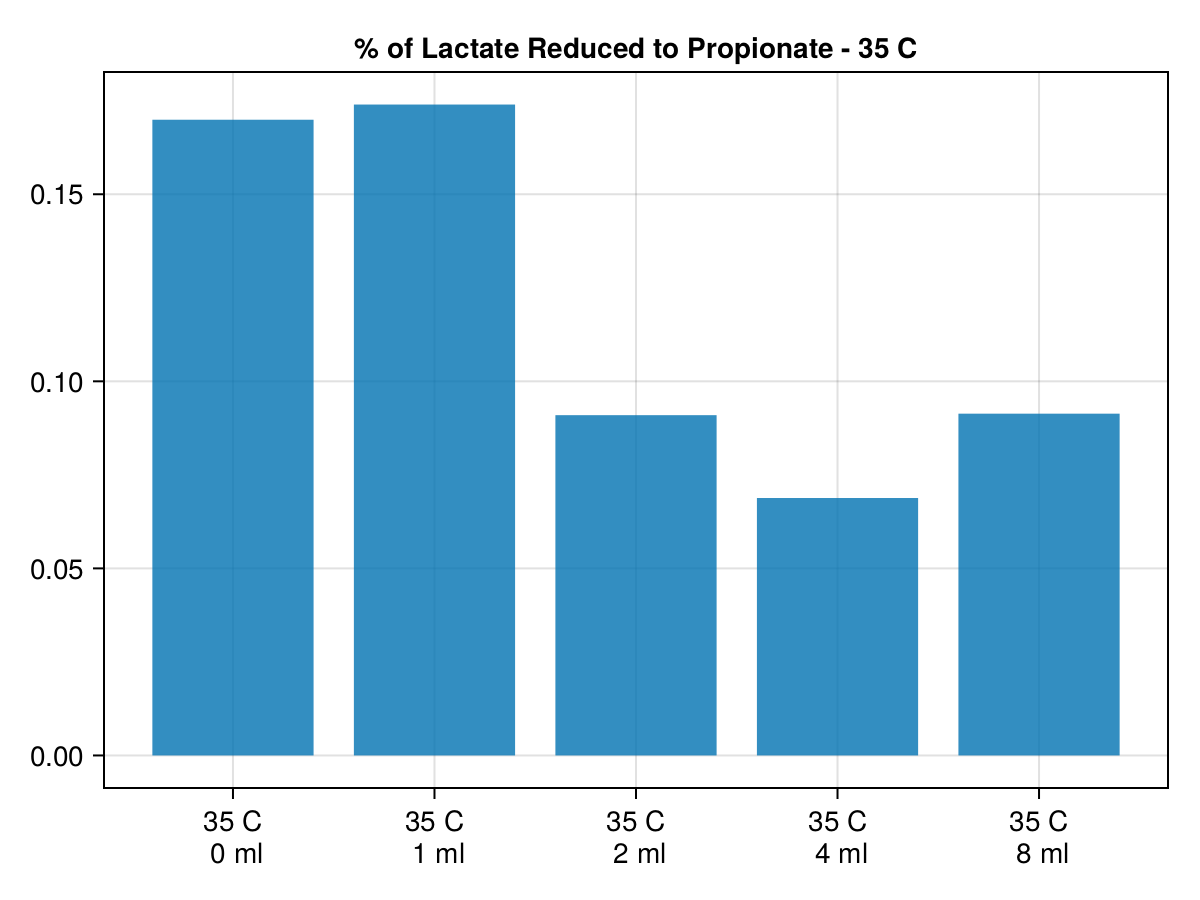
\includegraphics[width=.9\linewidth]{../plots/metabolic_results/propionate_flux_35.png}
\caption{\label{fig:org18efba3}Παραγωγή Προπιονικού - 35 C}
\end{figure}

\begin{figure}[htbp]
\centering
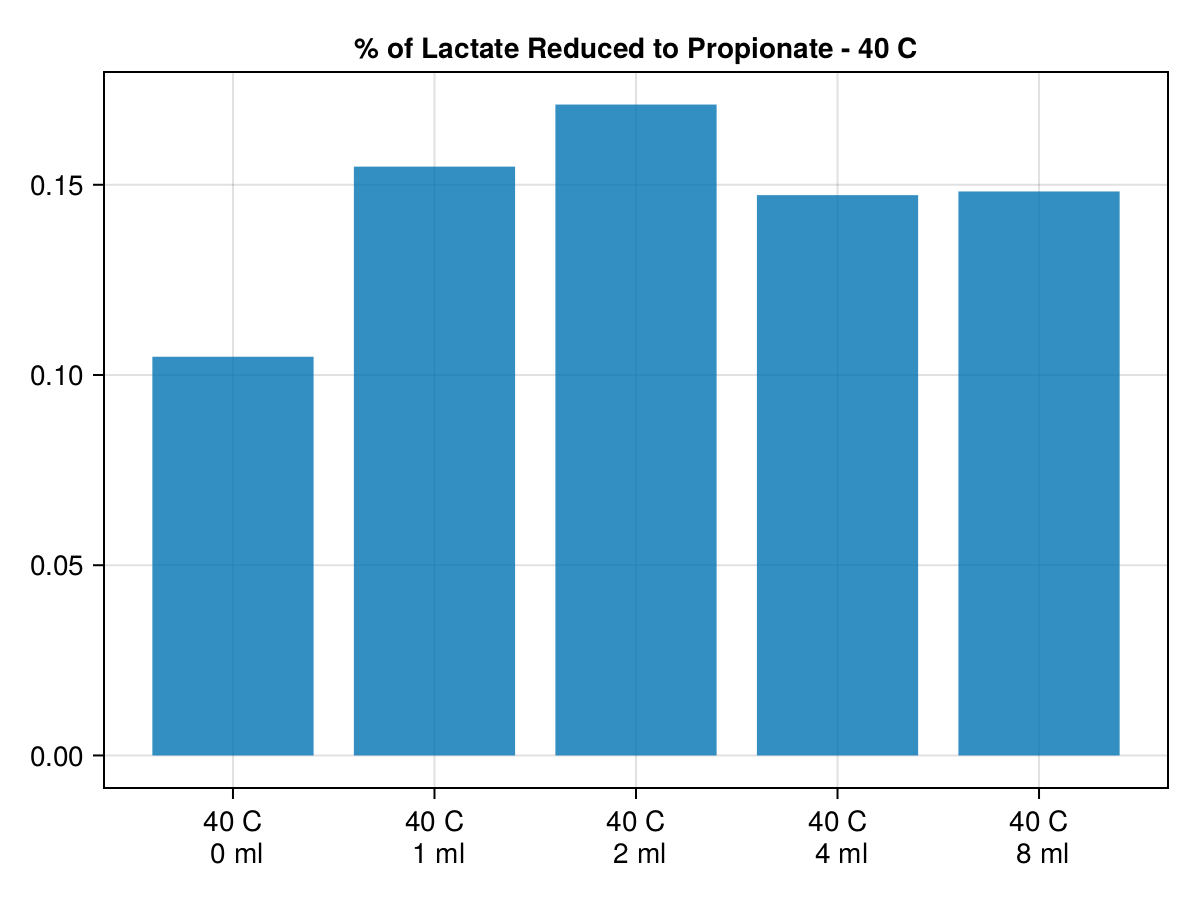
\includegraphics[width=.9\linewidth]{../plots/metabolic_results/propionate_flux_40.png}
\caption{\label{fig:orgfb36eea}Παραγωγή Προπιονικού - 40 C}
\end{figure}

Οι υπόλοιπες αντιδράσεις θεωρείται πως επηρεάζονται είτε άμεσα ή έμμεσα από την προσθήκη του μιξ. Για την υδρόλυση της σακχαρόζης και την γλυκόλυση, αποτελούν δύο γρήγορες αντιδράσεις οι οποίες γίνονται είτε με ή χωρίς παρουσία του μιξ, οπότε, είναι δύσκολο να αποφανθεί αν παίζει ρόλο η προσθήκη του. Θεωρείται όμως πως μπορεί να τις επιταχύνει. Η φρουκτόλυση σίγουρα επηρεάζεται από τους προστιθέμενους μικροοργανισμούς επειδή όπως φαίνεται και στο Σχήμα \ref{fig:org588db03}, οι ιθαγενής μικροοργανισμοί δεν μπορούν να καταναλώσουν αποδοτικά την φρουκτόζη. Οι υπόλοιπες αντιδράσεις σίγουρα θα επηρεάζονται είτε άμεσα ή έμμεσα από την προσθήκη του μιξ, αν αυτό επηρεάζει μία τουλάχιστον, καθώς όλες αποτελούν αντιδράσεις μεταβολισμού του πυροσταφυλικού οξέος. Για καλύτερη σύγκριση τους, παρατίθεται και το Σχήμα \ref{fig:org76e1d65} . 

\begin{figure}[htbp]
\centering
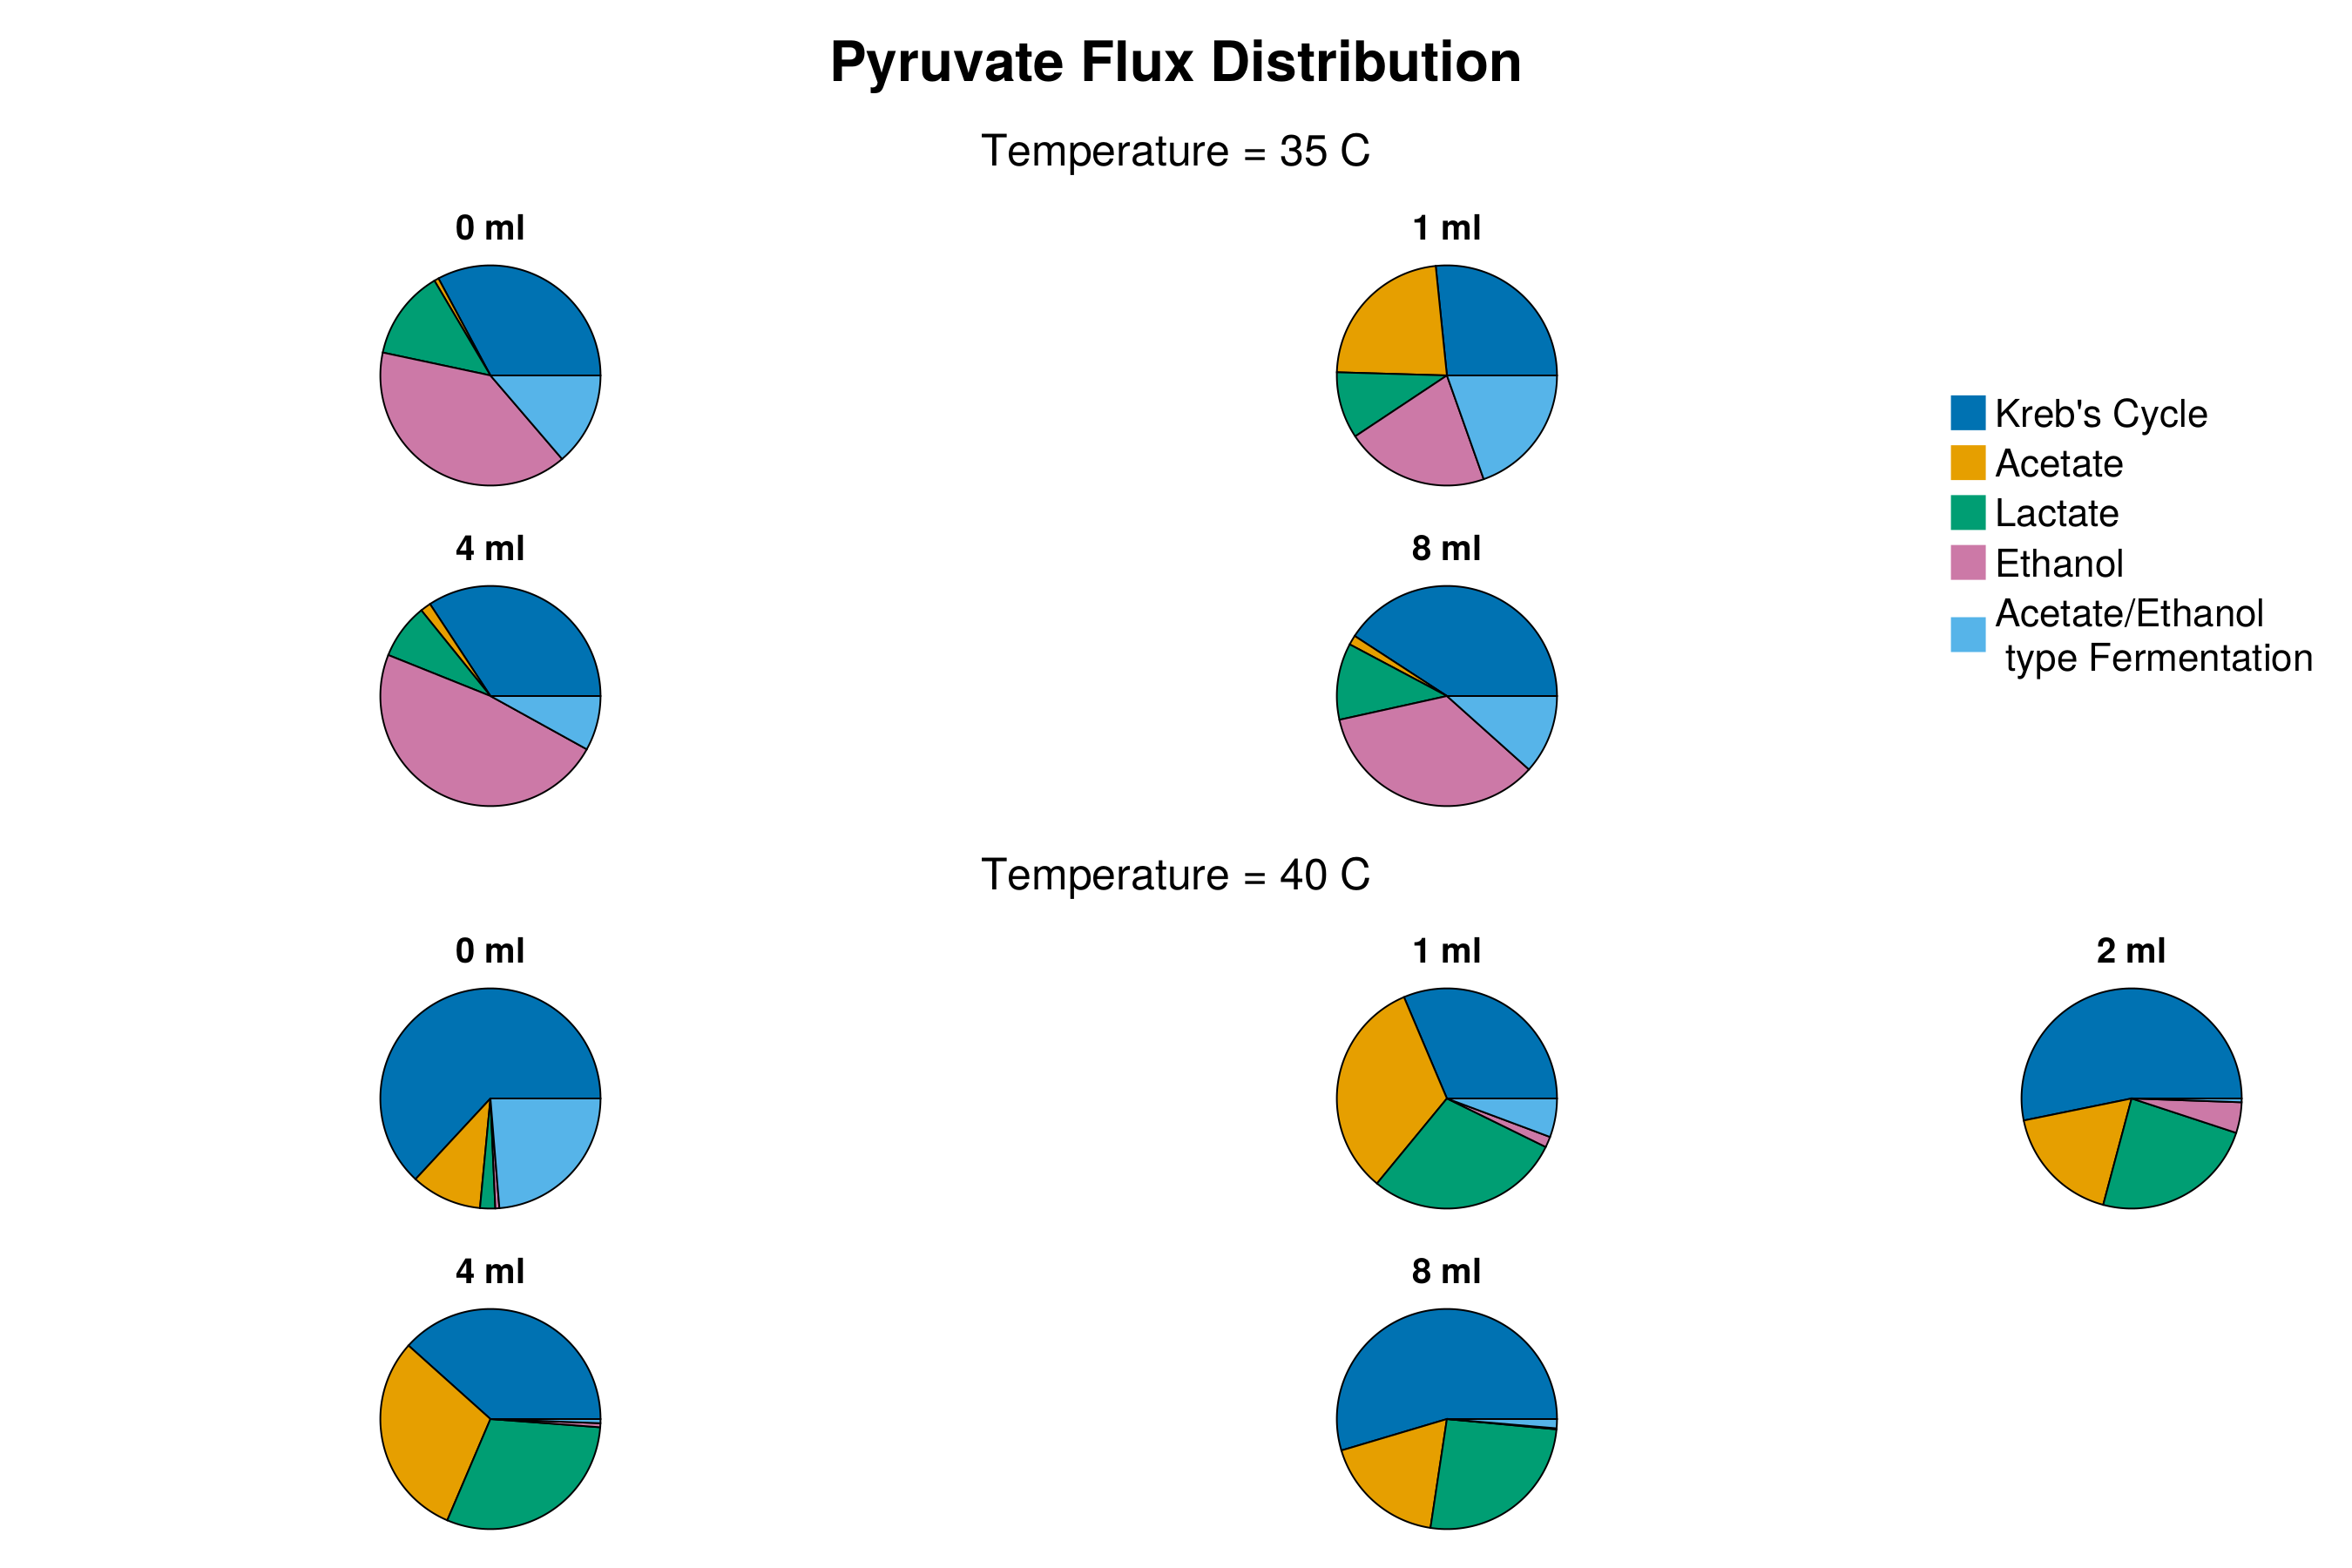
\includegraphics[width=.9\linewidth]{../plots/metabolic_results/pyr_flux_tot.png}
\caption{\label{fig:org76e1d65}Μεταβολισμός του Πυροσταφυλικού Οξέος}
\end{figure}

Από το διάγραμμα αυτό, μπορούν να αναλυθούν σε περισσότερο βάθος κάποιες ενδιαφέρουσες παρατηρήσεις που έχουν γίνει για τα πειράματα αυτά. Μία από τις βασικότερες παρατηρήσεις που είχε γίνει ήταν πως στους 35 \(^oC\) αναστελλόταν η παραγωγή οξικού οξέος ενώ στους 40 \(^oC\) η παραγωγή αιθανόλης. Η αναστολή της παραγωγής αιθανόλης θεωρείται πως είναι απενεργοποίηση των μικροοργανισμών λόγω της υψηλής θερμοκρασίας, ενώ για το οξικό δεν θα μπορούσε να ισχύει αυτό (εφόσον αναστέλλεται στην χαμηλή θερμοκρασία). Οπότε, είχε θεωρηθεί πως η μείωση του οξικού οφείλεται σε κάποια αλληλεπίδραση του με τα άλλα προϊόντα.

Αυτή φαίνεται ξεκάθαρα από το σχήμα αυτό. Στους 35 \(^oC\), το μεγαλύτερο ποσοστό του πυροσταφυλικού μετατρέπεται σε αιθανόλη, με μικρή ποσότητα γαλακτικού καθώς και μικρή ποσότητα μικτής παραγωγής αιθανόλης/οξικού. Αυτό δείχνει πως η προσθήκη του μιξ, ευνοεί την παραγωγή αιθανόλης εώς ένα σημείο και μετά έχει ελάχιστη επίδραση (έτσι και αλλιώς είναι γνωστό πως στους 35 \(^oC\) δεν επέφερε καμία βελτίωση η προσθήκη πάνω από 2 mL μιξ). Η αιθανόλη παράγεται από το Acetyl-CoA μέσω αναγωγής. Επειδή είναι πάρα πολύ ενεργοί οι μικροοργανισμοί αυτοί με την προσθήκη του μιξ, μεταβολίζουν μεγάλο ποσοστό του πυροσταφυλικού και πολύ λίγο Acetyl-CoA μετατρέπεται σε οξικό, και αυτό σε συνδυασμό με αιθανόλη. Η αιθανόλη δεν απαιτεί κάποιο συμπροϊόν κατά τον μεταβολισμό της και το οξικό παράγεται αν τα αναγωγικά μέσα είναι λίγα λόγω της ευκολίας μετατροπής του Acetyl-CoA σε οξικό.

Όταν όμως απενεργοποιούνται οι μικροοργανισμοί αυτοί στους 40 \(^oC\), κύριο προϊόν της διεργασίας γίνεται το άλλο αναγωγικό προϊόν, το γαλακτικό οξύ. Το γαλακτικό οξύ όμως παράγεται από την άμεση αναγωγή του πυροσταφυλικού οξέος, οπότε δεν παράγει αναγωγικά μέσα κατά την παραγωγή του. Ως αποτέλεσμα, υπάρχει ένας οξειδοαναγωγικός περιορισμός στην παραγωγή του γαλακτικού οξέος και παρόλο που η προσθήκη του μιξ το ευνοεί, δεν μπορεί να φτάσει παραπάνω από περίπου \(25-30 \%\) του πυροσταφυλικού για αυτό τον λόγο. Για να αποκατασταθεί η οξειδοαναγωγική ισορροπία από την ευνόηση αυτή του γαλακτικού, είναι αναγκαστικό να παραχθεί το βασικό οξειδωτικό προϊόν του πυροσταφυλικού, το οξικό οξύ. Οπότε, με την προσθήκη του μιξ στην θερμοκρασία αυτή, υπάρχει μία θετική επίδραση στην συγκέντρωση του οξικού οξέος.

Οπότε, φαίνεται πως τα αναγωγικά προϊόντα είναι αυτά που επηρεάζονται άμεσα με θετικό τρόπο από τους μικροοργανισμούς του μιξ, ενώ το οξικό επηρεάζεται έμμεσα επειδή στην μία περίπτωση η αιθανόλη δεν απαιτεί την συμπαραγωγή του ενώ απτην άλλη το γαλακτικό την απαιτεί.

Ένα ακόμη συμπέρασμα, το οποίο είναι αξιοσημείωτο φαίνεται αν ζουμάρουμε στους ιθαγενής μικροοργανισμούς (Σχήμα \ref{fig:org2901647}). Παρόλο που θεωρητικά μπορούν να καταλύσουν και την παραγωγή οξικού και την παραγωγή αιθανόλης, στους 35 \(^oC\) δεν παράγεται καθόλου οξικό από μόνο του (ενώ μπορεί να παραχθεί αν προστεθεί 1 mL μιξ) και αντίστοιχα, η αιθανόλη δεν μπορεί να παραχθεί μόνη της στους 40 \(^oC\), αλλά χωρίς την προσθήκη του μιξ, παράγεται μία ποσότητα μαζί με το οξικό. Οπότε, υπάρχει μία ένδειξη πως οι ιθαγενής μικροοργανισμοί έχουν μία τάση να παράγουν μίγμα οξικού και αιθανόλης (μονοπάτι το οποίο είναι οξειδωαναγωγικά ουδέτερο), ενώ όταν προστίθεται το μιξ, προτιμούνται τα αναγωγικά μονοπάτια, με το οξικό να παράγεται μόνο για την απαραίτητη εξισορρόπηση του οξειδωαναγωγικού δυναμικού.

\begin{figure}[htbp]
\centering
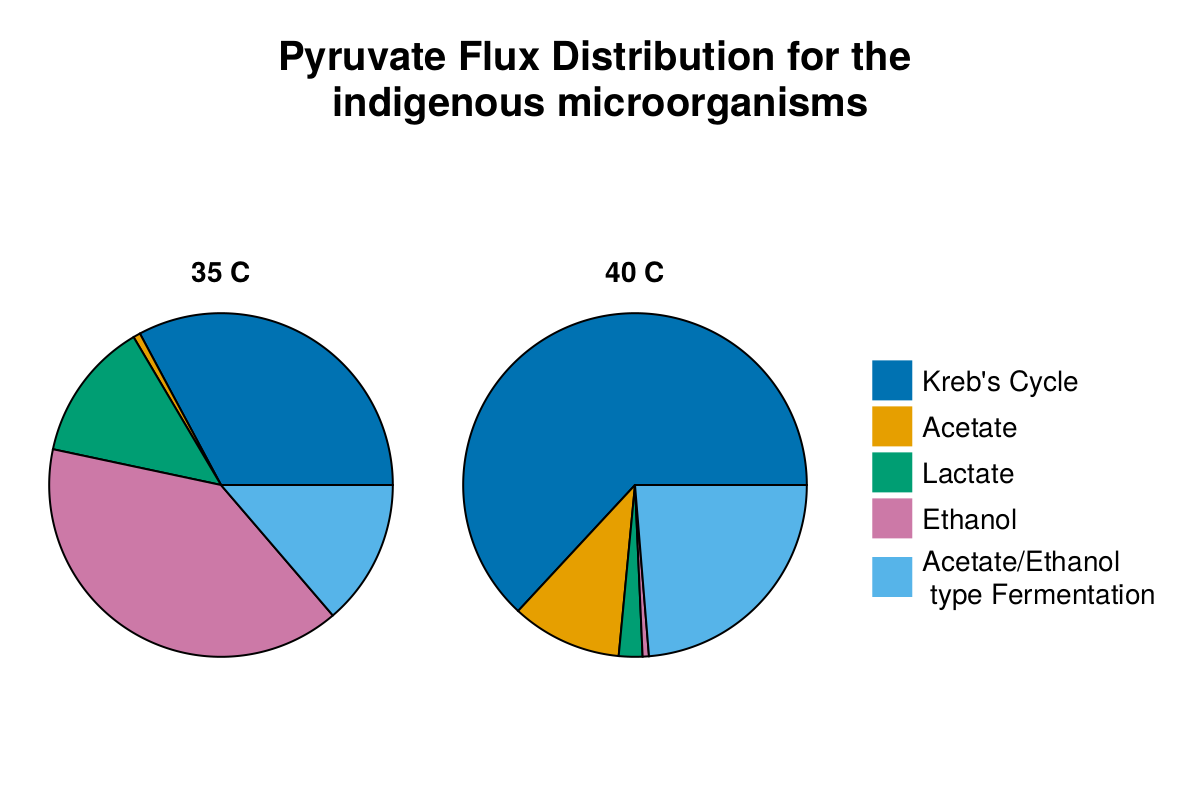
\includegraphics[width=.9\linewidth]{../plots/metabolic_results/pyr_flux_ind.png}
\caption{\label{fig:org2901647}Κατανάλωση πυροσταφυλικού οξέος από τους ιθαγενής μικροοργανισμούς}
\end{figure}
\end{document}
